\documentclass[%
	11pt,
	a4paper,
	utf8,
	%twocolumn
		]{article}	

\usepackage{style_packages/podvoyskiy_article_extended}


\begin{document}
\title{Заметки по машинному обучению и анализу данных}

\author{\itshape Подвойский А.О.}

\date{}
\maketitle

\thispagestyle{fancy}

Здесь приводятся заметки по некоторым вопросам, касающимся машинного обучения, анализа данных, программирования на языках \texttt{Python}, \texttt{R} и прочим сопряженным вопросам так или иначе, затрагивающим работу с данными.


\shorttableofcontents{Краткое содержание}{1}

\tableofcontents

\section{Вопросы}

\subsection{Как строится прогноз в классическом и экстремальной градиентном бустинге?}

\subsection{Как строится поверхность разбиения дерева принятия решения и вычисляется прогноз на дереве}

Для каждого узла дерева принятия решения строится разбиение. ВАЖНО: разбиение строится по какому-то \underline{одному} признаку. Для построения разбиения нужно из всех доступных признаков матрицы признаков, выбрать тот признак и с тем пороговым значением, которые обеспечивают наибольшую эффективность разбиения родительского узла. Например, в задачах классификации в качестве показателя эффективности разбиения можно использовать информационный прирост, вычисленный либо на базе загрязненности Джини, либо на базе энтропии Шеннона. Чем больше информационный прирост, тем <<чище>> дочерние узлы. Или другими словами, чем больше информационный прирост, тем больше экземпляры, попавшие в рассматриваемый узел, похожи друг на друга в смысле значений целевой переменной. В случае задач регрессии, экземпляры обучающего набора данных группируются по показателю разброса вокруг среднего. Чем больше значения вещественной целевой переменной похожи друг на друга (то есть имеют плюс/минус один порядок), тем меньше дисперсия вокруг среднего и тем чище дочерний узел. 

Рекурсивное разбиение данных повторяется до тех пор, пока все точки данных в каждой области разбиения (каждом листе дерева решений) не будут принадлежать одному и тому же значению целевой переменной (классу или количественному значению).

Выход по листу в задаче регрессии вычисляется как среднее арифметическое значений вещественной целевой переменной, ассоциированных с экземплярами обучающего набора данных, попавшими в рассматриваемый лист. В задаче классификации выход по листу строится как среднее арифметическое вероятностей принадлежности экземпляра к определенному классу.

Прогноз для новой точки данных получают следующим образом: сначала выясняют, в какой области разбиения пространства признаков находится данная точка, а затем назначают класс, к которому относится большинство точек в этой области. Область может быть найдена с помощью обхода дерева, начиная с корневого узла, и путем перемещения влево или вправо, в зависимости от того, выполняется ли очередной тест.

В задаче регрессии используется точно такой же подход. Для получения прогноза мы обходим дерево на основе тестов в каждом узле и находим лист, в который попадает новая точка данных. Выходом для этой точки данных будет значение целевой переменной, усредненное по всем \emph{обучающим} точкам в этом листе.

Или другими словами, после прохода по дереву решений и выяснению листа, к которому принадлежит новая точка данных (экземпляр \emph{тестового} набора данных), этой точке данных будет назначен выход листа, вычисленный как среднее арифметическое значений вещественной целевой переменной, ассоциированных с экземплярами \emph{обучающего} набора данных, попавшими в рассматриваемый лист.

ВАЖНО: разбиение строится по значениям \emph{одного} выбранного признака, а <<мера похожести>> экземпляров обучающего набора данных, попавших в узел, и выход по листу строится на основании значений целевой переменной, ассоциированных с экземплярами обучающего набора данных, попавшими в рассматриваемый узел или лист. В результате (для задачи регрессии) поверхность принятия решения представляет собой ступенчатую поверхность, имеющую константное значение в пределах отдельно взятого листа.

\section{Основные термины}

\noindent\emph{Квантиль} -- значение, которое заданная случайная величина не превышает с фиксированной вероятностью. Если вероятность задана в процентах, то квантиль называют процентилем. Пример: фраза <<90-й процентиль массы тела у новорожденных мальчиков составляет 4 кг>>, что означает 90\% мальчиков рождаются с массой тела, меньшей или в частном случае равной 4 кг, а 10\% соответственно -- с массой большей 4 кг. Если распределение непрерывно, то $ \alpha $-квантиль однозначно задается уравнением
\begin{align*}
	F_X(x_\alpha) = \alpha.
\end{align*}

Для непрерывных распределений справедливо следующее широко использующееся при построении доверительных интервалов равенство
\begin{align*}
	\mathbb{P}\big(x_{\frac{1 - \alpha}{2}} \leqslant X \leqslant x_{\frac{1 + \alpha}{2}}\big) = \alpha.
\end{align*}

\noindent\emph{Интерквартильный размах} -- разность между третьим и первым квартилями, то есть $ x_{0,75} - x_{0,25} $. Интерквартильный размах является характеристикой разброса и является робастным аналогом дисперсии. Вместе, медиана и интерквартильный размах могут быть использованы вместо математического ожидания и дисперсии в случае распределений с большими выбросами.

\noindent\emph{Web-сокет} -- это технология, позволяющая создавать интерактивное соединение для обмена сообщениями в режиме реального времени. Web-сокет в отличие от HTTP не нуждается в повторяющихся запросах к серверу. Сокет работает таким образом, что достаточно лишь один раз выполнить запрос, а потом ждать отклика. То есть можно спокойно слушать сервер, который отправит сообщения по мере готовности. Сокеты применяют приложениях, обрабатывающих информацию в <<реальном времени>> (IoT-приложения, чаты и пр.)

\noindent\emph{Функции высшего порядка} -- это функции, которые могут принимать другие функции в качестве значений своих аргументов или возвращать другие функции в качестве своего результата.

\noindent\emph{Функции первого класса} -- это функции, которые \emph{трактуются как объекты}. Такие функции можно передавать другим функциям в качестве значений аргументов, возвращать из других функций или сохранять в переменных.

\section{Оценка потребления ресурсов Python-приложением}

Оценить потребление ресурсов Python-приложением можно с помощью модуля \texttt{memory\_profiler}\footnote{Ставится как обычно с помощью \texttt{pip}: \texttt{pip install memory\_profiler}}
\begin{lstlisting}[
style = ironpython,
numbers = none
]
from memory_profiler import memory_usage

print(memory_usage())
\end{lstlisting}

\section{Теория алгоритмов и структуры данных}

В \emph{теории сложности вычислений} широкое распространение получило обозначение <<\emph{О}-большое>>. Типичный результат выглядит следующим образом: <<данный алгоритм работает за время $ O(n^2 \log n) $>>, и его следует понимать как <<существует такая константа $ C > 0 $, что \emph{время работы} алгоритма в \emph{наихудшем} случае не превышает $ C\,n^2 \log n $, начиная с некоторого $ n $>>.

Практическая ценность асимптотических результатов такого рода зависит от того, насколько мала неявно подразумеваемая константа $ c $. Как мы уже отмечали выше, для подавляющего большинства известных алгоритмов она находится в разумных пределах, поэтому, как правило, имеет место следующий тезис: алгоритмы, более эффективные с точки зрения их асимптотического поведения, оказываются также более эффективными и при тех сравнительно небольших размерах входных данных, для которых они реально используются на практике. Другими словами, \emph{асимптотические оценки эффективности} достаточно полно отражают реальное положение вещей.

Теория сложности вычислений по определению считает, что алгоритм, работающий за время $ O(n^2 \log n) $ лучше алгоритма с временем работы $ O(n^3) $, и в подавляющем большинстве случаев это отражает реально существующую на практике ситуацию.

Обозначение $ O $-большое распределяет алгоритмы по группам согласно их асимптотическим временам работы \emph{в худшем случае}, таким как линейно-временные ($ O(n) $) или логарифмически-временные ($ O(n \log n) $) алгоритмы и операции \cite[246]{roughgarden-graph:2019}.

Смысл \emph{структуры данных} заключается в организации данных таким образом, чтобы к ним можно было получить доступ быстро и с пользой. Например, \emph{очередь} последовательно организует данные так, что удаление объекта в ее начале или добавление объекта в ее конце занимает \emph{постоянное время}. \emph{Стек} в качестве структуры данных позволяет удалять объект или добавлять объект в его начало за \emph{постоянное время}.

\subsection{Хеш-таблицы}

Хеш-таблица представляет собой эффективную структуру данных для реализации словарей. Хотя поиск элемента в хеш-таблице может в \emph{наихудшем} случае потребовать столько же времени, сколько на поиск в связанном списке, на практике хеширование исключительно эффективно. При вполне обоснованных допущениях \emph{среднее} время поиска элемента в хеш-таблице составляет $ O(1) $ \cite[285]{cormen-algo:2013}.

Хеш-таблицы, подобно кучам и деревьям поиска, поддерживают эволюционирующее множество объектов, ассоциированных с ключами. В отличие от кучи и деревьев поиска, они не поддерживают никакой информации об упорядочивании вообще. Смысл существования хеш-таблицы состоит в том, чтобы \emph{облегчить сверхбыстрый поиск} (по ключу), который также в этом контексте называется просмотром (lookup). Хеш-таблица может сказать, что в ней есть, а чего нет, и может сделать это очень и очень быстро (намного быстрее, чем куча или дерево поиска).

Концептуально хеш-таблицу можно рассматривать как \emph{массив} \cite{roughgarden-graph:2019}. Единственно, чем хороши массивы, -- это немедленным случайным к ним доступом. В массиве, чтобы, например, узнать что находится в позиции или изменить значение в этой позиции нужно просто обратиться к этой позиции за постоянное время. \emph{Массивы} прекрасно подходят для \emph{чтения элементов} в произвольных позициях, потому что обращение к любому элементу в массиве происходит мгновенно. \emph{Связанные списки} отлично подходят в тех ситуациях, когда данные должны читаться \emph{последовательно}: сначала читается один элемент, по адресу переходим к следующему элементу и т.д. Хеш-таблицы сочетают в себе лучшие возможности массивов и связанных списков.

\textbf{Когда использовать хеш-таблицу}: если приложению требуется \emph{быстрый поиск} с динамически изменяющимся множеством объектов, то хеш-таблица обычно является предпочтительным вариантом.

Быстродействие хеш-таблиц
\begin{itemize}
	\item \emph{поиск}:
	\begin{itemize}
		\item в \underline{среднем} операция выполняется за постоянное время $ O(1) $,
		
		\item в \underline{худшем} случае -- за время $ O(n) $,
	\end{itemize}
	
	\item \emph{вставка}:
	\begin{itemize}
		\item в \underline{среднем} операция выполняется за постоянное время $ O(1) $,
		
		\item в \underline{худшем} случае -- за время $ O(n) $,
	\end{itemize}

    \item \emph{удаление}
    \begin{itemize}
    	\item в \underline{среднем} операция выполняется за постоянное время $ O(1) $,
    	
    	\item в \underline{худшем} случае -- за время $ O(n) $,
    \end{itemize}
\end{itemize}

Для достижения постоянно-временного \emph{поиска} в хеш-таблице со сцеплением списки корзин должны оставаться \underline{короткими}, в идеале -- с длиной не более малой константы \cite[212]{roughgarden-graph:2019}.

ВАЖНО: любые операции в хеш-таблицах \emph{в среднем} выполняются за \underline{постоянное}\footnote{Постоянное время не означает, что операции выполняются мгновенно; просто время остается постоянным независимо от размера хеш-таблицы} время $ O(1) $, а в худшем -- за \emph{линейное} время $ O(n) $ (это очень медленно).

Для разрешения коллизий в хеш-таблицах, как правило, используется:
\begin{itemize}
	\item либо стратегия с использованием \emph{связанных списков} (список может быть как однонаправленным, так и двунаправленным),
	
	\item либо стратегия с использованием \emph{метода открытой адресации} (линейное исследование, квадратичное исследование, двойное хеширование).
\end{itemize}

ВАЖНО: для предотвращения коллизий необходимы:
\begin{itemize}
	\item низкий коэффициент загрузки $ \alpha = n/b $, где $ n $ -- число элементов коллекции, а $ b $ -- число ячеек хеш-таблицы,
	
	\item хорошая хеш-функция.
\end{itemize}

В хеш-таблице с \emph{открытой адресацией} время выполнения операции чтения или вставки масштабируется вместе с числом проб, необходимых для отыскания пустой ячейки (либо искомого объекта). Когда коэффициент загрузки хеш-таблицы равен $ \alpha $, то это означает, что $ \alpha $-доля ячеек хеш-таблицы заполнена, а оставшаяся часть $ (1 - \alpha) $ является пустой.

В поиске на основе хеша $ n $ элементов коллекции $ C $ сначала загружаются в хеш-таблицу $ H $ с $ b $ ячейками (еще их называют <<корзинами>>), структурированными в виде массива. Этот шаг предварительной обработки имеет производительность $ O(n) $, но улучшает производительность будущих поисков с использованием концепции хеш-функции. 

\emph{Хеш-функция} представляет собой детерминированную функцию, которая отображает каждый элемент $ C_i $ коллекции на целочисленное значение $ h_i $ (индекс ячейки в хеш-таблице). На минуту предположим, что $ 0 \leqslant h_i < b $. При загрузке элементов в хеш-таблицу элемент $ C_i $ вставляется в ячейку $ H[h_i] $. После того как все элементы будут вставлены, поиск элемента $ t $ становится поиском $ t $ в $ H[hash(t)] $.

Хеш-функция гарантирует только, что если два элемента, $ C_i $ и $ C_j $, равны, то $ hash(C_i) = hash(C_j) $. Может случиться так, что несколько элементов в коллекции $ C $ имеют одинаковые значения хеша; такая ситуация называется \emph{коллизией}, и хеш-таблице необходима стратегия для урегулирования подобных ситуаций.

ВАЖНО: размер хеш-таблицы следует увеличить, если \emph{коэффициент загрузки} $ \alpha $ начинает превышать 0.70 (это хорошее эмпирическое правило); тогда, при наличии правильно выбранной хеш-функции и непаталогических данных, все наиболее распространенные стратегии разрешения коллизий, как правило, приводят к постоянно-временным хеш-табличным операциям \cite[225]{roughgarden-graph:2019}.

Наиболее распространенным решением является хранение в каждой ячейке \emph{связанного списка} (несмотря на то, что \emph{многие} из этих связанных списков будут содержать \emph{только один элемент}); при этом в хеш-таблице могут храниться все элементы, вызывающие коллизии.

Поиск в связанных списках должен выполняться линейно, но он будет \emph{быстрым}, потому что каждый из них может хранить максимум несколько элементов. При поиске на основе хеша количество сравнений строк \emph{связано с длиной связанных списков}, а не с размером коллекции.

Целочисленный индекс ячейки в хеш-таблице для элемента $ s $ вычисляется как
\begin{align*}
	hash(s) = \abs{hashFun(s)} \mod b,
\end{align*}
где $ hashFun(s) $ -- хеш-функция от элемента, $ b $ -- число ячеек в хеш-таблице.

Первичная память хеш-таблицы $ H $ должна быть достаточно большой, а \emph{связанные списки элементов}, хранящиеся в ячейках, должны быть как можно \emph{меньше}.

В качестве размера хеш-таблицы $ H $ обычно выбирается простое число, чтобы гарантировать, что использование оператора вычисления остатка от деления эффективно распределяет вычисляемые номера ячеек. На практике хорошим выбором является $ 2^k - 1 $, несмотря на то что это значение не всегда простое.

ВАЖНО: вставка элемента в связанный список выполняется за постоянное время, а удаление элемента пропорционально длине списка. Если хеш-функция равномерно распределяет элементы, отдельные списки оказываются относительно короткими.

После того как хеш-функция возвращает \emph{индекс ячейки} в хеш-таблице, мы смотрим, пуста ли соответствующая ячейка таблицы. Если она пуста, возвращаем значение \texttt{False}, указывающее, что искомого элемента нет в коллекции. В противном случае просматриваем связанный список для этой ячейки, чтобы определить наличие или отсутствие в нем искомого элемента.

\emph{Среднее} время, необходимое для \emph{поиска} элемента, является константой, или $ O(1) $. Поиск состоит из одного просмотра $ H $ с последующим линейным поиском в коротком списке коллизий.

Определим для хеш-таблицы \emph{коэффициент загрузки} $ \alpha $ как среднее количество элементов в связанном списке для некоторой ячейки $ H[h] $. Точнее, $ \alpha = n/b $, где $ n $ -- количество элементов отображаемой коллекции, а $ b $ -- количество ячеек в хеш-таблице.

ВАЖНО: По мере увеличения числа ячеек $ b $ в хеш-таблице \emph{максимальная} длина связанных списков \emph{уменьшается}, а количество ячеек, содержащих единственный элемент увеличивается.

ВАЖНО: По мере уменьшения коэффициента загрузки $ \alpha = n/b $ средняя длина каждого списка элементов также уменьшается, что приводит к улучшению производительности. То есть при фиксированном количестве элементов коллекции чем больше ячеек в хеш-таблице, тем лучше.

Так как хеш-таблица обычно может расти до размера, достаточно большого, чтобы все \emph{связанные списки элементов были небольшими}, производительность поиска считается равной $ O(1) $.

Один популярный вариант поиска на основе хеша модифицирует обработку коллизий путем наложения ограничения, заключающегося в том, что \emph{каждая ячейка} содержит \emph{один элемент}.

Вместо создания \emph{связанного списка} для хранения всех элементов, которые хешируются в одну и ту же ячейку в хеш-таблице, используется \emph{метод открытой адресации}, который хранит элементы, вызвавшие коллизию, \emph{в некотрых других пустых ячейках хеш-таблицы} $ H $ \cite[140]{heineman:2017}.

При использовании открытой адресации хеш-таблица снижает накладные расходы на хранение элементов путем устранения всех связанных списков.

Чтобы \emph{вставить} элемент с использованием открытой адресации, вычисляется индекс ячейки в хеш-таблице $ h_k = hash(e) $, которая должна содержать элемент $ e $. Если ячейка $ H[h_k] $ пуста, ей присваивается значение элемента $ H[h_k] = e $ так же, как и в стандартном алгоритме. В противном случае выполняется \emph{исследование} (probe) ячеек $ H $ с использованием той или иной стратегии исследования и элемент $ e $ помещается в первую обнаруженную пустую ячейку.

Стратегии исследований:
\begin{itemize}
	\item Линейное исследование; выполняется неоднократный поиск в ячейках $ h_k = (h_k + c\cdot i) \mod b $, где $ c $ -- целочисленное смещение, а $ i $ -- количество последовательных исследований $ H $ (часто $ c = 1 $); при использовании этой стратегии в $ H $ могут появится кластеры элементов,
	
	\item Квадратичное исследование; выполняется неоднократный поиск в ячейках $ h_k = (h_k + c_1 \cdot i + c_2 \cdot i^2) \mod b $, где $ c_1 $ и $ c_2 $ -- константы; этот подход обычно позволяет избежать кластеризации; полезными для практического применения являются значения $ c_1 = c_2 = 1/2 $,
	
	\item Двойное хеширование; сходно с линейным исследованием, но в отличие от него $ c $ не является константой, а определяется второй хеш-функцией.
\end{itemize}

ВАЖНО: Во всех случаях, если пустая ячейка после $ b $ проб не обнаружена, вставка считается неудачной.

В хеш-таблице с использованием открытой адресации \emph{проблемой} является \emph{удаление} элементов. Для поддержки удаления при использовании открытой адресации необходимо пометить ячейку как удаленную.

Открытая адресация уменьшает общее количество используемой памяти, но требует существенно большего количества проб в наихудшем случае. Второе следствие заключается в том, что линейное исследование приводит к большему количеству проб из-за кластеризации.

Вычисленный коэффициент загрузки для хеш-таблиц описывает ожидаемую производительность \emph{поиска} и \emph{вставки}. Если коэффициент загрузки слишком высок, количество проб при поиске элемента становится чрезмерным, будь то в связанном списке ячейки или в цепочке ячеек при использовании открытой адресации. Хеш-таблица может увеличить количество ячеек и перестроится с помощью процесса, известного как <<перехеширование>> -- нечастой операции, которая уменьшает коэффициент загрузки, хотя и является дорогостоящей операцией, -- со временем работы $ O(n) $.

Типичный способ изменения размера -- удвоить количество имеющихся ячеек и добавить еще одну (так как хеш-таблицы обычно содержат нечетное количество ячеек). Когда становится доступным большее количество ячеек, все существующие элементы в хеш-таблице перехешируются и вносятся в новую структуру. Эта дорогостоящая операция снижает общую стоимость будущих поисков, но должна выполняться как можно реже; в противном случае не удастся получить амортизационную производительность хеш-таблиц, равную $ O(1) $. 

Выбор стратегии разрешения коллизий зависит от многих обстоятельств. Например, сценарий разрешения коллизий на базе связанных списков занимает больше места, чем открытая адресация (для хранения указателей в связанных списках), поэтому открытая адресация может быть предпочтительнее, когда пространство является первоочередной проблемой. Реализация удалений выполняется сложнее с открытой адресацией, чем со сцеплением, поэтому сцепление может быть предпочтительнее в приложениях с большим числом удалений.

ВАЖНО: поскольку хеш-таблицы с открытой адресацией хранят не более одного объекта в расчете на позицию в массиве, у них никогда не может быть коэффициента загрузки больше 1. Как только коэффициент загрузки стал равен 1, вставить больше объектов уже не получится. А вот в хеш-таблицу со сцеплением может быть вставлено произвольное число объектов, хотя ее результативность снижается по мере вставки большего числа объектов. Например, если загрузка равна 100, то средняя длина списка корзины тоже равна 100 \cite{ramalho:python-2016}.


\subsection{Фильтры Блума}

Фильтр Блума предоставляет альтернативную структуру \emph{битового массива} $ B $, которая обеспечивает константную производительность при добавлении элементов из коллекции $ C $ в битовый массив $ B $ или проверку того, что элемент \emph{не был добавлен} в битовый массив $ B $. 

Как ни удивительно, это поведение не зависит от количества элементов, уже добавленных в $ B $. Однако имеется и ловушка: при проверке, находится ли некоторый элемент в $ B $, фильтр Блума может возвратить ложно-положительный результат, даже если на самом деле элемент в $ C $ отсутствует. Фильтр Блума позволяет \emph{точно} определить, что элемент \underline{не был добавлен} в $ B $, поэтому никогда не возвращает ложно-отрицательный результат.

На \pic{fig:filter_blum} в битовый массив $ B $ вставлены два значения, $ u $ и $ v $. Таблица в верхней части рисунка показывает позиции битов, вычисленные хеш-функциями ($ k = 3 $). Как можно видеть, фильтр Блума в состоянии быстро определить, что третье значение $ w $ не было вставлено в битовый массив $ B $, поскольку одно из его $ k $ вычисляемых значений битов равно нулю (в данном случае это бит с позицией 6). Однако для значения $ x $ фильтр возвращает ложно-положительный результат, поскольку, несмотря на то что это значение не было вставлено в $ B $, все $ k $ вычисляемых битов равны единицы.

\begin{figure}[h]
	\centering
	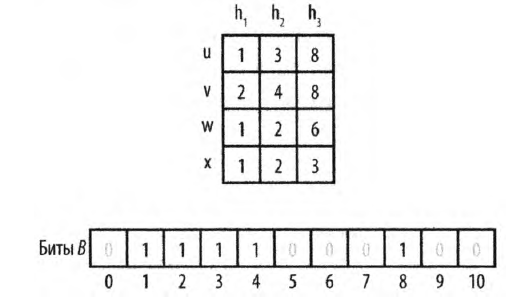
\includegraphics[scale=0.85]{figures/filter_blum.png}
	\caption{ Пример работы фильтра Блума }\label{fig:filter_blum}
\end{figure}

Фильтр Блума обрабатывает значения во многом так же, как и поиск на основе хеша. Алгоритм начинает работу с массива из $ m $ битов, каждый из которых изначально равен нулю. Имеется $ k $ хеш-функций, вычисляющих при вставке значений (потенциально различные) позиции битов в этом массиве.

Фильтр Блума возвращает значение false, если может доказать, что целевой элемент $ t $ еще не был вставлен в битовый массив и, соответственно, отсутствует в коллекции $ C $. Алгоритм может вернуть значение true, которое может быть ложно-положительным результатом, если искомый элемент $ t $ был вставлен в массив. То есть если хотя бы один из битов имеет значение 0, значит, искомое значение не было добавлено в массив, однако, если все $ k $ битов имеют значение 1, можно только утверждать, что искомое значение \emph{могло} быть добавлено в массив.

ВАЖНО: Фильтр Блума демонстрирует эффективное использование памяти, но он полезен только тогда, когда допустимы ложно-положительные результаты. 

Общее количество памяти, необходимое для работы фильтра Блума, фиксировано и составляет $ m $ битов, и оно не увеличивается независимо от количество хранящихся значений. Кроме того, алгоритм требует только фиксированного количества испытаний $ k $, поэтому каждая вставка и поиск могут быть выполнены за время $ O(k) $, которое рассматривается как константное \cite[149]{heineman:2017}.

Основная сложность фильтра заключается в разработке эффективных хеш-функций, которые обеспечивают действительно равномерное распределение вычисляемых битов для вставляемых значений. Хотя размер битового массива является константой, для снижения количества ложно-положительных срабатываний он может быть достаточно большим. И, наконец, нет никакой возможности удаления элемента из фильтра, поскольку потенциально это может фатально нарушить обработку других значений.

Фильтр Блума имеет предсказуемую \emph{вероятность ложно-положительного срабатывания} в предположении, что $ k $ хеш-функций дают равномерно распределенные случайные величины. Достаточно точной оценкой $ p_k $ является следующая \cite[\strbook{149}]{heineman:2017}
\begin{align*}
	p_k = \dfrac{1}{2} \Bigg[ 1 - \bigg( 1 - \dfrac{1}{m} \bigg)^{kn} \Bigg]^k,
\end{align*}
где $ k $ -- число хеш-функций; $ m $ -- длина битового массива (размер фильтра Блума в битах); $ n $ -- количество добавленных в фильтр значений.

Если требуется, чтобы ложно-положительные срабатывания не превышали некоторого небольшого значения, следует выбрать $ k $ и $ m $ после оценки числа $ n $ вставляемых элементов. В литературе предлагается обеспечить значение $ 1 - (1 - 1/m)^{kn} $, близкое к 1/2.
Например, чтобы гарантировать, что ложно-положительные срабатывания для списка из 211 422 будут для менее 10\%, следует установить значение $ m $ равным по крайней мере 1 120 000 битам.

Фильтр Блума поддерживает операции Вставить и Просмотреть (Поиск) в \emph{постоянной времени} и он предпочтительнее хеш-таблиц в приложениях, в которых пространство ценится не вес золота, а периодические ложные утверждения не являются проблемой.



\subsection{Кучи}

\emph{Куча} -- структура данных, которая отслеживает эволюционирующее множество объектов с \emph{ключами} и может быстро идентифицировать объект с наименьшим ключом.

Самые главные вещи, которые следует помнить о любой структуре данных, -- это операции, которые она поддерживает, и время, необходимое для каждой из них.

Две самые важные операции, поддерживаемые кучами, это операции
\begin{itemize}
	\item \textsf{Вставить},
	
	\item \textsf{Извлечь минимум}\footnote{Структуры данных, поддерживающие эти операции, также называют \emph{очередями с приоритетом}}
\end{itemize}

ВАЖНО: Алгоритм HeapSort использует кучу для сортировки массива длины $ n $ за время $ O(n \log n) $.

ВАЖНО: Кучи могут быть визуализированы как полные бинарные деревья, но реализованы в виде массивов.

Было бы легко поддерживать только операцию \textsf{Вставки}, повторно присоединяя новые объекты в конец массива или связанного списка (за постоянное время). Проблема в том, что операция \textsf{Извлечь минимум} требует линейно-временного исчерпывающего поиска по всем объектам. Ясно также как поддерживать только операцию \textsf{Извлечь минимум} -- отсортировать исходное множество $ n $ объектов по ключу заранее раз и навсегда (с использованием времени $ O(n \log n) $ на предобработку), а затем последовательно вызывать операцию \textsf{Извлечь минимум} выхватывания объектов по одному с начала отсортированного списка (каждая за постоянное время). Загвоздка здесь в том, что любая простая реализация операции \textsf{Вставить} требует линейного времени. Хитрость кроется в разработке структуры данных, которая позволяет \emph{обеим} операциям выполняться очень быстро. Именно в этом заключается смысл существования кучи.

\noindent\textbf{Теорема} (Время выполнения основных операций кучи). В куче с $ n $ объектами операции \textsf{Вставить} и \textsf{Извлечь минимум} выполняются за время $ O(\log n) $.

ВАЖНО: {\color{blue}Ни один из вариантов кучи не поддерживает операции \textsf{Извлечь минимум} и \textsf{Извлечь максимум} одновременно за $ O(\log n) $ -- нужно выбрать, какой вариант требуется\footnote{Если нужно иметь обе, то можно использовать одну кучу каждого типа, либо обновить представление данных до сбалансированного дерева поиска}}.

\noindent\textbf{Теорема} (Время выполнения дополнительных кучевых операций). В куче с $ n $ объектами операции \textsf{Найти минимум}, \textsf{Объединить} в кучу и \textsf{Удалить} выполняются за время $ O(1) $, $ O(n) $ и $ O(\log n) $ соответственно.

Обобщим и приведем итоговый перечень показателей для куч на \pic{fig:heap}. В случае операции \textsf{Извлечь минимум} нам нужно найти объект с наименьшим ключом, удалить его из кучи, а затем вернуть -- то есть требуется перестроить кучу, поэтому данная операция зависит от числа объектов в куче. В случае же операции \textsf{Найти минимум} требуется просто найти объект с наименьшим ключом и вернуть его, а значит кучу перестраивать не нужно, и потому операция выполняется за постоянное время.

\begin{figure}[h]
	\centering
	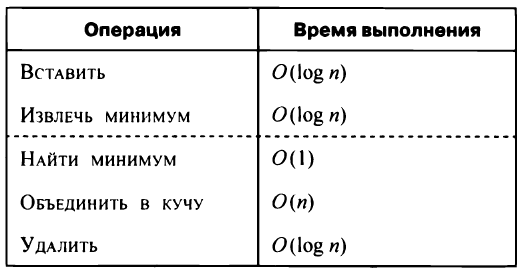
\includegraphics[scale=0.85]{figures/heap.png}
	\caption{ Операции и время их выполнения, поддерживаемые кучами: где $ n $ -- это число объектов, хранящихся в куче }\label{fig:heap}
\end{figure}

\paragraph{Когда использовать кучу} Если приложению требуются быстрые вычисления минимума (либо максимума) для динамически изменяющегося множества объектов, куча обычно является предпочтительной структурой данных.

\paragraph{Кучи в виде дерева} Кучи можно рассматривать как корневое бинарное дерево. Если число хранимых объектов на один меньше степени 2 (например, $ 15 = 2^4 - 1 $), то каждый уровень является \emph{полным}. Когда число объектов находится между двумя такими числами, то единственный неполный уровень является последним, который заполняется слева направо.

ВАЖНО: Бинарное дерево называют \emph{полным}, если каждый его узел либо представляет собой лист, либо имеет строго два дочерних узла. Узлы только с одним дочерним узлом в полном бинарном дереве отсутствуют. Следовательно, порядок дочерних узлов сохраняет информацию о местоположении.

\emph{Свойство кучи}: для каждого объекта $ x $ ключ объекта $ x $ меньше или равен ключам его потомков \pic{fig:heap_tree}.

\begin{figure}[h]
	\centering
	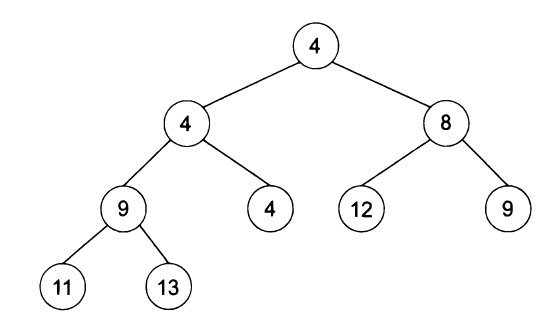
\includegraphics[scale=0.65]{figures/heap_tree.png}
	\caption{ Пример кучи в виде дерева с 9 объектами }\label{fig:heap_tree}
\end{figure}

Для каждой пары <<родитель -- потомок>> ключ родителя не больше ключа потомка. По мере обхода кучи вверх, ключи будут только уменьшаться. При этом корневой ключ является настолько малым, насколько это может получиться. Это должно звучать обнадеживающе, учитывая, что \emph{\color{blue}смысл существования кучи -- быстрые вычисления минимума}.

\paragraph{Кучи в виде массива} Мысленно мы визуализируем кучу как дерево, но в реализации мы используем массив с длинной, равной максимальному числу объектов, которые мы намерены хранить. Первый элемент массива соответствует корню дерева, последующие два элемента -- следующему уровню дерева (в том же порядке), и так далее \pic{fig:heap_tree_array}.

\begin{figure}[h]
	\centering
	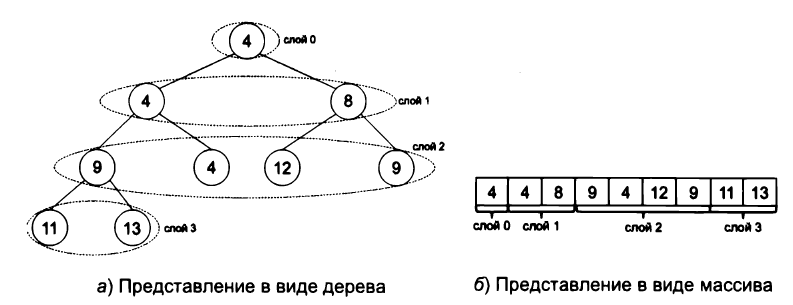
\includegraphics[scale=0.85]{figures/heap_tree_array.png}
	\caption{ Отображение древовидного представления кучи на его представление в виде массива }\label{fig:heap_tree_array}
\end{figure}

Для некорневого объекта (в позиции $ i \geqslant 2 $) родителем $ i $ является объект в позиции $ \lfloor i/2 \rfloor $ (\pic{fig:heap_pos}).

\begin{figure}[h]
	\centering
	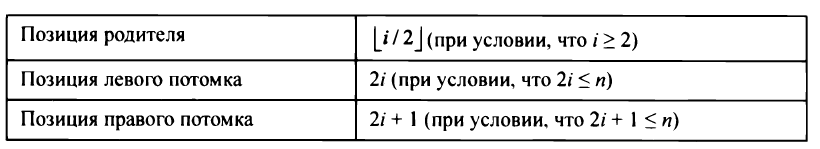
\includegraphics[scale=0.85]{figures/heap_pos.png}
	\caption{ взаимосвязи между позицией $ i \in \{ 1, 2, \ldots, n \} $ объекта в куче и позициями его родителя, левого и правого потомка; $ n $ обозначает число объектов в куче }\label{fig:heap_pos}
\end{figure}

Такие простые формулы для перехода от потомка к его родителю и обратно существуют потому, что мы используем только \emph{полные} бинарные деревья.

В общем случае операция \textsf{Вставить} присоединяет новый объект в конец кучи и многократно переставляет местами узлы нарушающие пары. В любой момент времени существует не более одной нарушающей пары <<родитель -- потомок>> -- пары, в которой новый объект является потомком.

Поскольку куча является полным бинарным деревом, она имеет $ \approx \log_2 n $ уровней, где $ n $ -- число объектов в куче. Число перестановок местами не превышает число уровней, и на перестановку требуется только постоянный объем работ. Таким образом, можно заключить, что в худшем случае время выполнения операции \textsf{Вставить} равно $ O(\log n) $.

Так как операция \textsf{Извлечь минимум} предполагает удаление объекта с наименьшим ключом из кучи и возвращение этого объекта, то корень кучи гарантированно будет таким объектом. Задача заключается в восстановлении \emph{полного бинарного дерева} и свойств кучи после \underline{удаления} корня кучи.

В общем случае операция \textsf{Извлечь минимум} перемещает последний объект кучи в корневой узел (перезаписывая предыдущий корень) и повторно переставляя местами этот объект с его меньшим потомком. В любой момент времени существует не более двух нарушающих пар <<родитель -- потомок>> -- двух пар, в которых ранее последний объект является родителем. 

Число перестановок не превышает число уровней, и на каждую перестановку требуется только постоянный объем работы. Поскольку существует $ \approx \log_2 n $ уровней, мы заключаем, что время выполнения операции \textsf{Извлечь минимум} в худшем случае равно $ O(\log n) $, где $ n $ -- это число объектов в куче.


\subsection{Стеки и очереди}

Стек -- последовательный контейнер, обеспечивающий вставку элемента в вершину стека и удаление элемента из вершины стека.

Очередь -- последовательный контейнер, обеспечивающий добавление элементов в конец очереди и извлечение элементов с начала очереди.

Стеки и очереди представляют собой динамические множества, элементы из которых удаляются с помощью предварительно определенной операции Delete. Первым из \emph{стека} (stack) удаляется элемент, который был помещен туда последним: в стеке реализуется стратегия <<последним пришел -- первым ушел>>\footnote{Стопка тарелок} (last-in, first-out -- LIFO). Аналогично в \emph{очереди} (queue) всегда удаляется элемент, котрый содержится в множестве дольше других: в очереди реализуется стратегия <<превым пришел -- первым ушел>>\footnote{Обычная очередь в магазине} (first-in, first-out -- FIFO) \cite[264]{cormen-algo:2013}.

Операция вставки Insert применительно к стекам часто называется записью в стек Push, а операция удаления Delete, которая вызывается без передачи аргумента, -- снятием со стека Pop.

Применительно к очередям операция вставки называется Enqueue (поместить в очередь), а операция удаления -- Dequeue (вывести из очереди). 

\subsection{Деревья поиска}

\emph{Сбалансированное дерево поиска} (то есть дерево поиска, глубина которого всегда $ O(\log n) $, где $ n $ -- число объектов в дереве) расширяет функционал упорядоченного массива операциями вставки и удаления за логарифмическое время.

\emph{Дерево поиска}, как и куча, представляет собой структуру данных для хранения эволюционирующего множества объектов, ассоциированных с ключами (и, возможно, с большим количеством других данных). Она поддерживает полное упорядочивание хранимых объектов и может поддерживать более богатое множество операций, несколько более медленного времени выполнения.

Использование упорядоченных массивов становится гораздо менее эффективным при частых изменениях базовой коллекции. Поиск на основе хеша может работать с динамическими коллекциями, но с целью эффективного использования ресурсов мы можем выбрать размер хеш-таблицы, который окажется слишком мал; зачастую у нас нет априорного знания о количестве элементов, которые будут храниться в таблице, так что \emph{\color{red}выбрать правильный размер хеш-таблицы оказывается очень трудной задачей}. Кроме того, хеш-таблицы не позволяют обходить все элементы в порядке сортировки \cite[\strbook{150}]{heineman:2017}.

Наиболее распространенным типом дерева поиска является \emph{бинарное дерево поиска} (Binary Search Tree -- BST) (\pic{fig:BST}).

\begin{figure}[h]
	\centering
	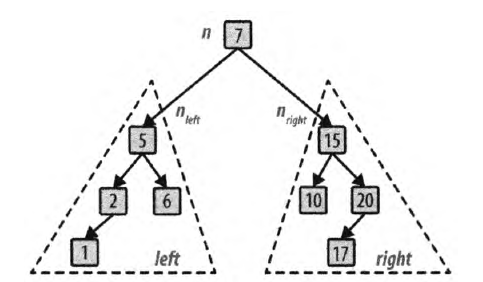
\includegraphics[scale=0.65]{figures/BST.png}
	\caption{ Простое бинарное дерево поиска }\label{fig:BST}
\end{figure}


Неплохая идея представлять \emph{дерево поиска} как динамическую версию \emph{отсортированного массива} -- оно может делать то же, что и отсортированный массив, а также способно быстро производить операции вставки и удаления.

Поддерживаемые операции и их время выполнения в отсортированных массивах приведены на \pic{fig:tree_search}. Смысл \emph{\color{blue}дерева поиска} заключается в поддержке всех операций, поддерживаемых \emph{\color{blue}отсортированным массивом}, а также \emph{вставок} и \emph{удалений}.

\begin{figure}[h]
	\centering
	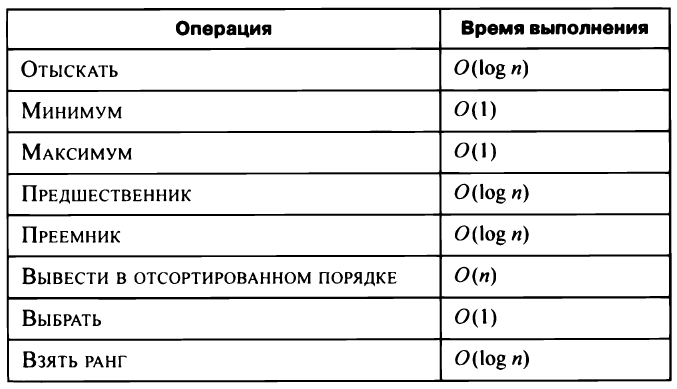
\includegraphics[scale=0.65]{figures/tree_search.png}
	\caption{ Отсортированные массивы: $ n $ -- текущее число объектов в массиве }\label{fig:tree_search}
\end{figure}

На \pic{fig:tree_search_sorted_array} приведен перечень показателей для деревьев поиска в сравнении с отсортированными массивами.

\begin{figure}[h]
	\centering
	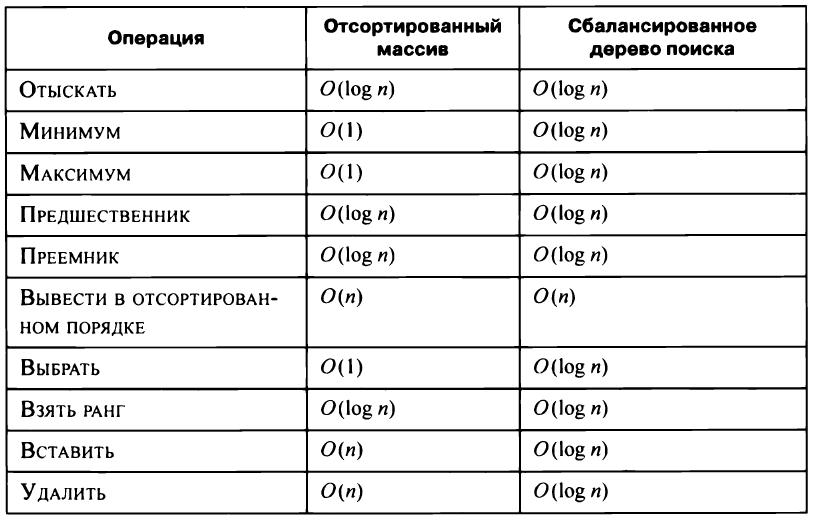
\includegraphics[scale=0.65]{figures/tree_search_sorted_array.png}
	\caption{ \emph{Сбалансированные} деревья поиска и отсортированные массивы: $ n $ -- текущее число объектов в структуре данных }\label{fig:tree_search_sorted_array}
\end{figure}

Важный нюанс: время выполнения на \pic{fig:tree_search_sorted_array} достигается только \emph{сбалансированным} деревом поиска, то есть \underline{более сложной} версией \emph{стандартного бинарного дерева поиска}. Несбалансированное дерево поиска не гарантирует такое время выполнения.

\emph{Сбалансированное дерево поиска} -- дерево поиска, высота которого всегда равна $ O(\log n) $.

\paragraph{Когда использовать сбалансированное дерево поиска} Если приложение нуждается в поддрежке \emph{упорядоченного} представления (функционал отсортированного массива) \emph{динамически изменяющегося множества объектов} (дополнительные операции \underline{удаления} и \underline{вставки}), то сбалансированное дерево поиска (или структура на его основе) обычно является предпочтительной структурой данных.

Если обобщить бинарное дерево поиска имеет смысл использовать, когда \cite[\strbook{151}]{heineman:2017}:
\begin{itemize}
	\item требуется обход данных в возрастающем (или убывающем) порядке,
	
	\item размер множества данных неизвестен, а реализация должна быть в состоянии обработать любой возможный размер, помещающийся в памяти,
	
	\item множество данных -- динамическое, с большим количеством вставок и удалений в процессе работы программы.
\end{itemize}

ВАЖНО: В худшем случае бинарное дерево поиска может выродиться и превратиться в связанный список. Для сохранения оптимальной производительности необходимо балансировать BST после каждого добавления (и удаления).

Если нужно поддерживать только \emph{упорядоченное} представление, но \underline{статической} совокупности данных (без вставок и удалений), то имеет смысл использовать вместо сбалансированного дерева поиска \emph{отсортированный массив}. Если набор данных является динамическим, но вас интересуют только быстрые операция взятия \emph{минимума} (либо \emph{максимума}), то вместо сбалансированного дерева поиска используйте \emph{кучи}. 

AVL-деревья (деревья Адельсона-Вельского-Ландиса) -- это самобалансирующиеся бинарные деревья поиска. Давайте определим понятие высоты AVL-узла. Высота листа равна 0, потому что он не имеет дочерних элементов. Высота узла, не являющегося листом, на 1 больше максимального значения высоты двух его дочерних узлов. Для обеспечения согласованности высоты несуществующего дочернего узла считается равной -1.

AVL-дерево гарантирует AVL-свойство для каждого узла, заключающееся в том, что разница высот для любого узла равна -1, 0 или 1. Разница высот определяется как $ height(left) - height(right) $, т.е. высота левого поддерева минус высота правого поддерева. AVL-дерево должно обеспечивать выполнение этого свойства всякий раз при вставке значения в дерево или удалении из него. 

\paragraph{Детали реализации} (здесь описывается типичная реализация не обязательно сбалансированного бинарного дерева поиска) В бинарном дереве поиска каждый узел соответствует объекту (с ключом) и имеет три ассоциированных с ним указателя: указатель на родителя, указатель на левого потомка и указатель на правого потомка. Любой из этих указателей может быть пустым, то есть иметь значение null, указывающее на отстутствие родителя или потомка. 

\emph{Свойство дерева поиска}:
\begin{itemize}
	\item Для каждого объекта $ x $ объекты в левом поддереве объекта $ x $ имеют ключи меньше, чем у $ x $,
	
	\item Для каждого объекта $ x $ объекты в правом поддереве объекта $ x $ имеют ключи больше, чем у $ x $.
\end{itemize}

Другими словами, значения ключа левого дочернего узла меньше значения ключа родительского узла, а значение ключа правого дочернего узла больше значения ключа родительского узла и, как следствие, ключи дочерних узлов упорядочены слева направо.

Свойство дерева поиска накладывает требование на каждый узел дерева поиска, а не только на корень (\pic{fig:tree_search_schema1}).

\begin{figure}[h]
	\centering
	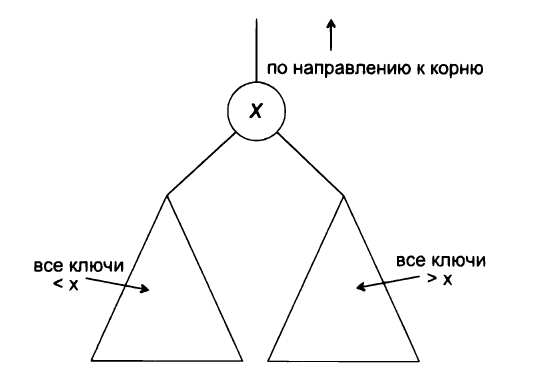
\includegraphics[scale=0.85]{figures/tree_search_schema1.png}
	\caption{ Дерево поиска }\label{fig:tree_search_schema1}
\end{figure}

Например, покажем дерево поиска, содержащее объекты с ключами $ \{ 1, 2, 3, 4, 5 \} $, и таблицу, перечисляющую места назначения трех указателей в каждом узле (\pic{fig:tree_search_schema2})

\begin{figure}[h]
	\centering
	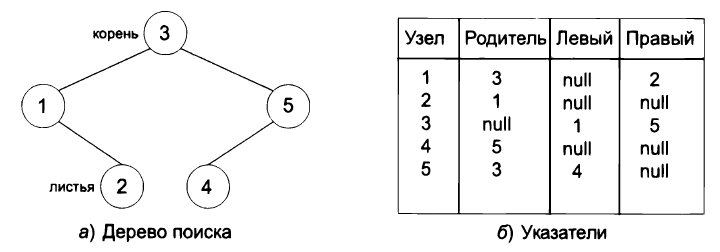
\includegraphics[scale=0.85]{figures/tree_search_schema2.png}
	\caption{ Дерево поиска и соответствующие ему указатели на родителя и потомков }\label{fig:tree_search_schema2}
\end{figure}

Бинарные деревья поиска и кучи различаются по нескольким направлениям. Кучи можно рассматривать как деревья, но реализованы они как массивы, без явных указателей между объектами. Дерево поиска явным образом хранит тре указателя в расчете на объект и, следовательно, использует больше места (с постоянным множителем).

\emph{\color{blue}Кучам} явные указатели не нужны, потому что они \underline{\color{blue}всегда} соответствуют \emph{\color{blue}полным бинарным деревьям}, в то время как \emph{бинарные деревья поиска} могут иметь \emph{произвольную структуру}.

Деревья поиска имеют иное предназначение, чем кучи. По этой причине свойство дерева поиска несопоставимо со свойством кучи. \emph{Кучи} оптимизированы для вычислений \emph{минимума}, а свойство кучи -- то, что ключ потомка больше только ключа родителя, -- упрощает поиск объекта с минимальным ключом (\emph{это корень}). \emph{\color{blue}Деревья поиска} оптимизированы, как ни странно, для \emph{\color{blue}поиска}, и свойство дерева поиска определено соответствующим образом.

Например, если вы ищете объект с ключом 23 в дереве поиска и ключом корня является 17, то вы знаете, что объект может располагаться только в правом поддереве корня, и можете исключить объекты в левом поддереве из дальнейшего рассмотрения. Это должно напоминать о бинарном поиске, как и подобает структуре данных, смысл которой заключается в симулировании динамически изменяющегося отсортированного массива.

\paragraph{Высота дерева поиска} Для заданного множества ключей существует множество разных деревьев поиска. Высота дерева определяется как длина самого длинного пути от корня до листа (ее еще называют глубиной). В общем случае \emph{бинарное дерево поиска}, содержащее $ n $ объектов, может иметь какую угодно глубину от $ \approx \log_2 n $ (идеально сбалансированное бинарное дерево\footnote{Наилучший вариант}) до $ n - 1 $ (цепочка\footnote{Наихудший вариант}).

\paragraph{Реализация операции Отыскать со временем $ O(\text{высота}) $} Отыскать означает по ключу $ k $ вернуть указатель на объект в структуре данных с ключом $ k $ (либо сообщить, что такого объекта не существует). Свойство дерева поиска указывает, где именно искать объект с ключом $ k $. Если $ k $ меньше (либо, соответственно, больше) ключа корня, то такой объект должен располагаться в левом поддереве (в правом поддереве соответственно) корня. 

Время выполнения пропорционально количеству пройденных указателей, которое не превышает глубину дерева поиска.

\paragraph{Реализация операций Минимум и Максимум за время $ O(\text{высота}) $} Ключи в левом поддереве корня могут быть только меньше ключа корня, и ключи в правом поддереве могут быть только больше. Если левое поддерево является пустым, то корень должен быть минимальным. В противном случае минимум левого поддерева также является минимумов всего дерева. Это наводит на мысль о том, чтобы следовать по указателю на левого потомка корня и повторять данный процесс.

Время работы пропорционально числу пройденных указателей, которое равно $ O(\text{высота}) $.

\paragraph{Сбалансированные деревья поиска} Во всех наиболее распространенных реализациях сбалансированных деревьях поиска используются \emph{повороты} -- операции с постоянным временем, выполняющие небольшую локальную перебалансировку при сохранении свойства дерева поиска.


\subsection{Массивы и связанные списки}

Связанный список (linked list) -- это структура данных, в которой объекты расположены в линейном порядке. Однако, в отличие от массива, в котором этот порядок определен индексами, порядок в связанном списке определяется указателями на каждый объект.

\emph{\color{blue}Массивы} чрезвычайно полезны из-за того, что они поддерживают \emph{\color{blue}произвольный доступ}, то есть другими словами \emph{чтение элемента} в массиве выполняется за \emph{постоянное время} $ O(1) $.

Всего существует два вида доступа:
\begin{itemize}
	\item \emph{произвольный},
	
	\item \emph{последовательный}.
\end{itemize}

При последовательном доступе элементы читаются по одному, начиная с первого. \emph{\color{blue}Связанные списки} поддерживают только \emph{\color{blue}последовательный} доступ. Если требуется прочитать 10-ый элемент связанного списка, то придется прочитать первые 9 элементов и перейти по ссылкам к 10-ому элементу.

Вставка и удаление выполняются за постоянное время $ O(1) $ только в том случае, если доступ к элементу можно получить мгновенно. Для удаления элемента лучше подходит связанный список, потому что в нем достаточно изменить указатель в предыдущем элементе, а в массиве при удалении элемента все последующие элементы нужно будет сдвинуть вверх.


\subsection{В-деревья}

\emph{B-деревья} представляют собой \emph{сбалансированные деревья поиска}, созданные специально для эффективной работы с дисковой памятью (и другими типами вторичной памяти с непосредственным доступом). Многие СУБД используют для хранения информации именно B-деревья или их разновидности.

B-деревья отличаются от красно-черных деревьев тем, что узлы B-дерева могут иметь много дочерних узлов -- от нескольких штук до тысяч, так что степень ветвления B-дерева может быть очень большой (хотя обычно она определяется характеристиками используемых дисков). B-деревья схожи с красно-черными деревьями в том, что все В-деревья с $ n $ узлами имеют высоту $ O(\lg n) $, хотя само значение высоты В-дерева существенно меньше, чем у красно-черного дерева за счет более сильного ветвления. Таким образом, В-деревья также могут использоваться для реализации многих операций над динамическими множествами за время $ O(\lg n) $ \cite[\strbook{521}]{cormen-algo:2013}.

В-деревья представляют собой естественное обобщение бинарных деревьев поиска.


\section{Элементы теории графов}

Под \emph{инвариантом} молекулярного графа подразумевают такую величину, которая принимает одно и то же численное значение при любой произвольной нумерации вершин графа. Инварианты молекулярных графов получили в литературе название \emph{топологических индексов}.  

В \cite{farrel-combinatorial-theory:1979} дается дословно следующее определение парасочетания: <<Под паросочетанием $ M $ графа $ G $ мы будем понимать основной подграф графа $ G $, состоящий только из ребер и вершин. Если $ M $ содержит $ k $ ребер, то $ M $ называется $ k $-парасочетанием. Ясно, что если $ G $ содержит $ p $ вершин, то $ k $-паросочетание в $ G $ содержит $ p - 2k $ вершин>>. И далее следует формула для полинома паросочетаний
\begin{align}\label{eq:kparosochet}
	M(G, w) = \sum_{k = 0}^{ [ p/2 ]} a_k w_1^{p - 2k} w_2^k,
\end{align}
где $ p $ -- число вершин графа $ G, $ $ w = (w_1, w_2) $ -- весовой 2-вектор, компоненты которого образуют полином, $ w_1 $ -- вес вершин, $ w_2 $ -- вес ребер, $ a_k $ -- число $ k $-паросочетаний.

В формуле \eqref{eq:kparosochet} число $ k $-паросочетаний трактуется как $ k $ попарно не связанных ребер.

В работе \cite{kruglyak-new-invar:2015} предлагается считать, что веса ребер $ w_2 $ в формуле \eqref{eq:kparosochet} не равны между собой, а характеризуют химическую связь, соответствующую данному ребру. И тогда для каждого паросочетания $ M_k^j $ вместо $ w_2^k $ можно записать $ \prod_{i=1}^{k}b_i^j $, где $ b_i^j $ -- вес $ i $-ого ребра, принадлежащего $ j $-му $ k $-паросочетанию $ M_k^j $. Аналогично раскрывается $ w_1^{p-2k} $ в \ref{eq:kparosochet}. Если считать различными веса вершин, то $ w_1^{p-2k} $ преобразуется $ \prod_{i=1}^{p - 2k} a_i^j$, где $ a_i^j $ принадлежат $ M_k^j $. В результате каждому $ k $-паросочетанию соответствует произведение весов входящих в него вершин и ребер, и число таких произведений равно $ P(G, k) $. В итоге получим \cite{kruglyak-new-invar:2015}
\begin{align}\label{eq:p_tilde}
	\tilde{P}(G, k) = \sum_{j=1}^{P(G, k)} \Bigg( \prod_{i=1}^{p - 2k} a_i^j \prod_{i=1}^{k} b_i^j \Bigg).
\end{align}

Отсюда легко получается \emph{индекс паросочетаний} предлагаемый в работе \cite{kruglyak-new-invar:2015}
\begin{align*}
	R(G) = \sum_{k=1}^{[p/2]} \tilde{P}(G, k)
\end{align*}

Числа $ \tilde{P}(G, k) $ можно называть значениями $ k $-гетеропаросочетаний и использовать их в соответствующих полиномах вместо $ P(G, k) $. В случае если веса вершин и ребер равны единице, то $ \tilde{P}(G, k) = P(G, k) $, и предлагаемый индекс паросочетаний \eqref{eq:p_tilde} превращается в индекс Хосойи\footnote{Еще говорят топологический индекс Хосойи}. Отличие предлагаемого в работе \cite{kruglyak-new-invar:2015} метода построения индекса паросочетаний от использовавшихся подходов ранее заключается в том, что при суммировании по подграфам в каждом слагаемом участвуют как характеристики элементов этих подграфов (в данном случае ребер), так и характеристики непокрываемых этими подграфами вершин, что позволяет в каждом слагаемом учесть влияние окружения.

В работе \cite{kruglyak-new-invar:2015} сформулирован общий принцип построения топологических инвариантов взвешенных графов для корреляции <<структура-свойство>>, а именно
\begin{align*}
	I(G) = \sum_{G_i} \prod_{j \in E_i} b_j \prod_{k \in V^{'}_i} a_k,
\end{align*}
где $ G_i $ -- всевозможные подграфы графы $ G $ заданного вида, $ E_i $ -- множество ребер с весами $ b_j $ этих подграфов, $ V^{'}_i $ -- множество вершин с весами $ a_k $ подграфов $ G^{'}_i G \setminus G_i $.

\subsection{Инварианты на графах}

В качестве инварианта графа можно рассматривать не какое-то отдельно взятое значение инварианта, а их кортеж (супериндекс) вида $ (p_0, p_1, \ldots) $.

Инвариант называется \emph{полным}, если для установления изоморфизма двух графов с помощью рассматриваемого инварианта необходимо и достаточно, чтобы инвариант возвращал на этих графах одно и тоже значение.

В изоморфных графах инварианты совпадают, но обратное неверно. То есть равенство инвариантов у двух графов не гарантирует их изоморфизма.

\emph{Индекс Хосойи графа} это полное число паросочетаний\footnote{Паросочетание (независимое множество ребер на графе) -- это набор попарно несмежных ребер, то есть ребер, не имеющих общих вершин} на графе. Индекс Хосойи всегда $ \geqslant 1 $, поскольку пустое множество ребер рассматривается как паросочетание. Например, путь с одним ребром имеет два паросочетания (одно -- с пустым набором ребер, а другое с одним ребром), так что его индекс Хосойи равен 2.

\emph{Индекс Винера} -- топологический индекс неориентированного графа, определяемый как сумма длин кратчайших путей $ d(v_i, v_j) $ между вершинами графа
\begin{align*}
	W(G) = \sum_{\forall i, j} d(v_i, v_j).
\end{align*}

Может быть вычислен с использованием алгоритма Флойда-Уоршелла за время порядка $ O(n^3) $.

\emph{Индекс Рандича} (индекс связности) -- индекс неориентированного графа
\begin{align*}
	r = \sum_{(v_i, v_j) \in V} \dfrac{1}{ \sqrt{d(v_i)d(v_j)} },
\end{align*}
где $ v_{i, j} $ -- вершины образующие ребро\footnote{То есть рассматривать следует не все возможные сочетания пар вершин, а только те, которые образуют ребро}, $ d(v_k) $ -- степень вершины\footnote{Степерь вершины графа -- число ребер графа, которым принадлежит эта вершина. Вершина называется четной, если ее степень -- число нечетное} $ v_k $.


\section{Площадь под ROC-кривой}

Площадь под ROC-кривой (\href{https://dyakonov.org/2017/07/28/auc-roc-площадь-под-кривой-ошибок/}{ROC AUC}) можно вычислить так
\begin{align*}
	ROC AUC = \dfrac{ \sum\limits_{i=1}^{q}\sum\limits_{j=1}^{q} I[y_i < y_j] I^{'}[a_i < a_j]}{ \sum\limits_{i=1}^{q}\sum\limits_{j=1}^{q} I[y_i < y_j] },
\end{align*}
\vspace*{-5mm}
\begin{align*}
	I^{'}[a_i < a_j] =
	    \begin{cases}
		    0, &a_i > a_j,\\
		    1/2, &a_i = a_j,\\
		    1, &a_i < a_j.
		\end{cases}, \quad I[y_i < y_j] = 
	        \begin{cases}
	        	0, &y_i \geqslant y_j,\\
	        	1, &y_i < y_j,
	        \end{cases}
\end{align*}
где $ a_i $ -- ответ классификатора на $ i $-ом экземпляре, $ y_i $ -- метка класса на $ i $-ом экземпляре, $ q $ -- число экземпляров тестового набора данных.

ВАЖНО: Таким образом, ROC AUC это доля пар экземпляров вида <<экземпляр положительного класса, экземпляр отрицательного класса>>, которые алгоритм верно упорядочил.

\paragraph{Вероятностная интерпретация ROC AUC} Пуcть алгоритм (классификатор) возвращает некоторую \emph{оценку принадлежности экземпляра к положительному классу} (это может быть \emph{вероятность} принадлежности экземпляра к положительному классу, но не обязательно). Можно считать, что эта оценка принимает значения из отрезка $ [0;1] $.

ВАЖНО: В этом случае \emph{площадь под ROC-кривой} это вероятность события, состоящего в том, что классификатор на случайно выбранном экземпляре положительного класса вернет оценку принадлежности экземпляра к положительному классу выше, чем на экземпляре отрицательного класса, т.е.
\begin{align*}
	ROC AUC = \mathbf{P} \Big( a(x_i) < a(x_j) \, | \, y_i = 0, y_j = 1\Big).
\end{align*}


\section{NP-полнота}

\subsection{Краткая сводка}

\emph{Полиномиальные алгоритмы} -- алгоритмы, время работы которых на входе длины $ n $ в наихудшем случае равно $ O(n^k) $ для некоторой константы $ k $ (не зависящей от длины входа). Вообще говоря, о задачах, разрешимых с помощью алгоритмов с полиномиальным временем работы, возникает представление как о легко разрешимых или простых, а о задачах, время работы которых превосходит полиномиальное время, -- как о трудно разрешимых или сложных \cite[1096]{cormen-algo:2013}.

\emph{P-задачей} (полиномиальной задачей) называется задача, которую \emph{можно решить} за полиномиальное (от длинны входа) время. Точнее говоря, это задачи, которые можно решить за время $ O(n^k) $, где $ k $ -- некоторая константа, а $ n $ -- размер входных данных задачи.

\emph{NP-задачей} (недетирминированно полиномиальной задачей) называется задача, которую можно решить только на \emph{недетерминированной машине}\footnote{В недетерминированных машиных следующее состояние не всегда однозначно определяется предыдущим. Работу такой машины можно представить как разветвляющийся на каждой неоднозначности процесс: задача считается решенной, если хотя бы одна ветвь процесса пришла к ответу} Тьюринга за \emph{полиномиальное} время. Другими словами, класс NP состоит из задач, которые поддаются \emph{проверке} в течение полиномиального времени. Имеется в виду, что если мы каким-то образом получаем <<сертификат>> решения, то в течение времени, полиномиальным образом зависящего от размера входных данных задачи, можно проверить корректность такого решения.

Задача называется \emph{NP-полной}, если для нее не существует эффективных алгоритмов решения и к этой задаче можно свести любую другую задачу из класса NP за полиномиальное время. Таким образом, {\color{blue}\itshape NP-полные задачи образуют в некотором смысле подмножество <<самых сложных>> задач в классе NP}. И если для какой-то из них будет найден <<быстрый>> алгоритм решения, то и любая другая задача из класса NP может быть решена так же <<быстро>>.

\emph{Сводимость по Карпу}. Задача разрешения $ P_1 $ полиномиально сводится к задаче разрешения $ P_2 $, если
\begin{itemize}
	\item существует полиномиально вычислимая функция $ f: I_1 \to I_2 $ (отображает входные данные $ I_1 $ для $ P_1 $ во входные данные $ I_2 \equiv f(I_1) $ для задачи $ P_2 $),
	
	\item $ \forall I_1 $ совпадают ответы на вопросы <<$ P_1(I_1) $?>> и <<$ P_2(f(I_1)) $?>>.
\end{itemize} 

ВАЖНО: NP-полные задачи это задачи, для которых не доказано ни то, что они не могут быть решены за полиномиальное время, ни то, что 

ВАЖНО: Никакую NP-полную задачу нельзя решить никаким известным алгоритмом полиномиальной сложности.

На \pic{fig:np} изображена диаграмме Венна взаимоотношений между классами $ P $, $ NP $, $ NP $-полными и $ NP $-трудными в случае если $ P \neq NP $.

\begin{figure}[h]
	\centering
	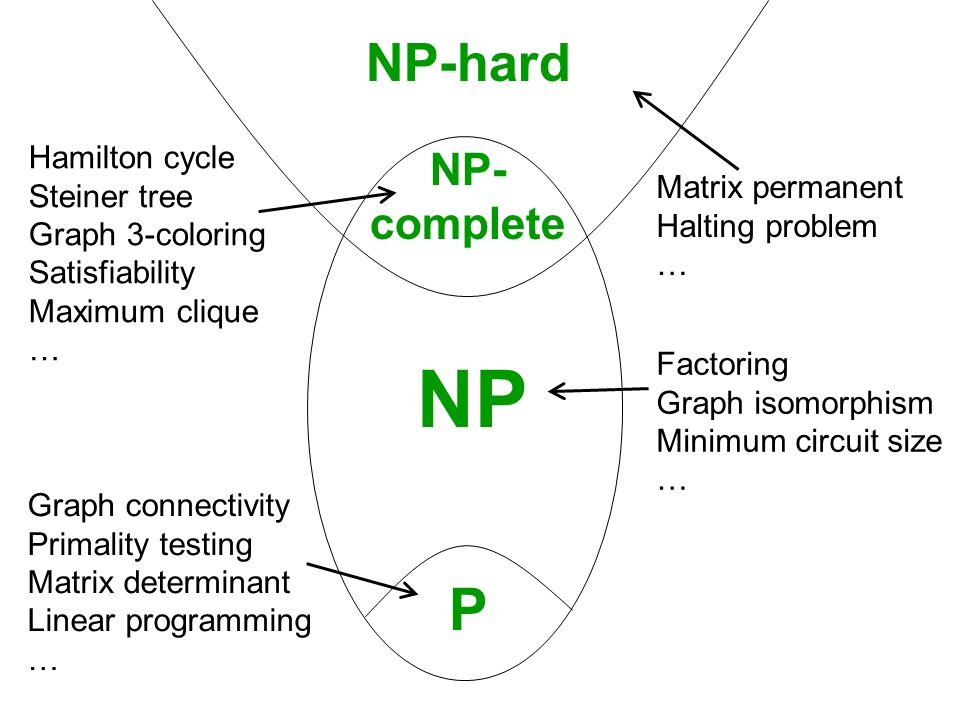
\includegraphics[scale=0.35]{figures/np.jpg}
	\caption{ Диаграмма Венна взаимоотношений между классами P, NP, NP-полными и NP-трудными }\label{fig:np}
\end{figure}

ВАЖНО: недетерминированность проще всего понять, рассматривая алгоритм, который производит вычисления до тех пор, пока не доходит до места, в котором должен быть сделан выбор из нескольких альтернатив. Детерминированный алгоритм исследовал бы сначала одну альтернативу, а потом вернулся бы для рассмотрения следующей альтернативы. \emph{Недетерминированный} алгоритм может исследовать все альтернативы \emph{одновременно}, по сути <<копируя>> самого себя для каждой альтернативы. Все копии работают независимо. Если копия обнаруживает, что данный путь безрезультатный, то она прекращает выполняться. Если копия находит требуемое решение, она объявляет об этом, и все копии прекращают работать. Детерминированная машина Тьюринга является частным случаем недетерминированной машины Тьюринга и не имеет копий.

Нахождение алгоритма, решающего какую-либо NP-полную задачу за полиномиальное время, позволит найти решение NP-задач за полиномиальное время, то есть позволит считать их P-задачами.

Трудоемкость более сложных задач растет экспоненциально с увеличением объема данных. Алгоритмы с экспоненциальным временем считаются неэффективными. 

Если для какой-то NP-полной задачи найден полиномиальный алгоритм решения, то и любая другая задача из класса NP может быть решена за полиномиальное время.

Если установлено, что задача NP-полная, это служит достаточно надежным указанием на то, что она \emph{трудноразрешимая} \cite[1088]{cormen-algo:2013}.

Для демонстрации сложности задач с помощью сведений нужно начать с одной \emph{заведомо сложной задачи}. {\color{red}Самой сложной изо всех \emph{NP-полных} задач} является логическая задача, называющаяся \emph{задачей выполнимости ({\rmfamily satisfiability}) булевых формул} \cite[351]{skiena-algo:2011}.

Экземпляром задачи SAT является булева формула, состоящая только из имен переменных, скобок и операций И, ИЛИ и НЕ. Согласно теореме Кука, задача SAT для булевых формул, записанных в \emph{конъюктивной нормальной форме}, является \emph{NP-полной}. Требование к записи в конъюктивной нормальной форме существенно, так как, например, задача SAT для формул, представленных в дизъюктивной нормальной форме, тривиально решается за линейное время в зависимости от размера записи формулы.

Если известно эффективное решение задачи SAT, то можно эффективно решить любую задачу в классе NP. Иначе говоря, SAT -- это задача-представитель класса, она является <<сложнейшей>> в своем классе и позволяет решить все другие задачи в NP.

ВАЖНО: вопрос о том, будет ли $ P = NP $ является открытой проблемой теории сложности. Широко распространено мнение, что $ P \neq NP $, а следовательно $ P \subset NP $.

\subsection{Интуитивное определение SAT, NP и P}

Формула $ F $ -- это синтаксически правильный набор переменных и коннекторов, т.е. \emph{следствие}, \emph{И}, \emph{ИЛИ} соединяют переменные или другие формулы, а \emph{НЕ} стоит перед переменной или формулой. Пример $ F = (x \rightarrow (y \ OR \ z)) \ AND \ (x \rightarrow NOT \ x) $.

Говорят, что формула $ F $ выполнима (SAT) тогда и только тогда (далее для краткости iff -- if and only if), если ее переменным можно приписать значения Истина/Ложь, таким образом, что $ F $ истина.

Любая пропозиционная формула $ F $ может быть приведена к виду CNF (Conjunctive Normal Form), т.е. быть представлена в виде
\begin{align*}
	F' = c_1 \ AND \ c_2 \ AND \ \ldots \ c_n,
\end{align*}
где $ c_i $ -- это $ x \ OR \ y \ OR \ z $, а $ x, y, z $ -- это переменные или их отрицания.

Пример
\begin{align*}
	F = (x \ OR \ NOT y \ OR \ NOT z) \ AND \ (NOT x \ OR \ NOT y \ OR \ h) \ AND \ (z \ OR \ h).
\end{align*}

Чтобы каждое предложение содержало не более трех переменных, потребуется ввести дополнительные переменные, но это исключительно технические детали.

В таком виде, когда формула имеет вид описанный выше задачи носит название 3-SAT, подчеркивая тот факт, что каждое предложение $ c_i $ содержит не более трех переменных или их отрицаний.

\paragraph{класс P} (он же класс PTIME) -- задачи разрешимые за \emph{полиномиальное} время. Это значит, что число шагов алгоритма в данном классе растет не более, чем некотрый полином от входных данных.

Входным параметром является массив чисел для сортировки. Нас интересует рост времени в зависимости от роста длины массива, т.е. зависимость времени TIME (оно количество операций) от $ n $. 

В сортировке пузырьком количество операций (TIME) растет как квадрат от длины массива, т.е. $ TIME(n) = a n^2 + b n + C $. В данном случае \emph{время работы алгоритма} растет не быстрее квадрата числа элементов и записывается это как $ TIME(n) \in O(n^2) $.

\paragraph{класс NP} обозначает класс недетерминированн полиномиальное время. Сама природа и внутренние механизмы NP следуют так называемому guess-and-check подходу (угадать и проверить). Пространство поиска решений экспоненциально (достаточно большое, чтобы исключить возможность перебора), а проверка решения является простой задачей. Можно рассматривать NP, как класс задач, в котором нужно найти решение (guess часть) среди большого количества вариантов, а потом проверить его корректность (check часть).

 С точки зрения SAT, пространство решений это всевозможные наборы значений переменных, если у нас $ k $ различных переменных в формуле, то у нас $ 2^k $ возможных <<интерпретаций>> формулы, т.е. пространство поиска $ I $ экспоненциально. Однако, если мы <<угадали>> $ I $, то мы можем за полиномиальное время проверить истинность формулы.



\section{Настройка непрерывной интеграции (CI) на GitHub Actions}

\subsection{Порядок работы с pull-request}

Кратко о pull-request. Pull-request (запрос на изменения) -- запрос к управляющему каким-либо репозиторием (человеку, группе или вообще роботу) на выполнение изменений из вашего репозитория (и указанной ветки).

Порядок выполнения pull-request на свой проект:
\begin{itemize}
	\item Делаем форк репозитория,
	
	\item Через свой собственный GitHub-профиль клонируем репозиторий на локальную машину,
	
	\item Создаем новую ветку под изменения,
	
	\item Вносим изменения из-под новой ветки,
	
	\item Делаем \texttt{git push origin my\_branch},
	
	\item На странице GitHub репозитория выбираем новую ветку и нажимаем кнопку <<Compare \& pull request>>; появится форма, в которой можно описать коммит и и добавить комментарий; затем нажимаем <<Create pull request>>,
	
	\item На вкладке <<Pull requests>> появится диалоговая форма с возможностью сделать <<Merge pull request>>, просмотреть коммит и пр.
\end{itemize}

Можно выполнить <<Merge pull request>> через командную строку
\begin{lstlisting}[
style = bash,
numbers = none
]
# Step 1: From your project repository, bring in the changes and test.
git fetch origin
git checkout -b correct-description-readme origin/correct-description-readme
git merge main

# Step 2: Merge the changes and update on GitHub.
git checkout main
git merge --no-ff correct-description-readme
git push origin main
\end{lstlisting}

После удачного <<Merge pull request>> лучше удалить соответствующие локальную и удаленную (remote) ветки
\begin{lstlisting}[
style = bash,
numbers = none	
]
# удаление локальной ветки
git branch -d <branch_name>
# удаление удаленной ветки
git push origin --delete <branch_name>
\end{lstlisting}



\subsection{Конфигурационные файлы для непрерывной интеграции}

Существуют различные инструменты непрерывной интеграции (continuous integration, CI). Вот некоторые из них
\begin{itemize}
	\item GitHub CI,
	
	\item CircleCI,
	
	\item Travis CI,
	
	\item Buildkite и т.д.
\end{itemize}

В качестве пример рассмотрим настройку непрерывной интеграции с помощью GitHub Actions.

Простой пример \texttt{ci.yaml} 
\begin{lstlisting}[
title = {\sffamily .github/workflows/ci.yaml},
style = bash,
numbers = none	
]
# This workflow will install Python dependencies, run tests and lint with a variety of Python versions
# For more information see: https://help.github.com/actions/language-and-framework-guides/using-python-with-github-actions

name: Python package

on:
push:
branches: [ master ]
pull_request:
branches: [ master ]
jobs:
build:
runs-on: ubuntu-latest
strategy:
matrix:
python-version: [3.6, 3.7, 3.8]
steps:
- uses: actions/checkout@v2
- name: Set up Python
uses: actions/setup-python@v2
with:
python-version: ${{ matrix.python-version }}
- name: Cache pip
uses: actions/cache@v1
with:
path: ~/.cache/pip # This path is specific to Ubuntu
# Look to see if there is a cache hit for the corresponding requirements file
key: ${{ runner.os }}-pip-${{ hashFiles('requirements.txt') }}
restore-keys: |
${{ runner.os }}-pip-
${{ runner.os }}-
# You can test your matrix by printing the current Python version
- name: Display Python version
run: python -c "import sys; print(sys.version)"
- name: Install dependencies
run: |
python -m pip install --upgrade pip
pip install Cython
pip install -r requirements.txt
pip install pycocotools
pip install shapely
pip install black flake8 mypy pytest hypothesis isort pylint
- name: Run black
run:
black --check .
- name: Run flake8
run: flake8
- name: Run pylint
run: pylint iglovikov_helper_functions
- name: Run Mypy
run: mypy iglovikov_helper_functions
- name: Run isort
run: isort --profile black iglovikov_helper_functions
- name: tests
run: |
pip install .[tests]
pytest
\end{lstlisting}

Пример CI-файла посложнее
\begin{lstlisting}[
title = {\sffamily .github/workflows/ci.yaml},
style = bash,
numbers = none	
]
name: CI
on: [push, pull_request]  # триггеры

jobs:
  test_and_lint:
    name: Test and lint
    runs-on: ${{ matrix.operating-system }}
    strategy:
      matrix:
        operating-system: [ubuntu-latest, windows-latest, macos-latest]
        python-version: [3.6, 3.7, 3.8]
      fail-fast: false
    steps:
    - name: Checkout
      uses: actions/checkout@v2
    - name: Set up Python
      uses: actions/setup-python@v2
      with:
        python-version: ${{ matrix.python-version }}
    - name: Update pip
      run: python -m pip install --upgrade pip
    - name: Install PyTorch on Linux and Windows
      if: >
        matrix.operating-system == 'ubuntu-latest' ||
        matrix.operating-system == 'windows-latest'
      run: >
        pip install torch==1.4.0+cpu torchvision==0.5.0+cpu
        -f https://download.pytorch.org/whl/torch_stable.html
    - name: Install PyTorch on MacOS
      if: matrix.operating-system == 'macos-latest'
      run: pip install torch==1.4.0 torchvision==0.5.0
    - name: Install dependencies
      run: pip install .[tests]
    - name: Install linters
      run: pip install "pydocstyle<4.0.0" flake8 flake8-docstrings mypy
    - name: Run PyTest
      run: pytest
    - name: Run Flake8
      run: flake8
    - name: Run mypy
      run: mypy .

  check_code_formatting:
    name: Check code formatting with Black
    runs-on: ubuntu-latest
    strategy:
      matrix:
        python-version: [3.8]
    steps:
    - name: Checkout
      uses: actions/checkout@v2
    - name: Set up Python
      uses: actions/setup-python@v2
      with:
        python-version: ${{ matrix.python-version }}
    - name: Update pip
      run: python -m pip install --upgrade pip
    - name: Install Black
      run: pip install black==19.3b0
    - name: Run Black
      run: black --config=black.toml --check .

  check_sphinx_build:
    name: Check Sphinx build for docs
    runs-on: ubuntu-latest
    strategy:
      matrix:
        python-version: [3.8]
    steps:
    - name: Checkout
      uses: actions/checkout@v2
    - name: Set up Python
      uses: actions/setup-python@v2
      with:
        python-version: ${{ matrix.python-version }}
    - name: Update pip
      run: python -m pip install --upgrade pip
    - name: Install dependencies
      run: pip install -r docs/requirements.txt
    - name: Run Sphinx
      run: sphinx-build -b html docs /tmp/_docs_build

  check_transforms_docs:
    name: Check that transforms docs are not outdated
    runs-on: ubuntu-latest
      strategy:
        matrix:
          python-version: [3.8]
      steps:
      - name: Checkout
        uses: actions/checkout@v2
      - name: Set up Python
        uses: actions/setup-python@v2
        with:
          python-version: ${{ matrix.python-version }}
      - name: Update pip
        run: python -m pip install --upgrade pip
      - name: Install dependencies
        run: pip install .
      - name: Run checks
        run: python tools/make_transforms_docs.py check README.md
\end{lstlisting}


\section{Настройка непрерывной доставки (CD) с помощью Codefresh}

\section{Разработка собственных Python-пакетов для PyPI}

\subsection{Семантическое управление версиями}

Номер релиза обычно дается в формате \href{https://semver.org/}{MAJOR.MINOR.PATCH}:
\begin{itemize}
	\item MAJOR: изменяется, когда разработчики вносят обратно несовместимые изменения API,
	
	\item MINOR: изменяется, когда разработчики вносят обратно совместимые изменения; например, если какая-нибудь функция публичного API признается устаревшей или появляется обратно совместимая новая функциональность,
	
	\item PATCH: изменяется, когда разработчики исправляют обратно совместимые ошибки (x.y.Z | x > 0).
\end{itemize}

Предрелизная версия имеет более низкий приоритет, чем связанные с ней обычные версии. Предрелизная версия указывает, что версия нестабильна и может не удовлетворять предполагаемым требованиям совместимости. Примеры: \texttt{1.0.0-alpha}, \texttt{1.0.0-alpha.1}, \texttt{1.0.0-0.3.7}.

Можно указывать метаданные сборки (метаданные не входят в приоритет): \texttt{1.0.0-alpha+001}, \texttt{1.0.0+201303}, \texttt{1.0.0-beta+exp.sha.5114f85}.

Пример разрешения приоритетов: \texttt{1.0.0-alpha} < \texttt{1.0.0-alpha.1} < \texttt{1.0.0-alpha.beta} < \texttt{1.0.0-beta} < \texttt{1.0.0-beta.2} < \texttt{1.0.0-beta.11} < \texttt{1.0.0-rc.1} < \texttt{1.0.0}.

\subsection{Краткая дорожная карта разработки собственного пакета}

Дорожная карта по разработке пользовательского python-пакета для PyPI:

\begin{enumerate}
	\item Создать рабочую директорию пакета, например, с именем \texttt{advancedstatistic}: другими словами, это директория локального git-репозитория, в которой будут расположены поддиректории с python-модулями, реализующими основной функционал пакета, конфигурационные файлы, \texttt{README.md}, лицензия и пр.,
	
	\item Создать сконфигурированное виртуальное окружение,
	
	\item Инициализировать git-репозиторий с помощью \texttt{git init}
	
	\item Создать поддиректорию пакета с тем же именем что и корневая директория: то есть в локальном репозитории с именем \texttt{advancedstatistic} будет находиться\\ поддиректория \texttt{advancedstatistic} с модулями, реализующими функционал пакета; в поддиректории обязательно должен находиться файл \texttt{\_\_init\_\_.py} (без него будет неверно определена структура пакета)
	\begin{lstlisting}[
	style = bash,
	numbers = none
	]
advancedstatistic/ <-- git-репозиторий
    README.md
    LICENSE
    .git/
    .gitignore
    ...
    advancedstatistic/ <-- директория пакета с модулями
        __init__.py <-- специальный файл, который помогает определить структуру пакета
        ... <-- разные py-модули
	\end{lstlisting}
	
	\item Создать файл зависимостей для разработки пакета \texttt{requirements\_dev.txt}
\begin{lstlisting}[
title = {\sffamily requirements\_dev.txt},
style = bash,
numbers = none	
]
pip==20.2.4
pytest==6.2.1
pytest-cov==2.10.1
wheel==0.35.1
twine==3.2.0
\end{lstlisting}

    \item Установить зависимости в виртуальное окружение
\begin{lstlisting}[
style = bash,
numbers = none	
]
pip install -r requirements_dev.txt    
\end{lstlisting}

    \item Запустить процедуру сборки <<классического>> архива и whl-архива
\begin{lstlisting}[
style = bash,
numbers = none	
]
python setup.py sdist bdist_wheel
\end{lstlisting}

В локальном репозитории будут созданы следующие директории:
\begin{itemize}
	\item \texttt{dist},
	
	\item \texttt{build},
	
	\item \texttt{advancedstatistic.egg-info}.
\end{itemize}

    \item Теперь можно опубликовать пакет на TestPyPI
\begin{lstlisting}[
style = bash,
numbers = none	
]
twine upload --repository-url https://test.pypi.org/legacy/ dist/*
\end{lstlisting}

    \item Для проверки можно установить пакет с TestPyPI на локальную машину
\begin{lstlisting}[
style = bash,
numbers = none	
]
pip install --index-url https://test.pypi.org/simple/ advancedstatistic
# или если у пакета есть зависимости
pip install \
  --index-url https://test.pypi.org/simple/ \
  --extra-index-url https://pypi.org/simple advancedstatistic
\end{lstlisting}

В сеансе Python
\begin{lstlisting}[
style = ironpython,
numbers = none	
]
>>> from advancedstatistic.Gauss import source_outliers
...
\end{lstlisting}

    \item Если все прошло без проблем, то теперь можно опубликовать пакет на PyPI
\begin{lstlisting}[
style = bash,
numbers = none	
]
twine upload dist/*
\end{lstlisting}
    \item Теперь можно отправить материалы на удаленный git-репозиторий с помощью \texttt{git push origin my\_branch}
\end{enumerate}

\subsection{Инструменты и приемы разработки пакетов}

Очень неплохое введение в процедуру оформления проекта от Игловикова \url{https://ternaus.blog/tutorial/2020/08/28/Trained-model-what-is-next.html}.

Полезные статьи по оформлению пакета
\begin{itemize}
	\item \url{https://towardsdatascience.com/10-steps-to-set-up-your-python-project-for-success-14ff88b5d13},
	
	\item \url{https://towardsdatascience.com/build-your-first-open-source-python-project-53471c9942a7}.
\end{itemize}

Для того чтобы подчеркнуть, что определенный набор пакетов устанавливается только разработчиками настоящего пакета, имя файла с зависимостями задают не как \texttt{requirements.txt}, а как \texttt{requirements\_dev.txt}.

Пример файла зависимостей
\begin{lstlisting}[
title = {\sffamily requirements\_dev.txt},
style = bash,
numbers = none	
]
pip==20.2.4
pytest==6.2.1
pytest-cov==2.10.1
wheel==0.35.1
black==20.8b1
\end{lstlisting}

ВАЖНО: здесь указываются точные версии пакетов в формате <<\texttt{major.minor.micro}>>.

Установить пакеты из файла зависимостей можно так
\begin{lstlisting}[
style = bash,
numbers = none	
]
pip install -r requirements_dev.txt
\end{lstlisting}

Файл \texttt{setup.py} -- это сценарий сборки пакета. Функция \texttt{setuptools.setup()} создаст иерархию пакета для загрузки на PyPI. Эта функция содержит информацию о пакете, номере версии и о том какие пакеты требуются пользователям

\begin{lstlisting}[
title = {\sffamily setup.py},
style = ironpython,
numbers = none	
]
from setuptools import setup, find_packages

with open("README.md", "r") as readme_file:
    readme = readme_file.read()

# этот список должен быть как можно менее ограничительным
requirements = ["ipython>=6", "nbformat>=4", "nbconvert>=5", "requests>=2"]

setup(
    name="advancedstatistic",
    version="0.0.1",
    author="Leor Finkelberg",
    author_email="leor.finkelberg@yandex.ru",
    description="A package to convert your Jupyter Notebook",
    long_description=readme,
    long_description_content_type="text/markdown",
    url="https://github.com/LeorFinkelberg/advancedstatistic.git",
    packages=find_packages(),
    install_requires=requirements,  # <-- NB
    classifiers=[
        "Programming Language :: Python :: 3.7",
        "License :: OSI Approved :: GNU General Public License v3 (GPLv3)",
    ],
)
\end{lstlisting}

\remark{
Иногда в \texttt{setup.py} можно встретить аргумент \texttt{package\_dir}. Этот параметр нужен только тогда, когда устанавливаемые пакеты находятся в папке с другим именем
}

В отличие от списка зависимостей для разработки \texttt{requirements\_dev.txt}, список \texttt{requirements} в \texttt{install\_requires=...} должен быть как можно менее ограничительным.

Подробнее об этом в \href{https://stackoverflow.com/questions/14399534/reference-requirements-txt-for-the-install-requires-kwarg-in-setuptools-setup-py/33685899#33685899}{Stack Overflow}.

В \texttt{install\_requires=...} следует включать только те пакеты, которые необходимы для работы приложения.

\remark{%
	В случае когда пакет уже установлен и требуется его обновить до последней доступной версии, следует использовать конструкцию \texttt{pip install -U package\_name}
}

Twine \url{} -- это набор утилит для безопасной публикации Python-пакетов на PyPI. \texttt{twine} нужно добавить в \texttt{requirements\_dev.txt}
\begin{lstlisting}[
title = {\sffamily requirements\_dev.txt},
style = bash,
numbers = none	
]
pip==20.2.4
pytest==6.2.1
pytest-cov==2.10.1
wheel==0.35.1
twine==3.2.0
\end{lstlisting}

Теперь в корневой директории проекта следует запустить сборку
\begin{lstlisting}[
style = bash,
numbers = none	
]
python setup.py sdist bdist_wheel
\end{lstlisting}

Будет создано несколько директорий -- \directory{dist}, \directory{build} и \directory{package\_name.egg-info}.

В директории \texttt{dist} будут лежать:
\begin{itemize}
	\item \texttt{package\_name-0.0.1-py3-none-any.whl}: whl-архив
	
	\item \texttt{advancedstatistic-0.0.1.tar.gz}: архив исходников:
	\begin{itemize}
		\item \texttt{package\_name-0.0.1/.gitignore},
		
		\item \texttt{package\_name-0.0.1/package\_name/outlier\_detection.py}
		
		\item и т.д.
	\end{itemize}
\end{itemize}

На машине пользователя \texttt{pip} будет устанавливать пакет из whl-архива (всякий раз, когда это возможно). Такие whl-архивы быстрее устанавливаются. В том случае, если \texttt{pip} не может установить пакет из whl-архива, то он будет пытаться установить пакет из архива исходников.

Теперь необходимо создать учетную запись на тестовом сервере TestPyPI \url{https://test.pypi.org/account/register/}.

ВАЖНО: пароли для тестового сервера TestPyPI и официального PyPI должны различаться.

Для безопасной публикации пакета на TestPyPi будем использовать \texttt{twine} (при публикации пакета будет предложено ввести логин и пароль)
\begin{lstlisting}[
style = bash,
numbers = none
]
twine upload --repository-url https://test.pypi.org/legacy/ dist/*
\end{lstlisting}

Если возникнут ошибки, то нужно обновить версию пакета и удалить артефакты старой сборки (директории \texttt{build}, \texttt{dist} и \texttt{egg}). Затем перестроить пакет с помощью \texttt{python setup.py sdist bdist\_wheel} и перезагрузить пакет с помощью Twine. Номера версий на платформе TestPyPI не имеет большого значения.

Чтобы каждый раз при публикации пакета не нужно было вводить логин и пароль, можно в домашней директории подготовить конфигурационный файл (\texttt{twine} будет просматривать этот файл)
\begin{lstlisting}[
title = {\sffamily \~{}/.pypirc},
style = bash,
numbers = none	
]
[distutils]
index-servers =
pypi
testpypi

[testpypi]
repository: https://test.pypi.org/legacy
username = your_username
password = your_pypitest_password

[pypi]
username = your_username
password = your_pypi_password
\end{lstlisting}

Теперь можно опубликовать свой пакет 
\begin{lstlisting}[
style = bash,
numbers = none	
]
twine upload -r testpypi dist/*  # на TestPyPI
twine upload dist/*  # на PyPI
\end{lstlisting}

Если бы пакет был установлен на PyPI, то его можно было бы установить на локальную машину как обычно \texttt{pip install package\_name}.

В случае с TestPyPI придется использовать модифицированную команду
\begin{lstlisting}[
style = bash,
numbers = none	
]
pip install --index-url https://test.pypi.org/simple my_package
\end{lstlisting}


Если нужно разрешить \texttt{pip} извлекать другие пакеты из PyPI, то нужно использовать флаг \verb|--extra-index-url|, чтобы указать на PyPI. Это полезно, когда тестируемый пакет имеет зависимости
\begin{lstlisting}[
style = bash,
numbers = none	
]
pip install \
  --index-url https://test.pypi.org/simple/ \
  --extra-index-url https://pypi.org/simple my_package
\end{lstlisting}

Если у пакета есть зависимости, то нужно использовать второй вариант.

Посмотреть информацию о пакете (размещение пакета и пр.) можно с помощью так
\begin{lstlisting}[
style = bash,
numbers = none	
]
pip show my_package
\end{lstlisting}

Например, на macOs пакеты в виртуальных окружениях устанавливаются в \directory{ HOME > opt > anaconda3 > envs > env\_name > lib > python3.7 > site-packages }.

После того как пакет, например, \texttt{my\_package}, будет установлен с помощью \texttt{pip install my\_package}, в директории \texttt{... > site-packages} будет создано две поддиректории
\begin{itemize}
	\item \texttt{my\_package},
	
	\item \texttt{my\_package-0.0.2.dist-info}.
\end{itemize}





\subsection{Примеры файлов \texttt{setup.py}}

Полезные ссылки на материалы, рассказывающие о тонкостях написания \texttt{setup.py}: 
\begin{itemize}
	\item \url{https://github.com/navdeep-G/setup.py},
	
	\item \url{https://packaging.python.org/guides/distributing-packages-using-setuptools/}
\end{itemize}

Пример простого файла \texttt{setup.py} из документации Python \url{https://packaging.python.org/tutorials/packaging-projects/}
\begin{lstlisting}[
title = {\sffamily setup.py},
style = ironpython,
numbers = none	
]
import setuptools

with open("README.md", "r", encoding="utf-8") as fh:
    long_description = fh.read()

setuptools.setup(
    name="example-pkg-YOUR-USERNAME-HERE", # станет именем пакета
    version="0.0.1",
    author="Example Author",
    author_email="author@example.com",
    description="A small example package",
    long_description=long_description,
    long_description_content_type="text/markdown",
    url="https://github.com/pypa/sampleproject",
    packages=setuptools.find_packages(),
    classifiers=[
        "Programming Language :: Python :: 3",
        "License :: OSI Approved :: MIT License",
        "Operating System :: OS Independent",
    ],
    python_requires='>=3.6',
)
\end{lstlisting}

Директория проекта выглядит так
\begin{lstlisting}[
style = bash,
numbers = none	
]
packaging_tutorial
 |-- LICENSE
 |-- README.md
 |-- example_pkg  # будет пакетом!!!
 |   |-- __init__.py  # <-- NB
 |-- setup.py
 |-- tests
\end{lstlisting}

В этом примере:
\begin{itemize}
	\item \texttt{name} -- имя дистрибутива пакета,
	
	\item \texttt{version} -- версия пакета (см. \href{https://www.python.org/dev/peps/pep-0440/}{PEP 440}),
	
	\item \texttt{author}/\texttt{author\_email} -- автор пакета,
	
	\item \texttt{description} -- одностроковое описание пакета,
	
	\item \texttt{long\_description } -- подробное описание пакета (читается из \texttt{README.md}),
	
	\item \texttt{url} -- URL домашней страницы пакета (как правило это ссылка на GitHub, GitLab или еще какой-нибудь сервис хостинга),
	
	\item \texttt{packages} -- это список пакетов, которые должны быть включены в дистрибутив; вместо того, чтобы перечислять каждый пакет, можно для автоматического обнаружения пакетов и подпактов использовать функцию \texttt{find\_packages()} (в данном случае функция найдет только пакет \texttt{example\_pkg}),
	
	\item \texttt{classifier} -- дополнительные метаданные о пакете.
\end{itemize}

Для создания дистрибутива пакета следует запустить следующую команду в той же директории, где лежит файл \texttt{setup.py}
\begin{lstlisting}[
style = bash,
numbers = none	
]
python setup.py sdist bdist_wheel
\end{lstlisting}

Эта команда должна в директории \texttt{dist} сгенерировать два файла
\begin{lstlisting}[
style = bash,
numbers = none	
]
dist/
  example_pkg_YOUR_USERNAME_HERE-0.0.1-py3-none-any.whl  # whl-архив
  example_pkg_YOUR_USERNAME_HERE-0.0.1.tar.gz  # tar-архив исходников
\end{lstlisting}

Для распространения пакетов рекомендуется использовать \texttt{twine}.


Другой пример файла сборки позаимствован из репозитория \url{https://github.com/navdeep-G/setup.py}
\begin{lstlisting}[
title = {\sffamily setup.py},
style = ironpython,
numbers = none	
]
#!/usr/bin/env python
# -*- coding: utf-8 -*-

# Note: To use the 'upload' functionality of this file, you must:
#   $ pipenv install twine --dev

import io
import os
import sys
from shutil import rmtree

from setuptools import find_packages, setup, Command

# Package meta-data.
NAME = 'mypackage'
DESCRIPTION = 'My short description for my project.'
URL = 'https://github.com/me/myproject'
EMAIL = 'me@example.com'
AUTHOR = 'Awesome Soul'
REQUIRES_PYTHON = '>=3.6.0'
VERSION = '0.1.0'

# What packages are required for this module to be executed?
# Этот список должен быть как можно менее ограничительным
REQUIRED = [
    # 'requests', 'maya', 'records',
]

# What packages are optional?
EXTRAS = {
	# 'fancy feature': ['django'],
}

# The rest you shouldn't have to touch too much :)
# ------------------------------------------------
# Except, perhaps the License and Trove Classifiers!
# If you do change the License, remember to change the Trove Classifier for that!

here = os.path.abspath(os.path.dirname(__file__))

# Import the README and use it as the long-description.
# Note: this will only work if 'README.md' is present in your MANIFEST.in file!
try:
    with io.open(os.path.join(here, 'README.md'), encoding='utf-8') as f:
        long_description = '\n' + f.read()
    except FileNotFoundError:
        long_description = DESCRIPTION

# Load the package's __version__.py module as a dictionary.
about = {}
if not VERSION:
    project_slug = NAME.lower().replace("-", "_").replace(" ", "_")
    with open(os.path.join(here, project_slug, '__version__.py')) as f:
        exec(f.read(), about)  # ???
else:
    about['__version__'] = VERSION


class UploadCommand(Command):
    """Support setup.py upload."""

    description = 'Build and publish the package.'
    user_options = []

    @staticmethod
    def status(s):
        """Prints things in bold."""
        print('\033[1m{0}\033[0m'.format(s))

    def initialize_options(self):
        pass

    def finalize_options(self):
        pass

    def run(self):
        try:
            self.status('Removing previous builds...')
            rmtree(os.path.join(here, 'dist'))
        except OSError:
            pass

        self.status('Building Source and Wheel (universal) distribution...')
        os.system('{0} setup.py sdist bdist_wheel --universal'.format(sys.executable))

        self.status('Uploading the package to PyPI via Twine...')
        os.system('twine upload dist/*')

        self.status('Pushing git tags...')
        os.system('git tag v{0}'.format(about['__version__']))
        os.system('git push --tags')

        sys.exit()


# Where the magic happens:
setup(
    name=NAME,
    version=about['__version__'],
    description=DESCRIPTION,
    long_description=long_description,
    long_description_content_type='text/markdown',
    author=AUTHOR,
    author_email=EMAIL,
    python_requires=REQUIRES_PYTHON,
    url=URL,
    packages=find_packages(exclude=["tests", "*.tests", "*.tests.*", "tests.*"]),
    # If your package is a single module, use this instead of 'packages':
    # py_modules=['mypackage'],

    # entry_points={
	#     'console_scripts': ['mycli=mymodule:cli'],
	# },
    install_requires=REQUIRED,
    extras_require=EXTRAS,
    include_package_data=True,
    license='MIT',
    classifiers=[
        # Trove classifiers
        # Full list: https://pypi.python.org/pypi?%3Aaction=list_classifiers
        'License :: OSI Approved :: MIT License',
        'Programming Language :: Python',
        'Programming Language :: Python :: 3',
        'Programming Language :: Python :: 3.6',
        'Programming Language :: Python :: Implementation :: CPython',
        'Programming Language :: Python :: Implementation :: PyPy'
    ],
    # $ setup.py publish support.
    cmdclass={
        'upload': UploadCommand,
    },
)
\end{lstlisting}

Шикарный \texttt{setup.py} файл из репозитория \texttt{aiomisc}
\begin{lstlisting}[
title = {\sffamily setup.py (эталон)},
style = ironpython,
numbers = none	
]
import os

from setuptools import setup, find_packages
from importlib.machinery import SourceFileLoader


module_name = 'aiomisc'

try:
    version = SourceFileLoader(
        module_name,
        os.path.join(module_name, 'version.py') # читаем файл version.py (см. ниже)
    ).load_module()  # вернет что-то вроде  <module 'aiomisc' from 'aiomisc/version.py'>

    version_info = version.version_info  # (11, 1, 0, 'asdfasd')
except FileNotFoundError:
    version_info = (0, 0, 0)


__version__ = '{}.{}.{}'.format(*version_info) # задаем версию на базе version.py


def load_requirements(fname):
    """ load requirements from a pip requirements file """
    with open(fname) as f:
        line_iter = (line.strip() for line in f.readlines()) # генераторное выражение
        return [line for line in line_iter if line and line[0] != '#']


setup(
    name=module_name,
    version=__version__,
    author='Dmitry Orlov',
    author_email='me@mosquito.su',
    license='MIT',
    description='aiomisc - miscellaneous utils for asyncio',
    long_description=open("README.rst").read(),
    platforms="all",
    classifiers=[
        "Framework :: Pytest",
        'Intended Audience :: Developers',
        'Natural Language :: Russian',
        'Operating System :: MacOS',
        'Operating System :: POSIX',
        'Programming Language :: Python',
        'Programming Language :: Python :: 3',
        'Programming Language :: Python :: 3.5',
        'Programming Language :: Python :: 3.6',
        'Programming Language :: Python :: 3.7',
        'Programming Language :: Python :: 3.8',
        'Programming Language :: Python :: 3.9',
        'Programming Language :: Python :: Implementation :: CPython',
    ],
    packages=find_packages(exclude=['tests']),
    package_data={"aiomisc": ["py.typed"]},
    install_requires=load_requirements('requirements.txt'),
    extras_require={
    	'aiohttp': ['aiohttp'],
	    'asgi': ['aiohttp-asgi'],
	    'carbon': ['aiocarbon~=0.15'],
	    'contextvars': ['contextvars~=2.4'],
	    'develop': load_requirements('requirements.dev.txt'),
	    'raven': ['raven-aiohttp'],
	    'uvloop': ['uvloop>=0.14,<1'],
	    'cron': ['croniter~=0.3.34'],
	    ':python_version < "3.7"': 'async-generator',
    },
    entry_points={ # точка входа
	    "pytest11": ["aiomisc = aiomisc_pytest.pytest_plugin"]
    },
    url='https://github.com/mosquito/aiomisc'
)
\end{lstlisting}

\begin{lstlisting}[
title = {\sffamily version.py},
style = ironpython,
numbers = none
]
""" This file is automatically generated by distutils. """

# Follow PEP-0396 rationale
version_info = (11, 1, 0, 'g4edc986')
__version__ = '11.1.0'
\end{lstlisting}

В \texttt{SourceFileLoader} передаем имя и полный путь до модуля, который нужно загрузить, например, так
\begin{lstlisting}[
style = ironpython,
numbers = none	
]
from importlib.machinery import SourceFileLoader

version = SourceFileLoader(
    "version.py",
    os.path.join("fakedir", "version.py")
).load_module()
version.version_info
...
\end{lstlisting}

\subsection{Точки входа в \texttt{setup.py} файлах}

Точки входа -- это методы, с помощью которых другие программы на Python могут обнаруживать динамические свойства, обеспеченные пакетом.

Рассмотрим простой пример. Пусть рабочая директория выглядит так
\begin{lstlisting}[
style = bash,
numbers = none	
]
snake_package/ # рабочая директория
  |-- snake_package/ # пакет
  |     |-- snake.py
  |-- setup.py
\end{lstlisting}

Модуль \texttt{setup.py} выглядит следующим образом
\begin{lstlisting}[
title = {\sffamily setup.py},
style = ironpython,
numbers = none	
]
from setuptools import setup

setup(
    name = "snake_package",
    entry_points = {
        "console_scripts" : [ # группа точек
            "snake = snake_package.snake:main",
        ],
    }
)
\end{lstlisting}

Здесь \texttt{snake} -- это имя утилиты командной строки (и одновременно имя точки входа), \\ \texttt{snake\_package.snake} -- это путь до модуля \texttt{snake} от корня директории, а \texttt{main} -- функция модуля \texttt{snake}.

Теперь как выглядит модуль \texttt{snake.py} 
\begin{lstlisting}[
title = {\sffamily snake.py},
style = ironpython,
numbers = none
]
simple_snake = "simple snake"
	
def main():
	print(simple_snake)
	
	
if __name__ == "__main__":
	main()
\end{lstlisting}

Теперь, если запустить 
\begin{lstlisting}[
style = bash,
numbers = none	
]
python setup.py develop
\end{lstlisting}
то в виртуальном окружении (например, \directory{C > Users > ADM > Anaconda3 > envs > env\_for\_tests > Scripts}) будут созданы следующие файлы
\begin{itemize}
	\item \texttt{snake-script.py},
	
	\item \texttt{snake.exe}.
\end{itemize}

Упрощенно можно считать так: при вызове в командной строке \texttt{snake} будет вызвана одноименная точка входа из группы \texttt{console\_scripts}, которая вызовет ассоциированную с точкой входа \texttt{snake} функцию (в данном случае \texttt{main}).

Автоматически созданный сценарий \texttt{snake-script.py} будет иметь следующее содержание
\begin{lstlisting}[
title = {\sffamily snake-script.py},
style = ironpython,
]
#!C:\Users\ADM\Anaconda3\envs\env_for_tests\python.exe
# EASY-INSTALL-ENTRY-SCRIPT: 'snake-package','console_scripts','snake'
import re
import sys

# for compatibility with easy_install; see #2198
__requires__ = 'snake-package'

try:
    from importlib.metadata import distribution
except ImportError:
    try:
        from importlib_metadata import distribution
    except ImportError:
        from pkg_resources import load_entry_point


def importlib_load_entry_point(spec, group, name):
    dist_name, _, _ = spec.partition('==')
    matches = (
        entry_point
        for entry_point in distribution(dist_name).entry_points
        if entry_point.group == group and entry_point.name == name
    )
    return next(matches).load()


globals().setdefault('load_entry_point', importlib_load_entry_point)


if __name__ == '__main__':
    sys.argv[0] = re.sub(r'(-script\.pyw?|\.exe)?$', '', sys.argv[0])
    sys.exit(load_entry_point('snake-package', 'console_scripts', 'snake')())
\end{lstlisting}

Здесь мы сначала пытаемся различными способами включить в пространство имен модуля функцию \texttt{distribution}, затем если что-то пошло не так -- функцию \texttt{load\_entry\_point} из библиотеки \texttt{pkg\_resources}.

Если удалось импортировать функцию \texttt{distribution}, то функции \texttt{load\_entry\_point} нет в словаре \texttt{globals()} и с помощью метода \texttt{setdefault} мы создаем в этом словаре пару из отсутствующего ключа \texttt{distribution} и ссылки на функцию \texttt{importlib\_load\_entry\_point} в качестве значения по умолчанию, а затем возвращаем это значение, так сказать, в никуда. Теперь, обращаясь к функции \texttt{load\_entry\_point} будет вызываться функция \texttt{importlib\_load\_entry\_point}.

Если же функция \texttt{load\_entry\_point} была импортирована, то она будет присутствовать в словаре \texttt{globals()} и мы просто вернем значение по ключу в никуда.

Модуль \texttt{snake-script.py} запускается на прямую, поэтому условие выполняется и мы переходим к строке 32. Здесь, используя регулярное выражение
\begin{lstlisting}[
style = bash,
numbers = none
]
(-script.\pyw?|\.exe)?$
\end{lstlisting}
которое ищет выражения вида \texttt{-script.py} или \texttt{-script.pyw} или \texttt{.exe} или ничего не ищет в конце строки, замещаем найденную группу пустой строкой в строке, которую возвращает \texttt{sys.argv[0]} (это имя запущенного сценария).

Переопределяем первый элемент списка аргументов командной строки и, наконец, вызываем функцию \texttt{load\_entry\_point}:
\begin{lstlisting}[
style = ironpython,
numbers = none	
]
# эта функция возвращает ссылку на функцию, ассоциированную с ключом snake
load_entry_point(
    "snake-package",   # имя пакета
    "console_scripts", # имя группы точек входа 
    "snake"            # имя точки входа
)  # <function snake_package.snake.main()>
\end{lstlisting}

Эта функция вернет ссылку на функцию \texttt{main} из модуля \texttt{snake.py} пакета \texttt{snake\_package}, поэтому в строке 33 функция \texttt{load\_entry\_point} вызывается как
\begin{lstlisting}[
style = ironpython,
numbers = none	
]
load_entry_point(...)() # main() -> "simple snake"
\end{lstlisting}

В том случае, если была загружена не непосредственно функция \texttt{pkg\_resources.load\_entry\_point}, а функция по умолчанию \texttt{importlib\_load\_entry\_point}, то произойдет следующее.

Сначала имя пакета будет разбито по строке \verb|"=="| на три части с помощью строкового метода \texttt{partition}. При распаковке в переменную \texttt{dist\_name} попадет первая часть строки (до подстроки \verb|"=="|). Затем с помощью функции \texttt{distribution} от имени пакета будут извлечены точки входа
\begin{lstlisting}[
style = ironpython,
numbers = none	
]
distribution("snake_package").entry_points
# [EntryPoint(name='snake', value='snake_package.snake:main', group='console_scripts')]
\end{lstlisting}

Далее с помощью генераторного выражения отбираем только точки входа из группы \texttt{console\_scripts} с именем \texttt{snake}.

Конструкция \texttt{next(matches).load()} возвращает ссылку на функцию \texttt{main}. Дальше все как и раньше.

Если обобщить, то в данном случае скрипт \texttt{snake-script.py} просто вызывает функцию \texttt{main()}, ассоциированную с точкой входа \texttt{snake}.

\remark{
Для простоты можно считать, что, когда мы говорим в командной строке \texttt{snake}, Python ищет точку входа с этим именем и вызывает ассоциированную с этой точкой входа функцию
}

С помощью утилиты \texttt{epi} (Entry Point Inspector) можно визуализировать точки входа
\begin{lstlisting}[
style = bash,
numbers = none	
]
# выведет список имен групп точек входа
epi group list | grep console_scripts
\end{lstlisting}

Продолжим этот пример, но теперь рассмотрим вариант пакета с зарегистрированными точками входа. Пусть \texttt{setup.py} выглядит так
\begin{lstlisting}[
title = {\sffamily setup.py главного пакета},
style = ironpython,
numbers = none	
]
from setuptools import setup

setup(
    name = "snake_package",
    entry_points = {
	    "console_scripts" : [ # группа точек входа командных сценариев
	        "snake = snake_package.snake:main", # вызывает функцию main() из snake_package/snake.py
	    ],
	    "snake_types" : [ # группа точек входа
	        "normal = snake_package.snake:normal_snake", # точка входа
	        "simple = snake_package.snake:simple_snake", # точка входа
	    ],
    }
)
\end{lstlisting}
а основной модуль так
\begin{lstlisting}[
title = {\sffamily snake\_package/snake.py},
style = ironpython,
numbers = none	
]
import pkg_resources

simple_snake = "simple_snake"

normal_snake = "normal snake"

def main():
    for entry_point in pkg_resources.iter_entry_points("snake_types"):
        print(f"{entry_point.name} --> {entry_point.load().upper()}")


if __name__ == "__main__":
    main()
\end{lstlisting}

В случае, если точка входа связанна с функцией, \texttt{entry\_point.load()} вернет ссылку на эту функцию (а не вызовет функцию!!!), а в случае переменной \texttt{entry\_point.load()} вернет значение этой переменной.

Устанавливаем пакет
\begin{lstlisting}[
style = bash,
numbers = none	
]
python setup.py develop
\end{lstlisting}

Теперь при вызове в командной строке консольного сценария \texttt{snake} будет вызвана одноименная точка из группы \texttt{console\_scripts}, которая вызовет связанную с этой точкой функцию \texttt{main} из модуля \texttt{snake\_package/snake.py}.

Функция \texttt{main} с помощью \texttt{pkg\_resources.iter\_entry\_points} просканирует окружение на предмет наличия групп точек входа с именем \texttt{snake\_types}, и извлечет из ее точек имя и ссылку на связанную функцию.

Что особенно интересно \texttt{pkg\_resources.iter\_entry\_points("snake\_types")} будет сканировать \emph{все} окружение, то есть, если в каком-то другом пакете будет объявлена группа точек входа \texttt{snake\_types} (в \texttt{setup.py}), то функция \texttt{main} нашего пакета об этом узнает
\begin{lstlisting}[
title = {\sffamily setup.py из какого-то другого пакета},
style = ironpython,
numbers = none	
]
...
setup(
    name = "foobar",
    ...
    packages = ["foobar"],
    entry_points = {
        "console_scripts" : [
            "foobar-server = foobar.server:main",
            ...
        ]
        "snake_types" : [ # регистрация группы точек входа
            "pretty = add_module:pretty_snake", # вызовет переменную из модуля add_module.py в корне пакета foobar
        ],
    }
)
\end{lstlisting}



Другой пример
\begin{lstlisting}[
title = {\sffamily setup.py},
style = ironpython,
numbers = none
]
from setuptools import setup

setup(
    name="foobar",
    entry_points={ # точки входа
        "console_scripts"  : [ # группа точек входа
            "foobar-server = foobar.server:main", # вызовет функцию main() из foobar/server.py
            "foobar-client = foobar.client:main", # вызовет функию main() из foobar/client.py
        ],
    }
)
\end{lstlisting}

Здесь \texttt{foobar-server} и \texttt{foobar-client} -- это сценарии командной оболочки. Модуль \texttt{setuptools} читает \texttt{foobar-server = foobar.server:main} как 
\begin{lstlisting}[
style = bash,
numbers = none	
]
<консольный_скрипт> = <путь к питоновскому модулю:функция>
\end{lstlisting}
создавая для каждого элемента консольную утилиту при установке пакета.

Теперь если запустить
\begin{lstlisting}[
style = bash,
numbers = none	
]
python setup.py develop
\end{lstlisting}
то в виртуальном окружении (например, \directory{C > Users > ADM > Anaconda3 > envs > env\_for\_tests > Scripts}) будут созданы следующие файлы
\begin{itemize}
	\item \texttt{foobar-client.exe},
	
	\item \texttt{foobar-client-script.py},
	
	\item \texttt{foobar-server.exe},
	
	\item \texttt{foobar-server-script.py}.
\end{itemize}

Например, файл \texttt{foobar-client-script.py} имеет следующее содержание
\begin{lstlisting}[
title = {\sffamily foobar-client-script.py},
style = ironpython,
numbers = none	
]
#!C:\Users\ADM\Anaconda3\envs\env_for_tests\python.exe
# EASY-INSTALL-ENTRY-SCRIPT: 'foobar','console_scripts','foobar-client'
import re
import sys

# for compatibility with easy_install; see #2198
__requires__ = 'foobar'

try:
    from importlib.metadata import distribution
except ImportError:
    try:
        from importlib_metadata import distribution
    except ImportError:
        from pkg_resources import load_entry_point


def importlib_load_entry_point(spec, group, name):
    dist_name, _, _ = spec.partition('==')
    matches = (
        entry_point
        for entry_point in distribution(dist_name).entry_points
        if entry_point.group == group and entry_point.name == name
    )
    return next(matches).load()


globals().setdefault('load_entry_point', importlib_load_entry_point)


if __name__ == '__main__':
    sys.argv[0] = re.sub(r'(-script\.pyw?|\.exe)?$', '', sys.argv[0])
    sys.exit(load_entry_point('foobar', 'console_scripts', 'foobar-client')())
\end{lstlisting}


Точки входа организованны в группы: каждая группа -- это список пар ключ/значение. Пары ключ/значение используют формат \texttt{path.to.module:variable\_name}. 

Простейший путь для визуализации точек входа, доступных в пакете, -- это использование пакета Entry Point Inspector. Его можно установить, запустив \texttt{pip install entry-point-inspector}. После установки доступна утилита командной строки \texttt{epi}
\begin{lstlisting}[
style = bash,
numbers = none	
]
$ epi group list
+------------------------------------------+
| Name                                     |
+------------------------------------------+
| apscheduler.executors                    |
| apscheduler.jobstores                    |
| apscheduler.triggers                     |
| asdf_extensions                          |
| babel.checkers                           |
\end{lstlisting}

Здесь каждый элемент таблицы -- это имя группы точек входа.

Точка входа может быть использована \texttt{setuptools} для установки маленькой программы в системное окружение, которая вызывает определенную функцию одного из модулей. Используя \texttt{setuptools}, можно указать вызов функции, с которой \emph{начнется программа}, установив пару ключ / значение в точку входа группы:
\begin{itemize}
	\item ключ -- это имя устанавливаемого скрипта,
	
	\item а значение -- это путь функции (что-то вроде \texttt{my\_module.main}).
\end{itemize}

Для того чтобы работала связка с группами точек входа, требуется, чтобы главная функция пакета (как в данном случае, функция \texttt{main}) умела сканировать группу точек входа, а сами группы точек входа могут объявляться как в файле \texttt{setup.py} главного пакета, так и в файлах \texttt{setup.py} других пакетов.

Создадим cron-подобного демона \texttt{pycrond}, который позволит любой программе Python регистрировать команду и выполнять ее каждые несколько секунд путем регистрации точки входа в группе \texttt{pytimed}.

Проект выглядит так
\begin{lstlisting}[
style = bash,
numbers = none	
]
base_directory/
  |-- pytimed.py
  |-- setup.py
  |-- hello
        |-- hello.py
\end{lstlisting}

Вот реализация \texttt{pycrond} с применением \texttt{pkg\_resources} для поиска точек входа в программе под названием \texttt{pytimed.py}
\begin{lstlisting}[
title = {\sffamily pytimed.py},
style = ironpython,
numbers = none	
]
import pkg_resources
import time


def main():
    seconds_passed = 0
    while True:
        for entry_point in pkg_resources.iter_entry_points("pytimed"): # сканирует окружение на предмет наличия группы pytimed
            try:
                seconds, callable = entry_point.load()() # потому что entry_point.load() возвращает лишь ссылку на функцию, а не вызывает ее
            except:
                pass
            else:
                if seconds_passed % seconds == 0:
                    callable()
        time.sleep(1)
        seconds_passed += 1
\end{lstlisting}

\begin{lstlisting}[
title = {\sffamily hello/hello.py},
style = ironpython,
numbers = none	
]
def print_hello():
    print("Hello, world")
    
def say_hello():
    return 2, print_hello
\end{lstlisting}

Наконец, файл \texttt{setup.py}
\begin{lstlisting}[
title = {\sffamily setup.py},
style = ironpython,
numbers = none	
]
from setuptools import setup

setup(
    name = "hello",
    version = "1",
    packages = ["hello"],
    entry_points = {
	    "pytimed" : [ # группа точек входа
	        "hello = hello.hello:say_hello", # вызывается функция say_hello() модуля hello.py пакета hello
	    ],
    }
)
\end{lstlisting}

Теперь 
\begin{lstlisting}[
style = bash,
numbers = none	
]
python setup.py develop
\end{lstlisting}

Скрипт \texttt{setup.py} регистрирует точку входа в группе \texttt{pytimed} с ключом \texttt{hello} и значением, обращенным к функции \texttt{hello.hello.say\_hello}.

Как только с помощью \texttt{setup.py} устанавливается пакет -- например, через \texttt{pip install}, -- скрипт \texttt{pytimed} обнаруживает вновь добавленную точку входа.

При импорте \texttt{pytimed} отсканирует группу \texttt{pytimed} и найдет ключ \texttt{hello}. Далее он вызовет функцию \texttt{hello.hello.say\_hello}, получив два значения: количество секунд для паузы между каждым вызовом и функцию для вызова
\begin{lstlisting}[
style = ironpython,
numbers = none	
]
>>> import pytimed
>>> pytimed.main()
Hello, world
Hello, world
...
\end{lstlisting}

Возможности, предоставляемые этим механизмом, обширны: можно без проблем создавать драйверы, устанавливать хуки и расширения.

Точки входа делают процесс поиска и динамической загрузки кода легче для развертываемого пакета, но это не единственное их применение. Любое приложение может предлагать и регистрировать точки входа или их группы для использования по своему усмотрению.

Библиотека \texttt{stevedore} обеспечивает поддержку динамических плагинов на основе ранее продемонстрированного механизма. Рассмотренный пример уже очень прост, но его можно еще упростить в следующем скрипте
\begin{lstlisting}[
title = {\sffamily pytimed\_stevedore.py},
style = ironpython,
numbers = none
]
from stevedore.extension import ExtensionManager
import time

def main():
    seconds_passed = 0
    extensions = ExtensionManager("pytimed", invoke_on_load=True)
    while True:
        for extension in extensions:
            try:
                seconds, callable = extension.obj
            except:
                pass
            else:
                if seconds_passed % seconds == 0:
                    callable()
        time.sleep(1)
        seconds_passed += 1
\end{lstlisting}

Класс \texttt{ExtensionManager}, принадлежащий \texttt{stevedore}, обеспечивает простой путь для загрузки всех расширений группы точек входа. Имя передается в качестве аргумента. Аргумент \texttt{invoke\_on\_load=True} обеспечивает, при ее нахождении, вызов каждой функции группы. Это делает результаты доступными напрямую из атрибута \texttt{obj}, принадлежащего расширению.

Если нужно загрузить и запустить только одно расширение из группы точек входа, то это можно сделать с помощью класса \texttt{stevedore.driver.DriverManager}
\begin{lstlisting}[
title = {\sffamily Применение stevedore для запуска одного расширения из точки входа},
style = ironpython,
numbers = none	
]
from stevedore.driver import DriverManager
import time

def main(name):
    seconds_passed = 0
    seconds, callable = DriverManager("pytimed", name, invoke_on_load=True).driver
    while True:
        if seconds_passed % seconds == 0:
            callable()
        time.sleep(1)
        seconds_passed += 1
        
main("hello")
\end{lstlisting}

В этом случае только одно расширение загружается и выбирается по имени. Это позволяет быстро создать систему драйверов, в которой программа загружает и использует только одно расширение.

\section{Формы записи дисперсии}

Форма 1
\begin{align*}
	D(X) = \dfrac{1}{n} \sum_{i=1}^{n} (x_i - \mu)^2 = \Bigg( \dfrac{1}{n} \sum_{i=1}^{n} x_i^2 \Bigg) - \mu^2, \ \mu = \dfrac{1}{n} \sum_{i=1}^{n} x_i
\end{align*}

Форма 2
\begin{align*}
	D(X) = \dfrac{1}{n^2} \sum_{i=1}^{n} \sum_{j=1}^{n} \dfrac{1}{2} (x_i - x_j)^2 = \dfrac{1}{n^2} \sum_{i} \sum_{j > i} (x_i - x_j)^2.
\end{align*}


\section{Рокировка двух столбцов в pd.DataFrame}

Если требуется поменять местами два столбца в DataFrame, то это можно сделать
так
\begin{lstlisting}[
style = ironpython,
numbers = none
]
df.loc[:, ["A", "B"]] = df[["B", "A"]].to_numpy()
\end{lstlisting}


\section{Преобразование строки во временную метку. Тонкость}

Иногда функция \texttt{pd.to\_datetime} неверно преобразует строку во временную метку. Например, строка <<01.11.2018>> с настройками по умолчанию будет преобразована в 11 января, а не в 1 ноября
\begin{lstlisting}[
style = ironpython,
numbers = none	
]
pd.to_datetime("01.11.2018 23:24:05") # Timestamp('2018-01-11 23:24:05') НЕВЕРНО!
\end{lstlisting}

Чтобы исправить ситуацию достаточно просто подсказать \texttt{pd.to\_datetime} формат временной метки, то есть
\begin{lstlisting}[
style = ironpython,
numbers = none	
]
pd.to_datetime("01.11.2018 23:24:05", format="%d.%m.%Y %H:%M:%S") # ВЕРНО Timestamp('2018-11-01 23:24:05')
\end{lstlisting}


\section{Обработка исключений при чтении данных в Pandas}

При загрузке данных в Pandas необходимо обрабатывать исключения, связанные с тем, что файл может не существовать или быть занят другим приложением и пр.

Обрабатывать такие исключения удобнее всего с помощью \emph{менеджера контекста}
\begin{lstlisting}[
style = ironpython,
emph = {read_data},
numbers = none	
]
def read_data(data_filepath: str) -> pd.DataFrame:
    with open(data_filepath, "r") as f:
        print(f) # <_io.TextIOWrapper name='../filename.csv' mode='r' encoding='cp1251'>
        data = pd.read_csv(f, delimiter=";")
    return data
\end{lstlisting}

То есть в данном случае функции \texttt{read\_csv} передается не путь до файла или имя файла в формате строки, а \emph{файловый объект}.

Известно, что программа завершится от любого необработанного исключения, а не только от SystemExit. Таким образом, если в вашем коде используются какие-то ресурсы, которые требуется правильным образом закрывать перед завершением работы, нужно оборачивать работу с ними в блоки \texttt{try...finally...}.

Однако, при использовании конструкции \texttt{with} это \emph{оборачивание происходит автоматически}, и все ресурсы закрываются корректно.

Так как выход из программы -- это всего лишь брошенное исключение, то и в случае использования функции \texttt{sys.exit} закрытие открытых в операторе \texttt{with} ресурсов произойдёт корректно
\begin{lstlisting}[
style = ironpython,
numbers = none	
]
import contextlib

class Closeable:
    def close(self):
        print("closed")

with contextlib.closing(Closeable()): # для классов, которые не приспособлены для работы с with
    sys.exit() # напечатает closed
\end{lstlisting}

\section{Выход из приложения при перехвате исключения ветками try-except}

Быстрый способ выйти из приложения при ошибке сводится к использованию \texttt{sys.exit()}. По умолчанию статус выхода 0. При \texttt{sys.exit(0)} не будет выводится дополнительная информация об ошибке. При статусе завершения \texttt{>0} вывод будет обогащен дополнительными сведениями.

Вызов \texttt{sys.exit()} возбуждает исключение \texttt{SystemExit}. Если, к примеру, требуется завершить работу приложения, если файл с данными не найден, то можно в конце блока \texttt{except} добавить строку \texttt{sys.exit()}
\begin{lstlisting}[
style = ironpython,
numbers = none	
]
def preprocessing_paths():
    ...
    try:
        if not data_filepath.exists():
            raise DataFilepathNotExists("Ошибка! Файл с данными не существует")
    except DataFilepathNotExists as err:
        print(f"{err}")
        sys.exit() # завершит работу приложения и выбросит из сессии
    else:
        ...
        return data_filepath, output_fig_filepath
\end{lstlisting}


\section{Логгирование в Python}

Для того чтобы записи журнала уровня INFO не игнорировались логгером, следует установить базовый уровень логгирования в INFO или DEBUG (уровень логгирования по умолчанию WARNING)
\begin{lstlisting}[
style = ironpython,
numbers = none	
]
file_log = logging.FileHandler("logs.log") # файловый хендлер
console_out = logging.StreamHandler(sys.stdout) # потоковый хендлер

logging.basicConfig(
    handlers=(file_log, console_out),
    format=("[%(asctime)s | %(levelname)s]: %(message)s"),
    datefmt='%Y-%m-%d %H:%M:%S',
    level=logging.INFO, # базовый уровень логгирования
)
...
logging.info(...)
logging.error(...)
\end{lstlisting}


\begin{lstlisting}[
style = ironpython,
numbers = none	
]
# Модуль с описанием логгера
_log_format = f"[%(asctime)s | %(levelname)s]: %(message)s"

def make_file_handler() -> logging.FileHandler:
	"""
	Настраивает файловый хендлер
	"""
	file_handler = logging.FileHandler("app_logs.log")
	file_handler.setLevel(logging.INFO)
	file_handler.setFormatter(logging.Formatter(_log_format))
	return file_handler

def make_stream_handler() -> logging.FileHandler:
	"""
	Настраивает потоковый хендлер
	"""
	stream_handler = logging.StreamHandler(sys.stdout)
	stream_handler.setLevel(logging.INFO)
	stream_handler.setFormatter(logging.Formatter(_log_format))
	return stream_handler

def make_logger(logger_name: str) -> logging.Logger:
	logger = logging.getLogger(logger_name)
	logger.setLevel(logging.INFO)
	logger.addHandler(make_file_handler())
	logger.addHandler(make_stream_handler())
	return logger

# Модуль-1, в котором нужно использовать логгер
logger = make_logger(__name__)
...

# Модуль-2, в котором нужно использовать логгер
logger = make_logger(__name__)
\end{lstlisting}



\section{Бинарный поиск}

В общем случае для списка из $ n $ элементов \emph{бинарный поиск} (при бинарном поиске исключается половина элементов) выполняется за $ \log_2 n $ шагов, тогда как простой поиск (последовательным перебором) будет выполнен за $ n $ шагов. Бинарный поиск работает только в том случае, если список отсортирован!

Время выполнения бинарного поиска \emph{логарифмическое}, то есть другими словами временная сложность алгоритма <<бинарный поиск>> $ O(\log_2 n) $, или так $ O(\log n) $ (в теории алгоритмов обычно под $ \log_2 $ понимают $ \log $). У прямого поиска время выполнения линейное, т.е. временная сложность~$ O(n) $.

\section{Временная сложность алгоритмов и нотация О-большое}

\subsection{Простыми словами}

Специальная нотация <<О-большое>> описывает \emph{скорость работы алгоритма}. Но нотация <<О-большое>> не сообщает время в секундах, а позволяет сравнить \emph{количество операций}. Оно указывает насколько быстро возрастает время выполнения алгоритма. То есть $ O(n) $ -- асимптотическое время работы алгоритма.

Можно сказать, что нотация <<О-большое>> -- это просто форма записи асимптотического представления временной сложности алгоритма.

\remark{
Нотация <<О-большое>> описывает \emph{худший} случай времени работы алгоритма и по сути сообщает насколько быстро возрастает время выполнения алгоритма с увеличением размера входных данных
}

Зачем при анализе времени исполнения алгоритма необходимо отбрасывать информацию, такую как постоянные коэффициенты и члены низших порядков? Дело в том, члены низших порядков по определению становятся все более и более неактуальными, поскольку вы сосредоточиваетесь на больших объемах входных данных, то есть входных данных, которые требуют алгоритмической изобретательности. Между тем постоянные коэффициенты обычно сильно зависят от деталей реализации. Если при анализе алгоритма мы не хотим привязываться к определенному языку программирования, архитектуре или компилятору, имеет смысл использовать формальный подход и не сосредоточиваться на постоянных коэффициентах.

Например, для сортировки слиянием верхний предел его \emph{времени исполнения} равен $ 6 n \log_2 n + 6 n $ примитивных операций, где $ n $ - длина входного массива.

Член низших порядков здесь $ 6 n $. Поскольку $ n $ растет медленее, чем $ n \log_2 n $, он будет устранен в асимптотических обозначениях. Основной постоянные коэффициент 6 тоже будет устранен, в результате мы получаем намного более простое выражение $ n \log_2 n $. 

То есть \emph{время работы} алгоритма <<сортировка слиянием>> составляет $ O(n \log n) $.

Применение нотации $ O $-большое позволяет ранжировать алгоритмы по группам согласно их асимптотически наихудшим \emph{временам исполнения}, например: линейные $ O(n) $ алгоритмы, $ O(n \log n) $ алгоритмы, квадратичные $ O(n^2) $ алгоритмы, $ O(1) $ \emph{алгоритмы с постоянным временем} и так далее.

Безусловно, здесь не утверждается, что постоянные коэффициенты никогда не имеют значения при разработке алгоритма. Скорее, верно то, что когда нужно провести сравнение между принципиально различными способами решения задачи, асимптотический анализ часто является правильным инструментом для понимания того, какой из них будет работать лучше, в особенности на достаточно больших объемах входных данных.

\subsection{Формальное определение $ O $-большое}

Обозначение $ O $-большое относится к функциям вида $ T(n) $, определенным на положительных целых числах $ n = 1, 2, \dots $. Для нас $ T(n) $ почти всегда будет обозначать \emph{предел худшего \underline{времени исполнения} алгоритма} как функцию длины $ n $ входных данных \cite[74]{roughgarden:2019}.

Математическая версия $ O $-большое: $ T(n) = O(f(n)) $, тогда и только тогда, когда существуют положительные константы $ c $ и $ n_0 $, такие что
\begin{align*}
	O\textit{-большое}:\quad T(n) \leqslant c\,f(n), \quad c > 0
\end{align*}
для всех $ n \geqslant n_0 $.

\subsection{Обозначение $ \Omega $-большое и $ \Theta $-большое}

Обозначение $ O $-большое на сегодняшний день является наиболее важной и общепринятой категорией для обсуждения \emph{асимптотического времени работы алгоритма}.

Если $ O $-большое аналогично отношению <<меньше или равно ($ \leqslant $)>>, то $ \Omega $-большое и $ \Theta $-большое аналогичны, соответственно, отношениям <<больше или равно ($ \geqslant $)>> и <<равно ($ = $)>>.

Математическая версия определения $ \Omega $-большое: $ T(n) = \Omega(f(n)) $, тогда и только тогда, когда существуют положительные константы $ c $ и $ n_0 $ такие, что
\begin{align*}
	\Omega\textit{-большое}: \quad T(n) \geqslant c\,f(n), \quad c > 0
\end{align*}
для всех $ n \geqslant n_0 $.

Обозначение $ \Theta $-большое аналогично отношению <<равно>>. Говоря, что $ T(n) = \Theta(f(n)) $ мы, в сущности, подразумеваем, что $ T(n) = \Omega(f(n)) $ и, одновременно, $ T(n) = O(f(n)) $. Эквивалентным образом $ T(n) $ в конечном счете зажата между двумя разными постоянными кратными $ f(n) $.

Математическая версия определения $ \Theta $-большое: $ T(n) = \Theta(f(n)) $, тогда и только тогда, когда существуют положительные константы $ c_1 $, $ c_2 $ и $ n_0 $ такие, что
\begin{align*}
	c_1\,f(n) \leqslant T(n) \leqslant c_2\,f(n), \quad c_1, c_2 > 0
\end{align*}
для всех $ n \geqslant n_0 $.

\subsection{Обозначение $ o $-малое}

Если обозначение $ O $-большое эквивалентно отношению <<меньше или равно>>, то обозначение $ o $-малое эквивалентно отношению <<строго меньше>>. По аналогии, существует обозначение $\omega$-малое, которое соответствует <<строго больше>>. Обозначения $ \theta $-малое не существует.


\section{Управление памятью в Python}

Исходный код CPython \url{https://github.com/python/cpython}.

Python -- интерпретируемый язык программирования. На первом этапе программа компилируется в байт-код (машинно-независимый код низкого уровня), а затем интерпретируется виртуальной машиной (например, Virtual CPython).

CPython не взаимодействует напрямую с регистрами и ячейками  физической памяти -- только с ее \emph{виртуальным представлением}. В начале выполнения программы операционная система создает \emph{новый процесс} и выделяет под него ресурсы.

Выделенную виртуальную память интерпретатор использует для:
\begin{enumerate}
	\item собственной корректной работы,
	
	\item стека вызываемых функций и их аргументов,
	
	\item хранилища данных, представленного в виде кучи.
\end{enumerate}

\emph{ВременАя сложность алгоритма} определяется как функция от длины строки, представляющей входные данные, и равна времени работы алгоритма на данном входе. Временная сложность алгоритма обычно выражается с использованием нотации <<О большое>>, которая учитывает только слагаемые самого высокого порядка, а также не учитывает константные множители, то есть коэффициенты. Если \emph{временная сложность} выражена таким способом, то говорят об \emph{асимптотическом описании временной сложности}, то есть при стремлении размера входа к бесконечности. Например, если существует число $ n_0 $, такое, что время работы алгоритма для всех входных длин $ n > n_0 $ не превосходит $ 5 n^3 + 3 n $, то временную сложность данного алгоритма можно асимптотически оценить как $ O(n^3) $.

В отличие от C/C++, мы не можем управлять состоянием кучи напрямую из Python. Функции низкоуровневой работы с памятью предоставляются Python/C API, но обычно интерпретатор просто обращается к хранилищу данных через \emph{диспетчер памяти Python} (memory manager).

GIL -- глобальная блокировка интерпретатора. GIL гарантирует, что в один и тот же момент времени байт-код выполняется только один потоком. Главное преимущество -- безопасная работа с памятью, а основной недостаток в том, что многопоточное выполнение программ Python требует специфических решений.

Очевидно, программа не сама выполняет сохранение и освобождение памяти -- ведь мы не пишем соответствующих инструкций. Интерпретатор лишь запрашивает диспетчер памяти сделать это. А диспетчер уже делегирует работу, связанную с хранением данных, \emph{аллокаторам} -- распределителям памяти.

Непосредственно с оперативной памятью взаимодействую \emph{распределитель сырой памяти} (raw memory allocator). Поверх него работают аллокаторы, реализующие стратегии управления памятью, специфичные для отдельных типов объектов. Объектов разных типов -- например, числа и строки -- занимают разный объем, к ним применяются разные механизмы хранения и освобождения памяти. Аллокаторы стараются не занимать лишнюю память до тех пор, пока она не станет совершенно необходимой -- этот момент определен стратегией распределения памяти CPython.

Python использует динамическую стратегию, то есть распределение памяти выполняется во время выполнения программы. Виртуальная память Python представляет иерархическую структуру, оптимизированную под объекты Python размером менее 256 Кб:
\begin{itemize}
	\item \emph{арена} -- фрагмент памяти, расположенный в пределах непрерывного блока оперативной памяти объемом 256 Кб. Объекты размером более 256 Кб направляются в стандартный аллокатор C,
	
	\item \emph{пул} -- блок памяти внутри арены, занимающий 4 Кб, что соответствует одной странице виртуальной памяти. То есть одна арена включает до 256/4 = 64 пулов,
	
	\item \emph{блок} -- элемент пула размером от 16 до 512 байт. В пределах пула все блоки имеют одинаковый размер. Размер блока определяется тем, сколько байт требуется для представления конкретного объекта. Размеры блоков кратны 16 байт. То есть существует всего 512/16 = 32 классов блоков. То есть в одном пуле, в зависимости от класса, может находиться от 8 до 256 блоков.
\end{itemize}

\emph{Блок} содержит не более одного объекта Python и находится в одном из трех состояний:
\begin{itemize}
	\item \texttt{untouched} -- блок еще не использовался для хранения данных,
	
	\item \texttt{free} -- блок использовался механизмом памяти, но больше не содержит используемых программой данных,
	
	\item \texttt{allocated} -- блок хранит данные, необходимые для выполнения программы.
\end{itemize}

В пределах пула блоки \texttt{free} организованы в односвязаный список с указателям \texttt{freeblock}. Если аллокатору для выделения памяти не хватит блоков списка \texttt{freeblock}, он задействует блоки \texttt{untouched}. Освобождение памяти означает всего лишь то, что аллокатор меняет статус блока с \texttt{allocated} на \texttt{free} и начинает отслеживать блок в списке \texttt{freeblock}.

\emph{Пул} может находиться в одном из трех состояний: \texttt{used} (занят), \texttt{full} (заполнен), \texttt{empty} (пуст). Пустые пулы отличаются от занятых отсутствием блоков \texttt{allocated} и тем, что для них пока не определен \texttt{size class}. Пулы \texttt{full} полностью заполнены блоками \texttt{allocated} и недоступны для записи. Стоит освободиться любому из блоков заполненного пула -- и он помечается как \texttt{used}. Пулы одного типа и одного размера блоков организованы в \emph{двусвязные списки} (двунаправленные связные списки). Это позволяет алгоритму легко находить доступное пространство для блока заданного размера. Алгоритм проверяет список \texttt{usedpools} и размещает блок в доступном пуле. Если в \texttt{usedpools} нет ни одного подходящего пула для запроса, алгоритм использует пул из списка \texttt{freepools}, который отслеживает пулы в состоянии \texttt{empty}.

Связный список -- базовая динамическая структура данных, состоящая из узлов, каждый из которых содержит как собственно данные, так и одну или две ссылки (связки) на следующий и/или предыдущий узел списка. Порядок обхода списка всегда явно задается его внутренними связями.

\emph{Односвязный список} (однонаправленный связный список) -- это структура данных, состоящая из элементов одного типа, связанных между собой последовательно посредством указателей. Каждый элемент списка имеет указатель на следующий элемент. Последний элемент списка указывает на NULL. Элемент, на который нет указателя, является первым (головным) элементом списка. Здесь ссылка в каждом узле указывает на следующий узел в списке. В односвязном списке передвигаться только в сторону конца списка. Узнать адрес предыдущего элемента, опираясь на содержимое текущего узла, невозможно.

В случае \emph{двусвязного списка} (двунаправленного связного списка) ссылки в каждом узле указывают на предыдущий и на последующий узел в списке. Как и односвязный список, двусвязный допускает \underline{только последовательный доступ} к элементам, но при этом дает возможность перемещаться в обе стороны. В этом списке проще производить удаление и перестановку элементов, так как легко доступны адреса тех элементов списка, указатели которых направленны на изменяемый элемент.

\emph{Арены} содержат пулы любых видов и организованы в двусвязный список \texttt{use\_arenas}. Список отсортирован по количеству доступных пустых пулов. Чем меньше в арене таких пулов, тем она ближе к началу списка. Для размещения новых данных выбирается область, наиболее заполненная данными.

Информацию о текущем распределении памяти в аренах, пулах и блоках можно посмотреть, запустив функцию \texttt{sys.\_debugmallocstats()}.

Чтобы не произошло утечки памяти, диспетчер памяти должен отследить, что вся выделенная память освободится после завершения работы программы. То есть при завершении программы CPython дает задание \emph{очистить все арены}.

{\color{blue}
Именно количество используемых \emph{арен} определяет \emph{объем оперативной памяти}, занимаемой программой на Python -- если в арене все пулы в состоянии \texttt{empty}, CPython делает запрос на освобождение этого участка виртуальной памяти. Но, чтобы пулы стали \texttt{empty}, все их блоки должны быть \texttt{free} или \texttt{untouched}. Получается, нужно понять, как CPython освобождает память.
}

Для освобождения памяти используются два механизма: \emph{счетчик ссылок} и \emph{сборщик мусора}. Все в Python является объектами, а прородителям всех типов объектов в реализации CPython является PyObject \url{https://docs.python.org/3/c-api/structures.html#c.PyObject}, то есть все типы объектов наследуют этот тип.

В PyObject определны счетчик ссылок и указатель на фактический тип объекта. Счетчик ссылок увеличивается на единицу, когда мы создаем что-то, что обращается к объекту, например, сохраняем объект в новой переменной. И наоборот, счетчик уменьшается на единицу, когда мы перестаем ссылаться на объект.

Счетчик ссылок любого объекта можно проверить с помощью \texttt{sys.getrefcount()}. Учтите, что передача объекта в \texttt{getrefcount()} увеличивает счетчик на единицу, так как сам вызов метода создает еще одну ссылку. Когда счетчик уменьшается до нуля, происходит вызов аллокатора для освобождения соответствующих блоков памяти.

Однако счетчик ссылок не способен отследить ситуации с циклическими ссылками. К примеру, возможна ситуация, когда два объекта ссылаются друг на друга, но оба уже не используются программой. Для борьбы с такими зависимостями используется сборщик мусора (garbage collector).

Если счетчик ссылок является свойством объекта, то сборщик мусора -- механизм, который запускается на основе эвристик. Задача этих эвристик -- снизить частоту и объем очищаемых данных. Основная стратегия заключается в разделении объектов на поколения: чем больше сборок мусора пережил объект, тем он значимее для выполнения работы программы. Сборщик мусора имеет интерфейс в виде модуля \texttt{gc}.

Сохранение и освобождение блоков памяти требует времени и вычислительных ресурсов. Чем меньше блоков задействовано, тем выше скорость работы программы.

Рекомендации по экономной работе с памятью:
\begin{itemize}
	\item Обращайте внимание на работу с \emph{неизменяемыми} объектами. К примеру, вместо использования оператора \texttt{+} для соединения строк используйте методы \texttt{.join()}, \texttt{.format()} или f-строки,
	
	\item Избегайте вложенных циклов. Создание сложных вложенных циклов приводит к генерации чрезмерно большого количества объектов, занимающих значительную часть виртуальной памяти. Большинство задач, решаемых с помощью вложенных циклов, разрешимы методами модуля \texttt{itertools},
	
	\item Используйте кэширование. Если вы знаете, что функция или класс используют или генерируют набор однотипных объектов, применяйте кэширование. Часто для этого достаточно добавить всего лишь один декоратор из библиотеки \texttt{functools},
	
	\item Профилируйте код. Если программа начинает <<тормозить>>, то профилирование -- самый быстрый способ найти корень всех зол.
\end{itemize}


\section{Дескрипторы в Python}

В способе обработки атрибутов в Python есть важная асимметрия. При чтении атрибута через \underline{экземпляр} обычно возвращается атрибут определенный в этом {экземпляре}, а если такого атрибута в экземпляре не существует, то \emph{атрибут класса}. С другой стороны, в случае присваивания \emph{атрибуту экземпляра} обычно создается \emph{атрибут} в этом \emph{экземпляре}, а класс вообще не никак не затрагивается \cite[\strbook{668}]{ramalho:python-2016}.

\subsection{Переопределяющий дескриптор}

\emph{Дескриптор}, в котором реализован метод \texttt{\_\_set\_\_}, называется \emph{переопределяющим}, потому что несмотря на то, что этот дескриптор является \emph{атрибутом класса}, он \underline{перехватывает} все попытки присвоить значение \emph{атрибутам экземпляра} \cite[\strbook{670}]{ramalho:python-2016}.

ЗАМЕЧАНИЕ: переопределяющий дескриптор (т.е. дескриптор, в котором реализован метод \verb|__get__|) перехватывает все попытки присвоить значение \emph{атрибутам экземпляра}.

Обычно в переопределяющих дескрипторах реализованы оба метода \verb|__set__|, \verb|__get__|, но можно также реализовать только метод \verb|__set__|. В таком случае дескриптор обрабатыват только \emph{операцию записи}. Чтение дескриптора через экземпляр вернет сам объект дескриптора, потому что не существует метода \verb|__get__|, который мог бы перехватить эту операцию доступа.

Если путем прямой записи в атрибут экземпляра \verb|__dict__| был создан одноименный \emph{атрибут экземпляра} с другим значением, то метод \verb|__set__| все равно будет перехватывать последующие попытки изменить этот атрибут, однако его \underline{чтение} просто вернет новое значение атрибута, а не объект дескприптора.

Другими словами, \emph{атрибут экземпляра} маскирует \emph{дескриптор}, но \underline{только при чтении}.

\subsection{Непереопределяющий дескриптор}

Дескриптор, в котором не реализован метод \verb|__set__|, называется \emph{непереопределяющим}.

Установка \emph{атрибута экземпляра} с таким же именем маскирует дескриптор, делая его бесполезным для обработки соответствующего атрибута в этом экземпляре. Методы реализованы как непереопределяющие дескприпторы.

\subsection{Перезаписывание дескрипторов на уровне класса}

Независимо от того, является дескриптор переопределющим или нет, его можно перезаписать путем присваивания на уровне класса. Это техника партизанского латания.

Еще одна асимметрия в чтении и записи атрибутов: хотя атрибут класса можно контролировать с помощью дескриптора с методом \verb|__get__|, присоединенного к управляемому классу, но запись атрибута класса невозможно перехватить с помощью дескриптора с метдом \verb|__set__|, присоединенного к тому же классу.

\subsection{Методы являются дескрипторами}

Функция внутри класса становится связанным методом, потому что у всех определенных пользователем функций имеется метод \verb|__get__|, а значит будучи присоединены к классу, они ведут себя как дескрипторы.

ЗАМЕЧАНИЕ: \emph{свойства} являются \emph{переопределяющими дескрипторами}, поэтому не могут быть замещены \emph{атрибутами экземпляра}. 

\section{Связь между \texttt{object} и \texttt{type}}

Чтобы избежать бесконечного спуска, \texttt{type} является экземпляром самого себя. Большинство встроенных и пользовательских классов ялвяются экземплярами \texttt{type}.

Между классами \texttt{object} и \texttt{type} имеется удивительная связь: \texttt{object} -- экземпляр метакласса \texttt{type}, а \texttt{type} -- подкласс \texttt{object}. Эта связь <<магическая>>: выразить ее средствами Python невозможно, потому что любой из этих классов должен существовать, прежде чем можно будет определить другой. И тот факт, что \texttt{type} является экземпляром самого себя, -- это тоже магия \cite[\strbook{694}]{ramalho:python-2016}.

ЗАМЕЧАНИЕ: все \emph{классы} являются \underline{экземплярами} метакласса \texttt{type}, а \emph{метаклассы} -- еще и \underline{подклассами} метакласса \texttt{type}.


\section{REST API}

REST (Represeatational State Transfer -- передача состояния представления) -- \emph{архитектурный стиль} взаимодействия компонентов \emph{распределенного приложения} в сети.

REST удобнее использовать для on-line приложений, когда ответ приложения ожидается в режиме близком к реальному времени.

Приложение считается RESTful, если
\begin{itemize}
	\item Client-server,
	
	\item Stateless: сервисы не должны иметь состояния; другими словами, с точки зрения организации взаимодействия между сервисами результат запроса должен быть инвариантен по отношению к тому на какой сервис-реплику пришел этот запрос,
	
	\item Cache: запросы должны кешироваться,
	
	\item Uniform Interface: GET (получить, прочитать), POST (создать ресурс), PUT (обновить существующий ресурс), DELETE (удалить),
	
	\item Layered System,
	
	\item Code on demand (Optional).
\end{itemize}


\section{Приемы работы с библиотекой argparse}

Для того чтобы логику работы python-сценария можно было менять <<на лету>>, используются различные инструменты разработки приложений с интерфейсом командной строки. Например, можно использовать библиотеку \texttt{argparse} 
\begin{lstlisting}[
style = ironpython,
numbers = none	
]
parser = argparse.ArgumentParser()
parser.add_argument("--config-path", type = str)
args = parser.parse_args()

CONFIG_FILENAME = args.config_path # вернет значение, переданное флагу --config-path
\end{lstlisting}

В командной оболочке вызов должен выглядеть так
\begin{lstlisting}[
style = bash,
numbers = none
]
python file_name.py --config-path config.yaml
\end{lstlisting}


\section{Приемы работы с cProfile}

Время выполнения приложения и распределение временных издержек по функциям можно посмотреть с помощью модуля \texttt{cProfile}
\begin{lstlisting}[
style = bash,
numbers = none	
]
python -m cProfile python_app.py > report.log
\end{lstlisting}

Еще можно с помощью потокового редактора посмотреть интересующие строки в терминале
\begin{lstlisting}[
style = bash,
numbers = none	
]
# вывести первые 5 строк из отчета cProfile
python -m cProfile python_app.py | sed -n '1,5p'
# вывести строку, содержащую подстроку 'seconds'
python -m cProfile python_app.py | sed -n '/seconds/p'
\end{lstlisting}

В файле \texttt{report.log} будут строки такого характера
\begin{lstlisting}[
style = bash,
numbers = none	
]
980130 function calls (970679 primitive calls) in 1.333 seconds
\end{lstlisting}

С помощью \texttt{cProfile} можно, к примеру, показать, что конвейеры на генераторах значительно эффективнее в смысле временных издержек по сравнению с решениями на <<ванильных>> циклах \texttt{for}.


\section{Приемы работы с \texttt{csvtool} и \texttt{csvkit}}

\subsection{\texttt{csvtool}}

Установливаем как обычно с помощью \texttt{pip}
\begin{lstlisting}[
style = bash,
numbers = none	
]
pip install csvtool
\end{lstlisting}

Если на Windows командная оболочка <<не видит>> утилиты библиотеки \texttt{csvtool} (\texttt{csvstat}, \texttt{csvlook} и т.д.), то нужно убедиться, что путь \texttt{\~/.local/bin} добавлен в переменную \texttt{\$PATH}. Для этого домашней директории пользователя создаем файл \texttt{.bashrc} и там включаем указанный выше путь в переменную окружения путей
\begin{lstlisting}[
title = {\~{}/.bashrc},
style = bash,
numbers = none	
]
export PATH=~/.local/bin:${PATH}
\end{lstlisting}

Затем остается только перезагрузить файл
\begin{lstlisting}[
style = bash,
numbers = none
]
source .bashrc
\end{lstlisting}

Примеры использования
\begin{lstlisting}[
style = bash,
numbers = none	
]
csvtool -c 2 -s '^Chevy$' test.csv | csvtool --no-header c 1,5,3
\end{lstlisting}

\subsection{\texttt{csvkit}}

Установить можно так
\begin{lstlisting}[
style = bash,
numbers = none	
]
pip install csvkit
\end{lstlisting}

Документация здесь \url{https://csvkit.readthedocs.io/en/latest/}.

Примеры использования
\begin{lstlisting}[
style = bash,
numbers = none	
]
# чтобы посмотреть какие признаки есть и какой у них тип
csvstat --type titanic.csv

# вывести анализ по указанным трем признакам
csvcut -c Pclass,Sex,Cabin titanic.csv | csvstat

# вывести число уникальных значений по каждому столбцу
csvcut -c Sex,Age,Cabin titanic.csv | csvstat --freq
# 1. Sex: { "male": 100, "female": 56 }
# 2. Age: { "None": 30, "21": 8, "22": 6, "19": 6, "29": 6 }
# 3. Cabin: { "None": 125, "C123": 2, "C23 C25 C27": 2, "D26": 2, "C85": 1 }

# возвращает булево значение, если в столбце есть хотя бы один пропуск
csvcut -c Sex,Age,Cabin titanic.csv | csvstat --nulls
# 1. Sex: False
# 2. Age: True
# 3. Cabin: True
\end{lstlisting}


\section{Приемы работы с MLflow}

Ознакомиться с руководствами по использованию mlflow можно на ресурсе \url{https://mlflow.org/docs/latest/tracking.html}.

\subsection{Общий сценарий использования MLflow на примере библиотеки H2O}

Пусть директория проекта имеет вид
\begin{lstlisting}[
style = bash,
numbers = none	
]
h2o/
  |- MLproject
  |- conda.yaml
  |- random_forest.py
  |- wine-quality.csv 
\end{lstlisting}

Конфигурационный файл проекта имеет вид
\begin{lstlisting}[
title = {\sffamily MLproject},
style = bash,
numbers = none	
]
name: h2o-example

conda_env: conda.yaml # для запуска будет создано conda-окружение

entry_points:
	main:
		command: "python random_forest.py"  
\end{lstlisting}

Файл зависимостей conda-окружения выглядит так
\begin{lstlisting}[
title = {conda.yaml},
style = bash,
numbers = none	
]
name: h2o_example
channels:
	- defaults
	- anaconda
	- conda-forge
dependencies:
	- python=3.6
	- numpy=1.14.2
	- pandas
	- pip
	- pip:
	- h2o
	- mlflow>=1.0
\end{lstlisting}

Собственно сценарий
\begin{lstlisting}[
title = {\sffamily random\_forest.py},
style = bash,
numbers = none
]
import h2o
from h2o.estimators.random_forest import H2ORandomForestEstimator

import mlflow
import mlflow.h2o

h2o.init()

wine = h2o.import_file(path="wine-quality.csv")
r = wine["quality"].runif()
train = wine[r < 0.7]
test = wine[0.3 <= r]


def train_random_forest(ntrees):
	# запуск будет инициироваться для каждого значения ntrees
	with mlflow.start_run():
		rf = H2ORandomForestEstimator(ntrees=ntrees)
		train_cols = [n for n in wine.col_names if n != "quality"]
		rf.train(train_cols, "quality", training_frame=train, validation_frame=test)
		
		mlflow.log_param("ntrees", ntrees)
		
		mlflow.log_metric("rmse", rf.rmse())
		mlflow.log_metric("r2", rf.r2())
		mlflow.log_metric("mae", rf.mae())
		
		mlflow.h2o.log_model(rf, "model")


if __name__ == "__main__":
	for ntrees in [10, 20, 50, 100, 200]:
		train_random_forest(ntrees)
\end{lstlisting}

Запустить проект можно с помощью конструкции
\begin{lstlisting}[
style = bash,
numbers = none	
]
mlflow run . # имя точки входа не указано, значит будет запущена точка входа по умолчанию, т.е. точка входа с именем main
\end{lstlisting}

После выполнения этой команды MLflow обратиться к файлу \texttt{MLproject} и на основании информации, приведенной в файле \texttt{conda.yaml} соберет conda-окружение. Затем будет найдена точка с именем main, которая требует запустить сценарий \texttt{random\_forest.py}. В результате MLflow выполнит 5 запусков с различными значениями количества деревьев в случайном лесе.

Сравнить значения метрик качества можно с помощью графического интерфейса
\begin{lstlisting}[
style = bash,
numbers = none
]
mlflow ui
\end{lstlisting}

ВАЖНО: здесь каждый вызов функции \texttt{train\_random\_forest()} будет приводить к инициации mlflow-запуска.

\subsection{Общие сведения}

Пример python-сценария с mlflow-вставками
\begin{lstlisting}[
style = ironpython,
title = {\sffamily train.py},
numbers = none	
]
import os
import warnings
import sys

import pandas as pd
import numpy as np
from sklearn.metrics import mean_squared_error, mean_absolute_error, r2_score
from sklearn.model_selection import train_test_split
from sklearn.linear_model import ElasticNet
from urllib.parse import urlparse
import mlflow
import mlflow.sklearn

import logging

logging.basicConfig(level=logging.WARN)
logger = logging.getLogger(__name__)


def eval_metrics(actual, pred):
    rmse = np.sqrt(mean_squared_error(actual, pred))
    mae = mean_absolute_error(actual, pred)
    r2 = r2_score(actual, pred)
    return rmse, mae, r2
 

if __name__ == "__main__":
    warnings.filterwarnings("ignore")
    np.random.seed(40)

    # Read the wine-quality csv file from the URL
    csv_url = (
        "http://archive.ics.uci.edu/ml/machine-learning-databases/wine-quality/winequality-red.csv"
    )
    try:
        data = pd.read_csv(csv_url, sep=";")
    except Exception as e:
        logger.exception(
            "Unable to download training & test CSV, check your internet connection. Error: %s", e
        )

    # Split the data into training and test sets. (0.75, 0.25) split.
    train, test = train_test_split(data)

    # The predicted column is "quality" which is a scalar from [3, 9]
    train_x = train.drop(["quality"], axis=1)
    test_x = test.drop(["quality"], axis=1)
    train_y = train[["quality"]]
    test_y = test[["quality"]]

    alpha = float(sys.argv[1]) if len(sys.argv) > 1 else 0.5
    l1_ratio = float(sys.argv[2]) if len(sys.argv) > 2 else 0.5

    with mlflow.start_run():
        lr = ElasticNet(alpha=alpha, l1_ratio=l1_ratio, random_state=42)
        lr.fit(train_x, train_y)

        predicted_qualities = lr.predict(test_x)

        (rmse, mae, r2) = eval_metrics(test_y, predicted_qualities)

        print("Elasticnet model (alpha=%f, l1_ratio=%f):" % (alpha, l1_ratio))
        print("  RMSE: %s" % rmse)
        print("  MAE: %s" % mae)
        print("  R2: %s" % r2)

        mlflow.log_param("alpha", alpha)
        mlflow.log_param("l1_ratio", l1_ratio)
        mlflow.log_metric("rmse", rmse)
        mlflow.log_metric("r2", r2)
        mlflow.log_metric("mae", mae)

        tracking_url_type_store = urlparse(mlflow.get_tracking_uri()).scheme

        # Model registry does not work with file store
        if tracking_url_type_store != "file":
            # Register the model
            # There are other ways to use the Model Registry, which depends on the use case,
            # please refer to the doc for more information:
            # https://mlflow.org/docs/latest/model-registry.html#api-workflow
            mlflow.sklearn.log_model(lr, "model", registered_model_name="ElasticnetWineModel")
        else:
            mlflow.sklearn.log_model(lr, "model")
\end{lstlisting}

Запустив этот сценарий несколько раз с различными параметрами
\begin{lstlisting}[
style = bash,
numbers = none	
]
python train.py 0.4 0.9
python train.py 0.9 0.35
...
\end{lstlisting}
можно получить сводку по каждому запуску, который доступен с помощью команды
\begin{lstlisting}[
style = bash,
numbers = none	
]
mlflow ui
\end{lstlisting}

Затем, выяснив с помощью команды \texttt{mlflow ui} идентификационный номер запуска, можно запустить ML-модель как сервис
\begin{lstlisting}[
style = bash,
numbers = none	
]
# разумеется порт 5000 должен быть свободен; то есть если mlflow ui не остановлен к настоящему моменту, то его следует остановить
mlflow models serve -m runs:/b64437a.../model
\end{lstlisting}

То есть, другими словами команда \texttt{mlflow models serve} превращает python-приложение в web-сервис, который работает на локальном петлевом интерфейсе на порту 5000.

Теперь можно послать запрос на предсказание
\begin{lstlisting}[
style = bash,
numbers = none	
]
curl -X POST http://127.0.0.1:5000/invocations \
  -H "Content-Type: application/json" \
  -d '[{
         "fixed acidity" : 3.42,
         "volatile acidity" : 1.66,
         ...
      }]' # 5.82505...
\end{lstlisting}

Запуск проекта может выглядеть так
\begin{lstlisting}[
style = bash,
numbers = none	
]
mlflow models serve \
  -m /Users/mlflow/mlflow-prototype/mlruns/0/7c1...174/artifacts/model \
  -p 1234
\end{lstlisting}


У MLflow tracking server есть два компонента:
\begin{itemize}
	\item backend store: здесь хранится метаинформация об экспериментах и запусках (параметры, метрики, теги и пр.); MLflow поддерживает два типа бекенд-хранилищ: \emph{файловое хранилище} (file store) и \emph{хранилище с поддержкой баз данных} (database-backed store),
	
	\item artifact store: здесь хранятся большие файлы, например, файлы с моделями.
\end{itemize}

Чтобы задать тип хранилища, нужно использовать флаг \verb|--backend-store-uri|:
\begin{itemize}
	\item для файлового хранилища \verb|.path_to_store| или \verb|file:/path_to_store|,
	
	\item для хранилища с поддержкой баз данных
\begin{lstlisting}[
style = bash,
numbers = none	
]
<dialect>+<driver>://<username>:<password>@<host>:<port>/<database>
\end{lstlisting}
\end{itemize}

MLflow поддерживает следующие диалекты: \texttt{mysql}, \texttt{mssql}, \texttt{sqlite} и \texttt{postgresql}. Драйвер можно не указывать (если драйвер не указан, то будет использован драйвер по умолчанию для соответствующего диалекта). Например,
\begin{lstlisting}[
style = bash,
numbers = none	
]
mlflow server \
  --default-artifact-root mlruns/0/818...92/artifacts \
  --backend-store-uri sqlite:///mlflow.db --host 0.0.0.0
\end{lstlisting}

По умолчанию \verb|--backend-store-uri| указывает на локальный каталог \texttt{./mlruns}.

Для того чтобы разбить параметры по экспериментам можно использовать метод \texttt{set\_experiment}
\begin{lstlisting}[
style = bash,
numbers = none	
]
import mlflow

mlflow.set_experiment("experiment-with-random-forest")
with mlflow.start_run():
    mlflow.log_param("a", 1)
    mlflow.log_param("b", 2)
\end{lstlisting}

\subsection{Обучение модели линейной регрессии с двумя гиперпараметрами}

Пример
\begin{lstlisting}[
title = {\sffamily examples/sklearn\_elasticnet\_wine/train.py},
style = ironpython,
numbers = none	
]
import os
import warnings
import sys

import pandas as pd
import numpy as np
from sklearn.metrics import mean_squared_error, mean_absolute_error, r2_score
from sklearn.model_selection import train_test_split
from sklearn.linear_model import ElasticNet
from urllib.parse import urlparse
import mlflow
import mlflow.sklearn

import logging

logging.basicConfig(level=logging.WARN)
logger = logging.getLogger(__name__)


def eval_metrics(actual, pred):
    rmse = np.sqrt(mean_squared_error(actual, pred))
    mae = mean_absolute_error(actual, pred)
    r2 = r2_score(actual, pred)
    return rmse, mae, r2


if __name__ == "__main__":
    warnings.filterwarnings("ignore")
    np.random.seed(40)

    # Read the wine-quality csv file from the URL
    csv_url = (
        "http://archive.ics.uci.edu/ml/machine-learning-databases/wine-quality/winequality-red.csv"
    )
    try:
        data = pd.read_csv(csv_url, sep=";")
    except Exception as e:
        logger.exception(
            "Unable to download training & test CSV, check your internet connection. Error: %s", e
        )

    # Split the data into training and test sets. (0.75, 0.25) split.
    train, test = train_test_split(data)

    # The predicted column is "quality" which is a scalar from [3, 9]
    train_x = train.drop(["quality"], axis=1)
    test_x = test.drop(["quality"], axis=1)
    train_y = train[["quality"]]
    test_y = test[["quality"]]

    alpha = float(sys.argv[1]) if len(sys.argv) > 1 else 0.5
    l1_ratio = float(sys.argv[2]) if len(sys.argv) > 2 else 0.5

    with mlflow.start_run():
        lr = ElasticNet(alpha=alpha, l1_ratio=l1_ratio, random_state=42)
        lr.fit(train_x, train_y)

        predicted_qualities = lr.predict(test_x)

        (rmse, mae, r2) = eval_metrics(test_y, predicted_qualities)

        print("Elasticnet model (alpha=%f, l1_ratio=%f):" % (alpha, l1_ratio))
        print("  RMSE: %s" % rmse)
        print("  MAE: %s" % mae)
        print("  R2: %s" % r2)

       mlflow.log_param("alpha", alpha)
       mlflow.log_param("l1_ratio", l1_ratio)
       mlflow.log_metric("rmse", rmse)
       mlflow.log_metric("r2", r2)
       mlflow.log_metric("mae", mae)

       tracking_url_type_store = urlparse(mlflow.get_tracking_uri()).scheme

       # Model registry does not work with file store
       if tracking_url_type_store != "file":
           # Register the model
           # There are other ways to use the Model Registry, which depends on the use case,
           # please refer to the doc for more information:
           # https://mlflow.org/docs/latest/model-registry.html#api-workflow
           mlflow.sklearn.log_model(lr, "model", registered_model_name="ElasticnetWineModel")
       else:
           mlflow.sklearn.log_model(lr, "model")
\end{lstlisting}

Запустим сценарий несколько раз с различными параметрами
\begin{lstlisting}[
style = bash,
numbers = none
]
python sklearn_elasticnet_wine/train.py <alpha> <l1_ratio>
\end{lstlisting}

Теперь с помощью \texttt{mlflow ui} на \texttt{http://localhost:5000} можно посмотреть статистику по эксперименту.

Если в корне проекта расположить приведенные ниже файлы, то проект можно будет запускать с разными параметрами командой \texttt{mlflow run}.
\begin{lstlisting}[
title = {\sffamily sklearn\_elasticnet\_wine/MLproject},
style = bash,
numbers = none	
]
name: tutorial

conda_env: conda.yaml

entry_points:
  main:
    parameters:
      alpha: {type: float, default: 0.5}
      l1_ratio: {type: float, default: 0.1}
    command: "python train.py {alpha} {l1_ratio}
\end{lstlisting}

\begin{lstlisting}[
title = {\sffamily sklearn\_elasticnet\_wine/conda.yaml},
style = bash,
numbers = none	
]
name: tutorial
channels:
  - defaults
dependencies:
  - python=3.6
  - pip
  - pip:
    - scikit-learn==0.23.2
    - mlflow>=1.0
\end{lstlisting}

ВАЖНО: настраивать окружение можно не только с помощью блока \texttt{conda\_env: conda.yaml} в файле \texttt{MLproject}, но и с помощью блока \texttt{docker\_env}; в отличие от \texttt{conda\_env} блок \texttt{docker\_env} позволяет включать не только python-зависимости.

Теперь, если запустить этот код командой 
\begin{lstlisting}[
style = bash,
numbers = none
]
mlflow run sklearn_elasticnet_wine -P alpha=0.42
\end{lstlisting}
то MLflow запустит код в новом виртуальном окружении conda, зависимости которого описываются в \texttt{conda.yaml}.

ВАЖНО: параметры сценарию можно передать либо позиционно при запуске \texttt{python}, либо с помощью именованных флагов при запуске \texttt{python}, либо с помощью флага \verb|-P| при \texttt{mlflow run}, т.е.
\begin{lstlisting}[
style = bash,
numbers = none
]
# позиционная передача значений аргументам
python script_name.py 0.3 1.0 # сценарий должен быть адаптирован для такой передачи
python script_name.py --learning-rate=0.3 --colsample-bytree=1.0 # сценарий должен быть адаптирован для такой передачи (argparse, click etc.)
mlflow run . -P learning_rate=0.3 -P colsample_bytree=1.0
\end{lstlisting}

Если в корне репозитория лежит файл \texttt{MLproject}, то можно запустить код из репозитория, просто указав его URL
\begin{lstlisting}[
style = bash,
numbers = none	
]
mlflow run https://github.com/mlflow/mlflow-example.git -P alpha=5.0
\end{lstlisting}

Кроме того этот сценарий можно запустить как локальный web-сервис
\begin{lstlisting}[
style = bash,
numbers = none,	
]
# запуск приложения как сервиса на порту 1234
mlflow models serve \
  -m /Users/mlflow/mlflow-prototype/mlruns/0/7c1...74/artifacts/model \ # -m -- модель
  -p 1234 # -p -- порт
\end{lstlisting}

После чего, как обычно, можно послать запрос на прогноз
\begin{lstlisting}[
style = bash,
numbers = none	
]
curl -X POST \
  -H "Content-Type:application/json; format=pandas-split" \
  --data '{
  	  "columns":[
  	    "alcohol",
  	    "chlorides",
  	    "citric acid",
  	    "density",
  	    "fixed acidity",
  	    "free sulfur dioxide",
  	    "pH",
  	    "residual sugar",
  	    "sulphates",
  	    "total sulfur dioxide",
  	    "volatile acidity"
  	   ],
  	 "data":[[
  	   12.8, 0.029, 0.48, 0.98,
  	   6.2, 29, 3.33, 1.2, 0.39,
  	   75, 0.66
  	 ]]
  }' http://127.0.0.1:1234/invocations  # [6.379428821398614]
\end{lstlisting}


\subsection{Подбор гиперпараметров с использованием различных стратегий}

Рассмотрим пример подбора гиперпараметров с использованием различных стратегий
\begin{lstlisting}[
title = {\sffamily train.py},
style = ironpython,
numbers = none	
]
import warnings

import math

import keras
import numpy as np
import pandas as pd

import click

from keras.callbacks import Callback
from keras.models import Sequential
from keras.layers import Dense, Lambda
from keras.optimizers import SGD
from sklearn.metrics import mean_squared_error, mean_absolute_error, r2_score
from sklearn.model_selection import train_test_split

import mlflow
import mlflow.keras


def eval_and_log_metrics(prefix, actual, pred, epoch):
	rmse = np.sqrt(mean_squared_error(actual, pred))
	mlflow.log_metric("{}_rmse".format(prefix), rmse, step=epoch)
	return rmse


def get_standardize_f(train):
	mu = np.mean(train, axis=0)
	std = np.std(train, axis=0)
	return lambda x: (x - mu) / std


class MLflowCheckpoint(Callback):
	"""
	Example of Keras MLflow logger.
	Logs training metrics and final model with MLflow.
	We log metrics provided by Keras during training and keep track of the best model (best loss
	on validation dataset). Every improvement of the best model is also evaluated on the test set.
	At the end of the training, log the best model with MLflow.
	"""

	def __init__(self, test_x, test_y, loss="rmse"):
		self._test_x = test_x
		self._test_y = test_y
		self.train_loss = "train_{}".format(loss)
		self.val_loss = "val_{}".format(loss)
		self.test_loss = "test_{}".format(loss)
		self._best_train_loss = math.inf
		self._best_val_loss = math.inf
		self._best_model = None
		self._next_step = 0

	def __enter__(self):
		return self

	def __exit__(self, exc_type, exc_val, exc_tb):
		"""
		Log the best model at the end of the training run.
		"""
		if not self._best_model:
			raise Exception("Failed to build any model")
		mlflow.log_metric(self.train_loss, self._best_train_loss, step=self._next_step)
		mlflow.log_metric(self.val_loss, self._best_val_loss, step=self._next_step)
		mlflow.keras.log_model(self._best_model, "model")

	def on_epoch_end(self, epoch, logs=None):
		"""
		Log Keras metrics with MLflow. If model improved on the validation data, evaluate it on
		a test set and store it as the best model.
		"""
		if not logs:
			return
		self._next_step = epoch + 1
		train_loss = logs["loss"]
		val_loss = logs["val_loss"]
		mlflow.log_metrics({self.train_loss: train_loss, self.val_loss: val_loss}, step=epoch)

		if val_loss < self._best_val_loss:
			# The result improved in the validation set.
			# Log the model with mlflow and also evaluate and log on test set.
			self._best_train_loss = train_loss
			self._best_val_loss = val_loss
			self._best_model = keras.models.clone_model(self.model)
			self._best_model.set_weights([x.copy() for x in self.model.get_weights()])
			preds = self._best_model.predict(self._test_x)
			eval_and_log_metrics("test", self._test_y, preds, epoch)


@click.command(
	help="Trains an Keras model on wine-quality dataset."
	"The input is expected in csv format."
	"The model and its metrics are logged with mlflow."
)
@click.option("--epochs", type=click.INT, default=100, help="Maximum number of epochs to evaluate.")
@click.option(
	"--batch-size", type=click.INT, default=16, help="Batch size passed to the learning algo."
)
@click.option("--learning-rate", type=click.FLOAT, default=1e-2, help="Learning rate.")
@click.option("--momentum", type=click.FLOAT, default=0.9, help="SGD momentum.")
@click.option("--seed", type=click.INT, default=97531, help="Seed for the random generator.")
@click.argument("training_data")
def run(training_data, epochs, batch_size, learning_rate, momentum, seed):
	warnings.filterwarnings("ignore")
	data = pd.read_csv(training_data, sep=";")
	# Split the data into training and test sets. (0.75, 0.25) split.
	train, test = train_test_split(data, random_state=seed)
	train, valid = train_test_split(train, random_state=seed)
	# The predicted column is "quality" which is a scalar from [3, 9]
	train_x = train.drop(["quality"], axis=1).as_matrix()
	train_x = (train_x).astype("float32")
	train_y = train[["quality"]].as_matrix().astype("float32")
	valid_x = (valid.drop(["quality"], axis=1).as_matrix()).astype("float32")
	
	valid_y = valid[["quality"]].as_matrix().astype("float32")
	
	test_x = (test.drop(["quality"], axis=1).as_matrix()).astype("float32")
	test_y = test[["quality"]].as_matrix().astype("float32")

	with mlflow.start_run():
		if epochs == 0:  # score null model
			eval_and_log_metrics(
				"train", train_y, np.ones(len(train_y)) * np.mean(train_y), epoch=-1
			)
			eval_and_log_metrics("val", valid_y, np.ones(len(valid_y)) * np.mean(valid_y), epoch=-1)
			eval_and_log_metrics("test", test_y, np.ones(len(test_y)) * np.mean(test_y), epoch=-1)
		else:
			with MLflowCheckpoint(test_x, test_y) as mlflow_logger:
				model = Sequential()
				model.add(Lambda(get_standardize_f(train_x)))
				model.add(
					Dense(
						train_x.shape[1],
						activation="relu",
						kernel_initializer="normal",
						input_shape=(train_x.shape[1],),
					)
				)
				model.add(Dense(16, activation="relu", kernel_initializer="normal"))
				model.add(Dense(16, activation="relu", kernel_initializer="normal"))
				model.add(Dense(1, kernel_initializer="normal", activation="linear"))
				model.compile(
					loss="mean_squared_error",
					optimizer=SGD(lr=learning_rate, momentum=momentum),
					metrics=[],
				)

				model.fit(
					train_x,
					train_y,
					batch_size=batch_size,
					epochs=epochs,
					verbose=1,
					validation_data=(valid_x, valid_y),
					callbacks=[mlflow_logger],
				)


if __name__ == "__main__":
	run()
\end{lstlisting}

Как обычно, конфигурация проекта описывается в файле \texttt{MLproject}, а конфигурация виртуальной среды -- в \texttt{conda.yaml}.

\begin{lstlisting}[
title = {\sffamily MLproject},
style = bash,
numbers = none	
]
name: HyperparameterSearch

conda_env: conda.yaml

entry_points:
	# train Keras DL model
	train: # точка входа
		parameters:
			training_data: {type: string, default: "http://archive.ics.uci.edu/ml/machine-learning-databases/wine-quality/winequality-white.csv"}
			epochs: {type: int, default: 32}
			batch_size: {type: int, default: 16}
			learning_rate: {type: float, default: 1e-1}
			momentum: {type: float, default: .0}
			seed: {type: int, default: 97531}
		command: "python train.py {training_data}
					--batch-size {batch_size}
					--epochs {epochs}
					--learning-rate {learning_rate}
					--momentum {momentum}"

	# Use random search to optimize hyperparams of the train entry_point.
	random: # точка входа
		parameters:
			training_data: {type: string, default: "http://archive.ics.uci.edu/ml/machine-learning-databases/wine-quality/winequality-white.csv"}
			max_runs: {type: int, default: 8}
			max_p: {type: int, default: 2}
			epochs: {type: int, default: 32}
			metric: {type: string, default: "rmse"}
			seed: {type: int, default: 97531}
		command: "python search_random.py  {training_data}
					--max-runs {max_runs}
					--max-p {max_p}
					--epochs {epochs}
					--metric {metric}
					--seed {seed}"

	# Use GPyOpt to optimize hyperparams of the train entry_point.
	gpyopt: # точка входа
		parameters:
			training_data: {type: string, default: "http://archive.ics.uci.edu/ml/machine-learning-databases/wine-quality/winequality-white.csv"}
			max_runs: {type: int, default: 8}
			batch_size: {type: int, default: 2}
			max_p: {type: int, default: 2}
			epochs: {type: int, default: 32}
			metric: {type: string, default: "rmse"}
			gpy_model: {type: string, default: "GP"}
			gpy_acquisition: {type: string, default: "EI"}
			initial_design: {type: string, default: "random"}
			seed: {type: int, default: 97531}

		command: "python search_gpyopt.py  {training_data}
					--max-runs {max_runs}
					--batch-size {batch_size}
					--max-p {max_p}
					--epochs {epochs}
					--metric {metric}
					--gpy-model {gpy_model}
					--gpy-acquisition {gpy_acquisition}
					--initial-design {initial_design}
					--seed {seed}"

	# Use Hyperopt to optimize hyperparams of the train entry_point.
	hyperopt: # точка входа
		parameters:
			training_data: {type: string, default: "http://archive.ics.uci.edu/ml/machine-learning-databases/wine-quality/winequality-white.csv"}
			max_runs: {type: int, default: 12}
			epochs: {type: int, default: 32}
			metric: {type: string, default: "rmse"}
			algo: {type: string, default: "tpe.suggest"}
			seed: {type: int, default: 97531}
		command: "python -O search_hyperopt.py {training_data}
					--max-runs {max_runs}
					--epochs {epochs}
					--metric {metric}
					--algo {algo}
					--seed {seed}"

	main: # точка входа
		parameters:
			training_data: {type: string, default: "http://archive.ics.uci.edu/ml/machine-learning-databases/wine-quality/winequality-white.csv"}
		command: "python search_random.py {training_data}"
\end{lstlisting}

При запуске проекта можно указать точку входа с помощью флага \verb|-e|. Тогда будет вызвана соответствующая команда. Например, если проект запустить как
\begin{lstlisting}[
style = bash,
numbers = none	
]
mlflow run -e gpyopt --experiment-id <hyperparam_experiment_id> examples/hyperparam
\end{lstlisting}
то будет вызвана соответствующая команда из файла \texttt{MLproject}
\begin{lstlisting}[
style = bash,
numbers = none	
]
python search_gpyopt.py ... # аргументы здесь опущены
\end{lstlisting}

\begin{lstlisting}[
title = {\sffamily conda.yaml},
style = bash,
numbers = none	
]
name: hyperparam_example
channels:
	- defaults
	- anaconda
	- conda-forge
dependencies:
	- python=3.6
	- numpy=1.14.3
	- pandas=0.22.0
	- scikit-learn=0.19.1
	- matplotlib=2.2.2
	- keras==2.2.2
	- pip
	- pip:
		- mlflow>=1.0
		- Gpy==1.9.2
		- GpyOpt==1.2.5
		- pyDOE==0.3.8
		- hyperopt==0.1
\end{lstlisting}

\subsection{Конвейер с использованием MLflow}

Рассмотрим пример построения конвейера с использованием MLflow. В корне директории проекта, как обычно, лежит файл \texttt{MLproject} следующего содержания
\begin{lstlisting}[
title = {\sffamily MLproject},
style = bash,
numbers = none	
]
name: multistep_example

conda_env: conda.yaml

# точки входа описывают базовую форму вызова python-сценариев;
# нужные значения будут передаваться в main.py через mlflow.run(".", entrypoint, parameters)
entry_points:
	load_raw_data:
		command: "python load_raw_data.py"

	etl_data:
		parameters:
			ratings_csv: path
			max_row_limit: {type: int, default: 100000}
		command: "python etl_data.py --ratings-csv {ratings_csv} --max-row-limit {max_row_limit}"

	als:
		parameters:
			ratings_data: path
			max_iter: {type: int, default: 10}
			reg_param: {type: float, default: 0.1}
			rank: {type: int, default: 12}
		command: "python als.py --ratings-data {ratings_data} --max-iter {max_iter} --reg-param {reg_param} --rank {rank}" # имитирует запуск из командной строки

	train_keras:
		parameters:
			ratings_data: path
			als_model_uri: string
			hidden_units: {type: int, default: 20}
		command: "python train_keras.py --ratings-data {ratings_data} --als-model-uri {als_model_uri} --hidden-units {hidden_units}"

	main:
		parameters:
			als_max_iter: {type: int, default: 10}
			keras_hidden_units: {type: int, default: 20}
			max_row_limit: {type: int, default: 100000}
		command: "python main.py --als-max-iter {als_max_iter} --keras-hidden-units {keras_hidden_units}
			--max-row-limit {max_row_limit}"
\end{lstlisting}

Главный файл \texttt{main.py}, запускает всю цепочку преобразований
\begin{lstlisting}[
title = {\sffamily main.py},
style = ironpython,
numbers = none	
]
import click
import os

import mlflow
from mlflow.utils import mlflow_tags
from mlflow.entities import RunStatus
from mlflow.utils.logging_utils import eprint

from mlflow.tracking.fluent import _get_experiment_id


def _already_ran(entry_point_name, parameters, git_commit, experiment_id=None):
	"""Best-effort detection of if a run with the given entrypoint name,
	parameters, and experiment id already ran. The run must have completed
	successfully and have at least the parameters provided.
	"""
	experiment_id = experiment_id if experiment_id is not None else _get_experiment_id()
	client = mlflow.tracking.MlflowClient()
	all_run_infos = reversed(client.list_run_infos(experiment_id))
	for run_info in all_run_infos:
		full_run = client.get_run(run_info.run_id)
		tags = full_run.data.tags
		if tags.get(mlflow_tags.MLFLOW_PROJECT_ENTRY_POINT, None) != entry_point_name:
			continue
		match_failed = False
		for param_key, param_value in parameters.items():
			run_value = full_run.data.params.get(param_key)
			if run_value != param_value:
				match_failed = True
				break
			if match_failed:
				continue

		if run_info.to_proto().status != RunStatus.FINISHED:
			eprint(
				("Run matched, but is not FINISHED, so skipping " "(run_id=%s, status=%s)")
					% (run_info.run_id, run_info.status)
				)
			continue

		previous_version = tags.get(mlflow_tags.MLFLOW_GIT_COMMIT, None)
		if git_commit != previous_version:
			eprint(
				(
					"Run matched, but has a different source version, so skipping "
					"(found=%s, expected=%s)"
				)
					% (previous_version, git_commit)
			)
			continue
		return client.get_run(run_info.run_id)
	eprint("No matching run has been found.")
	return None


# TODO(aaron): This is not great because it doesn't account for:
# - changes in code
# - changes in dependant steps
def _get_or_run(entrypoint, parameters, git_commit, use_cache=True):
	existing_run = _already_ran(entrypoint, parameters, git_commit)
	if use_cache and existing_run:
		print("Found existing run for entrypoint=%s and parameters=%s" % (entrypoint, parameters))
		return existing_run
	print("Launching new run for entrypoint=%s and parameters=%s" % (entrypoint, parameters))
	submitted_run = mlflow.run(".", entrypoint, parameters=parameters) # запускает соответствующий сценарий из MLproject
	return mlflow.tracking.MlflowClient().get_run(submitted_run.run_id)


@click.command() # важный момент; сообщает, что задекорированная функция является командой
@click.option("--als-max-iter", default=10, type=int)
@click.option("--keras-hidden-units", default=20, type=int)
@click.option("--max-row-limit", default=100000, type=int)
def workflow(als_max_iter, keras_hidden_units, max_row_limit):
	# Note: The entrypoint names are defined in MLproject. The artifact directories
	# are documented by each step's .py file.
	with mlflow.start_run() as active_run:
		os.environ["SPARK_CONF_DIR"] = os.path.abspath(".") # создаем переменную окружения; здесь Spark будет искать файл spark-defaults.conf
		git_commit = active_run.data.tags.get(mlflow_tags.MLFLOW_GIT_COMMIT)
		# запускает сценарий с точкой входа load_raw_data из MLproject
		load_raw_data_run = _get_or_run("load_raw_data", {}, git_commit)
		ratings_csv_uri = os.path.join(load_raw_data_run.info.artifact_uri, "ratings-csv-dir")
		# запускает сценарий с точкой входа etl_data из MLproject
		etl_data_run = _get_or_run(
			"etl_data", {"ratings_csv": ratings_csv_uri, "max_row_limit": max_row_limit}, git_commit
		)
		ratings_parquet_uri = os.path.join(etl_data_run.info.artifact_uri, "ratings-parquet-dir")

		# We specify a spark-defaults.conf to override the default driver memory. ALS requires
		# significant memory. The driver memory property cannot be set by the application itself.
		# # запускает сценарий с точкой входа als из MLproject
		als_run = _get_or_run(
			"als", {"ratings_data": ratings_parquet_uri, "max_iter": str(als_max_iter)}, git_commit
		)
		als_model_uri = os.path.join(als_run.info.artifact_uri, "als-model")
		
		keras_params = {
			"ratings_data": ratings_parquet_uri,
			"als_model_uri": als_model_uri,
			"hidden_units": keras_hidden_units,
		}
		# запускает сценарий с точкой входа train_keras из MLproject
		_get_or_run("train_keras", keras_params, git_commit, use_cache=False)


if __name__ == "__main__":
	workflow()
\end{lstlisting}

Здесь функция \texttt{workflow} может принимать аргументы командой строки. Значения аргументам из командной строки можно передать либо непосредственно из командной строки, либо при запуске сценария \texttt{main.py} из-под файла \texttt{MLproject}
\begin{lstlisting}[
style = bash,
numbers = none
]
python main.py --als-max-iter {als_max_iter} --keras-hidden-units {keras_hidden_units} --max-row-limit {max_row_limit}
\end{lstlisting}

После запуска сценария \texttt{main.py} вызывается функция \texttt{workflow}, которая инициирует <<главный запуск>>. Далее с помощью функции \verb|_get_or_run()| на основании данных, приведенных в файле \texttt{MLproject}, вызываются соответствующие точки входа. Например, вызов

\noindent\verb|_get_or_run("load_raw_data", {}, git_commit)|
запускает сценарий \texttt{load\_raw\_data.py} как
\begin{lstlisting}[
style = bash,
numbers = none	
]
python load_raw_data.py
\end{lstlisting}

\begin{lstlisting}[
title = {\sffamily load\_raw\_data.py},
style = ironpython,
numbers = none	
]
import requests
import tempfile
import os
import zipfile
import pyspark
import mlflow
import click


@click.command(
	help="Downloads the MovieLens dataset and saves it as an mlflow artifact "
	" called 'ratings-csv-dir'."
) # сообщает, что эта функция может принимать аргументы командной строки
@click.option("--url", default="http://files.grouplens.org/datasets/movielens/ml-20m.zip") # аргумент со значением по умолчанию
def load_raw_data(url):
	with mlflow.start_run() as mlrun:
		local_dir = tempfile.mkdtemp()
		local_filename = os.path.join(local_dir, "ml-20m.zip")
		print("Downloading %s to %s" % (url, local_filename))
		r = requests.get(url, stream=True)  # <- NB
		with open(local_filename, "wb") as f:
			for chunk in r.iter_content(chunk_size=1024): # файл можно скачивать блоками
				if chunk:  # filter out keep-alive new chunks
					f.write(chunk)

		extracted_dir = os.path.join(local_dir, "ml-20m")
		print("Extracting %s into %s" % (local_filename, extracted_dir))
		with zipfile.ZipFile(local_filename, "r") as zip_ref:
			zip_ref.extractall(local_dir)

		ratings_file = os.path.join(extracted_dir, "ratings.csv")

		print("Uploading ratings: %s" % ratings_file)
		mlflow.log_artifact(ratings_file, "ratings-csv-dir")


if __name__ == "__main__":
	load_raw_data()
\end{lstlisting}

В сценарии \texttt{load\_raw\_data.py} функция \texttt{load\_raw\_data} может принимать аргументы командной строки. В данном случае у аргумента функции \texttt{url} есть значение по умолчанию. Функция \texttt{load\_raw\_data} инициирует свой собственный запуск, в котором создается временная директория для файла \texttt{ml-20m.zip}, который скачивается по заданному URL.

Далее zip-файл с помощью \texttt{zip\_ref.extracall(local\_dir)} распаковывается во временную директорию. Остается только залогировать этот файл с помощью MLflow
\begin{lstlisting}[
style = ironpython,
numbers = none	
]
mlflow.log_artifact(
  ratings_file, # это путь до файла, который требуется залогировать
  "ratings-csv-dir" # это путь куда нужно поместить файл; путь отсчитывается от поддиректории artifacts
)
\end{lstlisting}

Здесь файл \texttt{ratings.csv}, расположенный во временной директории, с помощью \texttt{mlflow.log\_artifacts} будет размещен в поддиректории \texttt{artifacts}, ассоциированной с соответствующим запуском, а именно
\begin{lstlisting}[
style = bash,
numbers = none	
]
...
  |- artifacts/
       |- ratings-csv-dir/
            |- ratings.csv # <- NB
\end{lstlisting}

Теперь переменная \texttt{load\_raw\_data\_run} в \texttt{main.py} может получить ссылку на объект запуска. Извлекаем путь до поддиректории \texttt{artifacts} этого запуска с помощью
\begin{lstlisting}[
style = bash,
numbers = none	
]
load_raw_data_run.info.artifact_uri
\end{lstlisting}

Затем конструируем путь до поддиректории \texttt{ratings-csv-dir}
\begin{lstlisting}[
style = bash,
numbers = none	
]
ratings_csv_uri = os.path.join(load_raw_data_run.info.artifact_uri, "ratings-csv-dir")
\end{lstlisting}
и этот путь передаем в следующую точку вызова
\begin{lstlisting}[
style = bash,
numbers = none	
]
etl_data_run = _get_or_run(
    "etl_data",
    {
    	"ratings_csv": ratings_csv_uri, # путь до директории, в которой лежит ratings.csv
    	"max_row_limit": max_row_limit
    },
    git_commit
) # запускает сценарий etl_data на основании MLproject
\end{lstlisting}

Точка входа \texttt{etl\_data} в \texttt{MLproject} ожидает два параметра \texttt{ratings\_csv} и \verb|max_row_limit|. Значения этим параметрам мы и передаем через функцию \verb|_get_or_run()|
\begin{lstlisting}[
style = ironpython,
numbers = none	
]
...
mlflow.run(
    ".",
    entrypoint, # etl_data
    parameters=parametrs # {"ratings_csv": ratings_csv_uri, "max_row_limit": max_row_limit}
)
\end{lstlisting}

Теперь нужно смотреть как организован сценарий \texttt{etl\_data.py}
\begin{lstlisting}[
title = {\sffamily etl\_data.py},
style = ironpython,
numbers = none	
]
import tempfile
import os
import pyspark
import mlflow
import click


@click.command( # задекорированная функция может принимать аргументы командной строки
	help="Given a CSV file (see load_raw_data), transforms it into Parquet "
		"in an mlflow artifact called 'ratings-parquet-dir'"
)
@click.option("--ratings-csv")
@click.option(
	"--max-row-limit", default=10000, help="Limit the data size to run comfortably on a laptop."
)
def etl_data(ratings_csv, max_row_limit):
	with mlflow.start_run() as mlrun:
		tmpdir = tempfile.mkdtemp()
		ratings_parquet_dir = os.path.join(tmpdir, "ratings-parquet")
		spark = pyspark.sql.SparkSession.builder.getOrCreate()
		print("Converting ratings CSV %s to Parquet %s" % (ratings_csv, ratings_parquet_dir))
		ratings_df = (
			spark.read.option("header", "true")
			.option("inferSchema", "true")
			.csv(ratings_csv) # читается csv-файл из директории, путь до которой мы передали в main.py
			.drop("timestamp")
		)  # удаляем неиспользуемый столбец
		ratings_df.show()
		if max_row_limit != -1:
			ratings_df = ratings_df.limit(max_row_limit)
		ratings_df.write.parquet(ratings_parquet_dir) # запись csv-файла в формает parquet
		print("Uploading Parquet ratings: %s" % ratings_parquet_dir)
		
		mlflow.log_artifacts(
			ratings_parquet_dir, # путь до директории, содержание которой нужно скопировать в заданную директорию
			"ratings-parquet-dir" # путь до директории относительно artifacts/, куда нужно скопировать данные
		)


if __name__ == "__main__":
	etl_data()
\end{lstlisting}

Сценарий \texttt{etl\_data.py} содержит функцию \texttt{etl\_data}, которая может принимать аргументы командной строки. Функция инициирует свой собственный запуск, в котором создается временная директория, к которой на следующей строке добавляется имя директории \texttt{ratings-parquet}.

Далее инициируется сессия PySpark, читается csv-файл, отсекаются первые 10000 строк этого файла и результат записывается в формате parquet в поддиректорию \texttt{ratings-parquet-dir}, расположенную во временной директории.

В результате в поддиректории \texttt{ratings-parquet-dir} директории \texttt{artifacts} будет лежать файл с расширением \texttt{*.parquet}
\begin{lstlisting}[
style = bash,
numbers = none	
]
...
  |- artifacts/
       |- ratings-parquet-dir/
            |- part-00000-5ab4571f-b0f0-438a-b5a5-...c000.snappy.parquet
\end{lstlisting}

То есть, теперь в указанной директории лежит parquet-файл. Путь до директории \texttt{ratings-parquet-dir} в поддиректори, ассоциированной с определенным запуском, через конструкцию
\begin{lstlisting}[
style = bash,
numbers = none	
]
ratings_parquet_uri = os.path.join(
    etl_data_run.info.artifact_uri,
    "ratings-parquet-dir"
)
\end{lstlisting}
можно передать в следующую точку входа, а именно
\begin{lstlisting}[
style = ironpython,
numbers = none	
]
als_run = _get_or_run(
    "als",
    {
        "ratings_data" : ratings_parquet_uri, # путь до директории с parquet-файлом
        "max_iter" : str(als_max_iter)
    },
    git_commit
)
\end{lstlisting}

В файле \texttt{MLproject} вызов точки входа \texttt{als} выглядит так
\begin{lstlisting}[
title = {\sffamily фрагмент MLproject},
style = bash,
numbers = none	
]
...
	als:
		parameters:
			ratings_data: path
			max_iter: {type: int, default: 10}
			reg_param: {type: float, default: 0.1}
			rank: {type: int, default: 12}
		command: python als.py
			--ratings-data {ratings_data}
			--max-iter {max_iter}
			--reg-param {reg_param}
			--rank {rank}"
...
\end{lstlisting}

Посмотрим на организацию сценария \texttt{als.py}

\begin{lstlisting}[
title = {\sffamily als.py},
style = ironpython,
numbers = none	
]
import click

import mlflow
import mlflow.spark

import pyspark
from pyspark.ml import Pipeline
from pyspark.ml.recommendation import ALS
from pyspark.ml.evaluation import RegressionEvaluator


@click.command()
@click.option("--ratings-data")
@click.option("--split-prop", default=0.8, type=float)
@click.option("--max-iter", default=10, type=int)
@click.option("--reg-param", default=0.1, type=float)
@click.option("--rank", default=12, type=int)
@click.option("--cold-start-strategy", default="drop")
def train_als(ratings_data, split_prop, max_iter, reg_param, rank, cold_start_strategy):
	seed = 42

	spark = pyspark.sql.SparkSession.builder.getOrCreate()

	ratings_df = spark.read.parquet(ratings_data)
	(training_df, test_df) = ratings_df.randomSplit([split_prop, 1 - split_prop], seed=seed)
	training_df.cache()
	test_df.cache()

	mlflow.log_metric("training_nrows", training_df.count())
	mlflow.log_metric("test_nrows", test_df.count())

	print("Training: {0}, test: {1}".format(training_df.count(), test_df.count()))

	als = ( # создаем экземпляр класса ML-модели
		ALS()
		.setUserCol("userId")
		.setItemCol("movieId")
		.setRatingCol("rating")
		.setPredictionCol("predictions")
		.setMaxIter(max_iter)
		.setSeed(seed)
		.setRegParam(reg_param)
		.setColdStartStrategy(cold_start_strategy)
		.setRank(rank)
	)
	# собираем конвейер
	als_model = Pipeline(stages=[als]).fit(training_df)

	reg_eval = RegressionEvaluator(predictionCol="predictions", labelCol="rating", metricName="mse")
	# делаем предсказания
	predicted_test_dF = als_model.transform(test_df)

	test_mse = reg_eval.evaluate(predicted_test_dF)
	train_mse = reg_eval.evaluate(als_model.transform(training_df))

	print("The model had a MSE on the test set of {0}".format(test_mse))
	print("The model had a MSE on the (train) set of {0}".format(train_mse))
	# логируем метрики
	mlflow.log_metric("test_mse", test_mse)
	mlflow.log_metric("train_mse", train_mse)
	# логируем модель относительно поддиректории artifacts
	mlflow.spark.log_model(als_model, "als-model")


if __name__ == "__main__":
	train_als()
\end{lstlisting}

ВАЖНО: декоратор \verb|@click.command()| превращает задекорированную функцию в вызываемый сценарий. То есть, если из командной строки вызывать сценарий, который содержит функцию, задекорированную \verb|@click.command()|, то эта функция будет вызвана при запуске сценария.

В этом сценарии мы снова запускает spark-сессию, а затем читаем parquet-файл. Потом разбиваем этот файл на обучающий и тестовый поднабор и кешируем их
\begin{lstlisting}[
style = ironpython,
numbers = none	
]
ratings_df =spark.read.parquet(ratings_data)
(training_df, test_df) = ratings_df.randomSplit([split_prop, 1 - split_prop], seed=seed)
training_df.cache()
test_df.cache()
\end{lstlisting}

Затем кофигурируем модель, обучаем ее, делаем прогноз и логируем метрики и модель. Обученная модель будет располагаться в поддиректории \texttt{als-model} поддиректории \texttt{artifacts}
\begin{lstlisting}[
style = bash,
numbers = none	
]
./
  |- mlruns/
       |- 0/ # id эксперимента
          |- b552...699/ # id запуска
               |- artifacts/
                    |- als-model
                         |- sparkml
                            MLmodel
                            conda.yaml
\end{lstlisting}

Снова конструируем путь до директории, в которой лежит обученная spark-модель
\begin{lstlisting}[
style = ironpython,
numbers = none
]
als_model_uri = os.path.join(
    als_run.info.artifact_uri, "als-model"
)
\end{lstlisting}

Теперь этот путь можно передать в следующую точку входа
\begin{lstlisting}[
style = ironpython,
numbers = none	
]
keras_params = {
	"ratings_data": ratings_parquet_uri, # путь до директории с parquet-файлом
	"als_model_uri": als_model_uri,      # путь до директории с обученной моделью
	"hidden_units": keras_hidden_units,
}
\end{lstlisting}

Наконец, можно запустить последнюю точку входа
\begin{lstlisting}[
style = bash,
numbers = none
]
mlflow.run(
    ".",
    entrypoint, # train_keras
    parameters=keras_params
)
\end{lstlisting}
которая запускает
\begin{lstlisting}[
style = ironpython,
numbers = none	
]
python train_keras.py
	--ratings-data {ratings_data}
	--als-model-uri {als_model_uri}
	--hidden-units {hidden_units}
\end{lstlisting}

Рассмотрим сценарий \texttt{train\_keras.py}
\begin{lstlisting}[
title = {\sffamily train\_keras.py},
style = ironpython,
numbers = none	
]
import click

import mlflow
import mlflow.keras
import mlflow.spark

from itertools import chain
import pyspark
from pyspark.sql.functions import *
from pyspark.sql.types import *

import tensorflow as tf
import tensorflow.keras as keras
from tensorflow.keras.models import Sequential
from tensorflow.keras.layers import Dense
from tensorflow.keras.callbacks import ModelCheckpoint, EarlyStopping
import numpy as np
import pandas as pd


@click.command()
@click.option("--ratings-data", help="Path readable by Spark to the ratings Parquet file")
@click.option("--als-model-uri", help="Path readable by load_model to ALS MLmodel")
@click.option("--hidden-units", default=20, type=int)
def train_keras(ratings_data, als_model_uri, hidden_units):
	np.random.seed(0)
	tf.set_random_seed(42)  # For reproducibility
	# инициируем сессию
	spark = pyspark.sql.SparkSession.builder.getOrCreate()
	# загружаем обученную модель
	als_model = mlflow.spark.load_model(als_model_uri).stages[0]
	# читаем parquet-файл
	ratings_df = spark.read.parquet(ratings_data)
	# разбиваем на обучение и тест
	(training_df, test_df) = ratings_df.randomSplit([0.8, 0.2], seed=42)
	training_df.cache()
	test_df.cache()

	mlflow.log_metric("training_nrows", training_df.count())
	mlflow.log_metric("test_nrows", test_df.count())

	print("Training: {0}, test: {1}".format(training_df.count(), test_df.count()))

	user_factors = als_model.userFactors.selectExpr("id as userId", "features as uFeatures")
	item_factors = als_model.itemFactors.selectExpr("id as movieId", "features as iFeatures")
	joined_train_df = training_df.join(item_factors, on="movieId").join(user_factors, on="userId")
	joined_test_df = test_df.join(item_factors, on="movieId").join(user_factors, on="userId")

	# We'll combine the movies and ratings vectors into a single vector of length 24.
	# We will then explode this features vector into a set of columns.
	def concat_arrays(*args):
		return list(chain(*args))

	concat_arrays_udf = udf(concat_arrays, ArrayType(FloatType()))

	concat_train_df = joined_train_df.select(
		"userId",
		"movieId",
		concat_arrays_udf(col("iFeatures"), col("uFeatures")).alias("features"),
		col("rating").cast("float"),
	)
	concat_test_df = joined_test_df.select(
		"userId",
		"movieId",
		concat_arrays_udf(col("iFeatures"), col("uFeatures")).alias("features"),
		col("rating").cast("float"),
	)

	pandas_df = concat_train_df.toPandas()
	pandas_test_df = concat_test_df.toPandas()

	# This syntax will create a new DataFrame where elements of the 'features' vector
	# are each in their own column. This is what we'll train our neural network on.
	x_test = pd.DataFrame(pandas_test_df.features.values.tolist(), index=pandas_test_df.index)
	x_train = pd.DataFrame(pandas_df.features.values.tolist(), index=pandas_df.index)

	# Show matrix for example.
	print("Training matrix:")
	print(x_train)

	# Create our Keras model with two fully connected hidden layers.
	model = Sequential()
	model.add(Dense(30, input_dim=24, activation="relu"))
	model.add(Dense(hidden_units, activation="relu"))
	model.add(Dense(1, activation="linear"))

	model.compile(loss="mse", optimizer=keras.optimizers.Adam(lr=0.0001))

	filepath = "/tmp/ALS_checkpoint_weights.hdf5"
	early_stopping = EarlyStopping(monitor="val_loss", min_delta=0.0001, patience=2, mode="auto")

	model.fit(
		x_train,
		pandas_df["rating"],
		validation_split=0.2,
		verbose=2,
		epochs=3,
		batch_size=128,
		shuffle=False,
		callbacks=[early_stopping],
	)

	train_mse = model.evaluate(x_train, pandas_df["rating"], verbose=2)
	test_mse = model.evaluate(x_test, pandas_test_df["rating"], verbose=2)
	mlflow.log_metric("test_mse", test_mse)
	mlflow.log_metric("train_mse", train_mse)

	print("The model had a MSE on the test set of {0}".format(test_mse))
	mlflow.keras.log_model(model, "keras-model") # логируем модель в поддиректории keras-model поддиректории artifacts


if __name__ == "__main__":
	train_keras()
\end{lstlisting}

ВАЖНО: если в файле \texttt{MLproject} какой-то параметр не имеет значения по умолчанию
\begin{lstlisting}[
title = {\sffamily MLproject},
style = bash,
numbers = none	
]
name: docker-example

docker_env:
	image:  mlflow-docker-example

entry_points:
	main:
		parameters:
			alpha: float # нет значения по умолчанию
			l1_ratio: {type: float, default: 0.1}
		command: "python train.py --alpha {alpha} --l1-ratio {l1_ratio}"
\end{lstlisting}
то значение этому параметру можно передать при запуске проекта, например
\begin{lstlisting}[
style = bash,
numbers = none	
]
mlflow run example/docker -P alpha=0.3
\end{lstlisting}

Здесь проект запускается без указания точки входа, что сообщает MLflow о требовании запустить точку входа с именем по умолчанию (т.е. main). MLflow ищет в файле \texttt{MLproject} точку входа с именем main и запускает соответствующую команду.

Разумеется можно комбинировать именованные флаги и флаги \verb|-P|
\begin{lstlisting}[
style = bash,
numbers = none
]
mlflow run . -e hyperopt \
    --experiment-name RAPIDS-CLI \ # специальный флаг, не имеющий отношения к опциям данной точки входа
    --conda-env=$PWD/envs/conda.yaml \
    -P fpath=airline_small.parquet
\end{lstlisting}

Флаг \verb|-P| указывает, что в файле \texttt{MLproject} у точки входа с именем \texttt{hyperopt} есть параметр с именем \texttt{fpath}. Однако сценарий адаптирован под ситуацию, когда нужно принять значение флага \verb|--conda-env|, даже если он не описан в \texttt{MLproject}.

\section{WSGI- и ASGI-серверы}

WSGI (Web Server Gateway Interface) -- протокол взаимодействия между \emph{Python-приложением} и \emph{веб-сервером}. WSGI-серверы появились потому, что веб-серверы раньше не умели взаимодействовать с приложениями, написанными на Python.

ASGI (Asynchronous Server Gateway Interface) -- клиент-серверный протокол взаимодействия \emph{веб-сервера} и \emph{приложения} (это развитие технологии WSGI). По сравнению с WSGI предоставляет стандарт как для \emph{асинхронных}, так и для \emph{синхронных} приложений, с реализацией обратной совместимости WSGI.


\section{NGINX}

\texttt{nginx} \url{https://nginx.org/ru/} -- это \emph{HTTP-сервер} и обратный прокси-сервер, почтовый прокси-сервер, а также TCP/UDP прокси-сервер общего назначения.

ЗАМЕЧАНИЕ: web-сервер -- это абстракция, которая вообщем-то ничего конкретного не означает. Или чуть подробнее, web-сервер -- это программный комплекс, необходимый для поддержания работы web-протоколов и непосредственно железо, на котором эти программы работают (физические сервера). http-сервер -- сервер, работающий по протоколу/ам HTTP/HTTPS. Или чуть более развернуть, http-сервер -- это всего лишь одна программа, реализующая взаимодействие по протоколу HTTP. Однако, когда говорят web-сервер, то обычно имеют ввиду именно http-сервер.

Когда говорят о связке <<NGINX-gunicorn-Python\_webapp>>, то в ней \texttt{nginx} принимает запросы от клиентов (web-браузеров) и перенаправляет их WSGI-серверу (\texttt{gunicorn}), который в свою очередь перенаправляет их в Python-приложение. Когда Python-приложение возвращает какой-то ответ, этот ответ направляется на WSGI-сервер, который затем перенаправляет ответ на http-сервер \texttt{nginx} \pic{fig:nginx_gunicron_pythonapp}.

\begin{figure}[h]
	\centering
	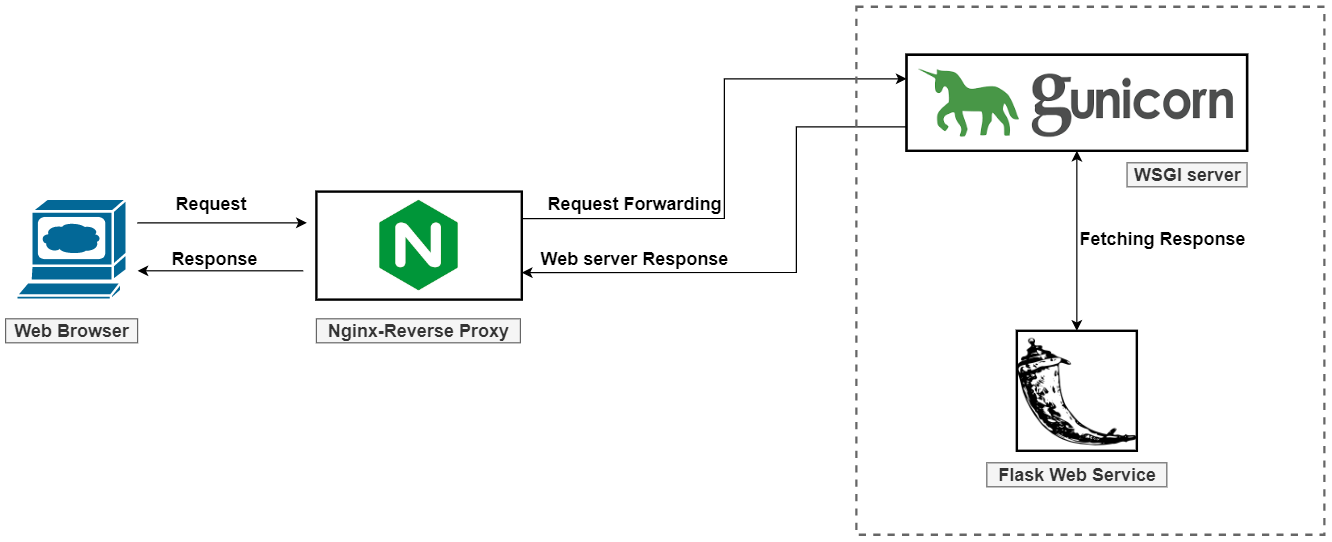
\includegraphics[scale=0.35]{figures/nginx_gunicorn_pythonapp.png}
	\caption{ Связка NGINX - gunicorn - Python-webapp}\label{fig:nginx_gunicron_pythonapp}
\end{figure}



\section{Приемы разработки web-приложений с помощью FastAPI}

Много полезных материалов можно найти на официальном сайте FastAPI \url{https://fastapi.tiangolo.com/}.

Установка необходимых компонентов
\begin{lstlisting}[
style = bash,
numbers = none	
]
pip install wheel -U
pip install uvicorn fastapi pydantic
\end{lstlisting}

\texttt{uvicorn} \url{https://www.uvicorn.org/} -- это ASGI веб-сервер\footnote{Не путать с \texttt{gunicorn} (\texttt{gunicorn} -- это WSGI-сервер, созданный для использования в UNIX-системах)}. 

Последнюю часть URL, начинающуюся с первого символа \verb|/|, называют endpoint или маршрутом (route). Например, в URL \texttt{https://example.com/items/foo} путем (конечной точкой или маршрутом) будет \texttt{/items/foo}.

Под операциями понимаются http-методы:
\begin{itemize}
	\item \texttt{POST}: создание данных,
	
	\item \texttt{GET}: чтение данных,
	
	\item \texttt{PUT}: обновление данных,
	
	\item \texttt{DELETE}: удаление данных,
	
	\item \texttt{OPTIONS},
	
	\item \texttt{HEAD},
	
	\item \texttt{PATCH},
	
	\item \texttt{TRACE}
\end{itemize}

Пример
\begin{lstlisting}[
style = ironpython,
title = {\sffamily main.py},
numbers = none
]
from fastapi import FastAPI

app = FastAPI()

@app.get("/") # HTTP-метод GET на пути /
async def root():
    return {"message" : "Hello World"}
\end{lstlisting}

Здесь \verb|@app.get("/")| говорит FastAPI, что задекорированная функция отвечает за обработку запросов, которые идут на <<корень>> web-сервиса, используя метод GET.

Функция \texttt{root} будет вызываться всякий раз, когда web-сервис получает запрос на <<корень>>, то есть на \verb|"/"| с использованием метода GET.

Аналогично можно использовать и другие операции: \verb|@app.post()|, \verb|@app.put()|, \verb|@app.delete()| и т.д.

Запустить приложение из командной строки можно так
\begin{lstlisting}[
style = bash,
numbers = none	
]
uvicorn main:app --reload # reload для перезапуска сервера после внесения изменений в код
\end{lstlisting}

Можно подставлять аргументы в маршрут. Например
\begin{lstlisting}[
style = ironpython,
numbers = none	
]
from fastapi import FastAPI

app = FastAPI()

# http://127.0.0.1:8000/items/foo -> item_id = "foo"
@app.get("/items/{item_id}")
async def read_item(item_id): # item\_id = "foo"
    return {"item_id" : item_id}
\end{lstlisting}

Теперь, если запустить этот пример как
\begin{lstlisting}[
style = bash,
numbers = none	
]
http://127.0.0.1:8000/items/foo
\end{lstlisting}
то значение \verb|"foo"| из маршрута будет передано функции \texttt{read\_item} в виде аргумента \texttt{item\_id}.

Можно явно указывать тип параметра в функции
\begin{lstlisting}[
style = ironpython,
numbers = none	
]
from fastapi import FastAPI

app = FastAPI()

@app.get("/items/{item_id}")
async def read_item(item_id: int):
     return {"item_id" : item_id}
\end{lstlisting}

FastAPI действительно проверяет тип параметров. И если тип параметра не соответствует указанному в функции, то возникает ошибка.

Если нужно передать какой-то путь, то следует использовать такой синтаксис \texttt{/files/{file\_path:path}}
\begin{lstlisting}[
style = ironpython,
numbers = none	
]
from fastapi import FastAPI

app = FastAPI()

# например, localhost:8000/files//leor.finkelberg/python -> file_path = "/leor.finkelberg/python"
@app.get("/files/{file_path:path}")
async def read_file(file_path: str):
    return {"file_path" : file_path}
\end{lstlisting}

Еще можно использовать значения параметров, передаваемые в запросе, но не имеющие отношения к пути. Такие параметры передаются парами после знака вопроса и отделяются друг от друга знаком амперсанда, то есть
\begin{lstlisting}[
style = bash,
numbers = none	
]
http://127.0.0.1:8000/10?key1=value1&key2=value2&...
\end{lstlisting}
\begin{lstlisting}[
style = ironpython,
numbers = none	
]
from fastapi import FastAPI

app = FastAPI()


# http://127.0.0.1:8000/items/10?solver_type=iterative
@app.get("/items_id/{item_id}")
async def read_item(item_id: int, solver_type: str = "direct"):
    return {"item_id" : item_id, "type" : solver_type} # {"item_id" : 10, "type" : "iterative"}
\end{lstlisting}

В запросе можно передавать булевы значения
\begin{lstlisting}[
style = bash,
numbers = none	
]
http://127.0.0.1:8000/items/100?q=test&short=True
# или так
http://127.0.0.1:8000/items/100?q=test&short=true
# или так
http://127.0.0.1:8000/items/100?q=test&short=1
# или так
http://127.0.0.1:8000/items/100?q=test&short=on
# или так
http://127.0.0.1:8000/items/100?q=test&short=yes
\end{lstlisting}

Маршрут может содержать несколько параметров, значения которых будут передаваться в функцию как аргументы
\begin{lstlisting}[
style = ironpython,
numbers = none	
]
from typing import Optional, NoReturn
from fastapi import FastAPI

app = FastAPI()

# http://127.0.0.1:8000/users/1632/items/admin?q=test&short=true
@app.get("/users/{user_id}/items/{item_id}")
async def read_item(
	user_id: int, 
	item_id: str, 
	q: Optional[str] = None, 
	short: bool = False
) -> NoReturn:
	item = {"user_id" : user_id, "item_id" : item_id}
	if q:
		item.update({"q" : q})
	if not short:
		item.update(
			{"description" : "This is an ..."}
		)

	return item
\end{lstlisting}

С помощью специального класса \texttt{Query} можно добавить, например, ограничение по длине строки на значение параметра
\begin{lstlisting}[
style = ironpython,
numbers = none	
]
from typing import Optional, Dict

from fastapi import FastAPI, Query

app = FastAPI()

@app.get("/items/")
async def read_items(
    q: Optional[str] = Query(None, max_length=50) # если длина строки превысит 50 символов, то возникнет ошибка
) -> Dict:
    results = {"items" [{"item_id" : "Foo"}, {"item_id" : "Bar"}]}
    if q:
        results.update({"q" : q})
    return results
\end{lstlisting}

ЗАМЕЧАНИЕ: конструкция \texttt{q: Optional[str] = Query(None)} эквивалентна конструкции \texttt{q: Optional[str] = None}, но первый вариант более явный. То есть с помощью \texttt{Query(None)} передается значение по умолчанию \texttt{None}, но без ограничений на строковую константу.

Разумеется можно добавить и ограничение на минимальную длину строки
\begin{lstlisting}[
style = ironpython,
numbers = none	
]
@app.get("/items/")
async def read_items(
    q: Optional[str] = Query(
        None,
        min_length=3,
        max_length=50
    )
) -> Dict:
    ...
\end{lstlisting}

Есть возможность добавить регулярное выражение
\begin{lstlisting}[
style = ironpython,
numbers = none	
]
@app.get("/items/")
async def read_items(
    q: Optional[str] = Query(
        None,
        min_length=3,
        max_length=50,
        regex="^.*python.*$"
    )
)
\end{lstlisting}

С помощью \texttt{Query} можно задавать значения по умолчанию и отличные от \texttt{None}
\begin{lstlisting}[
style = ironpython,
numbers = none
]
@app.get("/items/")
async def read_items(
    q: str = Query(
        "fixedquery",
        min_length=3
    )
) -> Dict:
    ...
\end{lstlisting}

Чтобы сделать параметр обязательным, нужно просто не передавать ему значение по умолчанию и не использовать класс \texttt{Query}. Однако, даже когда используется класс \texttt{Qeury} параметр можно сделать обязательным, передав ему в качестве значения по умолчанию многоточие (\texttt{...})
\begin{lstlisting}[
style = ironpython,
numbers = none	
]
@app.get("/items/")
async def read_items(
    q: str = Query(
        ..., # многоточие сообщает FastAPI, что параметр `q` обязательный
        min_length=3
    )
) -> Dict:
    ...
\end{lstlisting}

При таком способе определения параметра со значением по умолчанию сохраняются все преимущества использования ограничений, накладываемых на параметр.

Для того чтобы сообщить FastAPI, что параметр может встречаться в URL \emph{несколько} раз, можно использовать следующую конструкцию
\begin{lstlisting}[
style = ironpython,
numbers = none	
]
# http://localhost:8000/items/?q=test&q=fortran
@app.get("/items/")
async def read_items(
    q: Optional[List[str]] = Query(None) # <- NB: обязательно нужен класс Query
) -> Dict:
    query_items = {"q" : q}
    return query_items # {"q":["test","fortran"]}
\end{lstlisting}

Чтобы объявить параметр запроса с типом списка, как в примере выше, необходимо явно использовать класс \texttt{Query}. Иначе параметр запроса будет интерпретироваться как тело запроса.

Для параметра, который встречается в URL несколько раз, можно явно передать список его значений
\begin{lstlisting}[
style = ironpython,
numbers = none
]
# http://localhost:8000/items
@app.get("/items/")
async def read_items(
    q: List[str] = Query(
        ["foo", "bar"]
    )
) -> Dict:
    query_items = {"q" : q}
    return qeury_items
\end{lstlisting}

ЗАМЕЧАНИЕ: проверить работоспособность функции \texttt{read\_items} с методом \texttt{GET} (читать) можно несколькими способами:
\begin{itemize}
	\item набрав в поисковой строке браузера, например, \texttt{http://localhost:8000/items/88}; тогда в ответ в браузере появится что-нибудь вроде \verb|{"item" : 88}|,
	
	\item или с помощью утилиты \texttt{curl}
\begin{lstlisting}[
style = bash,
numbers = none	
]
curl -X 'GET' \
  'http://localhost:8000/items/88' \
  -H 'accept: application/json'
\end{lstlisting}
\end{itemize}

Если требуется в URL указать параметр, имя которого считается недопустимым с точки зрения Python, то можно воспользоваться специальным параметром \texttt{alias} класса \texttt{Query}
\begin{lstlisting}[
style = ironpython,
numbers = none	
]
# http://localhost:8000/items/?item-query=fortran
@app.get("/items/")
async def read_items(
    q: Optional[str] = Query(
        None,
        alias="item-query"
    ) # q <-> item-query
) -> Dict:
    results = {"items" : [{"item_id" : "Foo"}, {"item_id" : "Bar"}]}
    if q: 
        results.update({"q" : q})
    return results # {"items":[{"item_id":"Foo"},{"item_id":"Bar"}],"q":"fortran"}
\end{lstlisting}

Можно пометить параметр как <<устаревший>> с помощью параметра \texttt{depricated} класса \texttt{Query}.

Ванильный Python ругается, если первым в функции указать параметр со значением по умолчанию (ведь сначала должны идти позиционные аргументы, а уже потом аргументы со значением по умолчанию), но для FastAPI это не имеет никакого значения.

Как и в ванильном Python при объявлении функции можно использовать \verb|*|, для того чтобы сообщить FastAPI о том, что аргументам, стоящим справа от звездочки значения следует передавать явно (то есть по имени), а не позиционно
\begin{lstlisting}[
style = ironpython,
numbers = none	
]
from fastapi import FastAPI, Path

app = FastAPI()

@app.get("/items/{item_id}")
async def read_items(
    *, # для FastAPI порядок позиционных и именновых аргументов не имеет значения
    item_id: int = Path(
        ..., # значения по умолчанию у item_id нет (обязательный параметр)
        title="The ID of the item to get"
    ),
    q: str
) -> Dict:
    results = {"item_id": item_id}
    if q:
        results.update({"q": q})
    return results
\end{lstlisting}

ВАЖНО: класс \texttt{Path} работает также как и класс \texttt{Query}, но только для переменных в контексте маршрута, например, \verb|"/items/{item_id}"|. Класс \texttt{Query} применяется для аргументов, не относящихся к маршруту.

Ограничения можно накладывать разумеется не только на строковые константы, но и на вещественные значения аргументов функции
\begin{lstlisting}[
style = ironpython,
numbers = none
]
@app.get("/items/{item_id}")
async def read_items(
    *, # аргументам, расположенным правее *, значения следует передавать по имени
    item_id: int = Path(
        ..., # нет значения по умолчанию
        title="The ID ...",
       ge=1 # "Greate than or Equal", т.е. >= 1
    ),
    q: str,
) -> Dict:
    results = {"item_id" : item_id}
    if q:
        results.update({"q" : q})
    return results
\end{lstlisting}

Более сложный пример, обобщающий рассмотренные выше приемы оформления аргументов, относящихся и не относящихся к пути
\begin{lstlisting}[
style = ironpython,
numbers = none	
]
# http://localhost:8000/items/1632?num_of_cores=12
@app.get("/items/{item_id}")
async def read_items(
    item_id : int = Path(
        ... # у item_id нет значения по умолчанию (обязательный параметр)
    ), 
    *, # аргументам, стоящим справа от *, следует передавать значение по имени
    q: Optional[str] = Query( # необязательный параметр, принимающий объект опционального типа
        None,
        alias="item-query", # псевдоним
        title="Query string",
        desctiption="Query string for the items to search in the database that...",
        min_length=3,
        max_length=50,
        regex="^.*python.*$",
        deprecated=True,
    ),
    solver_type: str = Query(
        "direct" # значение по умолчанию для переменной, не имеющей отношение к пути
    ),
    num_of_cores: int = Query(
        10, # значение по умолчанию для переменной, не имеющей отношение к пути
        ge=8, # >= 8
        le=15, # <= 15
    )
) -> Dict:
    results = {"items" : item_id, "solver_type" : solver_type, "num_of_cores" : num_of_cores}
    if q:
        results.update({"q" : q})
    
    return results # {"items":1632,"solver_type":"direct","num_of_cores":12}
\end{lstlisting}

Аналогично можно задать ограничения и для вещественных значений: для вещественных значений следует указывать строгие условия (\texttt{>}, \texttt{<}, но не \texttt{<=} и т.д.)
\begin{lstlisting}[
style = ironpython,
numbers = none	
]
@app.get("/items/{item_id}")
async def read_items(
    *,
    item_id : int = Path(
        ..., # нет значения по умолчанию (обязательный параметр)
        ge=0, # >= 0
        le=1000, # <= 1000
    )
    q: str,
    size: float = Query(
        ..., # нет значения по умолчанию (обязательный параметр)
        gt=0, # > 0
        lt=10.5 # < 10.5
    )
)
\end{lstlisting}

Если нужно передать в запрос дополнительный параметр, не изменяя структуры сложных типов других параметров запроса, то можно воспользоваться классом \texttt{Body}
\begin{lstlisting}[
style = ironpython,
numbers = none	
]
from typing import Optional
from fastapi import Body, FastAPI
from pydantic import BaseModel

app = FastAPI()

class Item(BaseModel):
    name: str
    description: Optional[str] = None
    price: float
    tax: Optional[float] = None

class User(BaseModel):
    username: str
    full_name: Optional[str] = None

@app.put("/items/{item_id}")
async def update_item(
    item_id: int,
    item: Item,
    user: User,
    importance: int = Body(...)
):
    results = {
    	"item_id" : item_id, "item" : item,
    	"user" : user, "importance" : importance
    }
    return results
\end{lstlisting}

В этом случае FastAPI ожидает получить тело вида
\begin{lstlisting}[
style = bash,
numbers = none	
]
{
  "item" : {
    "name" : "Foo",
    "description" : "The pretender",
    "price" : 42.0,
    "tax" : 3.2 
  },
  "user" : {
    "username" : "dave",
    "full_name" : "Dave Grohl"
  },
  "importance" : 5
}
\end{lstlisting}

Кончено, вместе с \texttt{Body} можно передавать и обычные параметры запроса
\begin{lstlisting}[
style = ironpython,
numbers = none	
]
@app.put("/items/{item_id}")
async def update_item(
    *,
    item_id: int,
    item: Item,
    user: User,
    importance: int = Body(..., gt=0),
    q: Optional[str] = None
):
    ...
\end{lstlisting}

Если тело запроса должно быть вложенным, то это легко организовать с помощью параметра \texttt{embed}
\begin{lstlisting}[
style = ironpython,
numbers = none	
]
@app.put("/items/{item_id}")
async def update_item(
    item_id: int,
    item: Item = Body(..., embed=True)
) -> Dict:
    results = {"item_id" : item_id, "item" : item}
    return results
\end{lstlisting}

В этом случае FastAPI будет ожидать тело вида
\begin{lstlisting}[
style = bash,
numbers = none	
]
{
  "item" : {
    "name" : "Foo",
    "description" : "The pretender",
    "price" : 42.0,
    "tax" : 3.2
  }
}
\end{lstlisting}
вместо
\begin{lstlisting}[
style = bash,
numbers = none	
]
{
  "name" : "Foo",
  "description" : "The pretender",
  "price" : 42.0,
  "tax" : 3.2
}
\end{lstlisting}

Так же как и для классов \texttt{Query}, \texttt{Path} и \texttt{Body} можно организовать дополнительную проверку внутри классов \texttt{pydantic} с помощью \texttt{Field}
\begin{lstlisting}[
style = ironpython,
numbers = none	
]
from typing import Optional

from fastapi import Body, FastAPI
from pydantic import BaseModel, Field

app = FastAPI()

class Item(BaseModel):
    name: str
    desctiption: Optional[str] = Field(
        None,
        title = "The desc...",
        max_length=300
    )
    price: float = Field(
        ..., # нет значения по умолчанию
        gt=0,
        description="The ...",
    )
    tax: Optional[float] = None
    
@app.put("/items/{item_id}")
async def update_item(
    item_id: int,
    item: Item = Body(
        ...,
        embed=True
    )
) -> Dict:
    results = {"item_id" : item_id, "item" : item}
    return results
\end{lstlisting}

\texttt{Field} работает так же как \texttt{Query}, \texttt{Path} и \texttt{Body} и принимает те же параметры.

Можно объявить тип возвращаемого объекта в параметре \texttt{response\_model}
\begin{lstlisting}[
style = ironpython,
numbers = none	
]
# НИ В КОЕМ СЛУЧАЕ НЕ ДЕЛАТЬ ТАК В ПРОДЕ!!!
class UserIn(BaseModel):
    username: str
    password: str
    email: EmailStr
    full_name: Optional[str] = None

# создать пользователя с помощью метода POST
@app.post("/user/", response_model=UserIn)
async def create_user(user: UserIn):
    return user
\end{lstlisting}

Здесь класс \texttt{UserIn} используется как для объявления входных данных, так и выходных данных. Теперь, когда создается пользователь с паролем, этот пароль возвращается в ответе.

Проверить работу функции \texttt{create\_user} с методом \texttt{POST} можно так
\begin{lstlisting}[
style = bash,
numbers = none	
]
curl -X 'POST' \
  'http://localhost:8000/user/' \
  -H 'accept: application/json' \
  -H 'Content-Type: application/json' \
  -d '{
    "username": "string",
    "password": "string",
    "email": "user@example.com",
    "full_name": "string"
}'
\end{lstlisting}

Можно создать класс для описания выходной модели без поля для пароля
\begin{lstlisting}[
style = ironpython,
numbers = none	
]
class UserIn(BaseModel):
    username: str
    password: str
    email: EmailStr
    full_name: Optional[str] = None

class UserOut(BaseModel):
    username: str
    email: EmailStr
    full_name: Optional[str] = None


@app.post("/user/", response_model=UserOut)
async def create_user(user: UserIn):
    return user
\end{lstlisting}

ЗАМЕЧАНИЕ: в функциях с методом \texttt{POST} (создать), как в пример выше
\begin{lstlisting}[
style = ironpython,
numbers = none	
]
@app.post("/items/", response_model=UserOut) # POST
async def create_user(user: UserIn):
    return user
\end{lstlisting}
соответствующий аргумент функции (в данном случае аргумент \texttt{user}) связывается с json-объектом, который передается через флаг \verb|-d| в \texttt{curl}. То есть неявно переменная \texttt{user} как бы получает ссылку на json-объект. В функциях с методом \texttt{GET} (читать) значение переменной функции передается в маршруте, например
\begin{lstlisting}[
style = ironpython,
numbers = none	
]
@app.get("/items/{item_id}")
async def read_items(item_id: int):
    ...
\end{lstlisting}

Для проверки работы функции с новой классом на выходных параметров воспользуемся таким запросом
\begin{lstlisting}[
style = bash,
numbers = none	
]
curl -X 'POST' \
  'http://localhost:8000/user/' \
  -H 'accept: application/json' \
  -H 'Content-Type: application/json' \
  # то, что передается через -d связывается с аргументом user функции create_user, объявленной выше
  -d '{ 
    "username": "Leor",
    "password": "Evdimonia",
    "email": "leor.finkelberg@yandex.ru",
    "full_name": "Leor Finkelberg"
}'
\end{lstlisting}

Но ответ не будет содержать пароля
\begin{lstlisting}[
style = bash,
numbers = none	
]
{ # без пароля!
  "username": "Leor",
  "email": "leor.finkelberg@yandex.ru",
  "full_name": "Leor Finkelberg"
}
\end{lstlisting}

Если ответы содержат много параметров со значением по умолчанию, а интерес представляют только те параметры, которым были переданы значения явно в текущей сессии, то можно использовать параметр \texttt{response\_model\_exclude\_unset}
\begin{lstlisting}[
style = ironpython,
numbers = none
]
@app.get(
    "/items/{item_id}",
    response_model=Item,
    response_model_exclude_unset=True # <- NB
)
async def read_item(item_id: str):
    ...	
\end{lstlisting}

Тогда ответ будет содержать только те параметры, которым были переданны значения в текущей сессии (параметры со значениями по умолчанию будут опущены).

Отфильтровать параметры на выходе можно с помощью параметров \texttt{response\_model\_exclude} и \texttt{response\_model\_exclude}
\begin{lstlisting}[
style = ironpython,
numbers = none	
]
@app.get(
    "/items/{item_id}/name",
    response_model=Item,
    response_model_include={"name", "description"},
)
async def read_item_name(item_id: str):
    return items[item_id] # ответ будет включать только ключи name и description

@app.get(
    "/items/{item_id}/public",
    response_model=Item,
    response_model_exclude={"tax"}
)
async def read_item_public_data(item_id: str):
    return items[item_id] # ответ будет включать все ключи кроме tax
\end{lstlisting}

Обновлять данные можно с помощью метода \texttt{PUT}
\begin{lstlisting}[
style = ironpython,
numbers = none	
]
from typing import List, Optional

from fastapi import FastAPI
from fastapi.encoders import jsonable_encoder
from pydantic import BaseModel

app = FastAPI()


class Item(BaseModel):
    name: Optional[str] = None
    description: Optional[str] = None
    price: Optional[float] = None
    tax: float = 10.5
    tags: List[str] = []


items = {
	"foo": {"name": "Foo", "price": 50.2},
	"bar": {"name": "Bar", "description": "The bartenders", "price": 62, "tax": 20.2},
	"baz": {"name": "Baz", "description": None, "price": 50.2, "tax": 10.5, "tags": []},
}


@app.get("/items/{item_id}", response_model=Item) # GET
async def read_item(item_id: str):
    return items[item_id]


@app.put("/items/{item_id}", response_model=Item) # PUT
async def update_item(item_id: str, item: Item):
    update_item_encoded = jsonable_encoder(item)
    items[item_id] = update_item_encoded
    return update_item_encoded
\end{lstlisting}

Теперь чтобы обновить данные направим два запроса
\begin{lstlisting}[
style = bash,
numbers = none
]
$ curl -X 'PUT' \
  'http://localhost:8000/items/2' \
  -H 'accept: application/json' \
  -H 'Content-Type: application/json' \
  -d '{
    "name": "Ansys",
    "description": "CAE package...",
    "price": 250,
    "tax": 0.5,
    "tags": []
}'
$ curl -X 'PUT' \
  'http://localhost:8000/items/42' \
  -H 'accept: application/json' \
  -H 'Content-Type: application/json' \
  -d '{
    "name": "Nastran",
    "description": "CAE package...",
    "price": 480,
    "tax": 8.5,
    "tags": []
}'
\end{lstlisting}

А чтобы прочитать данные запросы для разных идентификационных номеров должны выглядеть так
\begin{lstlisting}[
style = bash,
numbers = none
]
$ curl -X 'GET' \
  'http://localhost:8000/items/2' \
  -H 'accept: application/json' # вернет json для Ansys
$ curl -X 'GET' \
  'http://localhost:8000/items/42' \
  -H 'accept: application/json' # вернет json для Nastran
\end{lstlisting}

В случае, когда данные требуется обновлять частично, удобно использовать \texttt{exclude\_unset}
\begin{lstlisting}[
style = ironpython,
numbers = none	
]
class Item(BaseModel):
	name: Optional[str] = None
	description: Optional[str] = None
	price: Optional[float] = None
	tax: float = 10.5
	tags: List[str] = []

@app.patch("/items/{item_id}", response_model=Item) # PATCH
	async def update_item(item_id: str, item: Item):
	stored_item_data = items[item_id]
	stored_item_model = Item(**stored_item_data)
	update_data = item.dict(exclude_unset=True) # <- NB
	updated_item = stored_item_model.copy(update=update_data)
	items[item_id] = jsonable_encoder(updated_item)
	return updated_item
\end{lstlisting}

Теперь будут учитываться только те значения, которые были переданы явно (т.е. значения по умолчанию учитываться не будут).

Еще можно создавать так называемые подприложения. Пример
\begin{lstlisting}[
style = ironpython,
numbers = none	
]
from fastapi import FastAPI

app = FastAPI()

@app.get("/app")
async def read_main():
    return {"message" : "Hello World from main app"}
    
subapi = FastAPI()

@subapi.get("/sub")
async def read_sub():
    return {"message" : "Hello World from sub API"}
\end{lstlisting}

Вызов может выглядеть так
\begin{lstlisting}[
style = bash,
numbers = none	
]
http://localhost:8000/app # {"message":"Hello world from main app"}
http://localhost:8000/subapi/sub # {"message":"Hello world from sub API"}
\end{lstlisting}

Для упрощения процедуры передачи данных в приложение, удобно использовать web-сокеты. Пример
\begin{lstlisting}[
title = {\sffamily main.py},
style = ironpython,
numbers = none	
]
from fastapi import FastAPI, WebSocket
from fastapi.responses import HTMLResponse

app = FastAPI()

html = """
<!DOCTYPE html>
<html>
  <head>
    <title>Main form for ML-app</title>
  </head>
  <body>
    <h1>Enter your params here</h1>
    <form action="" onsubmit="sendMessage(event)">
      <input type="text" id="messageText" autocomplete="off"/>
      <button>Run</button>
    </form>
    <ul id='messages'>
    </ul>
    <script>
      var ws = new WebSocket("ws://localhost:8000/ws");
      ws.onmessage = function(event) {
	    var messages = document.getElementById('messages')
	    var message = document.createElement('li')
	    var content = document.createTextNode(event.data)
	    message.appendChild(content)
	    messages.appendChild(message)
      };
      function sendMessage(event) {
	    var input = document.getElementById("messageText")
	    ws.send(input.value)
	    input.value = ''
	    event.preventDefault()
      }
    </script>
  </body>
</html>
"""

@app.get("/")
async def get():
    return HTMLResponse(html)


@app.websocket("/ws")
async def websocket_endpoint(websocket: WebSocket):
    await websocket.accept()

    while True:
        data = await websocket.receive_text()
        await websocket.send_text(f"Message text was: {data}")
\end{lstlisting}

Запускаем как обычно
\begin{lstlisting}[
style = ironpython,
numbers = none	
]
uvicorn main:app --reload
\end{lstlisting}
Если все прошло как полагается, то по маршруту \texttt{http://localhost:8000} должна быть доступна форма-интерфейс.

Если требуется, чтобы какие-то операции были выполнены перед запуском приложения, то это можно следующим образом
\begin{lstlisting}[
style = ironpython,
numbers = none	
]
from fastapi import FastAPI

app = FastAPI()

items = {}

@app.on_event("startup")
async def startup_event():
    items["foo"] = {"name" : "Fighters"}
    items["bar"] = {"name" : "Tenders"}
    
@app.get("/items/{item_id}")
async def read_items(item_id: str):
    return items[item_id]
\end{lstlisting}

То есть в данном случае, перед запуском приложения будет создан словарь \texttt{items}.

Аналогично можно создать функцию, которая будет вызываться по завершении работы приложения
\begin{lstlisting}[
style = ironpython,
numbers = none	
]
from fastapi import FastAPI

app = FastAPI()

@app.on_event("shutdown")
def shutdown_event():
    with open("log.txt", "a") as log:
        log.write("Application shutdown")
        
@app.get("/items/")
async def read_items():
    return [{"name" : "Foo"}]
\end{lstlisting}

Иногда бывает нужно использовать в сессии пользовательские переменные окружения. Сделать это можно так
\begin{lstlisting}[
style = ironpython,
numbers = none
]
# ADMIN_EMAIL="leor.finkelberg@yandex.ru" APP_NAME="CAD.ai" uvicorn main:app
from fastapi import FastAPI
from pydantic import BaseSettings

class Settings(BaseSettings):
    app_name: str = "Awesome API"
    admin_email: str
    items_per_user: int = 50

settings = Settings()
app = FastAPI()

@app.get("/info")
async def info():
    return {	
    	"app_name": settings.app_name,
    	"admin_email": settings.admin_email,
    	"items_per_user": settings.items_per_user,
    } # {"app_name":"CAD.ai","admin_email":"leor.finkelberg@yandex.ru","items_per_user":50}
\end{lstlisting}

Тогда запуск приложения будет выглядеть следующим образом
\begin{lstlisting}[
style = ironpython,
numbers = none	
]
ADMIN_EMAIL="leor.finkelberg@yandex.ru" APP_NAME="CAD.ai" uvicorn main:app
\end{lstlisting} 

Вот еще один любопытный способ использовать информацию, представленную в конфигурационном файле. Этот способ может быть полезен в ситуациях, когда только часть параметров изменяется в зависимости от окружения.

Создадим скрытый файл \texttt{.env}
\begin{lstlisting}[
title = {\sffamily .env},
style = bash,
numbers = none	
]
# здесь используются только те параметры, котрые изменяются в зависимости от окружения
ADMIN_EMAIL="leor.finkelberg@yandex.ru"
APP_NAME="CAD.ai"
\end{lstlisting}

Затем создадим модуль, который будет вычитывать конфигурацию
\begin{lstlisting}[
title = {\sffamily config.py},
style = ironpython,
numbers = none	
]
from pydantic import BaseSettings

class Settings(BaseSettings):
    # это базовые параметры
    app_name: str = "Awesome API"
    admin_email: str
    items_per_user: int = 50

    class Config:
        env_file = ".env" # здесь используются только те параметры, котрые изменяются в зависимости от окружения
\end{lstlisting}

А затем собственно модуль, который будет использовать данные из конфигурационного файла
\begin{lstlisting}[
title = {\sffamily main.py},
style = ironpython,
numbers = none
]
from functools import lru_cache
from fastapi import Depends, FastAPI
from config import Settings

app = FastAPI()

@lru_cache()
def get_settings():
    return Settings()

@app.get("/info")
async def info(settings: Settings = Depends(get_settings)):
    return {
	    "app_name" : settings.app_name,
	    "admin_email" : settings.admin_email,
	    "items_per_user" : settings.items_per_user,
    } # {"app_name":"CAD.ai","admin_email":"leor.finkelberg@yandex.ru","items_per_user":50}
\end{lstlisting}

\subsection{Развертывание FastAPI-приложений на платформе Deta}

Структура проекта для развертывания на платформе Deta \url{https://www.deta.sh/?ref=fastapi}
\begin{lstlisting}[
style = bash,
numbers = none	
]
.
 `-- main.py
 `-- requirements.txt
\end{lstlisting}

Модуль \texttt{main.py} имеет следующее содержание
\begin{lstlisting}[
title = {\sffamily main.py},
style = ironpython,
numbers = none	
]
from fastapi import FastAPI

app = FastAPI()

@app.get("/")
def read_root():
    return {"Hello": "World"}

@app.get("/items/{item_id}")
def read_item(item_id: int):
    return {"item_id": item_id}
\end{lstlisting}
а файл с зависимостями такое содержание
\begin{lstlisting}[
style = bash,
numbers = none	
]
fastapi
\end{lstlisting}

Устанавливать \texttt{uvicorn} для развертывания на Deta не нужно!!!

Теперь нужно создать бесплатный аккаунт на Deta. Устанавливаем утилиту командной строки \texttt{deta}
\begin{lstlisting}[
style = bash,
numbers = none	
]
curl -fsSL https://get.deta.dev/cli.sh | sh
\end{lstlisting}

После чего нужно залогиниться
\begin{lstlisting}[
style = bash,
numbers = none	
]
deta login
\end{lstlisting}
и, находясь в корне проекта, запустить процедуру развертывания
\begin{lstlisting}[
style = bash,
numbers = none
]
deta new
----------------
{
	"name": "fastapideta",
	"runtime": "python3.7",
	"endpoint": "https://qltnci.deta.dev", # <---- NB
	"visor": "enabled",
	"http_auth": "enabled"
}
\end{lstlisting}

Для того чтобы убедиться в работоспособности приложения нужно вставить в браузер URL, созданный платформой Deta (в данном случае это \texttt{https://qltnci.deta.dev}).

Чтобы можно было делиться этой ссылкой следует выполнить <<публичную аунтификацию>>
\begin{lstlisting}[
style = bash,
numbers = none	
]
deta auth disable
\end{lstlisting}


\subsection{Развертывание FastAPI-приложения в ручную}

Для того чтобы развернуть FastAPI-приложение в ручную нужно просто установить ASGI-совместимый сервер
\begin{lstlisting}[
style = bash,
numbers = none	
]
pip install uvicorn[standard]
\end{lstlisting}

И запустить приложение, как обычно, но без опции \verb|--reload|
\begin{lstlisting}[
style = bash,
numbers = none
]
uvicorn main:app --host 0.0.0.0 --port 80
\end{lstlisting}


\section{Приемы разработки приложений с графическим интерфейсом пользователя с использованием библиотеки DearPyGui}


\section{Использование Google Drive как хранилище артифактов ML-пайплайнов}

Чтобы работать с файлом, размещенным на Google Drive, нужно просто выбрать интересующий файл, открыть публичный доступ к нему \directory{Открыть доступ > Разрешить доступ всем, у кого есть ссылка} и скопировать ссылку
\begin{lstlisting}[
style = ironpython,
numbers = none	
]
import pandas as pd
import requests

url = "https://drive.google.com/file/d/1-7TLGI-6zHxM3ASkCQj6yMLg6mEu5q9n/view?usp=sharing"
download_path = 5"https://drive.google.com/uc?export=download&id={}".format(url.split('/')[-2])
# 'https://drive.google.com/uc?export=download&id=1-7TLGI-6zHxM3ASkCQj6yMLg6mEu5q9n'

df = pd.read_csv(download_path)
df.head()
\end{lstlisting}


\section{Конфигурационные файлы как интерфейс доступа к Python-сценарию}

Конфигурационный файл может использоваться как интерфейс доступа к Python-приложению. Пример файла конфигурации
\begin{lstlisting}[
	style = bash,
	title = {\sffamily config.yaml},
	numbers = none	
	]
	input_data_path: "ml_example/data/raw/train.csv" # относительно корня проекта
	output_model_path: "models/model.pkl"
	metric_path: "models/metrics.json"
	splitting_params:
	val_size: 0.1
	random_state: 3
	train_params:
	model_type: "RandomForestRegressor"
	feature_params: # этому элементу соответствует класс FeatureParams
	  categorical_features:
  	    - "MSZoning"
	    - "Neighborhood"
	    - "RoofStyle"
	    ...
\end{lstlisting}

Чтобы использовать значения из конфигурационного файла в приложении, следует прочитать этот файл с помощью библиотеки \texttt{yaml}
\begin{lstlisting}[
style = ironpython,
numbers = none	
]
import yaml
	
with open("config.yaml", "r") as f:
	config = yaml.safe_load(f) # config -- это обычный словарь
\end{lstlisting}

Однако в данном случае не проверяются типы переданных значений. Для организации проверки типов можно использовать модуль \texttt{dataclasses}
\begin{lstlisting}[
style = ironpython,
title = {\sffamily train\_pipeline\_params.py},
emph = {read_training_pipeline_params},
numbers = none	
]
from dataclasses import dataclass
from .split_params import SplittingParams
from .feature_params import FeatureParams
from .train_params import TrainingParams
from marshmallow_dataclass import class_schema
import yaml

@dataclass()
class TrainingPipelineParams:
    """
    Главный класс для построения схемы конфигурационного файла
    """
    input_data_path: str
    output_model_path: str
    metric_path: str
    splitting_params: SplittingParams
    feature_params: FeatureParams
    train_params: TrainingParams

TrainingPipelineParamsSchema = class_schema(TrainingPipelineParams)

def read_training_pipeline_params(path: str) -> TrainingPipelineParams:
    with open(path, "r") as input_stream:
        schema = TrainingPipelineParamsSchema()
    return schema.load(yaml.safe_load(input_stream)) # возвращает объект, к полям которого можно обращаться с помощью точечной нотации
\end{lstlisting}

Пример класса для построения схемы подэлемента конфигурационного файла
\begin{lstlisting}[
title = {\sffamily feature\_params.py},
style = ironpython,
numbers = none
]
from dataclasses import dataclass, field
from typing import List, Optional

@dataclass()
class FeatureParams:
    """
    Класс для построения схемы подэлемента конфигурационного файла.
    Соответствует элементу feature_params файла config.yaml
    """
    categorical_features: List[str]
    numerical_features: List[str]
    features_to_drop: List[str]
    target_col: Optional[str]
    use_log_trick: bool = field(default=True) # <- 
\end{lstlisting}

Например, если
\begin{lstlisting}[
style = ironpython,
numbers = none	
]
params = read_training_pipeline_params("config.yaml")
\end{lstlisting}
то вызвать значение, скажем, \texttt{use\_log\_trick} можно так
\begin{lstlisting}[
style = ironpython,
numbers = none	
]
params.feature_params.use_log_trick # вернет True (так как это значение по умолчанию в классе FeatureParams)
\end{lstlisting}


\section{Упаковка ML-пайплайна в docker-образ}

В целом порядок работы выглядит следующим образом:

\begin{itemize}
	\item пишем ML-пайплайн, который, скажем, обучает модель случайного леса для задачи регрессии,
	
	\item тестируем этот ML-пайплайн, смотрим на метрики и пр.,
	
	\item когда нам кажется, что пайплайн работает как полагается,
	\begin{itemize}
		\item либо сохраняем обученную модель (модель обучается не в контейнере!) в формате \texttt{.pkl} в облачном хранилище (например, в S3),
		
		\item либо (если по каким-то соображением требуется, чтобы модель обучалась в контейнере) собираем проект с ML-пайплайном в пакет с помощью \texttt{python setup.py sdist bdist\_wheel} и публикуем его на PyPI с помощью \texttt{twine upload dist/*} (в директории \texttt{dist} будет лежать и tar-архив, и whl-архив); затем этот пакет можно будет установить с помощью утилиты \texttt{pip} внутри docker-образа; к слову, также можно собрать этот пайплайн и без публикации на PyPI: т.е. можно собрать ML-пайплайн в пакет с помощью \texttt{python setup.py sdist}, а затем установить пакет инструкцией \texttt{pip install dist/package\_name.tar.gz} внутри контейнера (но так лучше не делать!!!),

	    \item с помощью инструкции \texttt{pip install package\_name} или в более простом, но менее правильном случае, с помощью инструкции \texttt{pip install dist/package\_name.tar.gz} устанавливаем наш пакет в окружение docker-образа,
    
	    \item получаем доступ к пакету: получить доступ к нашему пакету можно следующим образом
	\end{itemize}
    \begin{itemize}
    	\item в файле \texttt{setup.py}, который используется при сборке пакета можно создать точку входа со специальным ключевым словом \texttt{console\_scripts}
\begin{lstlisting}[
title = {\sffamily setup.py},
style = ironpython,
]
from setuptools import find_packages, setup

setup(
    name="ml_example",
    packages=find_packages(),
    version="0.1.0",
    description="Example of ml project",
    author="Your name (or your organization/company/team)",
    entry_points={
        "console_scripts": [ # <-- NB
            "ml_example_train = ml_example.train_pipeline:train_pipeline_command"
            # в Dockerfile должны быть строки
            #     ENTRYPOINT ["ml_example_train]
            #     CMD ["confis/train_config.yaml"]
         ]
    },
    install_requires=[
        "click",
        "Sphinx",
        ...
        "marshmallow-dataclass==8.3.0",
        "pandas",
    ],
    license="MIT",
)
\end{lstlisting}
    Конструкцию на строке 11 (с оговорками) допустимо интерпретировать так: при запуске docker-контейнера (на базе образа Python), у которого в \texttt{Dockerfile} должна быть прописана инструкция \texttt{ENTRYPOINT} вида \texttt{ENTRYPOINT ["ml\_exmaple\_train"]} и инструкция \texttt{CMD ["configs/train\_config.yaml"]}, содержащая аргументы для \texttt{ENTRYPOINT}, объект \texttt{ml\_example\_train} будет преобразован в утилиту, которая строку
    
    \texttt{ml\_example.train\_pipeline:train\_pipeline\_command} превратит в
    
    \texttt{from ml\_example.train\_pipeline import train\_pipeline\_command} и запустит функцию \texttt{train\_pipeline\_command}, передав ей аргументы из \texttt{CMD}. В данном случае передача аргументов в функцию таким образом возможна, так как предполагается, что функция организована так
\begin{lstlisting}[
title = {\sffamily train\_pipeline.py},
emph = {train_pipeline_command},
style = ironpython,
numbers = none	
]
...
@click.command(name="train_pipeline")
@click.argument("config_path") # <- принимает значение, переданное как аргумент командной строки или переданное через инструкцию CMD файла Dockerfile
def train_pipeline_command(config_path: str):
    params = read_training_pipeline_params(config_path)
    train_pipeline(params)
...
\end{lstlisting}

    А сам \texttt{Dockerfile} может выглядеть так
\begin{lstlisting}[
style = bash,
numbers = none	
]
FROM python:3.6 # <-- NB
RUN mkdir -p /build
...
ENTRYPOINT ["ml_example_train"]
CMD ["configs/train_config.yaml"]
\end{lstlisting}
    \end{itemize}

    \item Подгружаем данные в docker-образ, например, из облачного хранилища,
    
    \item запускаем python-сценарий, который читает все, что нужно для его работы -- предобученную модель, данные, конфигурационные файлы и пр. -- ждем запроса от пользователя и возвращаем прогноз. 
\end{itemize}

ВАЖНО: на этапе проверки работы приложения стартовый сценарий, должен располагаться в корне проекта и использовать абсолютные пути (от корня проекта) до интересующих модулей и пакетов. При сборке пакета для публикации на PyPI РЕ нужно изменять пути (они как раньше должны включать все узлы цепочки импорта от корня проекта). Например, если директория, на основании которой мы собираемся сделать пакет для публикации на PyPI, называется \texttt{ml\_example} и лежит в корне проекта, то лежащие внутри нее модули, естественно, должны включать ее имя, например, \texttt{from ml\_example.data import read\_data}. После сборки проекта в пакет эти абсолютные пути по-прежнему будут иметь смысл, так как в этот поиск нужных модулей будет идти относительно имени опубликованного пакета.


\section{Приемы работы с \texttt{dataclass}}

Для того чтобы превратить обычный python-класс в дата-класс, который служит в числе прочего для валидации схемы конфигурационного файла\footnote{Или, проще говоря, для проверки типов значений, указанных в конфигурационном файле}, используемого в качестве интерфейса к python-приложению, нужно просто задекорировать соответствующий класс декоратором \texttt{dataclass}
\begin{lstlisting}[
title = {\sffamily ml\_example/entities/train\_pipelines\_params.py},
style = ironpython,
numbers = none	
]
import yaml
from dataclasses import dataclass, field
from marshmellow_dataclass import class_schema

# это модули, в которых содержится описание классов, которые
# будут использоваться как подтипы в главном дата-классе
from .feature_params import FeatureParams
from .split_params import SplittingParams
...

@dataclass()
class TrainingPipelineParams:
    # ожидается, что параметры с приведенными ниже именемами,
    # встретятся в конфигурационном файле
    input_data_path: str 
    output_model_path: str
    mertic_path: str
    feature_params: FeatureParams    # класс из ml_example/entities/feature_params.py
    spitting_params: SplittingParams # класс из ml_example/entities/split_params.py
    ...
    
TrainingPipelineParamsSchema = class_schema(TrainingPipelineParams)

def read_training_pipeline_params(
    path: str
) -> TrainingPipelineParams: # класс как тип
    with open(path, "r") as input_schema: # input_schema -- файловый объект
        schema = TrainingPipelineParamsSchema()
        return schema.load(yaml.safe_load(input_schema))
\end{lstlisting}

Типичный класс, который используется как подтип в главном дата-классе, имеет следующий вид
\begin{lstlisting}[
title = {\sffamily ml\_example/entities/feature\_params.py},
style = ironpython,
numbers = none	
]
from dataclasses import dataclass, field
from typing import List, Optional

@dataclass()
class FeatureParams:
    categorical_features: List[str],
    numerical_features: List[str],
    features_to_drop: List[str],
    target_col: Optional[str],
    use_log_trick: bool = field(default = True) # этого параметры нет в конфигурационном файле, но ни что не мешает его объявить в дата-классе
\end{lstlisting}

Этот подкласс отвечает следующему фрагменту кофигурационного файла
\begin{lstlisting}[
title = {\sffamily train\_config.yaml},
style = bash,
numbers = none	
]
...
feature_params:
  categorical_features:
    - "MSZoning"
    - "Neighborhood"
    ...
  numerical_features:
    - "OverallQual"
    - "MSSubClass"
    ...
  features_to_drop:
    - "YrSold"
  target_col: "SalePrice"
\end{lstlisting}



\section{Тестирование в Python}

Хранить тесты нужно в поддиректории \texttt{tests} пакета, приложения или библиотеки, к которым они относятся. Использование иерархии в дереве теста, которая повторяет иерархию модуля, сделает тесты более управляемыми. Это значит, что тест для кода \texttt{mylib/foobar.py} необходимо размещать в \texttt{mylib/tests/test\_foobar.py}. 

Имена тестов должны совпадать с именами тестируемых модулей, но с добавлением префикса или постфикса \texttt{test}, т.е. \texttt{test\_modulename} или \texttt{modulename\_test}. Это поможет \texttt{pytest} находить тесты.

\texttt{pytest} запущенный без аргументов или с указанием каталога ищет функции для тестирования рекурсивно в подкаталогах в соответствии с соглашением по именам:
\begin{itemize}
	\item файлы называются \texttt{test\_().py} или \texttt{()\_test.py},
	
	\item тестовые функции называются \texttt{test\_()},
	
	\item тестовые классы \texttt{Test()}.
\end{itemize}

Тесты бывают:
\begin{itemize}
	\item позитивные: пишутся просто через проверку \texttt{assert condition},
	
	\item негативные: пишутся через \texttt{with pytest.raises(TypeError)}; чтобы убедиться, что Python возбудил правильное исключение,
	
	\item граничные (подходит Hypothises).
\end{itemize}

Для оценки полноты покрытия кода тестами можно использовать плагин \texttt{pytest-cov} (показывает какие строки не исполнялись во время тестирования).

Для маленьких проектов с простым применением -- пакет \texttt{pytest}. Пакет \texttt{pytest} предоставляет команду \texttt{pytest}, которая загружает каждый файл, имя которого начинается на \texttt{test\_}, и затем выполняет все функции внутри каждого файла, если они тоже начинаются на \texttt{test\_}.

Запустить тест можно так
\begin{lstlisting}[
style = bash,
numbers = none	
]
pytest -v test_true.py
\end{lstlisting}

Флаг \verb|-v| выводит имя каждого теста в отдельной строке. Если тест не пройден, вывод меняется и отображается информация об ошибке.

Тест не проходит, как только возникает исключение \texttt{AssertationError}.

\subsection{Что можно тестировать в задачах анализа данных}

{\color{red} Концепция \emph{разработки через тестирование} (TDD) не работает в задачах машинного обучения и анализа данных.}

Что тестировать:
\begin{itemize}
	\item Функциональные тесты: результат, а не реализация
	
	\item Нефункциональные тесты: быстродействие
	
	\item Тесты производительности модели: если какой-то признак может поламать модель, тесты должны это показать
	
	\item Тесты собственно данных: имена колонок, границы, дубли и пр.
\end{itemize}



\subsection{Пример организации директории под тесты}

Если в директории, которая позиционируется как пакет, есть модуль \texttt{\_\_init\_\_.py}, то при импорте пакета (\texttt{import package}, \texttt{from my\_cool\_lib import package}) будет выполнено все, что написано в модуле  \texttt{\_\_init\_\_.py}. И если модуль \texttt{\_\_init\_\_.py}, например, импортирует какие-то функции из другого модуля, то эти функции станут частью пространства имен пакета, ассоциированного с модулем \texttt{\_\_init\_\_.py}.

Пример директории проекта
\begin{lstlisting}[
style = bash,
numbers = none	
]
myproject/
  -- main_part/
    -- __init__.py # from .simple_module import my_summa\n\n__all__ = ["my_summa"]
    -- simple_module.py # функция my_summa
  -- tests/
    -- __init__.py # пустой файл
    -- test_summa.py # from main_part import my_summa
\end{lstlisting}

\begin{lstlisting}[
title = {\sffamily main\_part/\_\_init\_\_.py},
style = ironpython,
numbers = none	
]
from .simple_module import my_summa # <- NB: относительный импорт модуля!!!

__all__ = ["my_summa"] # my_summa станет частью пространства имен пакета main_part
\end{lstlisting}

\begin{lstlisting}[
title = {\sffamily simple\_module.py},
style = ironpython,
numbers = none	
]
def my_summa(a, b):
    return a + b
\end{lstlisting}

\begin{lstlisting}[
title = {\sffamily test\_summa.py},
style = ironpython,
numbers = none	
]
from main_part import my_summa

def test_summa():
    a = 10
    b = 20
    res = my_summa(a, b)
    assert res == 30
\end{lstlisting}

В директории (пакете) \directory{main\_part} лежит модуль \verb|__init__.py|, который с помощью относительного импорта (но можно было использовать и технику абсолютного импорта) извлекает из модуля \texttt{simple\_module} функцию \texttt{my\_summa}. Поэтому при импорте пакета \directory{main\_part} функия \texttt{my\_summa} станет частью пространства имен пакета.

СВОДКА: таким образом, из-под директории \texttt{tests} используя технику абсолютного импорта (от корня проекта) можно импортировать \emph{нужные рабочие} модули проекта. В директории \verb|__init__.py| и пакетах обязательно должны находиться модули \verb|__init__.py| (не смотря на то, что в последних версиях Python это и не обязательно). При импорте подмодулей текущего пакета инструкции импорта в модуле \verb|__init__.py| могут использовать либо технику абсолютного, либо относительного импорта.

\textbf{ПРАВИЛА} импортов пакетов и модулей обычного проекта:
\begin{itemize}
	\item При импорте пакетов или модулей проекта используется \emph{техника абсолютного импорта}, т.е. прописывается путь до интересующего пакета или модуля относительно корня проекта.
	
	\item Если в директории/пакете присутствует файл \verb|__init__.py|, внутри которого выполняется импорт функций, классов и пр. локальных модулей, то эти фукнции и классы становятся частью пространства имен текущего пакета.
\end{itemize}

\textbf{ПРАВИЛА} импортов пакетов и модулей из-под директории \texttt{tests}:
\begin{itemize}
	\item в модулях, предназначенных для тестирования, используется \emph{техника абсолютного импорта}, т.е. прописывается путь до интересующего пакета или модуля относительно корня проекта, например, если в проекте есть пакет \texttt{ml\_example}, в котором, в свою очередь, есть пакет \texttt{entities} (в этом пакете доступен класс TrainingPipelineParams), то импорт из-под тестового модуля директории \texttt{tests} может выглядеть так
\begin{lstlisting}[
style = bash,
title = {\sffamily tests/test\_end2end\_training.py},
numbers = none	
]
# относительно корня проекта
from ml_example.entities import TrainingPipelineParams
# модуль train_pipeline лежит в корне проекта
from train_pipeline import train_pipeline # из модуля train_pipeline импортируется соотвествующая функция
\end{lstlisting}
\end{itemize}


\subsection{Пропуск тестов}

Чтобы пропустить тест удобно пользоваться декоратором \texttt{pytest.mark.skip()}. Этот декоратор безоговорочно пропускает декорированную функцию, поэтому его можно использовать всегда, когда нужно пропустить тест
\begin{lstlisting}[
title = {\sffamily Пропуск тестов},
style = ironpython,
numbers = none	
]
imoprt pytest

try:
    import mylib
except ImportError:
    mylib = None
    
@pytest.mark.skip("Do not run this")
def test_fail():
    assert False
    
@pytest.mark.skipif(mylib is None, reason="mylib is not available")
def test_mylib():
    assert mylib.foobar() == 42
    
def test_skip_at_runtime():
    if True:
        pytest.skip("Finally I don't want to run it")
\end{lstlisting}

\subsection{Запуск определенных тестов}

При использовании \texttt{pytest} часто возникает необходимость запустить только определенные тесты. Можно выбрать какие запустить, передав их директорию или файлы в качестве аргументов в командную строку. Например, вызов \texttt{pytest test\_one.py} запускает только \texttt{test\_one.py}. Пакет \texttt{pytest} также принимает директорию в качестве агрумента, и в этом случае он рекурсивно просмотрит папки и запустит все файлы, соответствующие шаблону \texttt{test\_*.py}.

Обычно разработчик группирует тесты по типам и функциональности, а не по именам. Библиотека \texttt{pytest} обеспечивает динамическую систему меток, позволяющую маркировать тесты с помощью ключевого слова, которое затем может быть использовано в фильтре. Для маркировок тестов таким способом следует использовать опцию \verb|-m|. Если настроить пару тестов вроде этих
\begin{lstlisting}[
title = {\sffamily test\_mark.py},
style = ironpython,
numbers = none	
]
import pytest

@pytest.mark.skip("Do not run this") # если нужно пропустить тест
@pytest.mark.mymark # метка
def test_something():
    a = ["a", "b"]
    assert a == a
    

def test_something_else():
    assert False
\end{lstlisting}
то можно использовать аргумент \verb|-m| с \texttt{pytest} для запуска только одного из них
\begin{lstlisting}[
style = bash,
numbers = none	
]
pytest -v test_mark.py -m mymark
\end{lstlisting}

Чтобы при запуске \texttt{pytest -v} не выводились ненужные предупреждения о якобы опечатках в именах меток <<\emph{Unknown pytest.mark.params - is this a typo?}>>, нужно зарегистрировать пользовательскую метку. 

Это можно сделать с помощью конфигурационных файлов \url{https://docs.pytest.org/en/stable/mark.html}. Например, с помощью \texttt{pyproject.toml}
\begin{lstlisting}[
title = {\sffamily pyproject.toml},
style = bash,
numbers = none	
]
# после двоеточия указывается необязательное описание
[tool.pytest.ini_options]
markers = [
    "mymark: marks test (deselect with '-m \"not mymark\"')",
    "DB",
    "disttest",
    # "params"
]
...
\end{lstlisting}

Метка \verb|-m| принимает и более сложные выражения, поэтому можно, например, запустить все тесты, которые \textit{не} имеют метки
\begin{lstlisting}[
style = bash,
numbers = none	
]
pytest test_mark.py -m 'not mymark'
\end{lstlisting}

В примере \texttt{pytest} выполнит каждый тест, не отмеченный \texttt{mymark}. \texttt{pytest} принимает сложные выражения, состоящие из \texttt{or}, \texttt{and} и \texttt{not}, что позволяет производить сложную фильтрацию.

\subsection{Параллельный запуск тестов}

Запуск тестовых наборов может отнимать много времени. По умолчанию \texttt{pytest} запускает тесты последовательно, в определенном порядке. Так как большинство компьютеров имеют многоядерные процессоры, можно ускориться, если произвести разделение тестов для запуска на нескольких ядрах.

Для этого в \texttt{pytest} есть плагин \texttt{pytest-xdist}. Этот плагин расширяет командную строку \texttt{pytest} аргументом \verb|--numprocesses| (сокращенно \verb|-n|), принимающим в качестве аргумента количество используемых ядер.

Запуск \texttt{pytest -n 4} запустит тестовый набор в четырех параллельных процессах, сохраняя баланс между загруженностью доступных ядер.

Плагин также принимает ключевое слово \texttt{auto}. В этом случае количество доступных ядер будет возвращено автоматически
\begin{lstlisting}[
style = bash,
numbers = none	
]
pytest -v test_true.py -n auto
\end{lstlisting}

Вот еще несколько полезных опций \texttt{pytest}:
\begin{itemize}
	\item \verb|--tb=[auto/long/short/line/native/no]|: управляет стилем трассировки,
\begin{lstlisting}[
style = bash,
numbers = none	
]
# с отключенной трассировкой (--tb=no)
pytest --tb=no -q test_true.py
\end{lstlisting}
	
	\item \verb|-l / --showlocals|: отображает локальные переменные рядом с трассировкой стека,
	
	\item \verb|--lf / --last-failed|: запускает только те тесты, которые завершились неудачей,
	
	\item \verb|-x / --exitfirst|: останавливает тестовую сессию при первом сбое,
	
	\item \verb|--pdb|: запускает интерактивный сеанс отладки в точке сбоя
\begin{lstlisting}[
style = bash,
numbers = none	
]
# выводим не более 3 ошибок с подробным описанием
pytest --tb=no -v --lf --maxfial=3
# запустить сеанс отладки
pytest -v --lf -x --pdb
\end{lstlisting}

    В сессии \texttt{pdb} можно использовать следующие команды\footnote{Навигационные команды \texttt{step} и \texttt{next} не очень полезны, так как мы находимся прямо в операторе \texttt{assert}}
    \begin{itemize}
    	\item \texttt{p expr}: вывести значение \texttt{expr},
    	
    	\item \texttt{l / list}: вывести строку точки сбоя и строки окружения (5 сверху и 5 снизу),
    	
    	\item \texttt{a / args}: вывести аргументы текущей функции,
    	
    	\item \texttt{u / up}: переместиться на один уровень вверх по трассе стека,
    	
    	\item \texttt{d / down}: переместиться на один уровень вниз по трассе стека,
    	
    	\item \texttt{q / quit}: завершить сеанс.
    \end{itemize}
\end{itemize}

Еще один полезный флаг \verb|--collect-only| бывает полезен в ситуациях, когда перед запуском тестов нужно убедиться в группу запускаемых попали именно те тесты, которые нужны.

Посмотреть доступные фикстуры можно с помощью флага \verb|--fixtures|.

\subsection{Создание объектов, используемых в тестах, с помощью фикстур}

В модульном тестировании часто придется выполнять набор стандартных операций до и после запуска теста, и эти инструкции задействуют определенные компоненты. Например, может понадобиться объект, который будет выражать состояние конфигурации приложения, и он должен инициализироваться перед каждым тестированием, а потом сбрасываться до начальных значений после выполнения. Аналогично, если тест зависит от временного файла, этот файл должен создаваться перед тестом и удаляться после. Такие компоненты называются \emph{фикстурами}. Они устанавливаются перед тестированием и удаляются после его выполнения.

В \texttt{pytest} фикстуры объявляются как простые функции. Функция фикстуры должна возвращать желаемый объект, чтобы в тестировании, где она используется, мог использоваться этот объект.

У фикстур есть область действия \texttt{scope}: \texttt{session}, \texttt{module}, \texttt{class}, функция (по умолчанию). Фикстура запускается для области действия один раз и действует в рамках этой области видимости.

Хорошей практикой считается размещать фикстуры в отдельном файле \texttt{conftest.py} в корневой директории тестов, оттуда они будут рекурсивно доступны во всех подкаталогах. Это не модуль, а плагин. Его не надо импортировать в тестовых модулях.

Есть встроенные фикстуры:
\begin{itemize}
	\item \texttt{tmpdir}: создает временную директорию,
	
	\item \texttt{tmpdir-factory}: тоже создает временную директорию, но для сессии,
	
	\item \texttt{capsys}: захватывает стандартные потоки вывода, стандартный поток вывода ошибок.
\end{itemize}

Если тестируются pandas-данные, то для проверки условий \texttt{assert} лучше использовать специальное ключевое слово \texttt{assert\_frame\_equal}. Аналогично для \texttt{numpy} и \texttt{matplotlib}
\begin{lstlisting}[
style = ironpython,
numbers = none	
]
from pandas.testing import assert_frame_equal, assert_series_equal
from numpy.testing import assert_array_equal
from matplotlib.testing.exceptions import ImageComparisonFailure
\end{lstlisting}

Фикстуры передаются просто как аргументы (импортировать их не нужно).



Еще один простой пример фикстуры
\begin{lstlisting}[
style = ironpython,
numbers = none	
]
import pytest
import psycopg2


@pytest.fixture # фикстура
def database():
    conn = psycopg2.connect("postgresql://postgres@localhost:5432/demo")
    return conn
   
@pytest.mark.DB  # <-- NB
def test_insert(database):
    cur = database.cursor()
    cur.execute("TABLE tickets LIMIT 5;")
    res = cur.fetchall()
    assert res[0][1] == "06B046"
\end{lstlisting}

Вызов

\begin{lstlisting}[
style = bash,
numbers = none	
]
pytest -v test_true.py -m DB
\end{lstlisting}

Фикстура базы данных автоматически используется любым тестом, который имеет аргумент \texttt{database} в своем списке. Функция \texttt{test\_insert()} получит результат функции \texttt{database()} в качестве первого аргумента и будет использовать этот результат по своему усмотрению. При таком использовании фикстуры не нужно повторять код инициализации базы данных несколько раз.

Еще одна распространенная особенность тестирования кода -- это возможность удалять лишнее после работы фикстуры. Например, закрыть соединение с базой данных. Реализация фикстуры в качестве генератора добавит функциональность по очистке проверенных объектов
\begin{lstlisting}[
title = {\sffamily test\_true.py},
style = ironpython,
numbers = none	
]
import psycopg2

@pytest.fixture
def get_cursor(): # функция-фикстура-генератор
    conn = psycopg2.connect("postgresql://postgres@localhost:5432/demo")
    cur = conn.cursor()
    yield cur    # отдать объект курсора
    cur.close()  # закрыть после теста объект курсора
    conn.close() # закрыть после теста объект соединения


@pytest.mark.DB
def test_fetch(get_cursor):
    # cur = database.cursor()
    get_cursor.execute("table tickets limit 5;")
    res = get_cursor.fetchall()
    assert res[0][1] == "06B046"
\end{lstlisting}

Вызов \texttt{pytest -v test\_true.py -m DB}. Здесь код после утверждения \texttt{yield} выполнится только в конце теста.

Закрытие соединения с базой данных для каждого теста может вызывать неоправданные траты вычислительных мощностей, так как другие тесты могут использовать уже открытое соединение. В этом случае можно передать аргумент \texttt{scope} в декоратор фикстуры, \emph{указывая область ее видимости}
\begin{lstlisting}[
style = ironpython,
numbers = none	
]
import pytest

@pytest.fixture(scope="module") # <-- NB
def database():
    conn = psycopg2.connect("postgresql://postgres@localhost:5432/demo")
    cur = conn.cursor()
    yield cur
    cur.close()
    conn.close()
    
def test_fetch():
    ...
\end{lstlisting}

Указав параметр \texttt{scope="module"}, мы инициализировали фикстуру единожды для всего модуля, и теперь открытое соединение с базой данных будет доступно для всех тестовых функций, запрашивающих его.

\subsection{Параметрические фикстуры и тестовые функции}

Параметрические фикстуры запускаются несколько раз все тесты, где они используются единожды для каждого указанного параметра.

Запустим одного теста дважды, но с разными параметрами
\begin{lstlisting}[
style = ironpython,
numbers = none	
]
import pytest
import psycopg2


@pytest.fixture(params=["mysql", "postgresql"])
def get_cursor(request):
    conn = psycopg2.connect(f"{request.param}://postgres@localhost:5432/demo")
    cur = conn.cursor()
    yield cur
    cur.close()
    conn.close()

@pytest.mark.DB
def test_fetch(get_cursor):
    get_cursor.execute("table tickets limit 5;")
    res = get_cursor.fetchall()
    assert res[0][1] == "06B046"
\end{lstlisting}

ВАЖНО: \texttt{request} -- это специальное ключевое слово.

А есть еще \emph{параметрические тестовые функции}, которые могут принимать набор имен переменных и набор значений для этих переменных
\begin{lstlisting}[
title = {\sffamily test\_true.py},
style = ironpython,
numbers = none	
]
...
@pytest.mark.params
@pytest.mark.parametrize(
    [
        "alpha", "expected_multiplier" # параметры
    ],
    [
        (1.5, 192), (3, 255) # значения параметров (два расчетных случая)
    ]
)
def test_random_brightness(alpha, expected_multiplier):
    assert (1.5, 192) == (alpha, expected_multiplier)
...
\end{lstlisting}

Вызов \texttt{pytest -v test\_true.py -m params}

\subsection{Управляемые тесты с объектами-пустышками}

Объекты-пустышки (или заглушки, mock objects) -- это объекты, которые имитируют поведение реальных объектов приложения, но в особенном, управляемом состоянии. Они наиболее полезны в создании окружений, которые досконально описывают условия проведения теста. Можно заменить все объекты, кроме тестируемого, на объекты-пустышки и изолировать его, а также создать окружение для тестирования кода.

Один из случаев их использования -- создание HTTP-клиента. Практически невозможно (или точнее, невероятно сложно) создать HTTP-сервер, на котором можно прогнать все варианты ситуаций и сценарии для каждого возможного значения. HTTP-клиенты особенно сложно тестировать на сценарии ошибок.

Начиная с версии Python 3.3 \texttt{mock} объединен с библиотекой \texttt{unittest.mock}. Поэтому можно использовать фрагмент кода, приведенный ниже, для обеспечения обратной совместимости между Python 3.3 и более ранними версиями
\begin{lstlisting}[
style = ironpython,
numbers = none	
]
try:
    from unittest import mock
except ImportError:
    import mock
\end{lstlisting}

Библиотека \texttt{mock} очень проста в использовании. Любой атрибут, доступный для объекта \texttt{mock.Mock}, создается динамически во время выполнения программы. Такому атрибуту может быть присвоено любое значение.

Можно также динамически создавать \emph{метод} для изменяемого объекта
\begin{lstlisting}[
style = ironpython,
numbers = none	
]
import numpy as np
from unittest import mock

m = mock.Mock()
m.compute_effect.return_value = np.random.RandomState(42).randn()
m.compute_effect() # 0.4967141530112327
m.compute_effect("blah", "blah") # 0.4967141530112327
\end{lstlisting}

Объект \texttt{mock.Mock} теперь имеет метод \texttt{compute\_effect()}, который возвращает псевдослучайное число. Он принимает любой тип аргумента, пока проверка того, что это за аргумент, отсутствует.

Библиотека \texttt{mock} также может быть использована для замены функции, метода или объекта из внешнего модуля
\begin{lstlisting}[
style = ironpython,
numbers = none	
]
from unittest import mock
import os

def fake_os_unlink(path):
    raise IOError("Testing")

with mock.patch("os.unlink", fake_os_unlink): # заменяте функцию os.unlink в нижеприведенной строке на fake_os_unlink
    os.unlink("foobar") # то есть будет fake_os_unlink("foobar")
\end{lstlisting}

С методом \texttt{mock.patch()} можно изменить любую часть внешнего кода, заставив его вести себя так, чтобы протестировать все условия приложения
\begin{lstlisting}[
title = {\sffamily mock\_sample.py},
style = ironpython,
numbers = none	
]
import pytest
import requests
from unittest import mock


class WhereIsPythonError(Exception):
    pass


def is_python_still_a_programming_language():
    try:
        r = requests.get("http://python.org")
    except IOError:
        pass
    else:
        if r.status_code == 200:
            return "Python is a programming language" in r.content
    raise WhereIsPythonError("Somthing bad happened")


def get_fake_get(status_code, content):
    m = mock.Mock()  # создаем объект-заглушку
    m.status_code = status_code  # создаем атрибут
    m.content = content          # создаем атрибут

    def fake_get(url):
        return m

    return fake_get


def raise_get(url):
    raise IOError(f"Unable to fetch url {url}")


@mock.patch("requests.get", get_fake_get(
    200, "Python is a programming language for sure"))
def test_python_is():
    assert is_python_still_a_programming_language() is True


@mock.patch("requests.get", get_fake_get(
    200, "Python is no more a programming language"))
def test_python_is_not():
    assert is_python_still_a_programming_language() is False


@mock.patch("requests.get", get_fake_get(404, "Whatever"))
def test_bad_status_code():
    with pytest.raises(WhereIsPythonError):
        is_python_still_a_programming_language()


@mock.patch("requests.get", raise_get)
def test_ioerror():
    with pytest.raises(WhereIsPythonError):
        is_python_still_a_programming_language()
\end{lstlisting}

Этот листинг реализует тестовый случай, который ищет все экземпляры строки <<\emph{Python is a programming language}>> на сайте \texttt{http://python.org}. Не существует варианта, при котором тест не найдет ни одной заданной строки на выбранной веб-странице. Чтобы получить отрицательный результат, необходимо изменить страницу, а этого сделать нельзя. Но с помощью \texttt{mock} можно пойти на хитрость и изменить поведение запроса так, чтобы он возвращал ответ-пустышку с выдуманной страницей, не содержащей заданной строки. Это позволит протестировать отрицательный сценарий, в котором \texttt{http://python.org} не содержит заданной строки, и убедиться, что программа обрабатывает такой случай корректно.

Чуть подробнее об этом примере. Когда мы в командной строке запускаем \texttt{pytest -v mock\_sample.py}, происходит следующее: вызывается функция \texttt{test\_python\_is()}, <<разворачивается>> код функции \\ \texttt{is\_python\_still\_a\_programming\_language()} как строка и \texttt{mock.patch} в этой функции замещает подстроку \texttt{requests.get} ссылкой на функцию \texttt{fake\_get}, вызов которой вернет объект-заглушку с атрибутами \texttt{status\_code} и \texttt{content}; поскольку в данном случае \texttt{status\_code} имеет значение 200, а \texttt{content} -- <<\emph{Python is a programming language for sure}>>, условие выполняется и функция \texttt{is\_python\_still\_a\_programming\_language()} возвращает \texttt{True} (т.е. тест пройден).


Далее вызывается функция \texttt{test\_python\_is\_not()}. Снова код функции\\ \texttt{is\_python\_still\_a\_programming\_language()} разворачивается как строка, в которой \texttt{mock.patch} замещает \texttt{requests.get} ссылкой на \texttt{get\_fake}, которая возвращает объект-заглушку с атрибутами \texttt{status\_code=200} и \texttt{content} <<\emph{Python is no more a programming language}>>.\\ Функция \texttt{is\_python\_still\_a\_programming\_language()} возвращает \texttt{False}. Условие выполняется, тест пройден.

В случае функции \texttt{test\_bad\_status\_code()} возбуждается исключение \texttt{WhereIsPythonError}, которое обрабатывается соответствующим менеджером контекста. Тест пройден.

И, наконец, четвертая тестовая функция \texttt{test\_ioerror()}. Здесь, как и раньше, код функции \texttt{is\_python\_still\_a\_programming\_language()} читается в строку и \texttt{mock.patch} замещает подстроку \texttt{requests.get} ссылкой на функцию \texttt{raise\_get}, котрая возбуждает исключение \texttt{IOError}. Когда это происходит в функции \texttt{is\_python\_still\_a\_programming\_language()} возбуждается исключение \texttt{WhereIsPythonError}, которое перехватывается менеджером контекста. Тест пройден.


ВАЖНО: декоратор \verb|@mock.patch("f1", f2)| заменяет одну функцию, представленную в виде строки, ссылкой на другую функцию, рассматривая код задекорированной функции как строку.

\subsection{Выявление непротестированного кода с помощью \texttt{coverage}}

Отличным дополнением для модульного тестирования является инструмент  \texttt{coverage}, который находит непротестированные части кода. Он использует инструменты анализа и отслеживания кода для выявления тех строк, которые не были выполнены. В модульном тестировании он может выявить, какие части кода были задействованы многократно, а какие вообще не использовались. 

Покрытие кода является показателем того, какой процент тестируемого кода тестируется (покрывается) набором тестов.

Инструменты покрытия кода отлично подходят для того, чтобы сообщить, какие части системы полностью пропущены тестами.

Инструмент оценки покрытия кода тестами \texttt{coverage} удобнее всего вызывать из-под \texttt{pytest}. Поскольку \texttt{coverage} является одной из зависимостей \texttt{pytest-cov}, достаточно установить \texttt{pytest-cov} и он притянет за собой \texttt{coverage.py}.

Опция \verb|--cov| \texttt{pytest} включает вывод отчета \texttt{coverage} в конце тестирования. Необходимо передать имя пакета в качестве аргумента, чтобы плагин должным образом отфильтровал отчет. Вывод будет содержать стоки кода, которые не были выполнены, а значит, не тестировались. Все, что останется, -- открыть редактор и написать тест для этого кода
\begin{lstlisting}[
style = bash,
numbers = none	
]
pytest -v --cov=.
\end{lstlisting}

Еще можно добавить к \texttt{pytest} флаг \verb|--cov-report=html|. Тогда в директории, из-под которой запускается команда
\begin{lstlisting}[
style = bash,
numbers = none	
]
pytest -v --cov=. --cov-report=html
\end{lstlisting}
будет создана директория \texttt{htmlcov}, содержащая html-страницы. Каждая страница покажет, какие части исходного кода были или не были запущены.

Команда \verb|pytest --cov=src| (при условии, что тестируемый код находится в \texttt{src}) создает отчет о покрытии только для указанной директории.

Пример вывода
\begin{lstlisting}[
style = bash,
numbers = none
]
$ cd /path/to/code/ch7/tasks_proj_v2
$ pytest --cov=src

===================== test session starts ======================

plugins: mock-1.6.2, cov-2.5.1
collected 62 items
tests/func/test_add.py ...
tests/func/test_add_variety.py ............................
tests/func/test_add_variety2.py ............
tests/func/test_api_exceptions.py .........
tests/func/test_unique_id.py .
tests/unit/test_cli.py .....
tests/unit/test_task.py ....

---------- coverage: platform darwin, python 3.6.2-final-0 -----------

Name                           Stmts   Miss  Cover
--------------------------------------------------
src\tasks\__init__.py              2      0   100%
src\tasks\api.py                  79     22    72%
src\tasks\cli.py                  45     14    69%
src\tasks\config.py               18     12    33%
src\tasks\tasksdb_pymongo.py      74     74     0%
src\tasks\tasksdb_tinydb.py       32      4    88%
--------------------------------------------------
TOTAL                            250    126    50%

================== 62 passed in 0.47 seconds ===================
\end{lstlisting}

В этом примере некоторые файлы имеют довольно низкий процент покрытия. Лучший способ посмотреть чего не хватает для полного покрытия тестами это html-отчеты (см. \pic{fig:pytest_cov_html})
\begin{lstlisting}[
style = bash,
numbers = none	
]
pytest --cov=src --cov-report=html
\end{lstlisting} 

\begin{figure}[h]
	\centering
	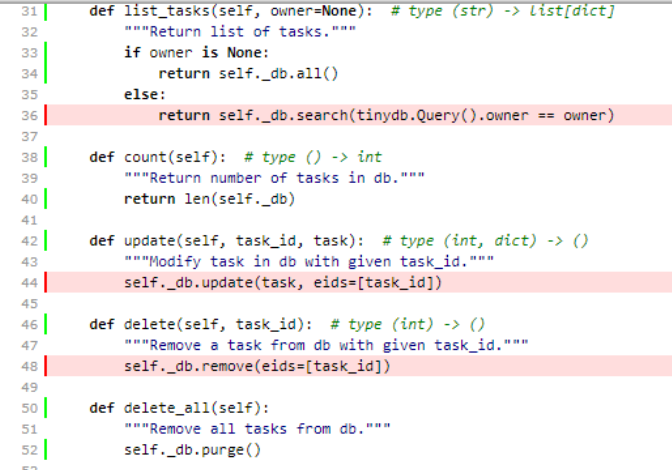
\includegraphics[scale=0.85]{figures/pytest_cov_html.png}
	\caption{ Страница html-отчета о покрытии кода тестами }\label{fig:pytest_cov_html}
\end{figure}

Из \pic{fig:pytest_cov_html} можно заключить, чт:
\begin{itemize}
	\item функция \texttt{list\_tasks} не тестируется для случая, когда задано имя владельца (эта строка отмечена красным),
	
	\item не тестируются функции \texttt{update} и \texttt{delete}.
\end{itemize}

Теперь можно эти функции включить в список TO-DO по тестированию вместе с тестированием системы конфигурации.

Хотя большой процент покрытия -- это хорошая цель, а инструменты тестирования полезны для получения информации о состоянии тестового покрытия, сама по себе величина процента не особо информативна.

Например, покрытие кода тестами на 100\% -- достойная цель, но это не обязательно означает, что код тестируется полностью. Эта величина лишь показывает, что все строки кода в программе выполнены, но не сообщает, что были протестированы все условия.

Кроме того, когда есть, который не тестируется, это может означать. что необходим тест. Но это также может означать, что есть некотрые функции системы, которые не нужны и могут быть удалены.

Стоит использовать информацию о покрытии с целью расширения набора тестов и создания их для кода, который не запускается. Это упрощает поддержку проекта и повышает общее качество кода.

\subsection{Виртуальные окружения}

Одно из главных применений виртуального окружения -- обеспечение чистого окружения для запуска модульных тестов.

Для тестирования приложений в различных средах удобно использовать \texttt{tox}. \texttt{tox} -- утилита командной строки, которая позволяет запускать полный набор тестов в нескольких средах (например, с различными версиями Python, или различными конфигурациями для различных операционных систем).

В общих чертах \texttt{tox} работает так
\begin{enumerate}
	\item Создает виртуальную среду в каталоге \texttt{.tox},
	
	\item Устанавливает некоторые зависимости,
	
	\item Устанавливает пакет из \texttt{sdist},
	
	\item Запускает тесты,
	
	\item Создает отчет с результатами.
\end{enumerate}

Для того чтобы включить в проект поддержку \texttt{tox}, нужно подготовить файл \texttt{tox.ini} на том же уровне, что и \texttt{setup.py}
\begin{lstlisting}[
style = bash,
numbers = none	
]
project/
  |-- setup.py
  |-- tox.ini
  ...
\end{lstlisting}

Конфигурационный файл \texttt{tox.ini} может выглядеть так
\begin{lstlisting}[
title = {\sffamily tox.ini},
style = bash,
numbers = none	
]
[tox]
envlist = py27,py36

[testenv]
deps=pytest  # если pytest нет в системе, то tox его установит
commands=pytest # запустит pytest внутри тестового окружения

[pytest]
addopts = -rsxX -l --tb=short --strict
markers = 
    smoke: Run the smoke test functions
    get: Run the test functions that test tasks.get()

\end{lstlisting}

Если запустить код сейчас, \texttt{tox} создаст окружение, установит новую зависимость и запустит команду \texttt{pytest}, котрая выполнит все модульные тесты. Для добавления новых зависимостей можно либо добавить их в опцию \texttt{deps} конфигурации, как в примере, либо воспользоваться \verb|-rfile| для чтения из файла.

Здесь строка \texttt{envlist = py27,py36} позволяет запускать тесты с использованием Python 2.7 и Python 3.6.

Строка \texttt{deps=pytest} заставляет \texttt{tox} проверить установлен ли \texttt{pytest}. Строка \texttt{commands=pytest} говорит \texttt{tox}, что нужно запускать \texttt{pytest} в каждой среде.

Строка \texttt{addopts = -rsxX} включает дополнительную сводную информацию для пропусков, а \texttt{-l} включает отображение локальных переменных в трассировке стека. Он также по умолчанию использует сокращенные трассировки стека (\verb|--tb=short|) и гарантирует, что все маркеры, используемые в тестах, будут объявлены первыми (\verb|--strict|). 

Можно запустить тесты и для другой версии Python, если передать метку \verb|-e| в \texttt{tox}, например
\begin{lstlisting}[
style = bash,
numbers = none
]
tox -e py26
\end{lstlisting}

По умолчанию \texttt{tox} имитирует любое окружение, которое совпадает со следующими версиями Python: \texttt{py24}, \texttt{py25}, \texttt{py26}, \texttt{py27}, \texttt{py30}, \texttt{py31}, \texttt{py32}, \texttt{py33}, \texttt{py34}, \texttt{py35}, \texttt{py36}, \texttt{py37}, \texttt{jython} и \texttt{pypy}.

Можно определить свои собственные окружения. Для этого достаточно добавить секцию с именем \texttt{[testenv:envname]}
\begin{lstlisting}[
style = bash,
numbers = none	
]
[testenv]
deps=pytest
commands=pytest

[testenv:py36-coverage]
deps=
    {[testenv]deps} # значение переменной deps из раздела [testenv]
    pytest-cov
commands=pytest --cov=myproject
\end{lstlisting}

Используя \verb|pytest --cov=myproject| на секции \texttt{py36-coverage}, как показано в примере, мы переопределили команды для окружения \texttt{py36-coverage}. Когда мы запустим \texttt{tox -e py36-coverage}, то установим \texttt{pytest} как одну из зависимостей, а сама команда \texttt{pytest} запуститься с опцией \texttt{coverage}.

Здесь мы заменили значение \texttt{deps} на аналогичное значение из \texttt{testenv} и добавили зависимость с \texttt{pytest-cov}.

В \texttt{tox} поддерживается интерполяция переменных, поэтому можно обращаться к любому полю из файла \texttt{tox.ini} и использовать его как переменную с помощью синтаксиса
\begin{lstlisting}[
style = bash,
numbers = none	
]
{[env_name]variable_name}
\end{lstlisting}


\section{Автоматическое тестирование в Python}

Для автоматического тестирования удобно использовать библиотеку \texttt{Hypothesis} \url{https://hypothesis.readthedocs.io/en/latest/}. Подходит для граничного тестирования

Hypothesis:
\begin{itemize}
	\item Работает перебором, поиск минимального примера,
	
	\item "Знает" об особенностях данных в Python,
	
	\item Поддерживает map,
	
	\item Подходит для тестирования кода, который работает с пользователем напрямую.
\end{itemize}

Можно тестировать модели.



\section{Инструменты автоматического форматирования, инспектирования и анализа кода}

Список обсуждаемых инструментов:
\begin{itemize}
	\item \texttt{Deepsource}, \texttt{Deepcode}, \texttt{Codacy}, 
	
	\item \texttt{flake8},
	
	\item \texttt{black},
	
	\item \texttt{pre-commit},
	
	
\end{itemize}

Выполнить автоматический анализ кода можно с помощью следующих инструментов на базе~AI:
\begin{itemize}
	\item Deepsource \url{https://deepsource.io/}: нужно просто зарегистрироваться, например, через git-репозиторий, а затем подключить свой репозиторий для анализа; после того, как будет сделан коммит, запуститься процедура анализа на платформе DeepSource (результаты ); в репозитории будет создан специальный конфигурационный файл \texttt{.deepsource.toml},
	
	\item Deepcode \url{https://www.deepcode.ai/},
	
	\item Codacy \url{https://www.codacy.com/}
\end{itemize}

Пример конфигурационного файла для автоматического анализа кода на базе Deepsource
\begin{lstlisting}[
title = {\sffamily .deepsource.toml},
style = bash,
numbers = none	
]
version = 1

test_patterns = [
  'tests/**'
]

exclude_patterns = [

]

[[analyzers]]
name = "python"
enabled = true
runtime_version = "3.x.x"

  [analyzers.meta]
  max_line_length = 79
\end{lstlisting}

Наиболее общий инструмент инспектирования кода (так называемые линтеры) -- \texttt{flake8}. Flake8 умеет работать не только с PEP8, но и с другими правилами (кроме того поддерживате пользовательские плагины).

Для автоматического форматирования кода из командной строки или как pre-commit hook удобно использовать \texttt{black} \url{https://black.readthedocs.io/en/stable/installation_and_usage.html}.

Инструмент \texttt{black} поддерживается \texttt{vim} \url{https://black.readthedocs.io/en/stable/editor_integration.html#vim}.

Проще всего установить \texttt{black} в Vim с помощью менеджера плагинов \texttt{Vundle}.

Сначала нужно прописать в конфигурационном файле \verb|~/.vimrc| следующую строку
\begin{lstlisting}[
title = {\sffamily ~/.vimrc},
style = bash,
numbers = none	
]
Plugin 'psf/black'
\end{lstlisting}

А затем в сеансе Vim нужно набрать \texttt{:PluginInstall}. 

Если возникнет ошибка конца строки <<E492: Not an editor command: \verb|^M|>>, то в директории плагина (например, \directory{Users>leor.finkelberg>.vim>bundle>black}) можно воспользоваться конструкцией 
\begin{lstlisting}[
style = bash,
numbers = none	
]
# переконвертировать все vim-файлы в unix-формат
find . -name '*.vim' | xargs dos2unix -f
\end{lstlisting}

Утилита командной строки (и pre-commit hook) \texttt{yesqa} \url{https://pypi.org/project/yesqa/} используется для автоматического удаления ненужных комментариев вида \verb|# noqa|.

Для того чтобы перед коммитом \texttt{yesqa} проверяла код требуется включить в конфигурационный файл \texttt{.pre-commit-config.yaml} следующие строки
\begin{lstlisting}[
title = {\sffamily .pre-commit-config.yaml},
style = bash,
numbers = none	
]
...
-   repo: https://github.com/asottile/yesqa
    rev: v1.2.2
    hooks:
-   id: yesqa
...
\end{lstlisting}

Вот сложный пример \texttt{.pre-commit-config.yaml}

\begin{lstlisting}[
title = {\sffamily .pre-commit-config.yaml},
style = bash,
numbers = none	
]
exclude: _pb2\.py$
repos:
- repo: https://github.com/pre-commit/mirrors-isort
rev: f0001b2  # Use the revision sha / tag you want to point at
hooks:
- id: isort
args: ["--profile", "black"]
- repo: https://github.com/psf/black
rev: 20.8b1
hooks:
- id: black
- repo: https://github.com/asottile/yesqa
rev: v1.1.0
hooks:
- id: yesqa
additional_dependencies:
- flake8-bugbear==20.1.4
- flake8-builtins==1.5.2
- flake8-comprehensions==3.2.2
- flake8-tidy-imports==4.1.0
- flake8==3.7.9
-   repo: https://github.com/pre-commit/pre-commit-hooks
rev: v2.3.0
hooks:
- id: check-docstring-first
- id: check-json
- id: check-merge-conflict
- id: check-yaml
- id: debug-statements
- id: end-of-file-fixer
- id: trailing-whitespace
- id: flake8
- id: requirements-txt-fixer
-   repo: https://github.com/pre-commit/mirrors-pylint
rev: d230ffd
hooks:
-   id: pylint
args:
- --max-line-length=119
- --ignore-imports=yes
- -d duplicate-code
- repo: https://github.com/asottile/pyupgrade
rev: v2.7.3
hooks:
- id: pyupgrade
args: ['--py37-plus']
- repo: https://github.com/pre-commit/pygrep-hooks
rev: v1.5.1
hooks:
- id: python-check-mock-methods
- id: python-use-type-annotations
- repo: https://github.com/pre-commit/mirrors-mypy
rev: 9feadeb
hooks:
- id: mypy
args: [--ignore-missing-imports, --warn-no-return, --warn-redundant-casts, --disallow-incomplete-defs]
\end{lstlisting}

Перед коммитом полезно выполнять команду
\begin{lstlisting}[
style = bash,
numbers = none	
]
pre-commit run --all-files
\end{lstlisting}

ВАЖНО: если виртуальное окружение конструируется с помощью \texttt{conda} может возникнуть ошибка <<FileNotFoundError: [Errno 2] No such file or directory...>> \\ при запуске \verb|pre-commit run --all-files|.

Поэтому следует использовать \texttt{virtualenv} версии 20.0.33 (!)
\begin{lstlisting}[
style = bash,
numbers = none	
]
$ pip install virtualenv==20.0.33
$ virtualenv env
$ source env/bin/actiavte # для Linux/MacOs etc
$ env\Scripts\activate.bat # для Windows
\end{lstlisting}


\section{Тонкости импортирования модулей и пакетов в Python}

ОЧЕНЬ ВАЖНО: при импорте \emph{модуля} Python выполняет \emph{весь} код в этом модуле
\begin{lstlisting}[
style = bash,
numbers = none	
]
import something_module  # весь код модуля выполнился
\end{lstlisting}

ОЧЕНЬ ВАЖНО: при импорте \emph{пакета} Python выполняет модуль \verb|__init__.py| этого пакета и импортированные имена становятся частью пространства имен пакета
\begin{lstlisting}[
style = bash,
numbers = none	
]
import something_package  # выполнился модуль __init__.py этого пакета
\end{lstlisting}

Пример. Пусть структура пакетов выглядит так
\begin{lstlisting}[
style = bash,
numbers = none	
]
root_dir/
|-- packageA/
    |-- __init__.py  # from packageA import moduleA
    |                # from packageA import packageB
    |                # from packageA import foo
    |-- moduleA.py   # здесь объявлена функция mainA()
    |-- packageB/
    |   |-- __init__.py  # from packageA.packageB import moduleB
    |   |-- moduleB.py   # здесь объявлена функция mainB()
    |-- foo.py
\end{lstlisting}

То есть в модуле \verb|__init__.py| пакета \texttt{packageA} лежит такой код
\begin{lstlisting}[
title = {\sffamily packageA/\_\_init\_\_.py},
style = bash,
numbers = none	
]
# используются абсолютные пути от корня директории, из-под которой запускается
# интерактивная Python-сессия или базовый Python-сценарий
from packageA import moduleA
from packageA import packageB
from packageA import foo
\end{lstlisting}

Другими словами, при импорте пакета \texttt{packageA} будет выполнен модуль \verb|__init__.py|, который добавит в пространство имен пакета имена \texttt{moduleA}, \texttt{packageB} и \texttt{foo}. Это означает, что эти модули и пакет будут доступны через обращение к пакету \texttt{packageA}
\begin{lstlisting}[
style = bash,
numbers = none	
]
import packageA

packageA.foo
packageA.moduleA
packageA.packageB
\end{lstlisting}

Убедится в том, что при запуске главного сценария из-под корневой директории будут доступны для импорта через имя пакета \texttt{packageA} имена \texttt{moduleA}, \texttt{packageB} и \texttt{foo} можно так
\begin{lstlisting}[
title = {\sffamily вызов из-под корневой директории},
style = bash,
numbers = none
]
import pkgutil

list(pkgutil.iter_modules(["./packageA"]))
# [ModuleInfo(module_finder=FileFinder('./packageA'), name='foo', ispkg=False),
# ModuleInfo(module_finder=FileFinder('./packageA'), name='moduleA', ispkg=False),
# ModuleInfo(module_finder=FileFinder('./packageA'), name='packageB', ispkg=True)]
\end{lstlisting}

Функцию \texttt{pkgutil.iter\_modules(path=search\_path)} можно использовать, чтобы получить список всех модулей/пакетов, которые можно импортировать по заданному пути.

При импорте пакета \texttt{packageB} аналогично будет выполнен модуль \texttt{\_\_init\_\_.py} этого пакета
\begin{lstlisting}[
title = {\sffamily packageA/packageB/\_\_init\_\_.py},
style = bash,
numbers = none	
]
# используются абсолютные пути от корня директории, из-под которой запускается
# интерактивная Python-сессия или базовый Python-сценарий
from packageA.packageB import moduleB
\end{lstlisting}

Таким образом, модуль \texttt{moduleB} становится частью пространства имен пакета \texttt{packageB}. То есть при импорте пакета \texttt{packageB} к модулю \texttt{moduleB} можно будет обраться так
\begin{lstlisting}[
style = bash,
numbers = none	
]
import pkgutil

import packageA.packageB as pkB

pkB.moduleB
list(pkgutil.iter_modules(["./packageA/packageB"]))
# [ModuleInfo(module_finder=FileFinder('./packageA/packageB'), name='moduleB', ispkg=False)]
\end{lstlisting}

Первым элементом списка путей \texttt{sys.path} будет директория, в которой лежит выполняемый Python-сценарий.

Python ищет модули в следующем порядке
\begin{itemize}
	\item Модули стандартной библиотеки (например, \texttt{math}, \texttt{os} etc.),
	
	\item Модули/пакеты, указанные в \texttt{sys.path}:
	\begin{itemize}
		\item Если интерпретатор запущен в интерактивном режиме:
		\begin{itemize}
			\item \texttt{sys.path[0]} -- пустая строка, \verb|""|. Это значит, что Python будет искать в текущей директории, из-под которой был запущен интерпретатор,
		\end{itemize}
	
	    \item Если сценарий был запущен командой \texttt{python <script.py>}:
	    \begin{itemize}
	    	\item \texttt{sys.path[0]} -- это путь к \texttt{<script.py>}.
	    \end{itemize}
	\end{itemize}

    \item Директории, указанные в переменной среды \texttt{PYTHONPATH},
    
    \item Директория по умолчанию, которая зависит от дистрибутива Python.
\end{itemize}

\remark{%
При запуске сценария для \texttt{sys.path} важна не директория, из-под которой запускается сценарий, а \emph{путь к самому сценарию}
}

{\color{red}ОЧЕНЬ ВАЖНО: \texttt{sys.path} в качестве текущей директорией проекта назначает ту, \emph{в которой} размещается запускаемый Python-сценарий, а библиотека \texttt{pathlib2} -- \emph{корень} проекта!!!}

У модуля \verb|__init__.py| есть две функции:
\begin{itemize}
	\item Превратить папку со скриптами в импортируемый пакет модулей (до версии Python 3.3, в версиях Python 3.3+ в этом нет необходимости, так как все директории по умолчанию считаются пакетами),
	
	\item Выполнить код инициализации пакета.
\end{itemize}

Чтобы импортировать модуль/пакет из директории, которая находится не в директории запущенного сценария, этот модуль/пакет должен быть в пакете.

В момент, когда пакет или один из его модулей импортируется в первый раз, Python выполняет \verb|__init__.py| в корне пакета, если такой файл существует. Все объекты, определенные в \verb|__init__.py|, считаются частью пространства имен пакета.

\remark{%
Если Python-сценарий запускается из-под пакета (директории, содержащей или не содержащей модуля \texttt{\_\_init\_\_.py}), то модуль \texttt{\_\_init\_\_.py} этого пакета не вызывается, так как директория, в которой находится сценарий \emph{пакетом не считается}
}

При \emph{абсолютном} импорте используется полный путь от начала корневой папки проекта к нужному модулю.

При \emph{относительном} импорте используется относительный путь, начиная с местоположения текущего модуля и заканчивая местоположением интересующего модуля.

\remark{%
Как правило, рекомендуется использовать абсолютный импорт
}

\section{Логистическая функция потерь}

\href{https://dyakonov.org/2018/03/12/логистическая-функция-ошибки/}{\emph{Логистическую функцию потерь}} (logloss) еще называют \emph{перекрестной энтропией} и часто используют в задачах классификации.

Функция ошибки называется \href{https://dyakonov.org/2020/12/28/proper-scoring-rules/}{\emph{скоринговой}} (proper scoring rules), если
\begin{align*}
	p = \argmin \mathbf{E}_y \,L(y, a), \ y \sim Bernoulli(p),
\end{align*}
то есть оптимальный ответ на каждом объекте -- его вероятность принадлежности к классу 1. Например, логистическая функция потерь является скоринговой. Сама теория скоринговых функций является самостоятельным направлением в теории вероятностей и математической статистики.

Функцию ошибки MSE в задачах классификации называют <<ошибкой Брайера>> (Brier score), именно под таким названием она реализована в \texttt{scikit-learn}
\begin{lstlisting}[
style = ironpython,
numbers = none	
]
from sklearn.metrics import brier_score_loss
brier_score_loss(y_true, y_prob)
\end{lstlisting}


\section{Приемы распараллеливания приложений с \\библиотекой \texttt{concurrent.futures}}

Future-объекты в Python (как и, в частности, в Scala) инкапсулируют ожидающие операции. 

ЗАМЕЧАНИЕ: в Python Future-объекты не должны создаваться пользователем! Предполагается, что эти объекты создает библиотека.

Пример организации работы многопотчного приложения
\begin{lstlisting}[
style = ironpython,
numbers = none	
]
# пул из 10 потоков
with ThreadPoolExecutor(max_workers=10) as executor:
    path_iterdir = pathlib2.Path(".").iterdir() # генератор
    paths_to_csv_files = ( # генератор
        path for path in path_iterdir if path.suffix == ".csv"
    )
    collection_of_futures = (
        executor.submit(count_lines, path_to_file) # submit возвращает Future-объект
        for path_to_file in paths_to_csv_files
    )
    
    # возвращает результаты в порядке готовности
    for future in futures.as_completed(collection_of_futures):
        print(future.result())
\end{lstlisting}

ЗАМЕЧАНИЕ: \texttt{executor.map} запоминает порядок вызова. То есть, если первой вызванной функции потребовалось 10 сек на получение результата, а всем остальным по 1 сек., то программа будет заблокированна на 10 сек., поскольку она пытается получить первый результат генератора, возвращенного функцией \texttt{map}. После этого все остальные результаты будут получены без блокировки, потому что соответствующие функции уже завершились.

Однако, часто предпочтительнее получать результаты по мере их готовности вне зависимости от того, в каком порядке подавались задачи. Для этого потребуется комбинация метода \texttt{executor.submit} и функции \texttt{futures.as\_completed}.

Комбинация \texttt{executor.submit} и \texttt{futures.as\_completed} обладает большей гибкостью, чем \texttt{executor.map}, потому что ей можно подавать различные вызываемые объекты и аргументы, тогда как \texttt{executor.map} предназначен для выполнения одного и того же вызываемого объекта с разными аргументами.

Кроме того, множество будущих объектов, передаваемых \texttt{futures.as\_completed}, может поступать от нескольких исполнителей -- одни из них могли быть созданы экземпляром \texttt{ThreadPoolExecutor}, другие -- экземпляром \texttt{ProcessPoolExecutor}.


\section{Автоматический анализ кода с платформой DeepsSource}

Платформа DeepSource \url{https://deepsource.io/} позволяет проводить автоматический анализ кода на анти-паттерны, проблемы с производительностью и поиск уязвимостей при каждом коммите или pull-request. Кроме того платформа отслеживает количество зависимостей, покрытие документацией и пр.

С документацией можно ознакомиться здесь \url{https://deepsource.io/docs/}.

Управлять поведением DeepSource можно с помощью конфигурационного \\файла \texttt{.deepsource.toml}
\begin{lstlisting}[
title = {\sffamily .deepsource.toml},
style = bash,
numbers = none	
]
version = 1

test_patterns = [
    "tests/**",
    "test_*.py"
]

exclude_patterns = [
    "migrations/**",
    "**/examples/**"
]

[[analyzers]]
name = "python"  # анализатор для Python
enabled = true
dependency_file_paths = ["requirements/development.txt"] # список внешних зависимостей

    [analyzers.meta]  # метаданные для анализатора
    runtime_version = "3.x.x" # версия языка
    type_checker = "mypy" # анализатор проверки типов
    max_line_length = 79  # максимально допустимая длина строки
    skip_doc_coverage = ["module", "magic", "init"] # артифакты, которые следует пропустить при расчете покрытия документации
    additional_builtins = ["_", "pretty_output"] # дополнительные модули
    
[[analyzers]]
name = "shell"  # анализатор для сценариев командной оболочки
enabled = true

    [analyzers.meta]
    dialect = "zsh"

[[analyzers]]  # анализатор для SQL
name = "sql"
enabled = true

    [analyzers.meta]
    max_line_length = 100
    tab_space_size = 4
    indent_unit = "tab"
    comma_style = "trailing"
    capitalisation_policy = "consistent"
    allow_scalar = true
    single_table_references = "consistent"
\end{lstlisting}

По умолчанию, если в репозитории обнаруживаются ниже перечисленные файлы, то они проверяются на наличие зависимостей
\begin{itemize}
	\item \texttt{Pipfile},
	
	\item \texttt{Pipfile.lock},
	
	\item \texttt{poetry.lock},
	
	\item \texttt{pyproject.toml} (если содержит разделы \texttt{[tool.poetry]} или \texttt{[tool.fit]}),
	
	\item \texttt{requirements.txt},
	
	\item \texttt{setup.py}.
\end{itemize}

Файл \texttt{.deepsource.toml} располагается в корне проекта
\begin{lstlisting}[
style = bash,
numbers = none	
]
.
|-- .deepsource.toml
|-- README.md
|-- bar
|   |-- baz.py
|-- foo.py
\end{lstlisting}

Вот исчерпывающий список возможных вариантов конфигурации
\begin{itemize}
	\item \texttt{version}: обязательное свойство; на текущий момент поддерживается только значение <<1>>
\begin{lstlisting}[
style = bash,
numbers = none	
]
version = 1
\end{lstlisting}
	
	\item \texttt{exclude\_patterns}: список шаблонов файлов и директорий, которые не должны учитываться при выполнении анализа; шаблоны строятся относительно корня проекта
\begin{lstlisting}[
style = bash,
numbers = none
]
exclude_patterns = [
    "bin/**",
    "**/node_modules/",
    "js/*/*/min.js"
]
\end{lstlisting}
	
	\item \texttt{test\_patterns}: список шаблонов файлов и директорий, содержащих тестовые файлы; шаблоны строятся относительно корня проекта,
\begin{lstlisting}[
style = bash,
numbers = none	
]
test_patterns = [
    "tests/**",
    "test_*.py"
]
\end{lstlisting}
	
	\item \texttt{analyzers}: список анализаторов (в конфигурации должен быть хотя бы один анализатор),
\begin{lstlisting}[
style = bash,
numbers = none	
]
[[analyzers]]
name = "python"
enabled = true
dependency_file_paths = [
    "requirements.txt",
    "Pipfile"
]
\end{lstlisting}
	
	\item \texttt{transformers}: список трансформеров
\begin{lstlisting}[
style = bash,
numbers = none	
]
[[transformers]]
name = "black"
enabled = true
\end{lstlisting}
\end{itemize}

\subsection{Связка DeepSource и Travis CI}

Для того чтобы платформа DeepSource имела возможность извлекать метрики покрытия кода тестами из Travis CI \url{https://www.travis-ci.com/} следует в конфигурационный \\файл \texttt{.deepsource.toml} добавить анализатор <<Test Coverage>> (см. \url{https://deepsource.io/docs/how-to/add-python-cov-ci.html})
\begin{lstlisting}[
title = {\sffamily .deepsource.toml},
style = bash,
numbers = none	
]
...
[[analyzers]]
name = "test-coverage"
enabled = true
...
\end{lstlisting}
а в конфигурационный файл \texttt{.travis.yml} следующие строки
\begin{lstlisting}[
title = {\sffamily .travis.yml},
style = bash,
numbers = none	
]
# Travis CI config
...
after_success:  # this is for DeepSource.io
  # Generate coverage report in xml format
  - coverage xml

  # Install deepsource CLI
  - curl https://deepsource.io/cli | sh

  # From the root directory, run the report coverage command
  - ./bin/deepsource report --analyzer test-coverage --key python --value-file ./coverage.xml
\end{lstlisting}

Затем на странице Travis CI, на вкладке Settings, например, \url{https://www.travis-ci.com/github/LeorFinkelberg/termostablizator/settings}, необходимо создать переменную окружения \texttt{DEEPSOURCE\_DSN} со значением Data Source Name (DNS), которое можно узнать на странице DeepSource по пути \directory{Settings > Reporting}.

Получится что-то вроде
\begin{lstlisting}[
style = bash,
numbers = none
]
DEEPSOURCE\_DSN=https://0a69347b13674f13a8ca39b9464cb682@deepsource.io
\end{lstlisting}




\section{\texttt{Python} и \LaTeX}

Для компиляции \LaTeX-документов прямо из-под \texttt{Python} можно использовать библиотеку \texttt{pylatex}\footnote{Устанавливается как обычно \texttt{pip install pylatex}} \url{https://jeltef.github.io/PyLaTeX/current/}.

\section{EM-алгоритм и разделение смеси распределений}

EM-алгоритм -- алгоритм нахождения \emph{оценок максимального правдоподобия} параметров вероятностных моделей со \emph{скрытыми переменными}\footnote{Скрытые переменные -- переменные, которые не могут быть измерены в явном виде, а могут только быть выведены через математические модели с использованием наблюдаемых переменных}. На E-шаге (expectation) вычисляется ожидаемое значение \emph{функции правдоподобия}, при этом скрытые переменные рассматриваются как наблюдаемые. На M-шаге (maximization) вычисляется оценка максимального правдоподобия, таким образом увеличивается ожидаемое правдоподобие, вычисляемое на E-шаге. Затем значение используется для E-шаге на следующей итерации. Алгоритм выполняется до сходимости.

EM-алгоритм итеративно улучшает начальную оценку $ \Theta_0 $, вычисляя новые значения оценок $ \Theta_1 $, $ \Theta_0 $ и так далее. На каждом шаге переход к $ \Theta_{n + 1} $ от $ \Theta_n $ выполняется следующим образом
\begin{align*}
	\Theta_{n + 1} = \underset{\Theta}{\arg \max}\, Q(\Theta),
\end{align*}
где $ Q(\Theta) $ -- матожидание логарифмической функции правдоподобия.

$ Q(\Theta) $ вычисляется следующим образом
\begin{align*}
	Q(\Theta) = \mathbf{E} \big[ \log p(X, T | \Theta) | X \big]
\end{align*}
то есть это условное матожидание при условии X.


В тех случаях, когда <<форму>> класса не удается описать каким-либо одним распределением, можно попробывать описать ее смесью распределений.

Плотность распределения на $ X $ имеет вид смеси $ k $ распределений
\begin{align*}
	p(x) = \sum_{j=1}^{k} w_j p_j(x), \quad \sum_{j=1}^{k} w_j = 1, \quad w_j \geqslant 0,
\end{align*}
где $ p_j(x) $ -- функция правдоподобия $ j $-ой компоненты смеси, $ w_j $ -- ее априорная вероятность.

Функции правдоподобия принадлежат параметрическому семейству распределений $ \varphi(x; \theta) $ и отличаются только значениями параметра $ p_j(x) = \varphi(x; \theta_j) $.

Иными словами, <<выбрать объект $ x $ из смеси $ p(x) $>> означает сначала выбрать $ j $-ую компоненту смеси из дискретного распределения $ \{w_1, \ldots, w_k\} $, а затем выбрать объект $ x $ согласно плотности $ p_j(x) $.

\emph{Функция правдоподобия} -- совместная плотность распределения вероятностей $ f_{X_1, \ldots, X_n}(x_1, \ldots, x_n; \theta) $ случайных величин $ X_1, \ldots, X_n $, рассматриваемых как функция параметра $ \theta $ при фиксированной реализации $ (x_1, \ldots, x_n) $ выборки $ X_1, \ldots, X_n $. Для рассматриваемой параметрической модели случайные величины $ X_1, \ldots, X_n $ \underline{независимы} и \underline{одинаково распределены}, поэтому \emph{функция правдоподобия} записывается в виде \cite{shulenin-ch1}
\begin{align*}
	L(x_1, \ldots, x_n; \theta) = f_{X_1, \ldots, X_n}(x_1, \ldots, x_n; \theta) = \prod_{i=1}^{n} f_X(x_i; \theta).
\end{align*}

Отметим, что логарифм функции правдоподобия, то есть
\begin{align*}
	\ln L(\vec{x}, \theta) = \sum_{i=1}^{n} \ln f_X(x_i; \theta),
\end{align*}
часто называют \emph{логарифмической функцией правдоподобия}.

Таким 

Задача разделения смеси заключается в том, чтобы, имея выборку $ X^m $ случайных и независимых наблюдений из смеси $ p(x) $, зная число $ k $ и функцию $ \varphi $, оценить вектор параметров $ \Theta = (w_1, \ldots, w_k, \theta_1, \ldots, \theta_k) $.

К сожалению, попытка разделить смесь, используя принцип максимума правдоподобия <<в лоб>>, приводит к слишком громоздкой оптимизационной задаче. Обойти эту трудность позволяет EM-алгоритм (expection-maximization). Идея алгоритма заключается в следующем. Искусственно вводится вспомогательный вектор \emph{скрытых} переменных $ G $, обладающий двумя замечательными свойствами. С одной стороны, он может быть вычислен, если известны значения вектора параметров $ \Theta $, а с другой, поиск максимума правдоподобия сильно упрощается, если известны значения скрытых переменных.

EM-алгоритм состоит из итерационного повторения двух шагов:
\begin{itemize}
	\item на E-шаге вычисляется ожидаемое значение (expectation) \emph{вектора скрытых переменных} $ G $ по текущему приближению \emph{вектора параметров} $ \Theta $,
	
	\item на M-шаге решается задачи максимизации правдоподобия (maximization) и находится следующее приближение вектора параметров $ \Theta $ по текущим значениям векторов $ G $ и $ \Theta $.
\end{itemize} 

То есть
\begin{algorithmic}[1]
	\STATE Вычислить начальное приближение вектора параметров $ \Theta $;
	\REPEAT
	    \STATE $ G := \text{E-step}(\Theta) $;
	    \STATE $ \Theta := \text{M-step}(\Theta, G) $;
	\UNTIL{$ \Theta $ и $ G $ не стабилизируются.}
\end{algorithmic}

Область EM-алгоритма чрезвычайно широка -- дискриминантный анализ, кластеризация, восстановление пропусков в данных, обработка сигналов и изображений. Здесь мы рассмотрим его как инструмент разделения смеси распределений.

\emph{\bfseries E-шаг (expectation)}. Обозначим через $ p(x, \theta_j) $ плотность вероятности того, что объект $ x $ получен из $ j $-ой компоненты смеси. По формуле условной вероятности $ p(x, \theta_j) = p(x) \mathbf{P}(\theta_j | x) = w_j p_j(x) $.

Введем обозначение $ g_{ij} \equiv \mathbf{P}(\theta_j | x_i) $. Это \emph{неизвестная апостериорная} вероятность того, что обучающий объект $ x_i $ получен из $ j $-ой компоненты смеси. Возьмем эти величины в качестве \emph{скрытых переменных}. Обозначим $ G = (g_1, \ldots, g_j) $, где $ g_j $ -- $ j $-ый столбец матрицы $ G $. Каждый экземпляр обучающего набора данных обязательно принадлежит какой-то компоненте, поэтому справедлива формула полной вероятности
\begin{align*}
	\sum_{j=1}^{k} g_{ij} = 1, \quad \forall i = 1, \ldots, l.
\end{align*}

Зная параметры компонент $ w_j $, $ \theta_j $, легко вычислить $ g_{ij} $ по формуле Байеса
\begin{align*}
	g_{ij} = \dfrac{ w_j p_j(x_j) }{ \sum_{s=1}^{k} w_s p_s(x_i) }, \quad \forall i, j.
\end{align*}

В этом и заключается E-шаг EM-алгоритма.

\emph{\bfseries M-шаг (maximization)}. Покажем, что знание значений скрытых переменных $ g_{ij} $ и принцип максимума правдоподобия приводит к оптимизационной задаче, допускающей эффективное численное (или даже аналитическое) решение. Будем максимизировать логарифм правдоподобия
\begin{align*}
	Q(\Theta) = \ln \prod_{i=1}^{m} p(x_i) = \sum_{i=1}^{m} \ln \sum_{j=1}^{k} w_j p_j(x_i) \to \underset{\Theta}{\max}
\end{align*}
при ограничении $ \sum\limits_{j=1}^{k} w_j = 1 $.

Таким образом, M-шаг сводится к вычислению весов компонент $ w_j $ и оцениванию параметров компонент $ \theta_j $ путем решения $ k $ независимых оптимизационных задач. Отметим, что разделение переменных оказалось возможным благодаря удачному введению скрытых переменных.

\emph{Критей останова}. Итерации останавливаются, когда значения функционала $ Q(\Theta) $ или скрытых переменных $ G $ перестают существенно изменяться. Удобнее контролировать скрытые переменные, так как они имеют смысл вероятностей и принимают значения из отрезка $ [0, 1] $.

\section{Адаптивный бустинг}

В лекции К.В. Воронцова \url{https://www.youtube.com/watch?v=5QrWW_ZlP9w&list=PLJOzdkh8T5krxc4HsHbB8g8f0hu7973fK&index=15} говорится, что алгоритм адаптивного бустинга использует 3 значения целевой переменной: -1, +1 и 0 (отказ базового алгоритма от классификации). То есть если алгоритм не уверен в ответе, его вес будет равен 0, и, следовательно, прогнозы такого алгоритма не будут учитываться при взвешенном голосовании.

ЗАМЕЧАНИЕ: адаптивный бустинг строит <<черные ящики>> -- громоздкие неинтерпретируемые композиции из сотен алгоритмов.

\subsection{Фильтрация выбросов}

После построения некоторого количества базовых алгоритмов (скажем, пары десятков) имеет смысл проанализировать распределение весов объектов. Объекты с наибольшими весами wi, скорее всего, являются шумовыми выбросами, которые стоит исключить из выборки, после чего начать построение композиции заново. Вообще, бустинг можно использовать как универсальный \emph{метод фильтрации выбросов} перед применением любого другого метода классификации.

\subsection{Достоинства и недостатки адаптивного бустинга}

Достоинства AdaBoost:
\begin{itemize}
	\item Хорошая обобщающая способность. В реальных задачах (не всегда, но часто)
	удаётся строить композиции, превосходящие по качеству базовые алгоритмы.
	Обобщающая способность может улучшаться (в некоторых задачах) по мере
	увеличения числа базовых алгоритмов.
	
	\item Простота реализации.
	
	\item Накладные расходы бустинга невелики. Время построения композиции прак-
	тически полностью определяется временем обучения базовых алгоритмов.
	
	\item Возможность идентифицировать выбросы. Это наиболее <<трудные>> объекты $ x_i $,
	для которых в процессе наращивания композиции веса $ w_i $ принимают наибольшие значения.
\end{itemize}

Недостатки AdaBoost:
\begin{itemize}
	\item AdaBoost \emph{\color{red}склонен к переобучению} при наличии значительного уровня \emph{шума в данных}. Экспоненциальная функция потерь слишком сильно увеличивает веса <<наиболее трудных>> объектов, на которых ошибаются многие базовые алгоритмы. Однако именно эти объекты чаще всего оказываются шумовыми выбросами. В результате AdaBoost начинает настраиваться на шум, что ведёт к переобучению. Проблема решается путём удаления выбросов или применения менее <<агрессивных>> функций потерь. В частности, алгоритм LogitBoost использует логистическую функцию.
	
	\item AdaBoost требует достаточно длинных обучающих выборок. Другие методы
	линейной коррекции, в частности, бэггинг, способны строить алгоритмы сопоставимого качества по меньшим выборкам данных.
	
	\item Жадная стратегия последовательного добавления приводит к построению
	неоптимального набора базовых алгоритмов. Для улучшения композиции можно периодически возвращаться к ранее построенным алгоритмам и обучать их
	заново. Для улучшения коэффициентов $ \alpha_t $ можно оптимизировать их ещё раз по окончании процесса бустинга с помощью какого-нибудь стандартного метода построения линейной разделяющей поверхности. Рекомендуется использовать для этой цели SVM -- машины опорных векторов.
	
	\item Бустинг может приводить к построению громоздких композиций, состоящих
	из сотен алгоритмов. Такие композиции исключают возможность содержательной интерпретации, требуют больших объёмов памяти для хранения базовых
	алгоритмов и существенных затрат времени на вычисление классификаций.
\end{itemize}


\subsection{Адаптивный бустинг широкими мазками}

Бустинг является одной из самых мощных идей машинного обучения. Первоначально он был разработан для задач \emph{классификации}, но, его можно распространить и на \emph{регрессию}. Цель бустинга -- создание процедуры, которая объединяет результаты многих слабых классификаторов для создания мощного комитета.

Проблема переобучения в случае адаптивного бустинга выражена не так явно, как, например, в случае простых деревьев принятия решений, так как для того чтобы модель могла переобучиться у нее должно быть достаточное число степеней свободы (т.е. модель должна быть достаточно сложной), а мета-классификатор в адаптивном бустинге строится, как правило, на очень простых моделях, которые не могут <<запомнить>> всех особенностей данных.

Слабым классификатором является тот, уровень ошибок которого ненамного лучше случайного угадывания. Цель бустинга состоит в том, чтобы последовательно применять алгоритм слабой классификации к многократно измененным версиям данных, тем самым создавая последовательность слабых классификаторов $ G_m(x), m = 1, \ldots, M $. Прогнозы, полученные от всех этих классификаторов, затем объединяются, и окончательное решение принимается по взвешенному большинству голосов
\begin{align*}
	G(x) = \text{sign} \big( \sum_{m=1}^{M} \alpha_m G_m(x) \big)
\end{align*}

Здесь коэффициенты $ \alpha_1, \alpha_2, \ldots, \alpha_M $ рассчитываются с помощью алгоритма бустинга и взвешивают вклад каждого соответствующего классификатора $ G_m(x) $. Их эффект состоит в том, чтобы придать больший вес более точным классификаторам, входящим в последовательность.

Модификации данных на каждом этапе бустинга состоят из применения весов $ w_1, w_2, \ldots, w_N $ к каждому обучающему наблюдению $ (x_i, y_i), i = 1, 2, \ldots, N $. Первоначально все веса установлены равными $ w_i = 1/N $, так что первый шаг обучает классификатор на данных обычным способом. Для каждой последующей итерации $ m = 2, 3, \ldots, M $ веса наблюдений модифицируются индивидуально, и к взвешенным наблюдениям применяется алгоритм классификации. На этапе $ m $ те наблюдения, которые были неправильно классифицированы классификатором $ G_{m-1}(x) $, созданном на предыдущем этапе, получают повышенные веса, тогда как веса тех наблюдений, которые были классифицированы правильно, уменьшаются.

Таким образом, по мере продолжения итераций наблюдения, которые \emph{трудно} правильно классифицировать, получают все б\emph{о}льшее влияние. Следовательно, каждый последующий классификатор вынужден концентрироваться на тех \emph{обучающих} наблюдениях, которые пропущены предыдущими классификаторами, входящими в последовательность.

Алгоритм адаптивного бустинга
\begin{enumerate}
	\item Инициализируем веса экземпляров обучающего набора данных $ w_i = 1/N, i = 1, 2, \ldots, N $,
	
	\item Для $ m = 1 $ до $ M $
	\begin{enumerate}
		\item Настраиваем классификатор $ G_m(x) $ на обучающих данных, используя веса $ w_i $,
		
		\item Вычисляем
\begin{align*}
	err_m = \dfrac{ \sum\limits_{i=1}^{N} w_i I\big(y_i \neq G_m(x_i)\big) }{ \sum\limits_{i=1}^{N} w_i}
\end{align*}

        \item Вычисляем вес классификатора-примитива
\begin{align*}
	\alpha_m = \dfrac{1}{2} \log \dfrac{ 1- err_m }{ err_m },
\end{align*}

        \item Обновляем
\begin{align*}
	w_i \leftarrow w_i \cdot \exp \{ \alpha_m \cdot I(y_i \neq G_m(x_i)) \}, \ i = 1, 2, \ldots, N
\end{align*}
	\end{enumerate}

    \item Выводим результат
\begin{align*}
	G(x) = \text{sign} \big[ \sum_{m=1}^{M} \alpha_m G_m(x) \big].
\end{align*}
\end{enumerate}

Здесь $ i $ -- индекс экземпляра обучающего набора данных; $ m $ -- индекс классификатора.

ВАЖНО: одноуровневые деревья решений (пеньки решений) в случае \emph{взвешенной выборки} строятся как обычно, с отбором признаков и пороговых значений на основании метрик качества разбиения родительского узла (например, на основании информационного прироста, вычисленного по загрязненности Джини или энтропии Шеннона), но вместо вычисления отношения числа экземпляров $ k $-ого класса к общему числу экземпляров, попавших в рассматриваемый лист, оперировать приходится весами этих экземпляров.

\subsection{Обучение на взвешенной выборке}

Отличная лекция Разинкова \url{https://www.youtube.com/watch?v=jjwH1qn_C0k}.

Целевая функция для \emph{регрессии} на взвешенной выборке вычисляется как
\begin{align*}
	E(\theta) = \dfrac{1}{2} \sum_{i=1}^{N} w_i (t_i - y(\mathbf{x}_i, \theta))^2,
\end{align*}
а для классификации -- как
\begin{align*}
	E(\theta) = - \sum_{i=1}^{N}w_i \sum_{k=1}^{K} t_i^{(k)}\ln {y}(\mathbf{x}_i, \theta).
\end{align*}

Информационный прирост на деревьях решений по \emph{взвешенной выборке} определяется как
\begin{align*}
	I_w = H_w(S_i) - \sum_{i} \dfrac{\tilde{N}_{ij}}{\tilde{N}_i} H_w(S_{ij}), \quad H_w(S_i) = - \sum_k \dfrac{\tilde{N}_i^{(k)}}{\tilde{N}_i} \log \dfrac{\tilde{N}_i^{(k)}}{\tilde{N}_i},
\end{align*}
здесь $ i $ -- индекс родительского узла; $ j $ -- индекс дочернего узла; $ k $ -- индекс класса; $ \tilde{N}_i = \sum\limits_{x_l \in S_i} w_l $ -- это не количество экземпляров, попавших в рассматриваемый узел, а \emph{сумма их весов}.



\subsection{Основные концепции адаптивного бустинга. Разбор видео-лекции Josh Starmer}

Адаптивный бустинг чувствителен к шуму и выбросам в данных. AdaBoost вызывает слабые классификаторы в цикле $ t = 1, \ldots, T $. После каждого вызова обновляется распределение весов $ D_t $, которые отвечают важности каждого экземпляра обучающего набора данных. На каждой итерации веса каждого неверно классифицированного объекта, возрастают, таким образом новый комитет классификаторов <<фокусирует>> свое внимание на этих объектах.

В случайном лесе, как правило, мы строим деревья в полную глубину -- некоторые деревья могут более глубокими чем прочие деревья в ансамбле, другие менее глубокие, но ни одно из этих деревьев не имеет явного ограничения на глубину.

В адаптивном бустинге, напротив, деревья, как правило, имеют один узел и два листа (такие деревья называют \emph{пнями}). Пень это далеко не самый эффективный ученик.

В случайном лесе на задачах классификации все деревья имеют \emph{равные} голоса. Напротив, в лесу пней, построенном с помощью адаптивного бустинга, голос некоторых пней может быть весомее голосов других пней.

В случайном лесе каждое дерево решения строится независимо от других. Напротив, в лесу пней, построенном с помощью адаптивного бустинга, порядок построения пней имеет значение. То есть ошибки первого пня влияют на то, как будет строится второй пень и т.д.

Случайный лес просто усредняет прогнозы деревьев решения (с равными весами) в ансамбле, а адаптивный бустинг вычисляет прогноз с помощью мета-классификатора, который представляет собой взвешенную сумму классификаторов-примитивов.

Три ключевые идеи, лежащие в основе адаптивного бустинга
\begin{itemize}
	\item адаптивный бустинг состоит из <<слабых учеников>> (weak learners), которые почти всегда представляют собой пни,
	
	\item отдельные пни могут имееть более весомые голоса, чем другие пни ансамбля,
	
	\item каждый последующий пень учитывает ошибки предыдущих пней.
\end{itemize}

Построение леса пней начинают с того, что задают веса экземплярам обучающего набора данных. На первой итерации всем экземплярам обучающего набора назначается один и тот же вес, который вычисляется как $ 1/n $, где $ n $ -- число экземпляров обучающего набора данных. То есть все образцы обучающего набора имеют имеют одинаковую важность. Однако, после построения первого пня эти веса изменяться.

В качестве первого пня в лесу выбирается тот, которому отвечает меньшее значение индекса Джини, который вычисляется так (ЕСТЬ ОПАСЕНИЯ, ЧТО ЭТУ ФОРМУЛУ В ТАКОМ ВИДЕ ИСПОЛЬЗОВАТЬ НЕЛЬЗЯ)
\begin{align*}
	Index Gini = \dfrac{N_{left}}{N} I_{left} + \dfrac{N_{right}}{N} I_{right},\ I = 1 - \sum_{i=1}^{с} p_i^2,
\end{align*}
здесь $ p_i $ -- доля экземпляров $ i $-ого класса, $ с $ -- число классов.

Обычно для того чтобы количественно оценить эффективность разбиения узла используют информационный прирост
\begin{align*}
	IG(D_p) = I(D_p) - \sum_{k=1}^{m} \dfrac{N_k}{N} I(D_k),
\end{align*}
где $ D_{p,k} $ -- набор данных родительского узла и $ k $-ого дочернего узла соответственно; $ N_p $ -- общее количество экземпляров в родительском узле; $ N_k $ -- число экземпляров, попавших в $ k $-ый узел; $ m $ -- число дочерних узлов (в случае бинарных деревьев $ m = 2 $); $ I $ -- мера загрязненности.

Информационный прирост оценивает насколько стали чище дочерние узлы после разбиения. Чем информационный прирост больше, тем лучше.

В качестве $ I(D_{p,k}) $ обычно используется либо загрязненности Джини, либо энтропия Шеннона. Таким образом, выходит, что формула для расчета индекса Джини вытекает из только что рассмотренной формулы при нулевом информационном приросте. {\color{red} Этот результат следует использовать очень осторожно}.

Веса экземпляров, на которых модель адаптивного бустинга \underline{ошиблась}, вычисляются следующим образом
\begin{align*}
	NewSampleWeight = sampleWeight \cdot e^{amountOfSay}, \ amountOfSay = \dfrac{1}{2} \log \dfrac{ 1 - TotalError }{TotalError},
\end{align*}
где $ TotalError $ -- сумма весов неправильно классифицированных экземпляров.

Например, $ NewSampleWeight = \dfrac{1}{8}\, e^{0.97} = 0.33 $ (было $ 1/8 = 0.125 $).

Теперь нужно \emph{уменьшить} веса \emph{правильно} классифицированных экземпляров.

Веса экземпляров, которые модель адаптивного бустинга классифицировала \underline{правильно}, вычисляются так
\begin{align*}
	NewSampleWeight = sampleWeight \cdot e^{-amountOfSay}.
\end{align*}

Например, для правильно классифицированных экземпляров новый вес будет

$ NewSampleWeight = \dfrac{1}{8} \, e^{-0.97} = 0.05 $ (было $ 1/8 = 0.125 $).

ВАЖНО: в адаптивном бустинге б\emph{o}льшие веса назначаются тем экземплярам, на которых модель \emph{ошибалась} и соответственно \emph{меньше} веса -- тем эзкемплярам, которые модель классифицировала \emph{верно}.

Теперь нужно нормализовать новые веса таким образом, чтобы они складывались в единицу. То есть нужно разделить вес каждого образца на сумму весов всех образцов.

Сейчас мы можем использовать модифицированные веса, чтобы построить второй пень в ансамбле.

\subsection{Пример работы алгоритма адаптивного бустинга}

Рассмотрим решение задачи бинарной классификации. Постановка: $ C_{-1}, C_1, t_i \in \{-1, 1\}, i = (1, \ldots, N) $. Слабые классификаторы $ y_j(\mathbf{x}) \rightarrow \{-1, 1\}, (j = 1,\ldots, M) $. Требуется построить классификатор вида
\begin{align*}
	Y(\mathbf{x}) = \text{sign} \Big(\sum_{j=1}^{M} \alpha_j y_j(\mathbf{x})\Big).
\end{align*}

Без весов $ \alpha_j $ прогноз по рассмотренной формуле будет эквивалентен обычному голосованию в случайном лесе: положительный знак суммы -- положительный класс, отрицательный знак суммы -- отрицательный класс, так как классификаторы-примитивы возвращают либо 1, либо -1.

Если вес $ j $-ого классификатора отрицательный, то ответ этого классификатора следует инвертировать.

Обучение комитета классификаторов прекращается по достижении критерия останова (например, по достижении заданного числа классификаторов-примитивов в комитете, минимального прироста метрики качества на валидационном наборе и т.д.).

Веса элементов обучающей выборке на шаге $ j $: $ w_i^{(j)} \geqslant 0,\ \sum\limits_{i=1}^N w_i^{(j)} = 1 $. На первой итерации для всех экземпляров обучающего набора веса определяются как $ w_i^{(1)} = 1/N,\ i = 1, \ldots, N $.

\paragraph{Обучение слабого классификатора} Минимизируемая целевая функция
\begin{align*}
	J_j = \sum_{i=1}^{N} w_i^{(j)} I(y_j(\mathbf{x}_i) \neq t_i), \quad I(z) =
	\begin{cases}
		1, z=True,\\
		0, z=False
	\end{cases}.
\end{align*} 

То есть $ J_j $ -- это сумма весов экземпляров обучающего набора данных, на которых классификатор-примитив допустил ошибку. Другими словами, мы пытаемся минимизировать сумму весов на ошибочно классифицированых экземплярах обучающего набора.

Ошибка $ j $-ого классификатора и есть целевая функция на $ j $-ом шаге обучения
\begin{align*}
	\varepsilon_j = \sum_{i=1}^{N} w_i^{(j)} I(y_j(\mathbf{x}_i) \neq t_i),\ \varepsilon \in [0; 1].
\end{align*}

Вес $ j $-ого классификатора-примитива\footnote{Иногда в этой формуле встречается коэффициент пропорциональности 1/2 -- это, так называемая, скорость обучения (в оригинальном адаптивном бустинге она равена 1)}
\begin{align*}
	\alpha_j = \ln \dfrac{1 - \varepsilon_j}{\varepsilon_j}.
\end{align*}

Положительные веса -- если ошибка, меньше 1/2, отрицательные веса -- если больше 1/2 (выгоднее инвертировать знак классификактора), нулевые веса -- если, ошибка равна 1/2. То есть классификаторы, котрые имеют высокую точность, будут иметь большой вес, а те классификаторы, которые имеют низкую точность буду иметь малый вес, и, наконец, те классификаторы, которые занимаются случайным угадыванием получают нулевой вес и никак не влияют на прогноз.

Обновление весов
\begin{align*}
	w_i^{(j+1)} = \dfrac{w_i^{(j)} e^{\alpha_j I(y_j(\mathbf{x}_i) \neq t_i)}}{Z_j},\ i = 1, \ldots, N,\\
	Z_j = \sum\limits_{i=1}^{N} w_i^{(j)} e^{\alpha_j I(y_j(\mathbf{x}_i) \neq t_i)}.
\end{align*}

Здесь $ Z_j $ это просто сумма всех \emph{новых} весов. Обновляем веса каждого экземпляра обучающего набора, а затем каждый новый вес делим на сумму новых весов. То есть в итоге веса экземпляров, на которых классификатор-примитив ошибается -- \emph{увеличиваются}, а на которых делает правильный прогноз -- \emph{уменьшаются}. Это делается для того, чтобы следующий классификатор-примитив обращал больше внимания на сложноклассифицированные экземпляры.

ВАЖНО: если в данных есть ошибки, то адаптивный бустинг будет работает очень плохо, так как ему придется на каждой итерации обучения акцентировать внимание на ошибочных экземплярах.

Классификатор, который имеет ошибку 1/2, имеет нулевой вес в комитете ($ \alpha_j = 0 $). Это значит, что веса всех экземпляров останутся без изменений, не зависимо от того ошибся следующий классификатор-примитив или нет, т.е.
\begin{align*}
	w_i^{(j + 1)} = \dfrac{w_i^{(j)} \overbrace{e^{0\cdot I(y_j(\mathbf{x}_i) \neq t_i)}}^{1}}{Z_j} = \dfrac{ w_i^{(j)} }{Z_j}
\end{align*}

А если веса экземпляров не изменились, то это значит, что и на следующий итерации классификатор останется тем же. То есть тоже будет заниматься случайным угадыванием и тоже не изменит веса экземпляров. Поэтому, когда ошибка становится равной 1/2, обучение прекращают (такое обучение не сдвинется с места никогда).

Итоговый классификатор будет иметь вид
\begin{align*}
	Y(\mathbf{x}) = \text{sign} \Big( \sum_{j=1}^{M} \alpha_j y_j(\mathbf{(x)}) \Big).
\end{align*}

Если сумма имеет положительный знак, то прогнозируемый класс считается положительным (класс 1), а если сумма отрицательная, то класс считается отрицательным (минус 1).

ВАЖНО: адаптивный бустинг -- это жадный алгоритм. Выбрав на какой-то итерации один раз наилучший классификатор-примитив (наилучший для той итерации), AdaBoost не меняет своего мнение относительно этого классификатора (не смотря на то, что он был наилучшим на той итерации, но может не оказаться наилучшим на других итерациях). То есть последовательность построения классификаторов-примитивов в адаптивном бустинге важна.

Адаптивный бустинг работает только на сбалансированной выборке. В случае обучения адаптивного бустинга на \emph{несбалансированной} выборки можно начальные веса экземпляров задать так
\begin{align*}
	w_i^{(1)} = 
	\begin{cases}
		\dfrac{1}{2 N_{-1}}\\
		\dfrac{1}{ 2 N_{1}}
	\end{cases},\ N_{-1} + N_1 = 1.
\end{align*}

То есть веса экземпляров миноритарного класса получают большие значения, а веса экземпляров мажоритарного класса -- меньшие значения.


\section{Градиентный бустинг}

Линейная (выпуклая\footnote{Выпуклая комбинация неформально это взвешенная сумма точек $ \sum \alpha_i x_i $, где вещественные числа $ \alpha_i $ удовлетворяют условиям $ \alpha_i \geqslant 0 $ и $ \sum \alpha_i = 1 $}) комбинация базовых алгоритмов
\begin{align*}
	a(x) = \sum_{t = 1}^{T} \alpha_t b_t(x), \quad \alpha_t > 0, \quad x \in X, \quad \alpha_t \in \mathbb{R}_{+}
\end{align*}

Функционал качества с \emph{произвольной} функцией потерь $ \mathcal{L}(a, y) $
\begin{align*}
	Q(a, b; X^l) = \sum_{i=1}^{l} \mathcal{L}\Big( \sum_{t=1}^{T-1} \alpha_t b_t(x_i) + \alpha b(x_i), y_i\Big) \to \underset{\alpha, b}{\min}
\end{align*}

Логика работы градиентного бустинга остается такой же как и при адаптивном бустинге -- мы строим $ T - 1 $ базовых алгоритмов и коэффициенты при них, <<замораживаем>>, добавляем следующий алгоритм и коэффициент при нем $ \alpha $, ищем $ \alpha $ и $ b $.

Введем обозначения:

$ f_{T - 1} = (f_{T - 1, i})_{i = 1}^l = \sum^{t=1}_{T - 1} \alpha_t b_t(x_i) $ -- текущее приближение, а

$ f_T = (f_{T, i})_{i = 1}^l = \sum_{t=1}^{T-1} \alpha_t b_t(x_i) + \alpha b(x_i) $ -- следующее приближение.

\paragraph{Параметрическая аппроксимация градиентного шага} Градиентный метод минимизации $ Q(f) \to \min, f \in \mathbb{R}^l $
\begin{align*}
	f_{T, i} := f_{T-1, i} - \alpha g_i, \quad i = 1, \ldots, l
\end{align*}
где $ g_i = \mathcal{L}^{'}(f_{T-1, i}, y_i) $ -- компоненты вектора градиента, $ \alpha $ -- градиентный шаг.

Идея: будем искать такой базовый алгоритм $ b_T $, чтобы вектор ответов этого базового алгоритма на всех экземплярах обучающего набора данных $ (b_T(x_i))_{i = 1}^l $ как можно лучше приближал вектор антиградиента $ (-g_i)_{i = 1}^l $
\begin{align*}
	b_T = \underset{b}{\argmin} \sum_{i=1}^{l} (b(x_i) + g_i)^2.
\end{align*}

То есть мы приближенно движемся в направлении антиградиента в пространстве векторов размерности $ l $. Мы учим каждый следующий базовый алгоритм аппроксимировать антиградиент функции потерь по всем объектам обучающей выборки.

Алгоритм градиентного бустинга:
\begin{itemize}
	\item Вход: обучающая выборка $ X^l $ (параметр $ T $),
	
	\item Выход: базовые алгоритмы и их веса $ \alpha_t b_t, \ t = 1, \ldots, T $,
	
	\begin{itemize}
		\item инициализация: $ f_i := 0,\  i = 1, \ldots, l $,
		
		\item для всех $ t = 1, \ldots, T $,
		
		\begin{itemize}
		
		\item базовый алгоритм, приближающий антиградиент (т.е. базовый алгоритм обучается на \emph{псевдо-остатках})
	\begin{align*}
		b_t := \underset{b}{\argmin} \sum_{i=1}^{l} (b(x_i) + \mathcal{L}^{'}(f_i, y_i))^2,
	\end{align*}

        \item задача одномерной минимизации
        \begin{align*}
        	\alpha_t := \underset{\alpha > 0}{\argmin} \sum_{i=1}^{l} \mathcal{L}(f_i + \alpha b_t(x_i), y_i)
        \end{align*}
    
        \item обновление вектора значений на объектах выборки
        \begin{align*}
        	f_i := f_i + \alpha_t b_t(x_i), \ i = 1, \ldots, l
        \end{align*}
    	\end{itemize}
	\end{itemize}
\end{itemize}

Еще одно описание алгоритма \emph{классического градиентного бустинга} (практически ничем не отличается от алгоритма из лекции Воронцова, но все-таки есть нюансы)
\begin{itemize}
	\item Вход: обучающий набор данных $ \{(x_i, y_i)\}_{i=1}^n $, дифференцируемая функция потерь $ L(y, F(x)) $, число итераций $ M $ (по сути число базовых алгоритмов в ансамбле)
	\item Инициализировать модель постоянными значениями
	\begin{align*}
		F_0(x) = \underset{\gamma}{\arg \min} \sum_{i=1}^{n} L(y_i, \gamma).
	\end{align*}

    \item Цикл от $ m = 1 $ до $ M $:
    \begin{itemize}
    	\item Вычислить, так называемые \emph{псевдо-остатки}
    	\begin{align*}
    		\underset{i = 1, \ldots, n}{r_{im}} = - \Big[ \dfrac{\partial L(y_i, F(x_i))}{\partial F(x_i)} \Big]_{ F(x) = F_{m - 1}(x) }.
    	\end{align*}
    
        \item Обучить базовый алгоритм (дерево решений) $ h_m(x) $ на псевдо-остатках; т.е. при обучении используется обучающий набор $ \{ (x_i, r_{im}) \}_{i=1}^n $.
        
        \item Вычислить коэффициент $ \gamma_m $, решив задачу одномерной оптимизации
        \begin{align*}
        	\gamma_m = \underset{\gamma}{\arg \min} \sum_{i = 1}^{n} L(y_i, F_{m - 1}(x_i) + \gamma h_m(x_i)).
        \end{align*}
    
        \item Обновить модель 
        \begin{align*}
        	F_m(x) = F_{m - 1}(x) + \gamma_m h_m(x).
        \end{align*}
    \end{itemize}

    \item Выход: $ F_M(x) $.
\end{itemize}

ЗАМЕЧАНИЕ: Можно выбирать \emph{произвольную функцию потерь}, но внутри мы \underline{всегда} решаем задачу \emph{регрессии методом наименьших квадратов}.

ЗАМЕЧАНИЕ: если выборка сверхбольшая, то можно использовать не всю выборку $ X^l $, а случайную подвыборку без возвращений.

\textbf{Частные случаи градиентного бустинга}:
\begin{itemize}
	\item регрессия: $ \mathcal{L}(a, y) = (a - y)^2 $
	\begin{itemize}
		\item $ b_T(x) $ обучается на \emph{разностях} (невязках, остатках) $ y_i - \sum_{t = 1}^{T - 1} \alpha_t b_t(x_i) $,
		
		\item если регрессия линейная, то $ \alpha_t $ можно не обучать.
	\end{itemize}
    
    \item классификация: $ \mathcal{L}(a, y) = e^{-a y}, \ b_t \in \{ -1, 0, +1 \} $
    \begin{itemize}
    	\item градиентный бустинг в точности совпадает с адапативный бустингом. То есть \emph{градиентный бустинг} является \underline{обобщением} \emph{адаптивного бустинга}.
    \end{itemize}
\end{itemize} 

Сравнение бустинга, беггинга и метода случайных подпространств (RSM)
\begin{itemize}
	\item Бустинг лучше для больших обучающих выборок и для классов с границами сложной формы,
	
	\item Беггинг и RSM лучше для коротких обучающих выборок,
	
	\item RSM лучше в тех случаях, когда признаков больше, чем объектов, или когда много неинформативных признаков,
	
	\item Беггинг и RSM эффективно \emph{распараллеливаются}, \emph{\color{blue}бустинг выполняется строго последовательно}.
\end{itemize}

ЗАМЕЧАНИЕ по случайному лесу: число деревьев $ T $ можно подобрать по критерию \emph{out-of-bag} (OOB) -- число ошибок на объектах $ x_i $, если не учитывать голоса деревьев, для которых $ x_i $ был обучающим
\begin{align*}
	\text{out-of-bag}(a) = \sum_{i=1}^{l} \bigg[ \sign \Big( \sum_{t=1}^{T} [x_i \notin U_t]b_t(x_i) \Big) \neq y_i \bigg] \to \min.
\end{align*}

\emph{out-of-bag} применяется для случая композиции базовых алгоритмов (в данном случае деревьев решений). Подсчитывается число ошибок на экземпляре $ x_i $ только для тех базовых алгоритмов, которые не обучались на этом экземпляре. То есть выбирается подмножество экземпляров для обучения каждого базового алгоритма и качество этого базового алгоритма в композиции учитывается только на тех объектах, которые не попали в обучающую выборку этого базового алгоритма.

ЗАМЕЧАНИЕ: \emph{out-of-bag} -- это несмещенная оценка обобщающей способности; оценивается обобщающая способность композиции.

Сводка:
\begin{itemize}
	\item беггинг уменьшает разброс,
	
	\item бустинг уменьшает и смещение, и разброс,
	
	\item корреляция базовых алгоритмов увеличивает разброс,
	
	\item беггинг позволяет вычислять оценки out-of-bag:
	\begin{itemize}
		\item для оптимизации числа базовых алгоритмов $ T $,
		
		\item для оценивания важности признаков.
	\end{itemize}
\end{itemize}


\section{Экстремальный градиентный бустинг с Catboost}

Установить Catboost и требуемые расширения для Jupyter-lab можно так
\begin{lstlisting}[
style = bash,
numbers = none	
]
$ pip install catboost shap ipywidgets sklearn
$ jupyter nbextension enable --py widgetsnbextension
\end{lstlisting}

Catboost имеет в арсенале два важные особенности:
\begin{itemize}
	\item реализация упорядоченного бустинга (Ordered Boosting), как альтернатива классическому градиентному бустингу, основанную на перестановках,
	
	\item инновационный алгоритм обработки категориальных признаков.
\end{itemize}

Обе техники используют случайные перестановки для борьбы со сдвигом прогноза, вызванным утечкой целевой переменной. \emph{Сдвиг прогноза} это артефакт всех алгоритмических реализаций градиентного бустинга.

\section{Кодирование категориальных признаков с помощью Catboost}

ЗАМЕЧАНИЕ: При кодировании категориальных признаков прямым кодированием (OHE-кодирование, кодирование с одним активным состоянием) настоятельно рекомендуется для того чтобы избежать проблемы \emph{мультиколлинеарности}\footnote{Мультиколлинеарность -- наличие сильной корреляционной зависимости между признаками} признаков исключать из итогового закодированного представления один из столбцов (это особенно важно при решении задачи линейной регрессией).

\emph{Матрица Грама} представляет собой квадратную симметрическую матрицу, элементы которой представляют собой скалярные произведения векторов
\begin{align*}
	\Gamma = \big[ \langle f_i, f_j \rangle \big]_{i,j=1}^n,
\end{align*}
где $f_{i(j)}$ -- признаки-столбцы признакового пространства объекта; $ \langle f_i, f_j \rangle $ -- скалярное произведение.

Если признаки коллинеарны (пропорциональны), то они образуют линейно-зависимую подсистему. Система столбцов, включающая линейно-зависимую подсистему сама линейно-зависима. А \emph{грамиан} (определитель матрицы Грама) на линейно-зависимой системе обращается в ноль. 

То есть если грамиан равен нулю, то это означает, что в матрице признаков есть коллинеарные признаки или другими словами в матрице признаков есть линейно зависимые столбцы и мы имеем проблему мультиколлинеарности.

Техника прямого кодирования при большом числе уникальных категорий у категориального признака может быть не самым лучшим решением, так как снижает важность категориального признака в результирующей модели.

Однако, если уникальных значений у категориального признака немного, то OHE-кодирование может быть доваольно эффективным.

В Catboost есть параметр \texttt{one\_hot\_max\_size}, который задает максимальное число уникальных значений категориального признака, при котором имеет смысл вместо основной стратегии кодирования использовать технику OHE-кодирования.

\emph{Высокая кардинальность} означает большое число уникальных значений, а \emph{низкая кардинальность} -- малое число уникальных значений.

В LightGBM для вычисления потерь и поиска налучшего разбиения используется \emph{техника аппроксимации потерь второго порядка}.

Для кодирования можно использовать так называемые \emph{целевые статистики}, которые как правило в качестве кодирующего значения используют выборочное среднее, составленное из значений целевой переменной, отвечающей тому или иному уникальному значению категориального признака.

Вместо выборочного среднего можно использовать и другие статистики: моду, медиану, дисперсию или моменты более высоких порядков. 

ЗАМЕЧАНИЕ: ОПАСНО!!! Проблема целевых статистик заключается в том, что оценки не достаточно устойчивы для категориальных признаков с низкой кардинальностью. Кроме того очень вероятна утечка данных из целевого вектора.

Для того чтобы обойти эту проблему можно воспользоваться сглаженным средним
\begin{align*}
  x_k = \dfrac{ \sum\limits_{i=1}^n y^{(i)} \, [x^{(i)} = k] + \alpha \, p }{\sum\limits_{i=1}^n [x^{(i)} = k] + \alpha} ,
\end{align*}
где $ x_k $ -- кодирующее значение категориального признака для $ k $-ого уникального значения; $ p $ -- может быть, например, выборочным средним целевой переменной; $ \alpha $ -- гиперпараметр (может быть функцией от кардинальности категории и размера набора данных).

ЗАМЕЧАНИЕ: Статистики вычисляются на обучающем наборе данных, а применяются как на обучающем наборе, так и на тестовом наборе. Если категория в тестовом наборе данных не встречалась в обучающем наборе, то для вычисления статистик (среднее, медиана, мода и пр.), используется весь набор данных без каких-либо ограничений и условий.

ЗАМЕЧАНИЕ: ОПАСНО!!! Однако и вариант кодирования сглаженным средним страдает от утечки данных из целевого вектора.

На предмет обнаружения мультиколлинеарности можно проанализировать корреляционную матрицу признаков. Большие по модулю (выше 0.7) значения парной корреляции свидетельствуют о возможных проблемах с качеством получаемых оценок. 

\textbf{Упорядоченные целевые статистики} (Ordered Target Statistics) реализованы в Catboost. На нулевой итерации экземпляры выстраиваются в случайном порядке. Для каждого наблюдения в последовательности вычисляется интересующая статистика. Однако учитываются только экземпляры в <<прошлом>> (то есть экземпляры, расположенные левее текущего). Случайная перестановка действует как искусственное время.

Целевая переменная разбивается на бакеты (в случае задачи регрессии непрерывная переменная разбивается на диапазоны, каждому из которых присваивается одно и то же значение, а в случае задачи классификации каждому уникальному значению присваивается порядковый номер, начиная с нуля).

Вычисления зависят от выбранной стратегии, но в целом идея справедлива для любой стратегии. Например, в случае стратегии Counter при решении задачи бинарной классификации (\pic{fig:catboost_encoding}) статистика вычисляется так
\begin{align*}
	ctr = \dfrac{ countInClass + prior }{maxCount + 1},
\end{align*}
где $ countInClass $ -- число раз, когда в обучающем поднаборе данных, относящемуся к прошлому, целевая переменная приняла значение, равное 1, а категориальный признак -- значение <<Toyota>>; $ maxCount $ -- суммарное число раз, когда в обучающем поднаборе данных, относяющемуся к прошлому, встречалось значение <<Toyota>>.

\begin{figure}[h]
	\centering
	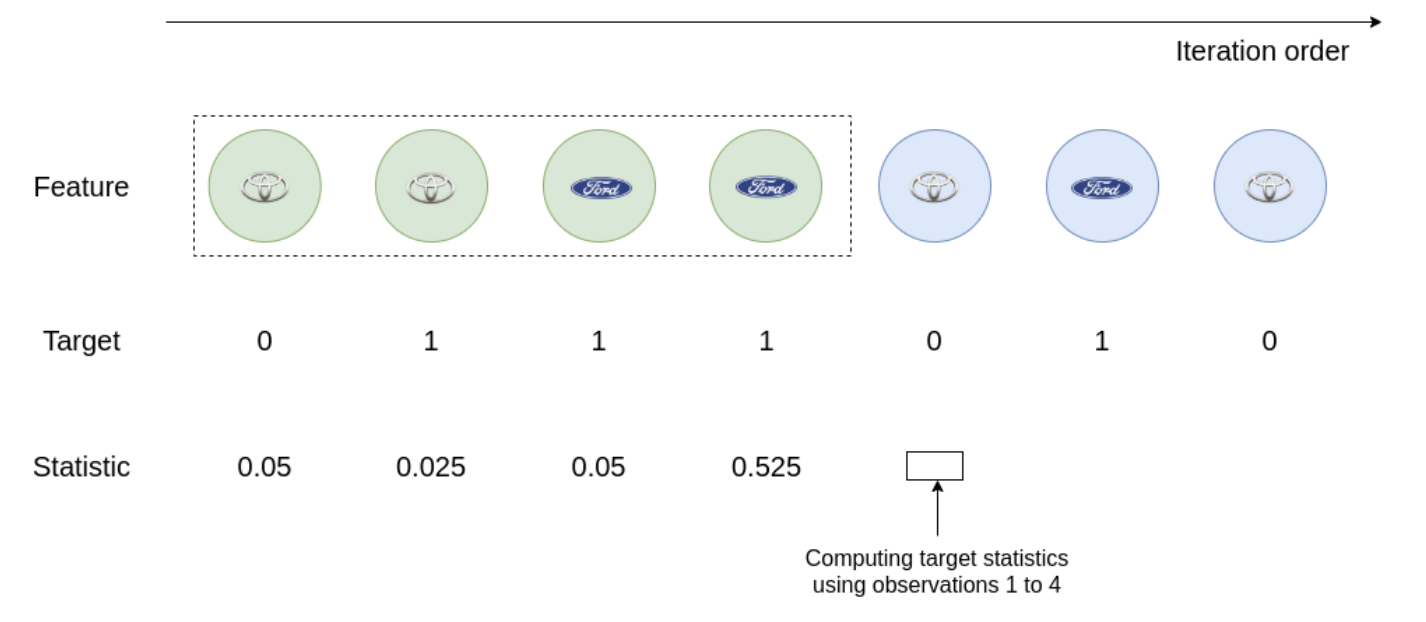
\includegraphics[scale=0.65]{figures/catboost_encoding.png}
	\caption{ Пример кодирования с помощью Catboost }\label{fig:catboost_encoding}
\end{figure}

Для первого элемента в последовательности, изображенной на рис. \pic{fig:catboost_encoding} статистика рассчитывается так (здесь положено $ prior = 0.05 $)
\begin{align*}
	ctr = \dfrac{ 0 + 0.05 }{ 0 + 1} = 0.05.
\end{align*}

Для второго элемента
\begin{align*}
	ctr = \dfrac{ 0 + 0.05 }{ 1 + 1 } = 0.025.
\end{align*}

Для пятого элемента
\begin{align*}
	ctr = \dfrac{ 1 + 0.05 }{ 2 + 1} = 0.35.
\end{align*}

Первые наблюдения не содержат достаточного количества обучающих экземпляров для получения надежных оценок, поэтому авторы Catboost предложили использовать несколько случайных перестановок (для каждой перестановки создается своя кодировка), а затем усреднить кодировки по числу перестановок.

\section{Кодирование категориальных переменных с помощью Байесовского целевого кодирования}

Техника Байесовского целевого кодирования (Bayesian Target Encoding) \url{https://mattmotoki.github.io/beta-target-encoding.html} -- это техника проектирования признаков, используемая для отображения категориальных переменных на числовые.

Преимущества использования техники Байесовского целевого кодирования:
\begin{itemize}
	\item  гиперпараметры легко интерпретировать,
	
	\item приемы оценки гиперпараметров подходят для динамического обучения,
	
	\item легко обобщить технику на статистики отличные от среднего,
	
	\item легко выбрать распределение для зашумления переменной.
\end{itemize}

\section{Приемы работы с библиотекой для анализа временных рядов Darts}

\subsection{Общие сведения}

Darts поддерживает работу с большими наборами данных, которые не помещаются в оперативную память. Для этого вместо метода \texttt{fit()} следует использовать метод \texttt{fit\_from\_dataset()}, что позволит организовать процедуру отложенных вычислений. Можно реализовать свой собственный набор данных, создав подкласс \texttt{TrainingDataset}.

\subsection{Модели на пакете временных рядов}

Библиотека \texttt{darts} представляет собой Python-библиотеку для прогнозирования на временных рядах. Включает различные модели: от классических ARIMA до моделей на базе глубоких нейронных сетей. Некоторые модели могут работать с многомерными временными рядами.

\texttt{Darts} включает множество моделей, но не все из них поддерживают обучение на многомерных временных рядах. Модели, которые поддерживают обучение на многомерных временных рядах назыавют \emph{глобальными моделями}. На текущий момент в \texttt{darts} реализовано 4 глобальные модели:
\begin{itemize}
	\item RNN,
	
	\item Temporal Convolutional Networks (TCN),
	
	\item N-Beats,
	
	\item Transformer.
\end{itemize} 

Различают \emph{целевые временные ряды} (target time series), по которым мы собираемся строить прогноз, и \emph{вспомогательные временные ряды} (covariate time series), которые могут быть полезны при прогнозировании целевого временного ряда. Вспомогательные временные ряды еще называют внешними данными.

Все глобальные модели, перечисленные выше, поддерживают обучение по нескольким временным рядам. Кроме того, все они (кроме N-Beats) имеют \emph{многомерную} и \emph{ковариационную поддержку}.

Многомерная поддрежка означает, что модель может обучаться на многомерных временных рядах (т.е. временных рядах, которые имеют более одного измерения). Целевой временной ряд может иметь одно (как это часто бывает) или несколько измерений. Временной ряд с несколькими измерениями на самом деле является обычным временным рядом, где значения в каждой временной метке ассоциированы с векторами, а не скалярами.

Ковариационная поддержка означает, что можно использовать вспомогательные временных ряды (внешние данные).

Перечисленные модели содержат нейронную сеть, которая получает фрагменты временного ряда и возвращает прогноз. Фактическая внутренняя модель нейронной сети создается только во время обучения.

Для управления поведением модели используется два параметра: \texttt{input\_chunk\_length} -- ширина окна -- и \texttt{output\_chunk\_length} -- <<длина>> выходных данных (прогноза), создаваемых моделью. 

Пример с одномерным временным рядом. Будем использовать N-BEATS с окном в 24 точки (\texttt{input\_chunk\_length=24}) и прогнозом на следующие 12 точек (\texttt{output\_chunk\_length=12}). То есть модель строит прогноз на год, опираясь на последнием 2 года.

\begin{lstlisting}[
style = ironpython,
numbers = none	
]
# fix python path if working locally
from utils import fix_pythonpath_if_working_locally
fix_pythonpath_if_working_locally()

import pandas as pd
import numpy as np
import torch
import matplotlib.pyplot as plt

from darts import TimeSeries
from darts.utils.timeseries_generation import gaussian_timeseries, linear_timeseries, sine_timeseries
from darts.models import RNNModel, TCNModel, TransformerModel, NBEATSModel
from darts.metrics import mape, smape
from darts.dataprocessing.transformers import Scaler
from darts.utils.timeseries_generation import datetime_attribute_timeseries
from darts.datasets import AirPassengersDataset, MonthlyMilkDataset

torch.manual_seed(1); np.random.seed(1)  # for reproducibility

series_air = AirPassengersDataset().load()
series_milk = MonthlyMilkDataset().load()

series_air.plot(label='Number of air passengers')
series_milk.plot(label='Pounds of milk produced per cow')
plt.legend();

scaler_air, scaler_milk = Scaler(), Scaler()
series_air_scaled = scaler_air.fit_transform(series_air)
series_milk_scaled = scaler_milk.fit_transform(series_milk)

series_air_scaled.plot(label='air')
series_milk_scaled.plot(label='milk')
plt.legend();

train_air, val_air = series_air_scaled[:-36], series_air_scaled[-36:]
train_milk, val_milk = series_milk_scaled[:-36], series_milk_scaled[-36:]

model_air = NBEATSModel(input_chunk_length=24, output_chunk_length=12, n_epochs=200, random_state=0)

model_air.fit(train_air, verbose=True) # Traning loss: 0.0002

# Прогноз строится на 36 точек, а параметр output_chunk_length=12. Но это не проблема. Просто внутренняя модель будет вызываться несколько раз на своих собственных выходах. То есть в данном случае внутренняя модель будет вызвана 3 раза
pred = model_air.predict(n=36)

series_air_scaled.plot(label='actual')
pred.plot(label='forecast')
plt.legend();
print('MAPE = {:.2f}%'.format(mape(series_air_scaled, pred)))
\end{lstlisting}

\begin{figure}[h]
	\centering
	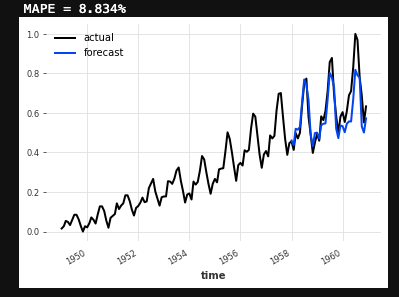
\includegraphics[scale=0.65]{figures/darts_nbeats_air_pred.png}
	\caption{ Пример использования N-BEATS для прогноза }\label{fig:darts_nbeats_air_pred}
\end{figure}

Пример обучения модели на нескольких временных рядах.
\begin{lstlisting}[
style = ironpython,
numbers = none	
]
model_air_milk = NBEATSModel(input_chunk_length=24, output_chunk_length=12, n_epochs=100, random_state=0)
model_air_milk.fit([train_air, train_milk], verbose=True)
\end{lstlisting}

Здесь при обучении использовались два временных ряда, поэтому при построении прогноза следует указать какой временной нужно рассмтривать как целевой, а какой -- как вспомогательный.

\begin{lstlisting}[
style = ironpython,
numbers = none	
]
pred = model_air_milk.predict(
    n=36,
    series=train_air # здесь указывается имя временного ряда,
                                     # для которого следует строить прогноз
)
\end{lstlisting}

Пример обучения модели с учетом вспомогательных многомерных временных рядов
\begin{lstlisting}[
style = ironpython,
numbers = none
]
model_cov = RNNModel(
    input_chunk=24,
    training_length=32,
    n_epochs=300,
    random_state=0
)

model_cov.fit(
    series=[train_air, train_milk],
    covariates=[air_train_covariates, milk_train_covariates],
    verbose=True
)

pred_cov = model_cov.predict(
    n=12,
    series=train_air, # имя переменной, связанной с временным рядом, для которого следует построить прогноз
    covariates=air_covariates # передается вся информация о многомерных вспомогательных временных рядах
)
series_air_scaled.plot(label="actual")
pred_cov.plot(label="forecast")
plt.legend()
\end{lstlisting}

ЗАМЕЧАНИЕ: преобразовать временной ряд в обычный NumPy-массив можно с помощью метода \texttt{.values()}
\begin{lstlisting}[
style = ironpython,
numbers = none	
]
time_series.values().ravel() # 1D numpy-array
\end{lstlisting}

\subsection{Рекуррентные нейронные сети}

Darts включает две модели на базе рекуррентных нейронных сетей: \texttt{RNNModel} и \texttt{BlockRNNModel}. Модель \texttt{RNNModel} полностью рекуррентна. Эта модель подходит для тех случаев, когда целевой временной ряд сильно зависит от вспомогательного.

Модель \texttt{BlockRNNModel} имеет рекуррентный этап кодирования входов и этап декодирования полносвязной нейронной сети, который строит прогноз длины \texttt{output\_chunk\_length} на основе последних скрытых состояний этапа декодирования.

Пример
\begin{lstlisting}[
style = ironpython,
numbers = none	
]
import torch
import torch.nn as nn
import torch.optim as optim
import numpy as np
import pandas as pd
import shutil
from sklearn.preprocessing import MinMaxScaler
from tqdm import tqdm_notebook as tqdm

from torch.utils.tensorboard import SummaryWriter
import matplotlib.pyplot as plt

from darts import TimeSeries
from darts.dataprocessing.transformers import Scaler
from darts.models import RNNModel, ExponentialSmoothing, BlockRNNModel
from darts.metrics import mape
from darts.utils.statistics import check_seasonality, plot_acf
from darts.datasets import AirPassengersDataset, SunspotsDataset
from darts.utils.timeseries_generation import datetime_attribute_timeseries

series = AirPassengersDataset().load()

train, val = series.split_after(pd.Timestamp("1959-01-01"))
transformer = Scaler()
train_transformed = transformer.fit_transform(train)
val_transformed = transformer.transform(val)
series_transformed = transformer.transform(series)

year_series = datetime_attribute_timeseries(
    pd.date_range( 
        start=series.start_time(),
        freq=series.freq_str,
        periods=1000
    ),
    attribute="year",
    one_hot=False
)

year_series = Scaler().fit_transform(year_series)
month_series = datetime_attribute_timeseries(year_series, attribute="month", one_hot=True)
covariates = year_series.stack(month_series)
cov_train, cov_val = covariates.split_after(pd.Timestamp("1959-01-01"))

rnnmodel = RNNModel(
    model = "LSTM",
    hidden_dim=20,
    dropout=0,
    batch_size=16,
    n_epochs=300,
    optimizer_kwargs={"lr" : 1e-3},
    model_name = "AIR_RNN",
    log_tensorboard = True,
    random_state = 42,
    training_length=20,
    input_chunk_length=14,
    force_reset=True,
)

rnnmodel.fit(
    train_transformed, # целевой временной ряд
    covariates=cov_train, # обучающий поднабор вспомогательного многомерного временного ряда
    val_series=val_transformed, # тестовый поднабор целевого временного ряда
    val_covariates=cov_val, # тестовый поднабор вспомогательного многомерного временного ряда
    verbose=True
)

def eval_model(model):
    pred_series = rnnmodel.predict(n=26, covariates=covariates)
    series_transformed.plot(label="actual")
    pred_series.plot(label="forecast")
    plt.title(f"MAPE: {mape(pred_series, val_transformed):.2f}")

eval_model(rnnmodel)

best_model = RNNModel.load_from_checkpoint(model_name="AIR_RNN", best=True)
\end{lstlisting}

\section{Приемы работы с библиотекой для анализа временных рядов sktime}

Библиотека \texttt{sktime} \url{https://www.sktime.org/en/latest/} предназначена для задач классификации, регрессии, кластеризации и прогнозирования на временных рядах.

Извлечение признаков из временного ряда с использованием библиотеки \texttt{sktime} и подбор гиперпараметров с \texttt{skopt.BayesSearchCV}
\begin{lstlisting}[
style = ironpython,
numbers = none	
]
from sktime.transformations.panel.tsfresh import TSFreshFeatureExtractor
from sklearn.pipeline import make_pipeline
from sklearn.model_selection import StratifiedKFold
from skopt import BayesSearchCV
from skopt.plots import plot_objective
from collections import OrderedDict

...
X_train, X_test, y_train, y_test = train_test_split(X, y)

pipe = make_pipeline(
    TSFreshFeatureExtractor(
        default_fc_parameters="minimal",
        show_warnings=False
    ),
    MinMaxScaler(),
    GradientBoostingClassifier()
).fit(X_train, y_train)

pipe.get_params()

params = {
	"gradientboostingclassifier__learning_rate" : Real(0.5, 1.0, prior="uniform"),
	"gradientboostingclassifier__max_features" : Real(0.9, 1.0, prior="uniform"),
	"gradientboostingclassifier__max_depth" : Integer(5, 10),
}

opt = BayesSearchCV(
    estimator=pipe,
    search_spaces=params,
    cv=StratifiedKFold(n_splits=3, shuffle=True),
    n_iter=50,
)

opt.fit(X_train, y_train)

opt.best_params_

dimensions = [key.replace("gradientboostingclassifier__", "") for key in opt.best_params_.keys()]

plot_objective(
    opt.optimizer_results_[0],
    dimensions=dimensions,
    size=3.5,
    levels=10
);
\end{lstlisting}



\section{Приемы работы с открытой Amazon-библиотекой для анализа временных рядов GluonTS}

В июне 2019 Amazon выложила в открытый доступ библиотеку GluonTS \url{https://github.com/awslabs/gluon-ts}, позволяющую максимально быстро и эффективно строить, оценивать и использовать модели временных рядов, основанные на глубоком обучении и вероятностном подходе.

До этого момента один из самых открытых библиотек для работы с временными рядами был \texttt{Prophet}. В отличие от GluonTS, Prophet использует более простой метод -- аддитивную нелинейную модель временного ряда. Prophet плохо работает на данных без ярко выраженной сезонности!

GluonTS использует рекуррентные нейронные сети, свертки и механизмы внимания. В частности, GluonTS содержит:
\begin{itemize}
	\item инструменты, необходимые для построения и обучения наиболее распростаненных архитектур нейронных сетей, а также компоненты для моделирования и трансформации вероятностных распределений;
	
	\item механизмы для загрузки и предварительной обработки данных, в том числе автоматической генерации признаков из временных рядов;
	
	\item несколько готовых к использованию state-of-the-art прогностических моделей;
	
	\item инструменты для оценки и сравнения различных моделей.
\end{itemize}

GluonTS возвращает не точечный прогноз, а вероятностное распределение. Таким образом, можно с легкостью оперировать доверительными интервалами прогноза и с любой наперед заданной вероятностью получать диапазон наиболее вероятных будущих значений ряда.

Установить GluonTS можно так
\begin{lstlisting}[
style = bash,
numbers = none
]
pip install -U mxnet~=1.7 gluonts
\end{lstlisting}

Рассмотрим пример с использованием глубокой авторегрессионной моделью \href{https://arxiv.org/abs/1704.04110}{DeepAR}
\begin{lstlisting}[
style = ironpython,
numbers = none
]
from gluonts.model.deepar import DeepAREstimator
from gluonts.mx.trainer import Trainer

estimator = DeepAREstimator(
    freq="D",
    prediction_length=30,
    trainer=Trainer(epochs=20)
)

predictor = estimator.train(training_data=training_data)
\end{lstlisting}




\section{Приемы работы с библиотекой tsfresh для автоматического проектирования признаков на временных рядах}

\subsection{Формат данных}

Функция извлечения признаков \texttt{extract\_features} принимает на вход объект \texttt{pandas.DataFrame}. Рассмотрим четыре наиболее важных параметра этой функции:
\begin{itemize}
	\item \texttt{column\_id}: задает индентификационный номер экзепмляра. Признаки рассчитываются индивидуально для каждого экземпляра (то есть для каждого уникального идентификационного номера). Результирующая матрица признаков будет содержать по одной строке на каждый идентификационный номер. Например, каждый робот это отдельный экземпляр, поэтому у каждого робота свой идентификационный номер.
	
	\item \texttt{column\_sort}: здесь указывается имя столбца, по которому можно сортировать временной ряд (например, временные метки). Если опустить этот параметр, то будет предполагаться, что столбец уже отсортирован по возрастанию.
	
	\item \texttt{column\_value}: здесь указывается столбец, который содержит фактические значения временных рядов. Это, например, могут быть измерения датчиков.
	
	\item \texttt{column\_kind}: здесь указываются имена типов временных рядов.
\end{itemize}

ЗАМЕЧАНИЕ: ни один из этих параметров не может содержать \texttt{NaN}, \texttt{Inf} или \texttt{-Inf}.

Вот перечень различных форматов входных данных:
\begin{itemize}
	\item плоский формат DataFrame,
	
	\item пакетный формат DataFrame,
	
	\item словарь плоских DataFrame.
\end{itemize}

Разница между плоским и пакетным форматом заключается в том, что в случае пакетного формата требуется указывать параметры \texttt{column\_value} и \texttt{column\_kind}, а в случае плоского формата нет.

Если параметрам \texttt{column\_value} и \texttt{column\_kind} передано значение \texttt{None}, то предполагается, что временной ряд находится в \emph{плоском} формате. Это означает, что каждый отдельный временной ряд должен быть представлен отдельным столбцом.

Например, если ведется наблюдение за двумя объектами A и B и фиксируются какие-то измерения в моменты времены $ t_1, t_2, t_3 $, то набор данных будет выглядеть, как показано на \pic{fig:flat_df_ts}.

\begin{figure}[h]
	\centering
	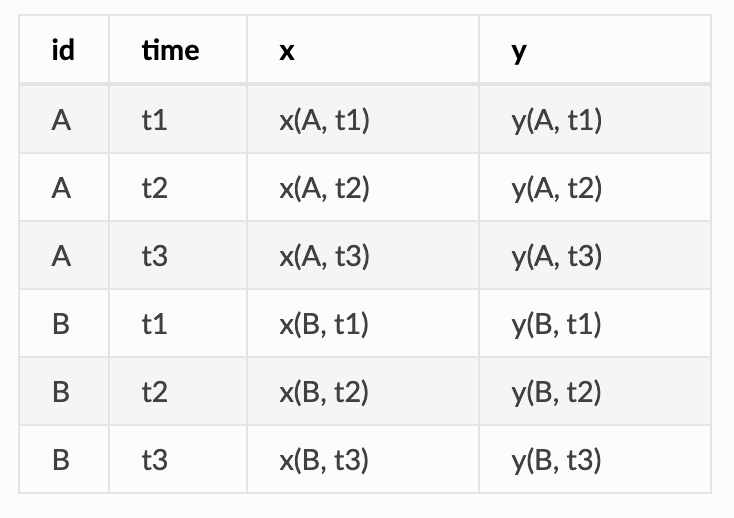
\includegraphics[scale=0.25]{figures/flat_df_ts.png}
	\caption{ Временные ряды, представленные в плоском формате }\label{fig:flat_df_ts}
\end{figure}

\begin{lstlisting}[
style = ironpython,
numbers = none
]
...
extract_features(
    column_id="id",
    column_sort="time",
    column_value=None,
    column_kind=None
)
\end{lstlisting}

Если параметры \texttt{column\_value} и \texttt{column\_kind} заданы, то предполагается, что временной ряд имеет \emph{пакетный} (или длинный) формат. Это значит, что разные типы временных рядов располагаются в одном и том же столбце (см. \pic{fig:stack_df_ts}).

\begin{lstlisting}[
style = ironpython,
numbers = none	
]
...
extract_features(
    column_id="id",
    column_sort="time",
    column_kind="kind",
    column_value="value"
)
\end{lstlisting}

\begin{figure}[h]
	\centering
	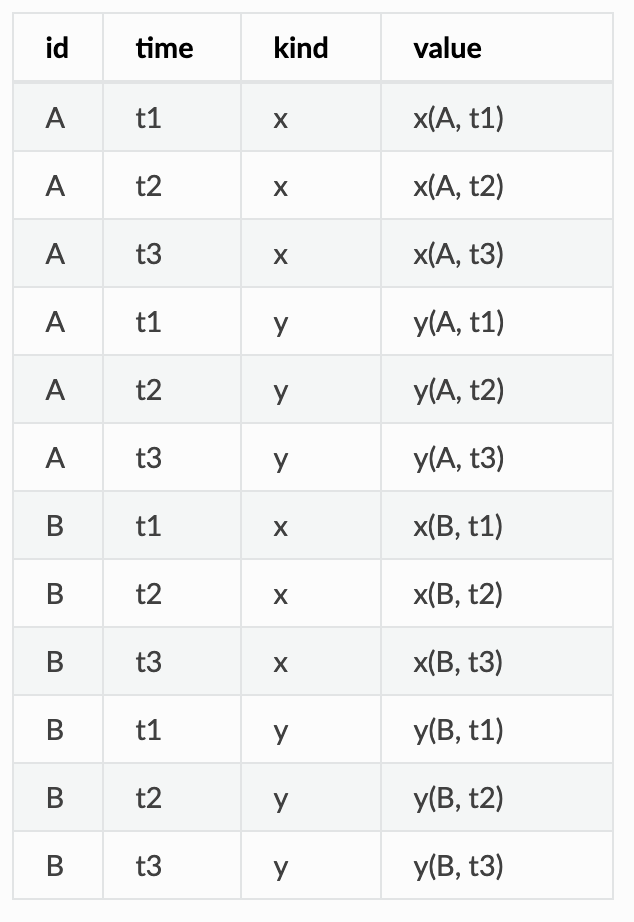
\includegraphics[scale=0.25]{figures/stack_df_ts.png}
	\caption{ Временные ряды, представленные в пакетном формате }\label{fig:stack_df_ts}
\end{figure}

Еще можно разбить набор данных по столбцу \texttt{kind} и тогда временной ряд будет в формате словаря плоских DataFrame (см. \pic{fig:dict_flat_df_ts}).

\begin{lstlisting}[
style = ironpython,
numbers = none	
]
extract_featuers(
    column_id="id",
    column_sort="time",
    column_kind=None,
    column_value="value"
)
\end{lstlisting}

\begin{figure}[h]
	\centering
	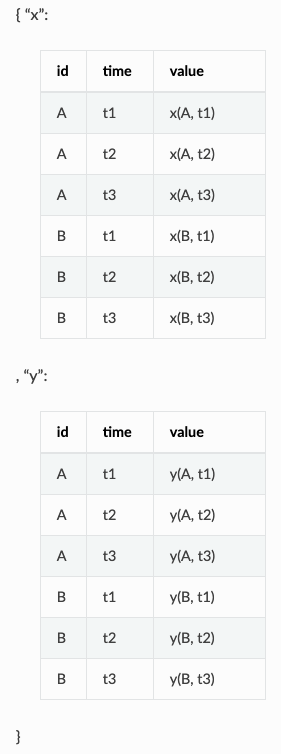
\includegraphics[scale=0.55]{figures/dict_flat_df_ts.png}
	\caption{ Временные ряды, представленные в формате плоских DataFrame }\label{fig:dict_flat_df_ts}
\end{figure}

На выходе всегда будет получать объект DataFrame, представленного на рис. \pic{fig:output_ts}. Такой формат данных ожидает получить на вход функция отбора признаков \texttt{tsfresh.select\_features()}.

\begin{figure}[h]
	\centering
	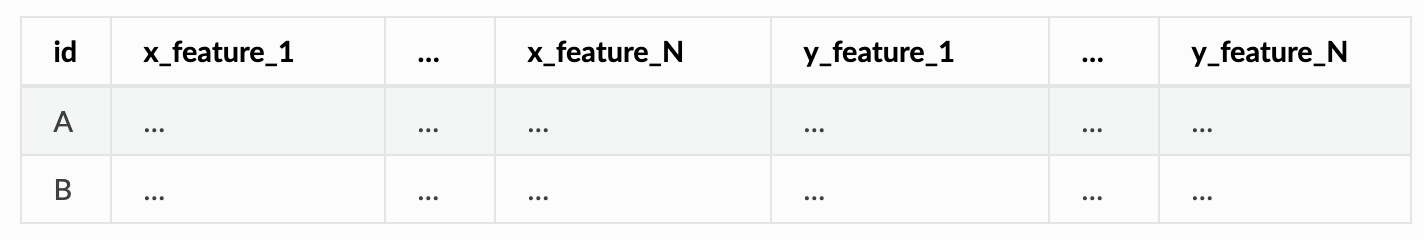
\includegraphics[scale=0.25]{figures/output_ts.png}
	\caption{ Матрица сгенерированных признаков. Выходной формат }\label{fig:output_ts}
\end{figure}




\subsection{Отбор признаков}

Общая проблема отбора признаков заключается в идентификации всех сильно и слабо релевантных атрибутов. Эту проблему особенно сложно решить для классификации и регрессии временных рядов в промышленных приложениях, таких как предиктивное обслуживание или оптимизация производственных линий, для которых каждое значение целевого вектора связано с несколькими временными рядами.

Для того чтобы ограничить число нерелевантных признаков, tsfresh использует FeatuRe Extraction based on Scalabel Hypothesis test.

Алгоритм вызывается с помощью

\texttt{tsfresh.feature\_selection.relevance.calculate\_relevance\_table()}.

Это эффективный алгоритм, масштабируемый алгоритм извлечения признаков, который отбирает доступные признаки на раннем этапе конвейера машинного обучения для задач классификации или регрессии. При этом контролируется ожидаемый процент отобранных, но не имеющих отношения к делу.

Чтобы воспользоваться функцией \texttt{calculate\_relevance\_table} нужно просто передать набор данных в формате \texttt{pd.DataFrame} и целевой вектор в формате \texttt{pd.Series}.

Процесс отбора признаков состоит из  трех этапов (\pic{fig:tsfresh_feature_filter}):
\begin{itemize}
	\item на первом этапе с помощью функции \texttt{tsfresh.feature\_extraction.feature\_calculators} вычисляются признаки, например
\begin{lstlisting}[
style = ironpython,
numbers = none	
]
from tsfresh.feature_extraction import feature_calculators

feature_calculators.abs_energy(X.iloc[0, :]) # 5152503.753728688
feature_calculators.variation_coefficient(X.iloc[0, :]) # 3.3398199304406013
\end{lstlisting}
	
	\item на втором этапе каждый признак \emph{индивидуально} и \emph{независимо} оценивается с точки зрения его значимости для прогнозируемой цели.
	
	Эти тесты содержаться в подмодуле \texttt{tsfresh.feature\_selection.significance\_tests}.
	
	Результатом тестов является вектор p-value, количественно определяющий значимость каждого признака для прогнозируемой переменной
\begin{lstlisting}[
style = ironpython,
numbers = none
]
# низкое значение p-value свидетельствует о высокой важности признака!!!
from tsfresh.feature_selection import significance_tests
significance_tests.target_binary_feature_real_test(X.iloc[:, 0], y, "mann") # 2.6929427727965647e-68
significance_tests.target_binary_feature_real_test(X.iloc[:, 9], y, "mann") # 0.537185602135624
\end{lstlisting}

    \item на третьем этапе вектор p-value оценивается на основе процедуры Бенджамини-Екутиели, чтобы решить какие признаки оставить (процедура заимствована из пакета \texttt{statsmodel}).
\end{itemize}

\begin{figure}[h]
	\centering
	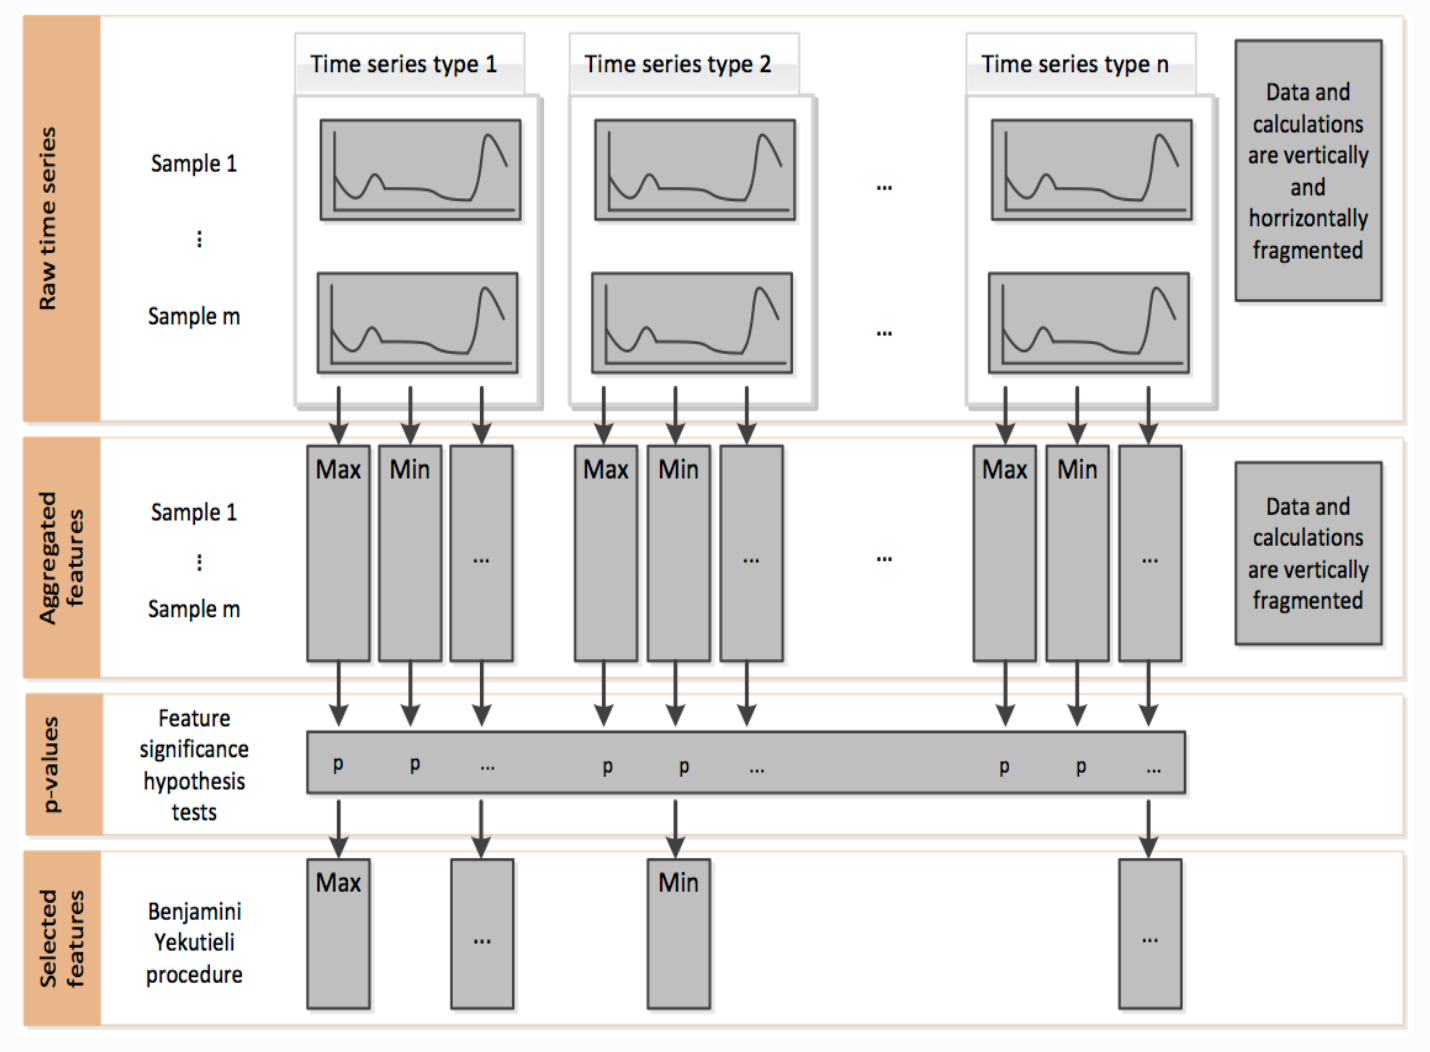
\includegraphics[scale=0.35]{figures/tsfresh_feature_filter.png}
	\caption{ Процедура отбора признаков с помощью tsfresh }\label{fig:tsfresh_feature_filter}
\end{figure}

\subsection{Извлечение признаков}

Когда данные одномерного временного ряда приведены к нужному для tsfresh формату (например, к длинному формату), можно к этому набору данных применить функцию \texttt{tsfresh.utilities.dataframe\_functions.roll\_time\_series()}. У этой функции есть два основные параметра:
\begin{itemize}
	\item \texttt{max\_timeshift}: если передано значение отличное от \texttt{None}, то окно будет иметь максимальную ширину равную \texttt{max\_timeshift}. В противном случае (т.е. когда \texttt{max\_timeshift=None}) ширина окна будет увеличиваться до бесконечности.
	
	\item \texttt{min\_timeshift}: все извлеченные временные ряды, имеющие длину меньшую или равную \texttt{min\_timeshift} будут исключены из результатов.
\end{itemize}

Новый набор данных \texttt{df\_rolled} состоять из старого набора данных плюс новый столбец \texttt{id}. Например
\begin{lstlisting}[
style = ironpython,
numbers = none	
]
# df
#	id	            time	      value
# 0	0	2020-01-31	-0.349435
# 1	0	2020-02-29	-1.933673
# 2	0	2020-03-31	

from tsfresh.utilities.dataframe_functions import roll_time_series
df_rolled = roll_time_series(
	df,
	column_id="id",
	column_sort="time"
)

df_rolled.sort_values(by="id")
# id	             time	       value
# 2	(0, 2020-01-31 00:00:00)	2020-01-31	-0.349435 Группа 1
# ----------------------------------------------
# 0	(0, 2020-02-29 00:00:00)	2020-01-31	-0.349435 Группа 2
# 1	(0, 2020-02-29 00:00:00)	2020-02-29	-1.933673
# ----------------------------------------------
# 3	(0, 2020-03-31 00:00:00)	2020-01-31	-0.349435 Группа 3
# 4	(0, 2020-03-31 00:00:00)	2020-02-29	-1.933673
# 5	(0, 2020-03-31 00:00:00)	2020-03-31	-1.910476

# Группы можно посмотреть так
df_rolled.groupby("id").groups # {(0, 2020-01-31 00:00:00): [2], (0, 2020-02-29 00:00:00): [0, 1], (0, 2020-03-31 00:00:00): [3, 4, 5]}

# Номера групп 
df_rolled.groupby("id").ngroup()
# 0
# 1
# 1
# 2
# 2
# 2
\end{lstlisting}

ЗАМЕЧАНИЕ: Вторым элементом мультииндекса будет <<старшая>> временная метка диапазона.

Теперь можно применить функцию \texttt{extract\_features} для извлечения признаков
\begin{lstlisting}[
style = ironpython,
numbers = none	
]
from tsfresh.feature_extraction import settings
from tsfresh.utilities.dataframe_functions import impute

df_features = extract_features(
    df_rolled,
    column_id="id",
    column_sort="time",
    impute_function=impute,
    default_fc_parameters=settings.MinimalFCParameters()
)
\end{lstlisting}

На выходе будет получена матрица признаков со сгенерированным вектором признаков для каждой уникальной комбинации мультииндекса (то есть для каждой группы-окна)
\begin{lstlisting}[
style = ironpython,
numbers = none	
]
	                       value__sum_values	value__median	value__mean	value__length	value__standard_deviation	value__variance	
0	2020-01-31	-0.349435	-0.349435	-0.349435	1.0	0.000000	0.000000
     2020-02-29	-2.283108	-1.141554	-1.141554	2.0	0.792119	0.627453
     2020-03-31	-4.193584	-1.910476	-1.397861	3.0	0.741410	0.549689
\end{lstlisting}

ОЧЕНЬ ВАЖНО: признаки вычисляются для каждой группы-окна, сгруппированной по мультииндексу: сначала вычисляются средняя, медиана, дисперсия и пр. по первой группе, состоящей из одного элемента, затем эти же признаки -- для второй группы, состоящей из двух элементов, затем эти же признаки -- для третьей группы, состоящей из трех элементов и т.д. Например, как видно из результирующей матрицы признаков, значение -2.283108 получено как сумма по элементам второй группы (т.е. по второму окну), а значение 0.549689, как дисперсия по трем элементам (т.е. по третьему окну) и так далее
\begin{lstlisting}[
style = ironpython,
numbers = none	
]
fake_df.loc[0, "value"] + fake_df.loc[1, "value"] # value_sum_values = -2.283108
np.array([
    fake_df.loc[0, "value"],
    fake_df.loc[1, "value"],
    fake_df.loc[2, "value"]
]).std() ** 2  # value_variance = 0.549689
\end{lstlisting}

Если в функции \texttt{roll\_time\_series()} параметру \texttt{min\_timeshift} передать значение 1, то группы-окна, состоящие из одного элемента будут исключены из результирующей матрицы признаков (как малоинформативные).

Шаблон отображения ординат временного ряда на векторы признаков:
\begin{itemize}
	\item Приводим временной ряд к нужному формату данных (например, к пакетному-длинному),
	
	\item Применяем функцию \texttt{roll\_time\_series()} для того чтобы сформировать группы-окна, состоящие из одного элемента, двух элементов и т.д. Вычисленное значение признака привязывается к крайней правой временной метке рассматриваемой группы-окну.
	
	\item Применяем функцию \texttt{extract\_features()} чтобы для каждой временной метки получить вектор признаков. Если задать \texttt{min\_timeshift}, то можно из результирующей матрицы признаков исключить группы заданного размера. А если задать \texttt{max\_timeshift}, то можно скользить по временному ряду окном (а не расширять исходное окно до бесконечности, начиная с первых элементов временного ряда). Группа-окно временного ряда будет включать \texttt{max\_timeshift + 1} элементов.
\end{itemize}

В итоге получается, что в общем случае каждой временной метке временного ряда отвечает вектор сгенерированных признаков. И таким образом мы приходим к обычной базовой аналитической таблице.

ОЧЕНЬ ВАЖНО: если экземпляр представляет собой временной ряд, то вектор признаков вычисляется по всем ординатам этого временного ряда. Другими словами, временной ряд отображается на вектор сгенерированных признаков.




\subsection{Загрузка больших наборов данных}

Для загрузки данных из формата parquet
\begin{lstlisting}[
style = ironpython,
numbers = none	
]
import dask.dataframe as dd
from tsfresh import extract_features

df = dd.read_parquet(...)

X = extract_features(
    df,
    column_id="id",
    column_sort="time",
    pivot=False
)

res = X.compute()
\end{lstlisting}

\subsection{Загрузка фрагментов данных с поддрежкой joblib}

Если требуется загрузить фрагмент набора данных и для него посчитать признаки, то можно воспользоваться библиотекой \texttt{joblib}
\begin{lstlisting}[
style = ironpython,
numbers = none	
]
from pathlib2 import Path, PosixPath, WindowsPath
from typing import Union

def features_generator(
    path_fo_file: Union[PosixPath, WindowsPath]
) -> pd.DataFrame:
    """
    Возвращает одну строку сгенерированных признаков в формате pd.DataFrame
    """
    signals = pd.read_csv(path_to_file)
    sed_id = path_fo_file.name.split(".")[0]
    
    extracted_features = extract_features(
        signals,
        column_id = "segment_id",
        default_fc_parameters=EffecientFCParameters(),
        impute_function = impute,
        n_jobs = 0,
        desable_progressbar = False,
        chunksize = None
    )
    
    return extracted_features
    

# delayed принимает каррировано функцию и ее аргумент
rows = Parallel(n_jobs=-1)(
    delayed(features_generator)(segment) for segment in train_files_list
)

train_set = pd.concat(rows, axis=0)
\end{lstlisting}



\subsection{Общий порядок работы}



При работе с временными рядами могут возникнуть две ситуации:
\begin{itemize}
	\item Требуется построить прогноз, основываясь на предыдущих значениях временного ряда,
	
	\item Требуется использовать временной ряд как признак экземпляра.
\end{itemize}

Основная идея библиотеки \texttt{tsfresh} -- сгенерировать как можно больше признаков (если позволяют вычислительные ресурсы), а затем при помощи моделей или статистических критериев из этих признаков уже можно отобрать только те, которые релевантны задаче. Безусловно, не все признаки окажутся полезными.

Рассмотрим прмер распознавания активности человека по данным акселерометра
\begin{lstlisting}[
style = ironpython,
numbers = none	
]
from tsfresh.examples.har_dataset import download_har_dataset, load_har_dataset, load_har_classes
from tsfresh import extract_features, extract_relevant_features, select_features
from tsfresh.utilities.dataframe_functions import impute
from tsfresh.feature_extraction import settings

from sklearn.tree import DecisionTreeClassifier
from sklearn.model_selection import train_test_split
from sklearn.metrics import classification_report

import pandas as pd
import numpy as np
\end{lstlisting}

Пусть у нас есть 7352 наблюдения, каждому из которых соответствет 128 показаний акселерометра и одна из шести возможных активностей
\begin{lstlisting}[
style = ironpython,
numbers = none	
]
download_har_dataset()
data = load_har_dataset()
y = load_har_classes()
\end{lstlisting}

То есть эти 128 наблюдений акселерометра можно рассматривать как признаки. Другими словами, каждый экземпляр обучающего набора данных это временной ряд.
\begin{lstlisting}[
style = ironpython,
numbers = none	
]
X_train, X_test, y_train, y_test = train_test_split(data, y, test_size=.2)

cl = DecisionTreeClassifier()
cl.fit(X_train, y_train)
print(classification_report(y_test, cl.predict(X_test)))
\end{lstlisting}

В tsfresh есть различные варианты извлечения признаков, которыми можно воспользоваться из коробки и особенно не думать на счет содержания. Отличаются они лишь количеством рассчитываемых признаков, а значит и скоростью обработки данных. Один из основных наборов признаков это \texttt{TimeBasedFCParameters}. Этот метод посчитает по нашему ряду линейный тренд, возьмет оттуда значение коэффициента R2, intercept, slope, стандартную ошибку и p-value и все это сделаем новыми признаками.

\begin{lstlisting}[
style = ironpython,
numbers = none	
]
settings_time = settings.TimeBasedFCParameters()
settings_time.update(settings_minimal)
\end{lstlisting}

Есть еще \texttt{EfficientFCParameters}, \texttt{Efficient}
\begin{lstlisting}[
style = ironpython,
numbers = none	
]
settings_efficient = settings.EfficientFCParameters()
\end{lstlisting}

Построим новое признаковое пространство. Для начала следует преобразовать набор данных в формат, необходимый для работы библиотеки. В этом формате у нас будет всего два столбца: в первом будут храниться вся наблюдения акселерометров, а во втором -- соответствующий индекс наблюдения.
\begin{lstlisting}[
style = ironpython,
numbers = none	
]
data_long = pd.DataFrame(
    {
        0 : data.values.flatten(), # разворачивает весь набор по строке в одну длинную строку
        # np.arange(5).repeat(3)    # array([0, 0, 0, 1, 1, 1, 2, 2, 2, 3, 3, 3, 4, 4, 4])
        1 : np.arange(data.shape[0]).repeat(data.shape[1])
    }
)
\end{lstlisting}

Извлекаем признаки при помощи \texttt{extract\_features}, указав в качестве параметров для извлечения соответствующий список (\texttt{settings.TimeBasedFCParameters}, \texttt{Efficient} и т.д.).

Также укажем для параметра \texttt{impute\_function} фукнцию \texttt{impute} из \texttt{tsfresh.utilities.dataframe\_functions}. Эта функция автоматически заполнит все пропуски в получившимся наборе данных (если они вдруг там появятся).
\begin{lstlisting}[
style = ironpython,
numbers = none	
]
X = extract_features(
    data_long,
    column_id=1,
    impute_function=impute,
    default_fc_parameters=settings.EfficientFCParameters
)
X.shape # (7352, 788)
\end{lstlisting}

Теперь каждому экземпляру набора данных отвечает не 128 сырых значений акселерометра (ординаты акселерограммы как признаки), а 788 извлеченных признаков.
\begin{lstlisting}[
style = ironpython,
numbers = none	
]
X_train, X_test, y_train, y_test = train_test_split(X, y, test_size=0.2)
cl = DecisionTreeClassifier()
cl.fit(X_train, y_train)
\end{lstlisting}

Но скорее всего, многие из извлеченных признаков на самом деле не нужны для построения предсказаний и могут быть спокойно исключены. Для этого в библиотеке есть метод \texttt{select\_features}, который рассчитывает важность текущего признака для предсказания класса. После расчета ненужные признаки отбрасываются по p-value, при этом в функцию зашита поправка Бенджамини-Иекутиели на множественное тестирование.

ЗАМЕЧАНИЕ: \texttt{select\_features} работает только с бинарной классификацией!

\begin{lstlisting}[
style = ironpython,
numbers = none
]
relevant_features = set()

for label in y.unique():
    y_train_binary = y_train == label
    X_train_filtered = select_features(X_train, y_train_binary)
    relevant_features = relevant_features.union(set(X_train_filtered.columns))
    
len(relevant_features) # 352
\end{lstlisting}

В результате получили более компактное пространство признаков.

\section{Разбор Kaggle соревнования Volcanic Eruption Prediction Competition}

Ссылка на соревнование \url{https://www.kaggle.com/c/predict-volcanic-eruptions-ingv-oe/data}. Здесь требуется опираясь на пакет временных рядов (10 временных), разбитых на сегменты, научиться прогнозировать времея до следующего извержения.

Видимо данные подготавливались следующим образом. На пакете временных рядов отмечались моменты времени, в которые происходило извержение. Время до извержения, видимо, разыгрывалось с помощью равномерного распределения. То есть генератор псевдослучайных равномерно распределенных чисел возвращает некоторое значение, на которое мы отступаем в прошлое от момента времени, соответствующего извержению вулкана. А затем от полученной временной метки (время до извержения) отступаем в прошлое на 10 минут. Таким образом, пакет из 10 временных рядов разбивается на сегменты, которым ставится в соответствие время до извержения. Под обучения отводится 4431 сегмент, а под тест 4520 сегментов. Каждый сегмент имеет 60000 ординат (10 минут записи сенсора).

Чтобы расположить несколько временных рядов все вместе, то можно использовать \texttt{subplots=True}
\begin{lstlisting}[
style = ironpython,
numbers = none	
]
df_1000015382.iloc[:right_border, :].plot(
    figsize=(15, 8),
    subplots=True, # <- NB
)
plt.legend()
\end{lstlisting}

ЗАМЕЧАНИЕ: анализ матрицы признаков на коллинеарность (то есть на линейную зависимость между признаками) можно провести с помощью \emph{матрицы Грама}. Матрица Грама это квадратная симметрическая матрица, элементы которой представляют собой скалярные произведения признаков (вектор-столбцов)
\begin{align*}
	\underset{n \times n}{G}  = \Big( \lbrace v_i, v_j \rbrace \Big)_{i, j=1}^n
\end{align*}

Если в матрице признакового описания объекта есть \emph{коллинеарные} признаки (линейно-зависимые), то определитель матрицы Грама (\emph{грамиан}) будет равен нулю, в противном случае будет отличен от нуля. Дело в том, что коллинеарные признаки образуют линейно-зависимую подсистему, а система, содержащая линейно-зависимую подсистему сама линейно-зависима, а определитель матрицы Грама (как и определитель любой другой матрицы) на линейно-зависимой системе обращается в нуль.

Ванильная реализация для вычисления грамиана
\begin{lstlisting}[
style = ironpython,
numbers = none	
]
def compute_Gramian(data: pd.DataFrame) -> np.float64:
    """Вычисляет грамиан"""
    gram_matrix = []

    features_n = data.shape[1]
    for feature_idx_i in range(features_n):
        for feature_idx_j in range(features_n):
            gram_matrix.append(
                data.values[:, feature_idx_i] @ data.values[:, feature_idx_j]
            )

    gram_matrix_arr = np.array(gram_matrix).reshape(features_n, features_n)

    return np.linalg.det(gram_matrix_arr)
    
compute_Gramian(boston_df) # 1.3188062420717119e+53
compute_Gramian(boston_df_colinear) # 0.0 <- значит есть ЛИНЕЙНО-ЗАВИСИМЫЕ признаки
\end{lstlisting}

ЗАМЕЧАНИЕ: для того чтобы Pandas мог читать большой файл прямо в оперативную память следует добавить в вызов фукнций чтения (\texttt{pd.read\_csv}, \texttt{pd.read\_parquet} и т.д.) флаг \texttt{memory\_map=True}. В этом случае можно повысить прозиводительность операций ввода-вывода.

Функции потерь для регрессии:
\begin{itemize}
	\item $ L(y, f) = (y - f)^2 $ -- квадратичная функция потерь (еще называют $ L_2 $-loss или Gaussian-loss). Это самый простой вариант, условное среднее. Если нет никакой дополнительной информации или требований к устойчивости (робастности) модели -- используют его.
	
	\item $ L(y, f) = | y - f | $ -- абсолютное отклонение (еще говорят $ L_1 $-loss или Laplacian-loss). Условная медиана. Медиана более устойчива к выбросам.
	
	\item Квантильная функция потерь ($ L_q $-loss). Можно видеть, что эта функция потерь ассиметрична и больше штрафует заниженные значения прогнозов (если $ q > 0.5 $).
\begin{align*}
	L(y, f) =
	\begin{cases}
		(1 - \alpha) \, | y - f |, & (y - f) \leqslant 0, \\
		\alpha \, | y - f |, & (y - f) > 0.
	\end{cases}
\end{align*}

    \item Функция потерь Губера (Huber-loss). На \underline{небольших} отклонениях она работает как $ L_2 $-loss, а с заранее заданного порога -- как $ L_1 $-loss. Это позволяет уменьшить вклад выбросов.
\end{itemize}

Функции потерь классификации:
\begin{itemize}
	\item $ L(y, f) = \log(1 + e^{-2 y f}) $ -- логистическая функция потерь (Logistic-loss). Интересное свойство, заключается в том, что мы штрафуем даже корректно предсказанные метки классов. Оптимизируя эту функцию потерь, мы можем продолжить раздвигать классы и улучшать классификатор даже если все наблюдения предсказаны верно. Это самая стандартная и часто используемая функция потерь в бинарной классификации.
	
	\item $ L(y, f) = e^{-yf} $ -- экспоненциальная функция потерь (Adaboost-loss). Классический алгоритм Adaboost эквивалентен градиентному бустингу с этой функцией потерь. Эта функция потерь имеет более жесткий экспоненциальный штраф на ошибки и используется реже.
\end{itemize}




\section{Экстремальный градиентный бустинг с XGBoost}

\subsection{Выдержка из лекции Воронцова К.В. по линейным композициям и бустингу}

Деревья регрессии и классификации (CART)
\begin{align*}
	b(x) = \sum_{j=1}^{J} w_j[x \in R_j],
\end{align*}
где $ R_j $ -- область пространства, покрываемая листом $ j $, $ w_j $ -- веса листьев, $ J $ -- число листьев в дереве.

Как и в градиентном бустинге функция потерь может быть \emph{произвольной}, как и в любом бустинге мы считаем, что \emph{все базовые алгоритмы} кроме последнего и веса этих алгоритмов зафиксированы, и требуется найти $ \alpha $ и $ b(x_i) $. В $ b(x_i) $ <<сидит>> совокупность весовых коэффициентов, которые нужно настраивать.

В экстремальном градиентном бустинге используются три регуляризатора $ L_0 $ (штраф за слишком большое число весов), $ L_1 $ (выполняется отбор признаков) и $ L_2 $
\begin{multline*}
	Q(b, \{w_j\}_{j=1}^J; X^l) = \sum_{i=1}^{l} \mathcal{L} \Big( \sum_{t=1}^{T-1} \alpha_t b_t(x_i) + \alpha b(x_i), y_i \Big) + \\
	+ \gamma \sum_{j=1}^{J} [w_j \neq 0] + \mu \sum_{j=1}^{J} |w_j| + \dfrac{\lambda}{2} \sum_{j=1}^{J} w_j^2 \to \underset{b, \{w_j\}}{\min}.
\end{multline*}


\subsection{Базовые сведения}

Алгоритм экстремального градиентного бустинга XGBoost добавляет больше масштабируемых методов, которые задействуют многопаточность на одиночной машине и параллельную обработку на кластерах из многочисленных серверов (используя сегментирование).

Самое важное усовершенствование, вносимое алгоритмом XGBoost, по сравнению с градиентным бустингом, состоит в возможности первого управлять разреженными данными. Алгоритм XGBoost принимает разреженные данные автоматически, не храня нулевых значений в памяти. Второе преимущество XGBoost заключается в том, каким образом вычисляются значения наилучшего расщепления узлов при ветвлении дерева, при этом используется метод, который называется квантильной схемой. Этот метод преобразует данные алгоритмов взвешивания, в результате которого потенциальные расщепления сортируются на основе определенного уровня точности.

Экстремальный градиентый бустинг XGBoost является по-настоящему масштабируемым решением с различных точек зрения. XGBoost -- это новое поколение алгоритмов градиентного бустинга с серьезной доводкой исходного алгоритма бустинга деревьев. Алгоритм XGBoost обеспечивает параллельную обработку. Предлагаемая алгоритмом масштабируемость реализуется благодаря доработанным авторами несколькими параметрическими настройками и добавлениями:
\begin{itemize}
	\item алгоритм принимает \emph{разреженные данные}, в которых могут задействоваться разреженные матрицы, экономя оперативную память (отсутствует потребность в плотных матрицах) и продолжительность вычисления (нулевые значения обрабатываются особым образом),
	
	\item обучение приближенному дереву (взвешенные метод квантильной схемы), которое показывает аналогичные результаты, но за гораздо меньшее время, чем классический исчерпывающий просмотр возможных точек ветвления,
	
	\item \emph{параллельные вычисления} на одиночной машине (используя многопоточность в фазе поиска лучшего расщепления) и аналогичным образом \emph{распределенные вычисления} на нескольких машинах,
	
	\item \emph{внеядерные вычисления на одиночной машине} с привлечением решения для хранения данных под названием <<постолбцовый блок>>, которое располагает данные на диске столбцами, тем самым экономя вермя -- данные с диска поступают в том виде, в котором их ожидает алгоритм оптимизации (который оперирует векторами-столбцами).
\end{itemize} 

XGBoost довольно неплохо обрабатывает \emph{пропущенные данные}. Другие древовидные ансамбли, основанные на стандартных деревьях решений, требуют сначала \emph{импутировать}\footnote{Импутация -- процесс замещения пропущенных, некорректных или несостоятельных значений другими значениями} пропущенные данные, используя \underline{внешкальные} значения (в частности, \emph{большое отрицательное число}, например, -999999), чтобы выработать надлежащее ветвление дерева в случае пропущенных значений.

В отличие от них, алгоритм XGBoost сначала выполняет подгонку всех непропущенных значений и после создания ветвления для переменной затем решает, какая ветвь лучше всего подходит для пропущенных значений с целью уменьшения ошибки прогнозирования. Такой подход приводит к более компактным деревьям, а эффективная стратегия импутации -- к большей прогнозирующей способности.

Самые важные параметры алгоритма XGBoost:
\begin{itemize}
	\item \texttt{learning\_rate}: скорость (темп) обучения, 
	
	\item \texttt{min\_child\_weight}: более высокие значения предотвращают переподгонку и вычислительную сложность,
	
	\item \texttt{max\_depth}: максимальная глубина дерева базовых учеников,
	
	\item \texttt{subsample}: доля подвыборок обучающих экземпляров, которые берутся на каждой итерации,
	
	\item \texttt{colsample\_bytree}: доля признаков, которые используются при построении каждого дерева,
	
	\item \texttt{reg\_lambda}: $ L_2 $-регуляризация.
\end{itemize}

Алгоритм экстремального градиентного бустинга XGBoost по умолчанию параллелизирует алгоритм по всем доступным ядрами. С помощью библиотеки \texttt{joblib} можно сохранять натренированные модели и затем использовать их для прогноза
\begin{lstlisting}[
	style = ironpython,
	numbers = none
	]
	import joblib
	import xgboost as xgb
	from sklearn.model_selection import GridSearchCV
	
	...
	
	params = {
		'max_depth' : [4, 6, 8],
		'n_estimators' : [100],
		'min_child_weight' : range(1, 3),
		'learning_rate' : [0.1, 0.01, 0.001],
		'colsample_bytree' : [0.8, 0.9, 1.0],
		'gamma' : [0, 1]
	}
	
	xgbr = xgb.XGBRegressor(gamma=0, objective='reg:squarederror', n_jobs=-1)
	gscv = GridSearchCV(
	estimator=gscv,
	param_grid=params,
	n_jobjs=-1,
	scoring='neg_mean_absolute_error',
	verbose=True
	)
	gscv.fit(X_train, y_train)
	y_pred = gscv.predict(X_test)
	joblib.dump(gscv.best_estimator_, 'grid_search_cv_best.pkl')  # в текущей директории появится pkl-файл
\end{lstlisting}



\subsubsection{Установка пакета \texttt{xgboost} на \texttt{Windows}}

Устанавливать пакет \texttt{xgboost} рекомендуется с помощью следующей команды

\begin{lstlisting}[
	numbers = none
	]
	conda install -c anaconda py-xgboost 
\end{lstlisting}

Существует альтернативный способ установки пакета \texttt{xgboost} (разумеется он работает и для других пакетов). Для начала требуется вывести список доступных каналов (см. \pic{fig:xgboost_conda_search}), по которым будет проводиться поиск интересующего пакета (в данном случае пакета \texttt{xgboost}), а затем можно воспользоваться конструкцией

\begin{lstlisting}[
	numbers = none
	]
	anaconda search -t conda xgboost
\end{lstlisting}

\begin{figure}[h]
	\centering
	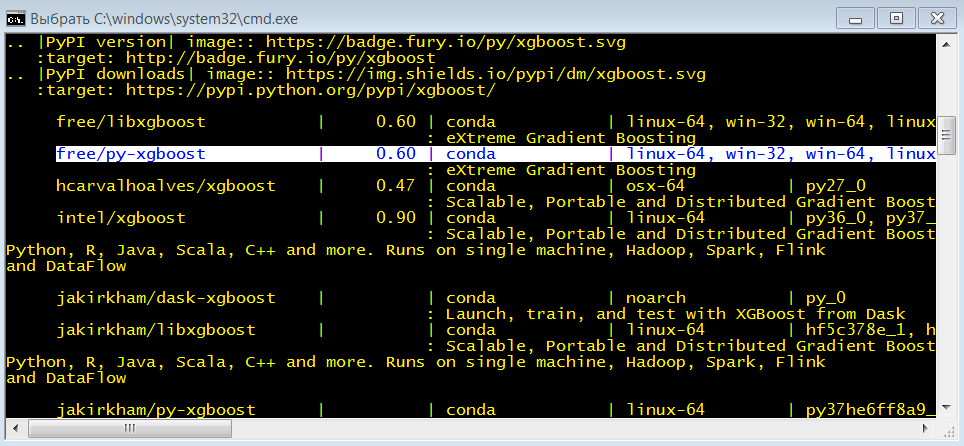
\includegraphics[scale=0.85]{figures/xgboost_conda_search.png}
	\caption{Окно командной оболочки \texttt{cmd.exe} со списком доступных каналов, по которым будет проводиться поиск пакета \texttt{xgboost} }\label{fig:xgboost_conda_search}
\end{figure}


После, выбрав канал, можно приступать к установке пакета

\begin{lstlisting}[
	numbers = none
	]
	conda install -c free py-xgboost
\end{lstlisting}

\subsubsection{Простой пример работы с \texttt{xgboost} и \texttt{shap}}

Решается задача бинарной классификации. Требуется построить модель, предсказывающую годовой доход заявителя по порогу \$50'000 (то есть больше или меньше \$50'000 зарабатывает заявитель в год). Используется набор данных  UCI Adult income

\begin{lstlisting}[
	style = ironpython,
	numbers = none
	]
	import xgboost
	import shap  # для оценки важности признаков вычисляются значения Шепли (Shapley value)
	import numpy as np
	import matplotlib.pyplot as plt
	from sklearn.model_selection import train_test_split
	
	shap.initjs()
	
	X, y = shap.datasets.adult()
	X_display, y_display = shap.datasets.adult(display=True)
	
	X_train, X_test, y_train, y_test = train_test_split(X, y, test_size=0.2, random_state=7)
	d_train = xgboost.DMatrix(X_train, label=y_train)
	d_test = xgboost.DMatrix(X_test, label=y_test)
	
	params = {
		'eta' : 0.01,
		'objective' : 'binary:logistic',
		'subsample' : 0.5,
		'base_score' : np.mean(y_train),
		'eval_metric' : 'logloss'        
	}
	model = xgboost.train(params, d_train,
	num_boost_round = 5000,  # число итераций бустинга
	evals = [(d_test, 'test')],
	verbose_eval=100,  # выводит результат на каждой 100-ой итерации бустинга
	early_stopping_rounds=20)
	
	xgboost.plot_importance(model)
\end{lstlisting}

На \pic{fig:xgboost_plot}, \pic{fig:xgboost_plot_cover} и \pic{fig:xgboost_plot_gain} изображены графики важности признаков.

\begin{figure}[h]
	\centering
	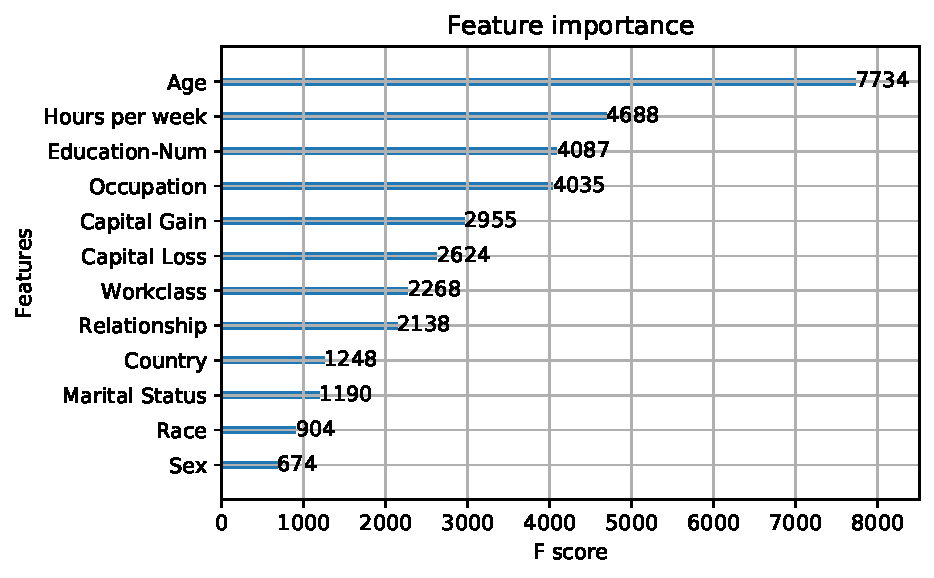
\includegraphics[scale=0.75]{figures/xgboost_plot.pdf}
	\caption{График важности признаков \lstinline{xgboost.plot_importance(model)},\\построенный с помощью пакета \texttt{xgboost} }\label{fig:xgboost_plot}
\end{figure}

\begin{figure}[h]
	\centering
	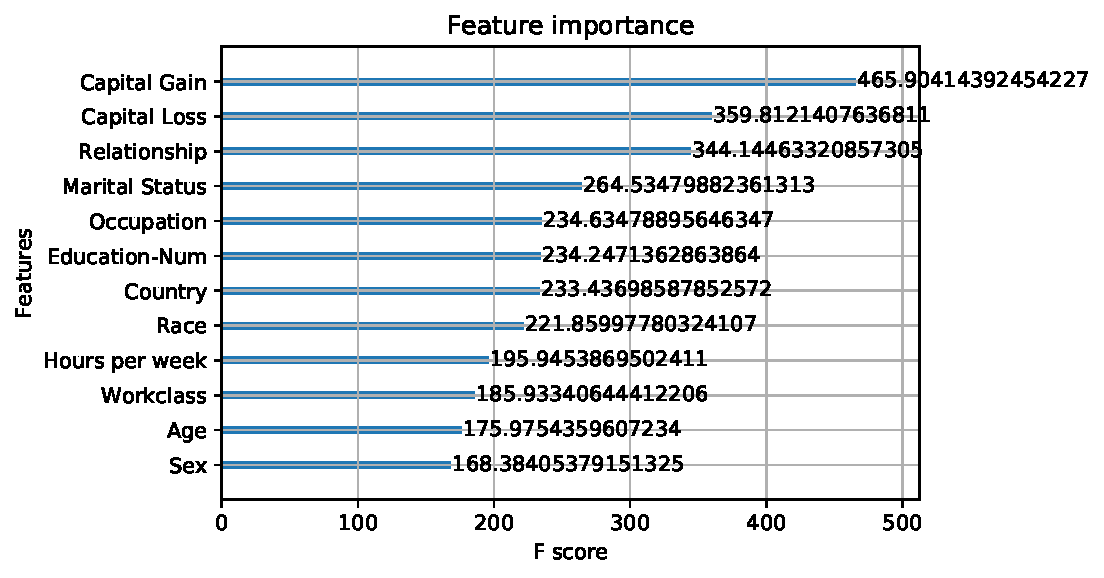
\includegraphics[scale=0.75]{figures/xgboost_plot_cover.pdf}
	\caption{График важности признаков \lstinline{xgboost.plot_importance(model, importance_type='cover')},\\построенный с помощью пакета \texttt{xgboost} }\label{fig:xgboost_plot_cover}
\end{figure}

\begin{figure}[h]
	\centering
	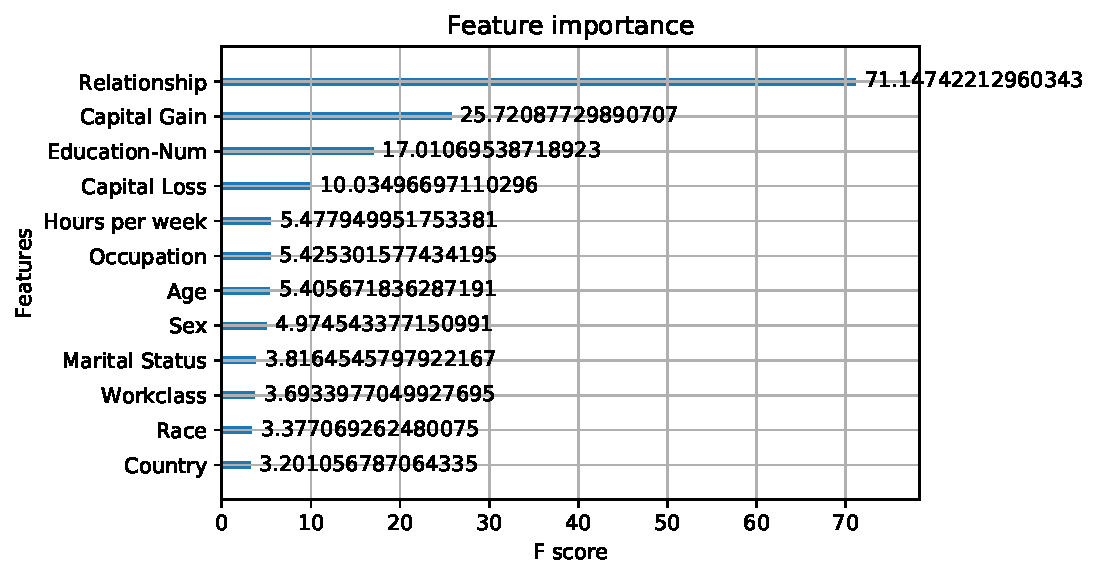
\includegraphics[scale=0.75]{figures/xgboost_plot_gain.pdf}
	\caption{График важности признаков \lstinline{xgboost.plot_importance(model, importance_type='gain')},\\построенный с помощью пакета \texttt{xgboost} }\label{fig:xgboost_plot_gain}
\end{figure}

Следует иметь в виду, что в библиотеке \texttt{xgboost} поддерживается три варианта вычисления важности признаков (см.~\href{https://towardsdatascience.com/interpretable-machine-learning-with-xgboost-9ec80d148d27}{Interpretable Machine Learning with XGBoost}):

\begin{itemize}
	\item \texttt{weight}: общее число сценариев по всем деревьям, когда $i$-ый признак используется для расщепления обучающего набора данных,
	
	\item \texttt{cover}: общее число сценариев по всем деревьям, когда $i$-ый признак используется для расщепления набора данных, взвешенное по числу точек обучающего набора данных, которые проходят через эти расщепления,
	
	\item \texttt{gain}: среднее снижение потерь на обучающем наборе данных, полученное при использовании $i$-ого признака.
\end{itemize}

Еще один простой типовой пример использования библиотеки \texttt{xgboost}
\begin{lstlisting}[
	style = ironpython,
	numbers = none
	]
	import xgboost
	from sklearn.datasets import load_boston
	from sklearn.model_selection import train_test_split
	from sklearn.model_selection import cross_val_score, KFold
	from sklearn.metrics import mean_squared_error
	
	boston = load_boston()
	X, y = boston.data, boston.target
	X_train, X_test, y_train, y_test = train_test_split(X, y, test_size=0.15, random_state=42)
	
	xgbr = xgboost.XGBRegressor(verbosity=0)
	xgbr.fit(X_train, y_train)
	
	score = xgbr.score(X_train, y_train)
	scores = cross_val_score(xgbr, X_train, y_train, cv=5)
	kfold = KFold(n_splits10, shuffle=True)
	kf_cv_scores = cross_val_score(xgbr, X_train, y_train, cv=kfold)
	
	y_pred = xgbr.predict(X_test)
	mse = mean_squared_error(y_test, y_pred)
\end{lstlisting}

\subsection{Регрессия}

Для простоты рассмотрим признаковое описание объекта с одним признаком Drug Dosage и целевой переменной Drug Effectiveness (см. \pic{fig:xgboost_train_data}).

\begin{figure}[h]
	\centering
	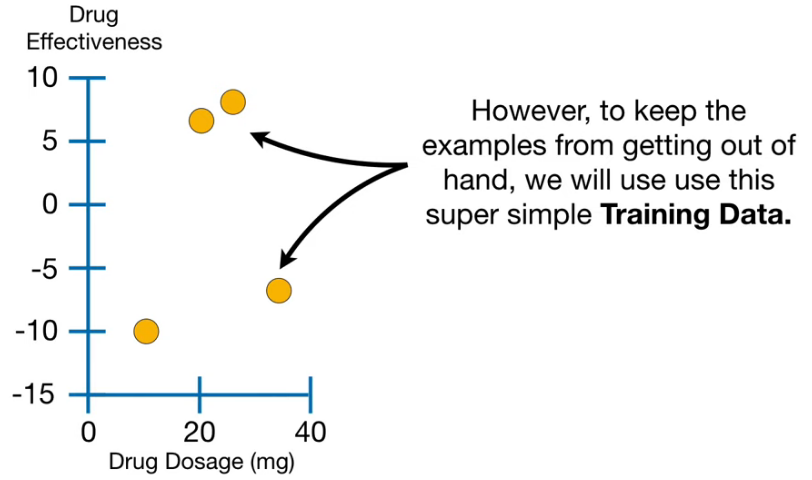
\includegraphics[scale=0.35]{figures/xgboost_train_data.png}
	\caption{ Простой набор данных }\label{fig:xgboost_train_data}
\end{figure}

На \pic{fig:xgboost_train_data} нижние две точки (большие отрицательные значения) отвечают низкой эффективности препарата, а верхние две точки, напротив, -- высокой эффективности.

На самом первом этапе построения дерева принятия решения в XGBoost задается \emph{базовое/начальное значение прогноза} (см. \pic{fig:xgboost_initial_pred}), которое по умолчанию принимается равным 0.5 независимо от того, для какой задачи используется XGBoost -- для регрессии или классификации.

\begin{figure}[h]
	\centering
	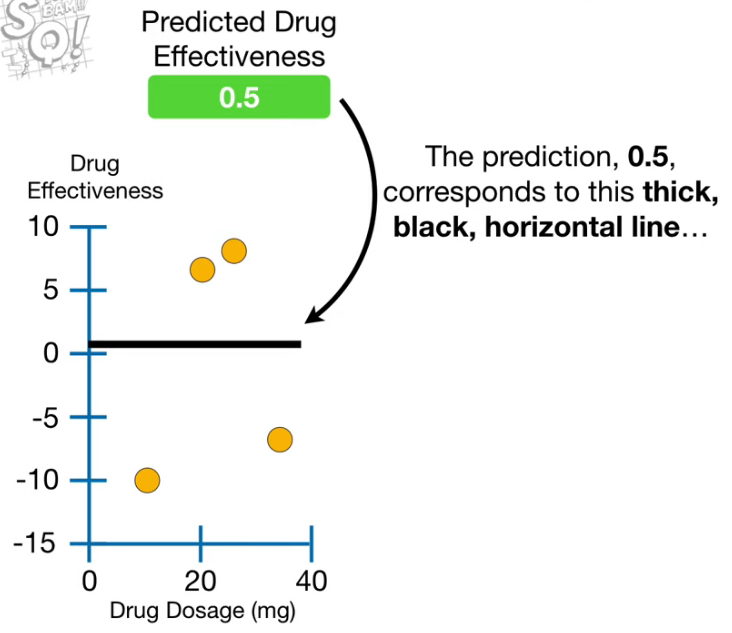
\includegraphics[scale=0.35]{figures/xgboost_initial_pred.png}
	\caption{ Базовое/начальное значение прогноза }\label{fig:xgboost_initial_pred}
\end{figure}

Далее вычисляются \emph{остатки} (residuals), которые представляют собой разность, составленную из наблюдаемых значений и значения прогноза (\pic{fig:xgboost_residuals})

\begin{figure}[h]
	\centering
	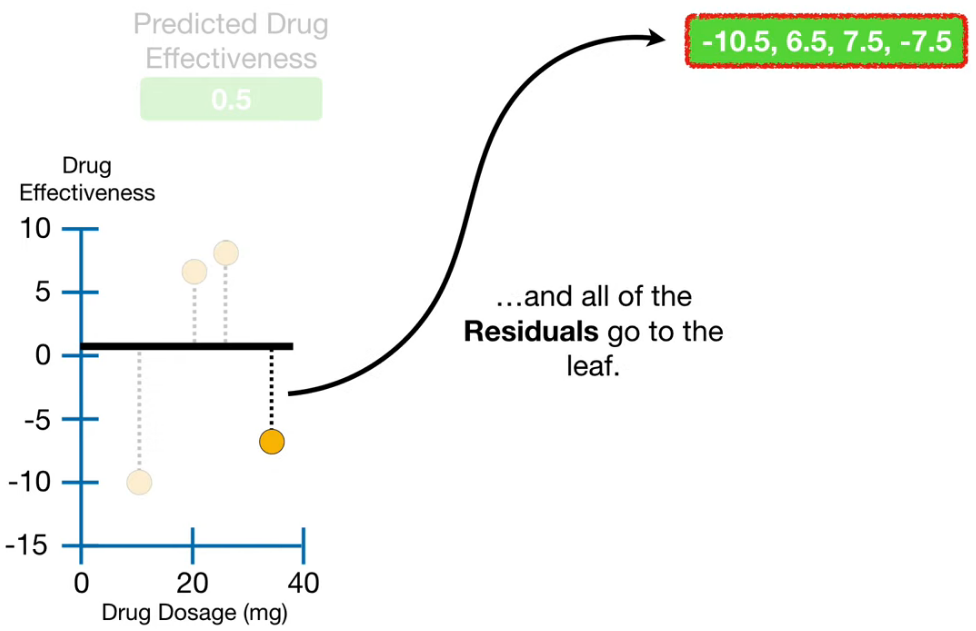
\includegraphics[scale=0.35]{figures/xgboost_residuals.png}
	\caption{ Остатки, как разность наблюдаемых значений и значения прогноза }\label{fig:xgboost_residuals}
\end{figure}

ВАЖНО: \emph{Экстремальный градиентный бустинг} как и \emph{классический градиентный бустинг} настраивается на \emph{\color{blue} остатки}, но в отличие от классического градиентного бустинга, который использует обычные деревья регрессии, экстремальный градиентный бустинг использует специальные XGBoost-деревья.

Существует множество способов построить XGBoost-дерево. Ниже приводится один из наиболее общих подходов к построению XGBoost-деревьев для задач регрессии.

Каждое дерево начинается с одиночного листа (узла), в которое попадают все остатки, т.е. разность между наблюдаемыми значениями и значением начального прогноза (\pic{fig:xgboost_residuals}).

Теперь можно вычислить \emph{сходство} (similarity score) на остатках по формуле (см. \pic{fig:xgboost_similarity})
\begin{align*}
	\text{similarity}_p = \dfrac{(\sum_{k}^{n} r_{k,p})^2}{n + \lambda},
\end{align*}
где $ r_{k,p} $ -- значения \emph{остатка}, по которому вычисляется сходство, в $ p $-ом родительском или дочернем узле бинарного дерева, $ n $ -- число точек, попавших в поднабор (например, если слева от порога оказалось 3 точки, то $ n = 3 $), $ \lambda $ -- параметр регуляризации (чем этот параметр больше, тем проще подрезать дерево, так как значения прироста получаются меньше).

\begin{figure}[h]
	\centering
	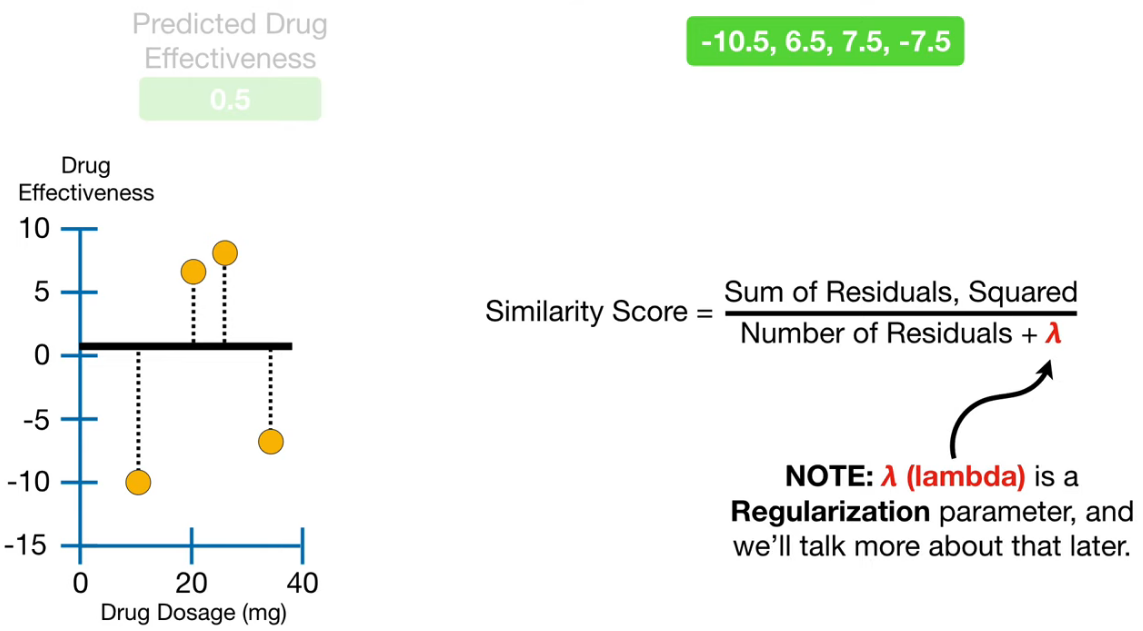
\includegraphics[scale=0.35]{figures/xgboost_similarity.png}
	\caption{ Вычисление сходства }\label{fig:xgboost_similarity}
\end{figure}

Например, сходство для родителького (в данном случае корневого) узла дерева при $ \lambda = 0 $ составит (\pic{fig:xgboost_similarity_4root})
\begin{align*}
	\text{similarity} = \dfrac{ (-10.5 + 6.5 + 7.5 + 7.5)^2 }{ 4 + 0} = 4.
\end{align*}

\begin{figure}[h]
	\centering
	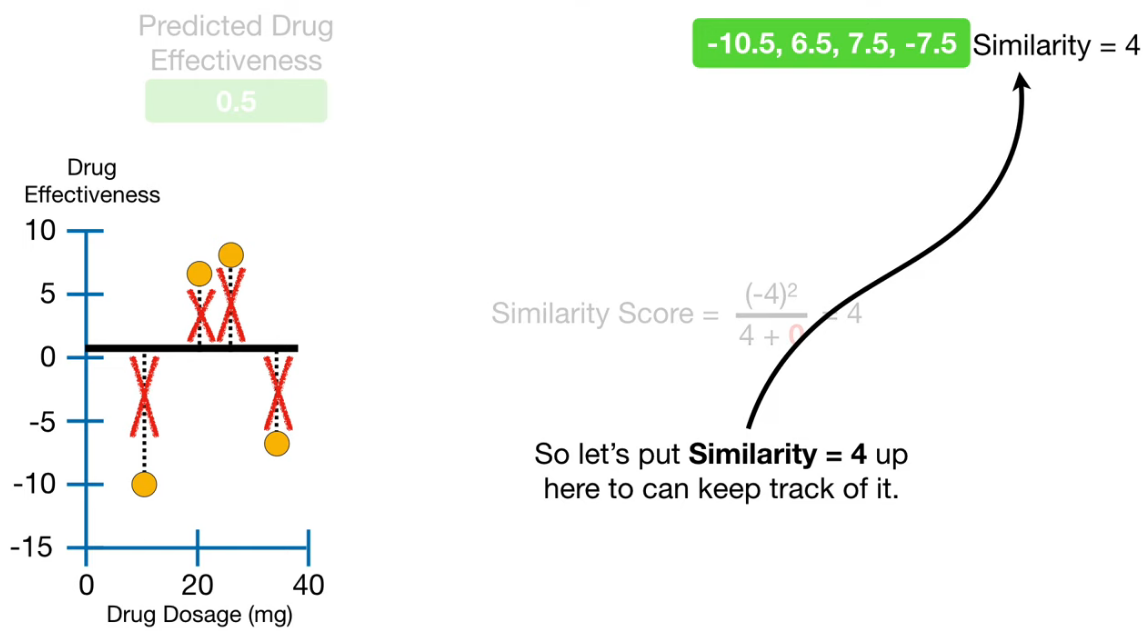
\includegraphics[scale=0.35]{figures/xgboost_similarity_4root.png}
	\caption{ Вычисление сходства для родительского узла дерева }\label{fig:xgboost_similarity_4root}
\end{figure}

Теперь надо ответить на вопрос о том сможем мы или нет повысить качество <<кластеризации>> таких остатков, если их разбить на две группы. Чтобы ответить на этот вопрос, начнем с самых нижних значений диапазона изменения признака Drug Dosage. Для первой пары значений признака Drug Dosage вычислим среднее -- $ \text{Drug Dosage} = 15 $ (\pic{fig:xgboost_dosage1}).

\begin{figure}[h]
	\centering
	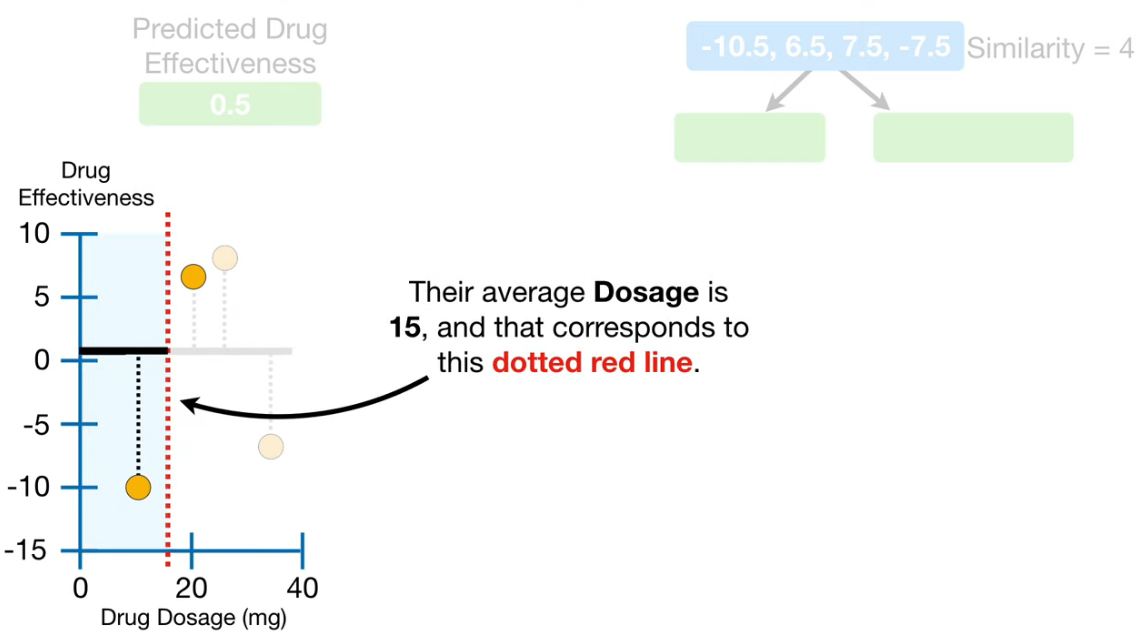
\includegraphics[scale=0.35]{figures/xgboost_dosage1.png}
	\caption{ Первый этап процедуры вычисления порога для признака Drug Dosage }\label{fig:xgboost_dosage1}
\end{figure}

Разобъем значения признака Drug Dosage по условию $ \text{Drug Dosage} < 15 $. В результате получится два листа -- в левый попадет только одно значение признака Drug Dosage, а в правый лист -- оставшиеся 3 (\pic{fig:xgboost_split1}). Можно вычислить сходство для дочерних узлов \pic{fig:xgboost_similarity_leaf1}.

\begin{figure}[h]
	\centering
	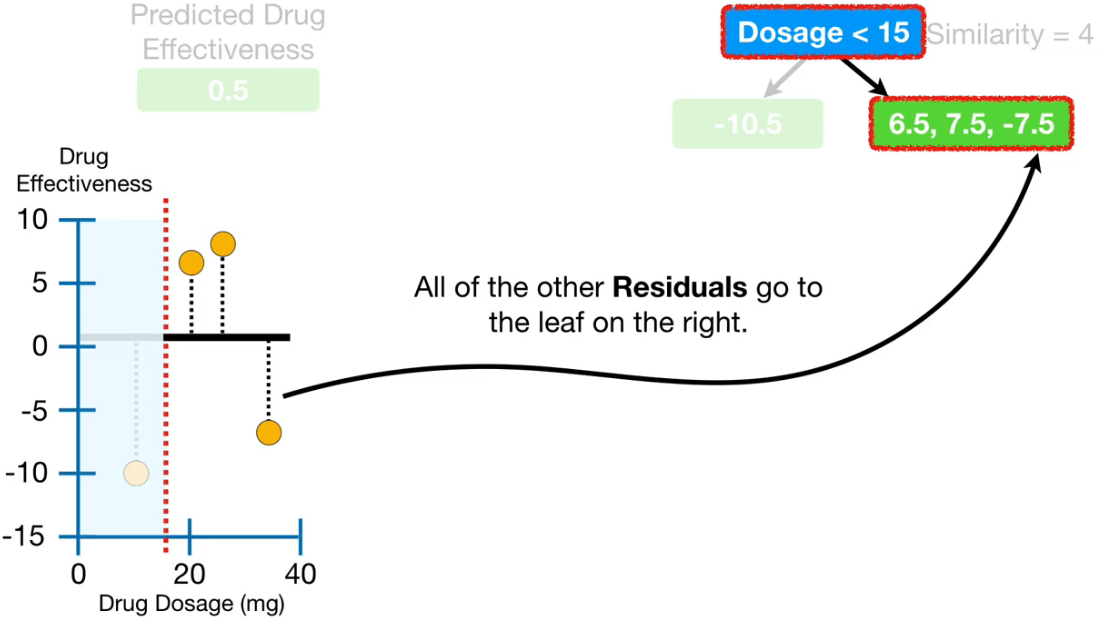
\includegraphics[scale=0.35]{figures/xgboost_split1.png}
	\caption{ Первое разбиение значений признака Drug Dosage }\label{fig:xgboost_split1}
\end{figure}

\begin{figure}[h]
	\centering
	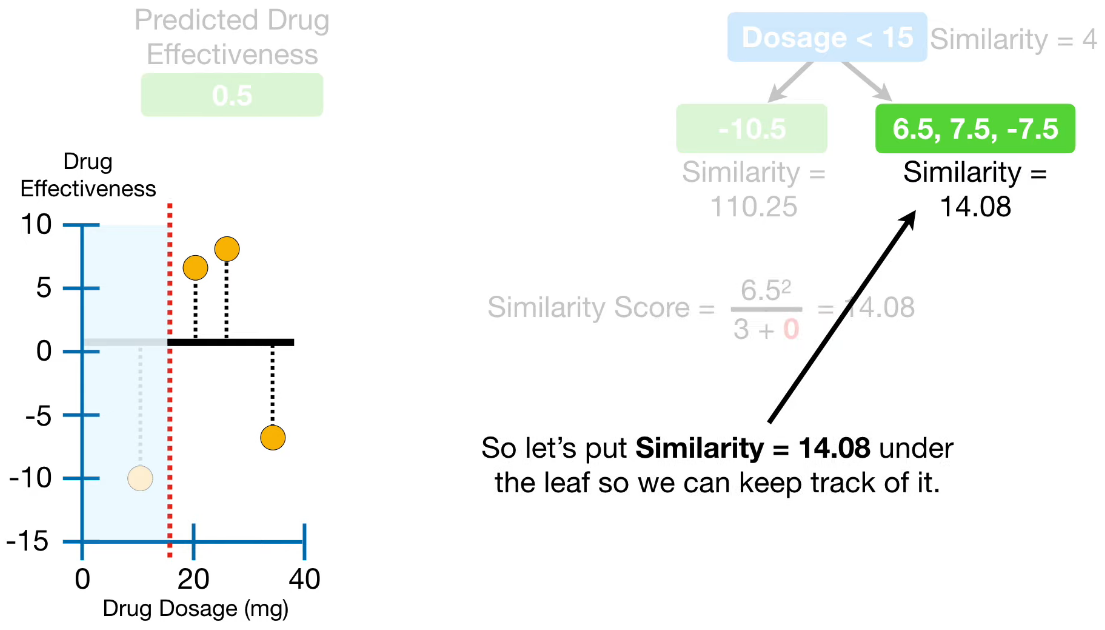
\includegraphics[scale=0.35]{figures/xgboost_similarity_leaf1.png}
	\caption{ Вычисление сходства для дочерних узлов }\label{fig:xgboost_similarity_leaf1}
\end{figure}

Когда узел состоит из сильно различающихся значений, то сходство для такого узла принимает небольшие значения, напротив, когда узел состоит из значений одного порядка (или только из одного значения), то сходство принимает большие значение.

ВАЖНО: мы ищем такое разбиение, при котором в дочерние узлы попадут экземпляры наиболее похожие друг на друга; например, в случае задачи регресии мы ищем такое разбиение, которое поместит экземпляры с остатками одного порядка в один и тот же дочерний узел

Теперь нужно количественно оценить насколько \emph{дочерние} узлы лучше \emph{группируют остатки}, чем родительский узел (\pic{fig:xgboost_gain1}).

\begin{figure}[h]
	\centering
	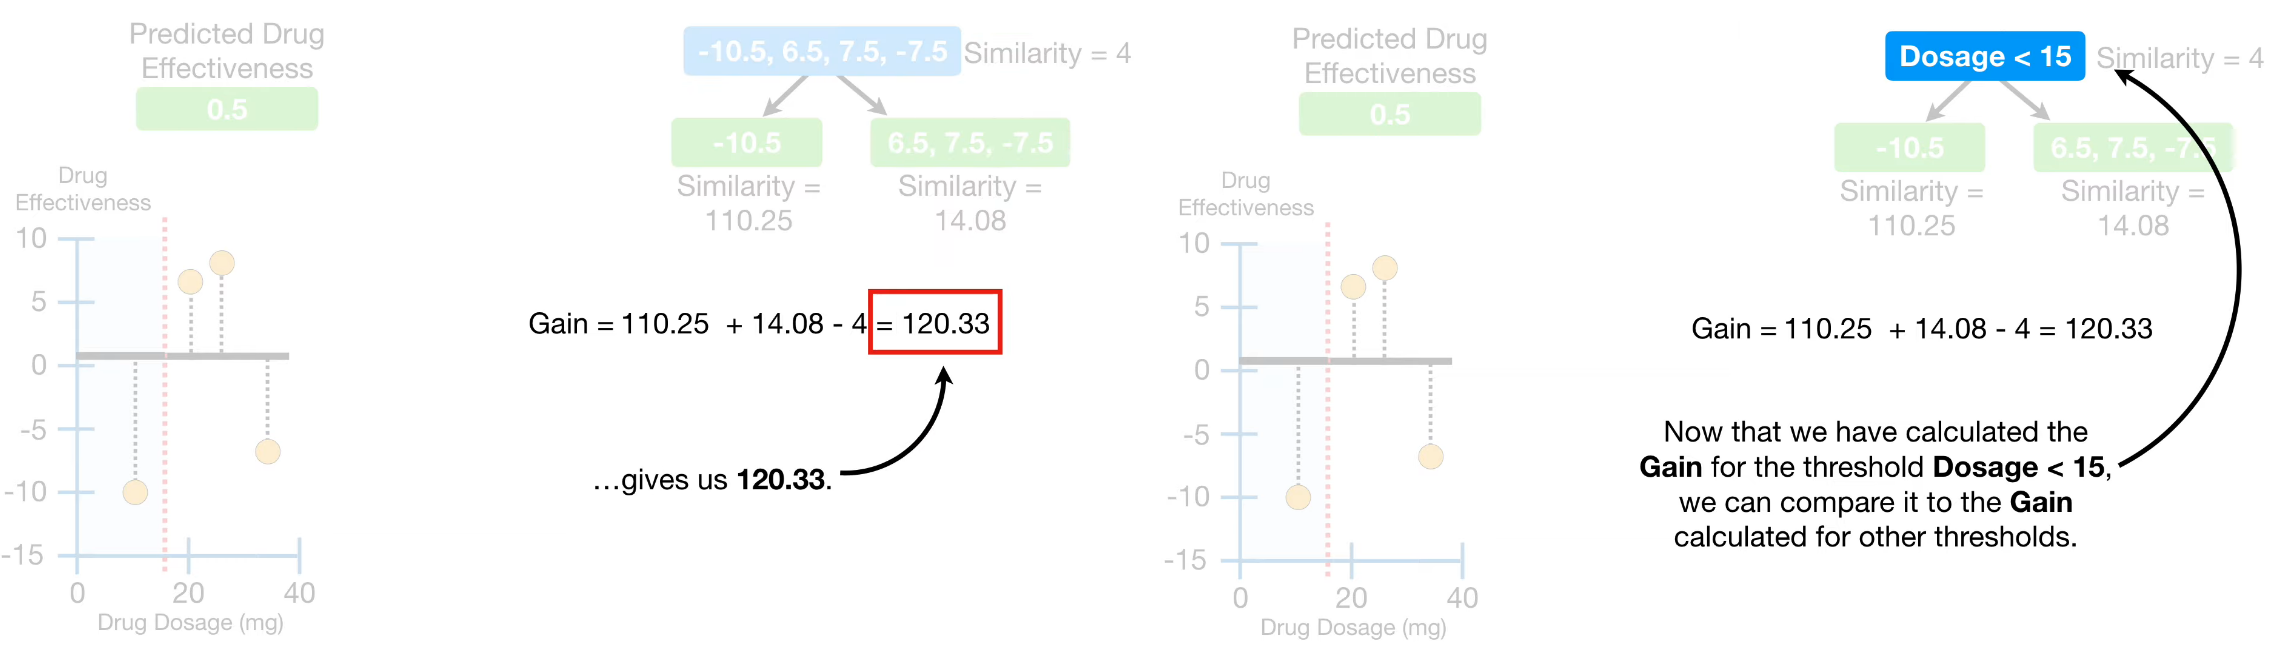
\includegraphics[scale=0.35]{figures/xgboost_gain1.png}
	\caption{ Вычисление прироста }\label{fig:xgboost_gain1}
\end{figure}

Сделать это можно, вычислив прирост (gain). Вообще для каждого \emph{условия расщепления} $ t $ в дереве принятия решения (в случае задачи регрессии) для оценки качества группировки остатков в дочерних узлах вычисляется \emph{прирост}
\begin{align*}
	\text{gain}_t = \text{similarity}_{left} + \text{similarity}_{right} - \text{similarity}_{root},
\end{align*}
где $ \text{similarity}_p $ -- сходство для родительского узла, левого или правого узлов.

Располагая значением прироста, мы можем сравнить различные стратегии разбиения (по сути мы сравниваем разбиения при различных значениях порога). Смещаем порог вправо, вычисляя среднее значение признака Drug Dosage для следующей пары точек (\pic{fig:xgboost_threshold2}).

\begin{figure}[h]
	\centering
	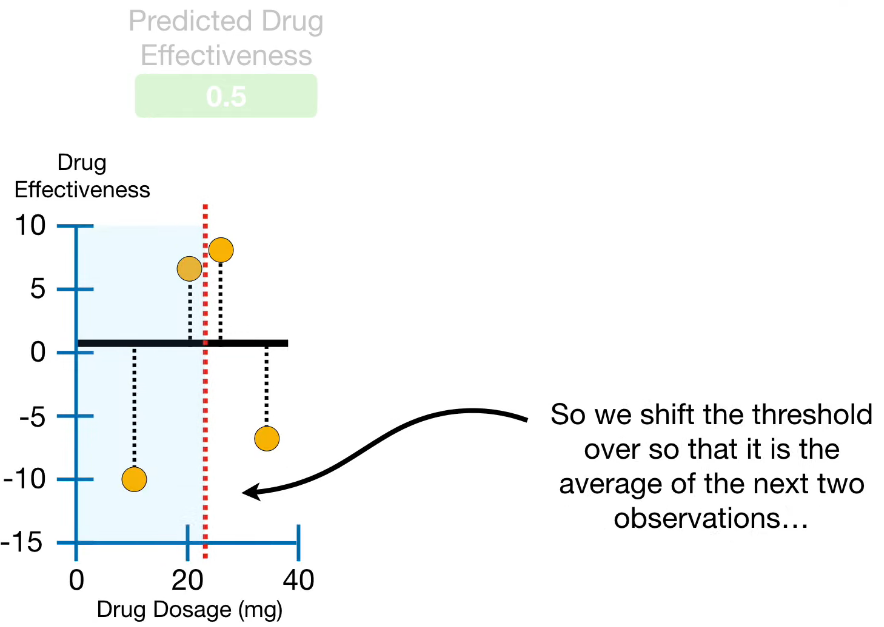
\includegraphics[scale=0.4]{figures/xgboost_threshold2.png}
	\caption{ Следующее разбиение признака Drug Dosage }\label{fig:xgboost_threshold2}
\end{figure}

Как в первый раз, строим дерево решения (\pic{fig:xgboost_split2}), но с новым значением порога ($ \text{Drug Dosage = 22.5} $).

\begin{figure}[h]
	\centering
	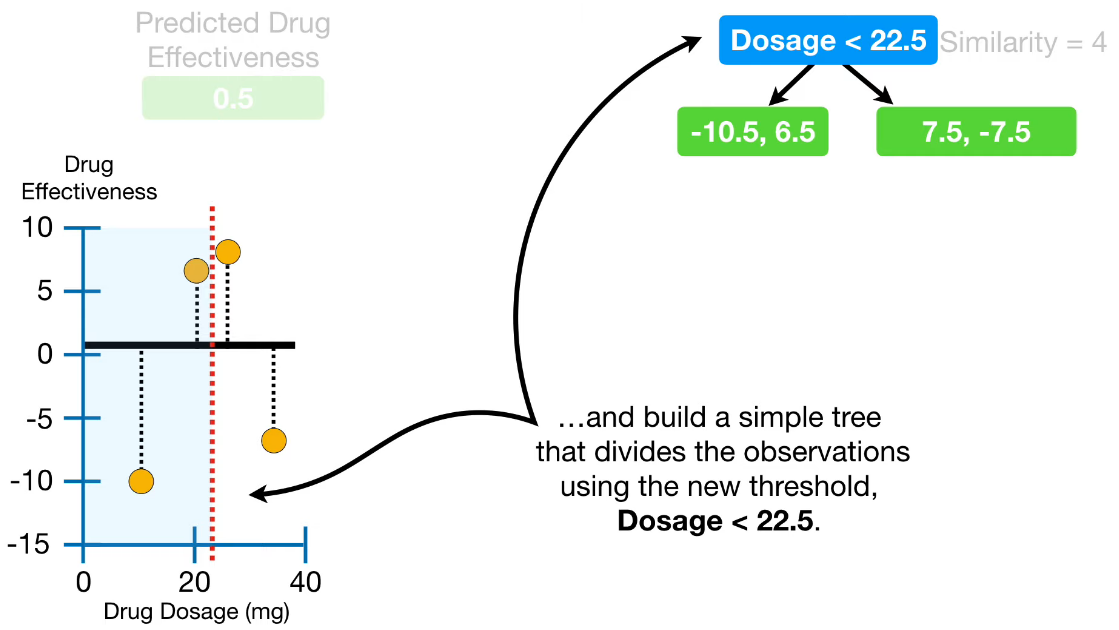
\includegraphics[scale=0.4]{figures/xgboost_split2.png}
	\caption{ Дерево решения для нового порога разбиения признака Drug Dosage }\label{fig:xgboost_split2}
\end{figure}

Снова вычисляем сходства для родительского и дочерних узлов, а затем прирост. Пусть на текущем этапе прирост составил 4, а не предыдущем шаге -- 120.3. Это означает, что разбиение по условию $ \text{Drug Dosage} < 15 $ ($ \text{gain} = 120.3 $) лучше кластеризует остатки, чем условие $ \text{Drug Dosage} < 22.5 $ ($ \text{gain} = 4 $).

Снова смещаем порог вправо, снова вычисляем сходства для родительского и дочерних узлов при разбиении по условию $ \text{Drug Dosage} < 30 $, снова находим прирост. Пусть в данном случае прирост составил 56.33. Значит, что как и раньше наилучшим разбиением является разбиение по условию $ \text{Drug Dosage} < 15 $ ($ \text{gain} = 120.3 $). 

Других пар точек у признака Drug Dosage нет, поэтому мы останавливаем процедуру выбора порога, а в качестве условия разбиения возьмем то, которому отвечает наибольшее значение \emph{прироста} (\pic{fig:xgboost_best_gain1}), т.е. $ \text{Drug Dosage} < 15 $ ($ \text{gain} = 120.3 $).

\begin{figure}[h]
	\centering
	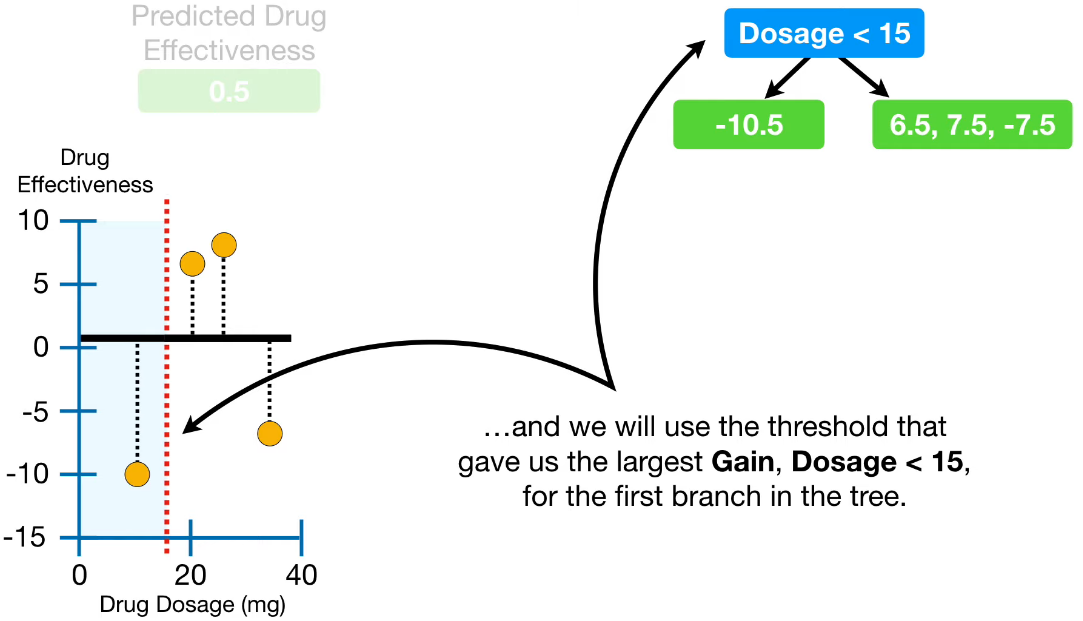
\includegraphics[scale=0.35]{figures/xgboost_best_gain1.png}
	\caption{ Наилучшее разбиение признака Drug Dosage по значению прироста }\label{fig:xgboost_best_gain1}
\end{figure}

В полученном разбиении в левом узле находится только один элемент и потому этот узел мы не можем разбивать дальше, но для правого узла можно поискать разбиение остатков (\pic{fig:xgboost_second_split}).

\begin{figure}[h]
	\centering
	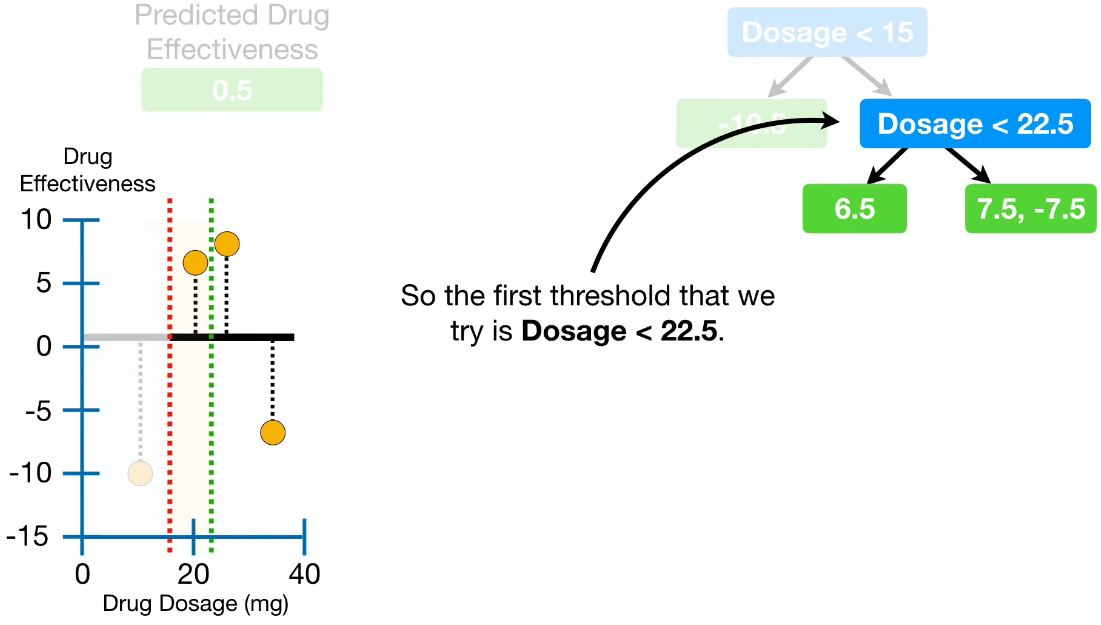
\includegraphics[scale=0.35]{figures/xgboost_second_split.png}
	\caption{ Начало процедуры поиска следующего лучшего разбиения для признака Drug Dosage }\label{fig:xgboost_second_split}
\end{figure}

Теперь, как раньше, вычисляем для разбиения по условию $ \text{Drug Dosage} < 22.5 $ сходство для дочерних узлов (сходство для родительского узла мы выясняли выше, когда вычисляли сходства для разбиения по условию $ \text{Drug Dosage} < 15 $ -- сходство составило 14.08). И вычисляем прирост. Он составил в данном случае 28.17 (\pic{fig:xgboost_gain2})

\begin{figure}[h]
	\centering
	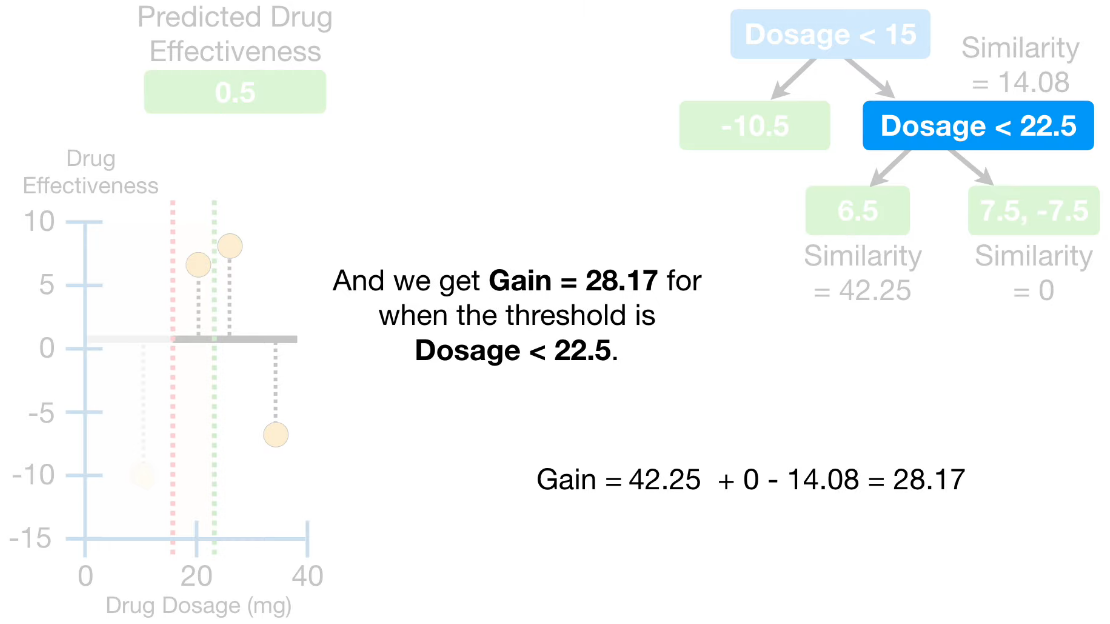
\includegraphics[scale=0.35]{figures/xgboost_gain2.png}
	\caption{ Вычисление прироста для второго разбиения признака Drug Dosage }\label{fig:xgboost_gain2}
\end{figure}

Смещаем порог вправо и повторяем процедуру с вычислением сходства и прироста. Пусть прирост для разбиения по условию $ \text{Drug Dosage} < 30 $ составил 140.17. Будем использовать разбиение $ \text{Drug Dosage} < 30 $ (\pic{fig:xgboost_best_split2}), как отвечающее наибольшему приросту ($ \text{gain} = 120.3 $).

\begin{figure}[h]
	\centering
	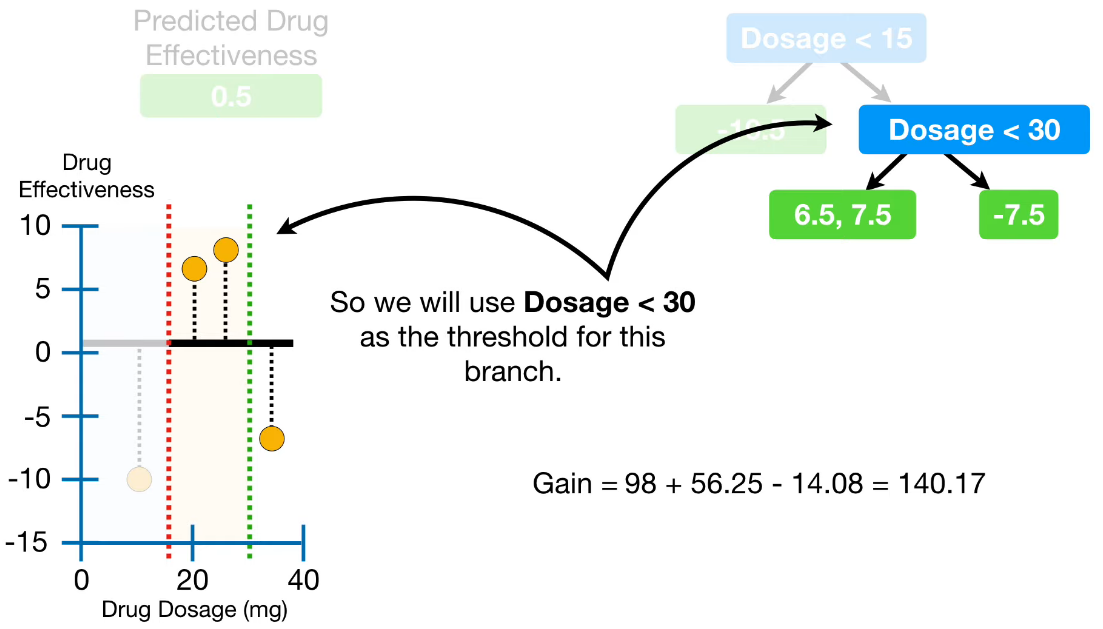
\includegraphics[scale=0.35]{figures/xgboost_best_split2.png}
	\caption{ Построение второго уровня дерева решений. Для простоты ограничиваемся двумя уровнями и не будем строить разбиение для левого узла }\label{fig:xgboost_best_split2}
\end{figure}

Для простоты ограничимся двумя уровнями дерева (по умолчанию дерево строится с 6 уровнями) и будем считать, что дерево решений построено.

Теперь стоит поговорить о \emph{подрезке} (prune). В XGBoost деревья подрезаются на основании значений прироста.


Для подрезания дерева принятия решения используется следующая стратегия. Задаются некоторым значением \emph{параметра сложности дерева} $ \gamma $ (например, $ \gamma = 130 $), а затем вычисляют $ \text{gain} - \gamma $, начиная с самой нижней ветки дерева. Если разность получается отрицательной, то ветку удаляют и поднимаются на следующий уровень, снова вычисляя $ \text{gain} - \gamma $ и т.д. Если разность положительная, то ветку не удаляют. Теоретически так можно дойти и до корня дерева. Если для корня дерева разность получается отрицательной, то корень удаляется и у нас остается только базовое прогнозное значение, которое мы задавали в самом начале процедуры построения дерева (0.5) и которое является довольно экстремальной подрезкой.

ВАЖНО: нулевое значение параметра $ \gamma $ не отменяет подрезки дерева! Положительные значения $ \lambda $ снижают эффект переобучения, так как параметр $ \lambda $ -- параметр регуляризации, а регуляризация нужно для упрощения модели.

\emph{Выходное значение} $ m $-ого \emph{листа} (output value) рассчитывается как
\begin{align*}
	\text{(output value)}_m = \dfrac{ \sum_{k}^{n} r_{k,m} }{n + \lambda}
\end{align*}

Очевидно, что при $ \lambda = 0 $ выходное значение (output value), представляет собой \emph{обычное среднее} по остаткам (\pic{fig:xgboost_output}).

\begin{figure}[h]
	\centering
	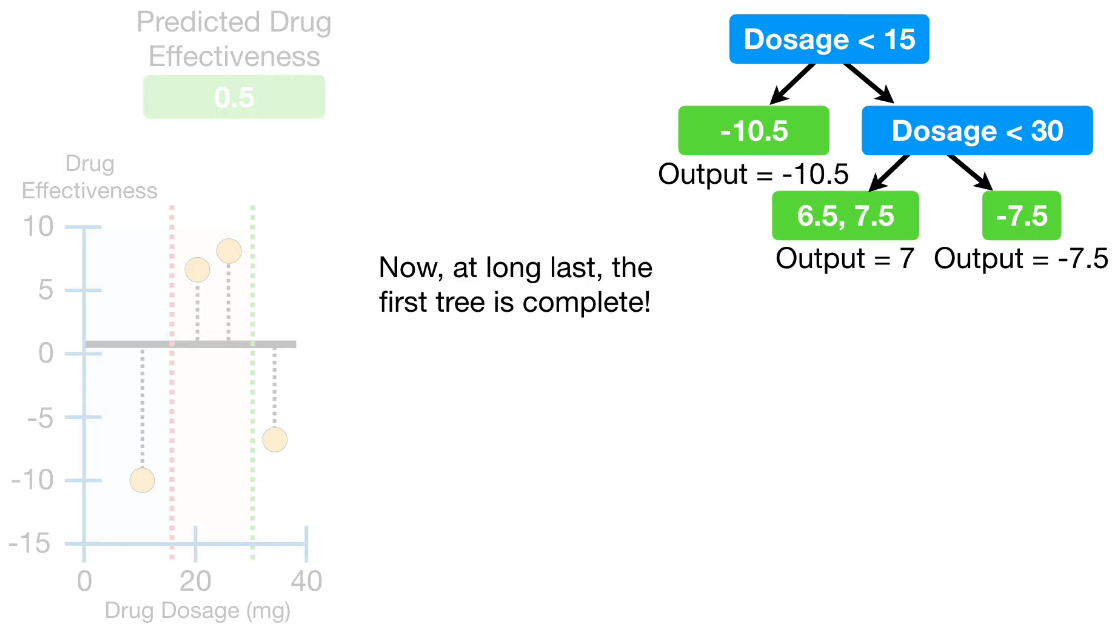
\includegraphics[scale=0.35]{figures/xgboost_output.png}
	\caption{ Выходы по листьям дерева }\label{fig:xgboost_output}
\end{figure}

Вычислить прогноз для конкретной точки на дереве экстремального градиентного бустинга (\pic{fig:xgboost_pred}), можно, как и в случае обычного градиентного бустинга, начав с базового прогноза (в данном случае 0.5) и добавив значение соответствующего листа (нужно пройти по всем условиям в дереве, используя указанные признаки и пороговые значения), умноженное на скорость обучения (learning rate)
\begin{lstlisting}[
style = bash,
numbers = none	
]
new_residual = 0.5 + learning_rate * output_value_from_leaf
\end{lstlisting}

Например, для листа с выходом -10.5 (значение признака Drug Dosage=10) прогноз будет $ 0.5 + 0.3 \cdot (-10.5) = -2.65 $. Тогда новое значение остатка на этой точке данных будет меньше чем раньше (\pic{fig:xgboost_pred2}). Аналогично можно вычислить прогноз (\pic{fig:xgboost_pred3}) для другого значения признака \texttt{Dosage} = 20: $ 0.5 + 0.3 \cdot 7 = 2.6 $ (было 6.5).

\begin{figure}[h]
	\centering
	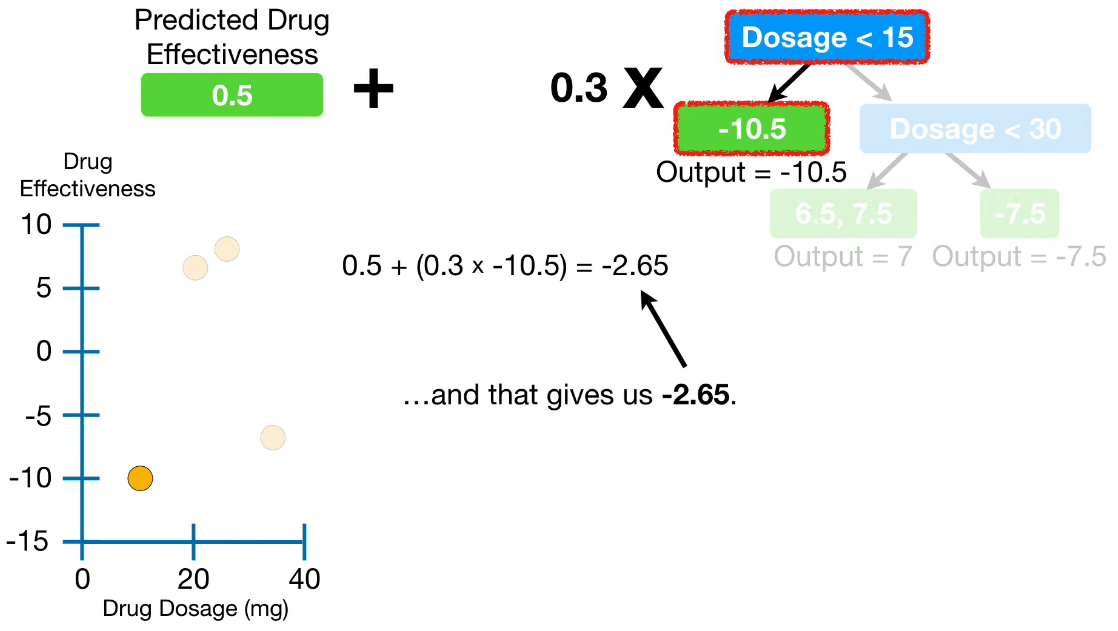
\includegraphics[scale=0.35]{figures/xgboost_pred.png}
	\caption{ Процедура построения прогноза в XGBoost для значения признака \texttt{Dosage=10} }\label{fig:xgboost_pred}
\end{figure}

\begin{figure}[h]
	\centering
	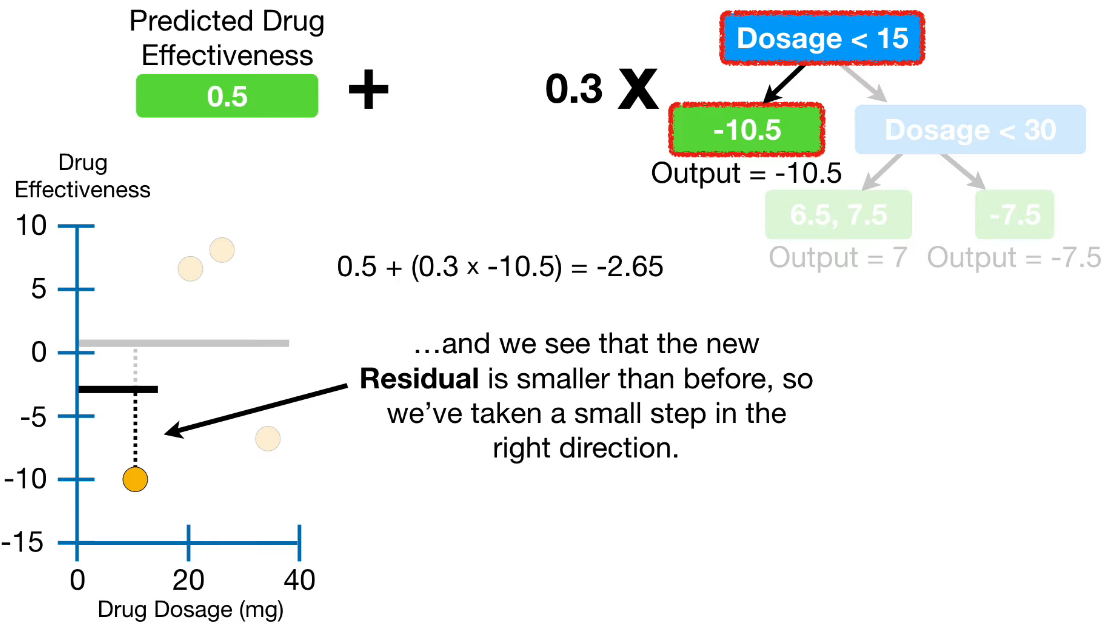
\includegraphics[scale=0.35]{figures/xgboost_pred2.png}
	\caption{ Остаток на точке \texttt{Dosage=10} стал меньше }\label{fig:xgboost_pred2}
\end{figure}

\begin{figure}[h]
	\centering
	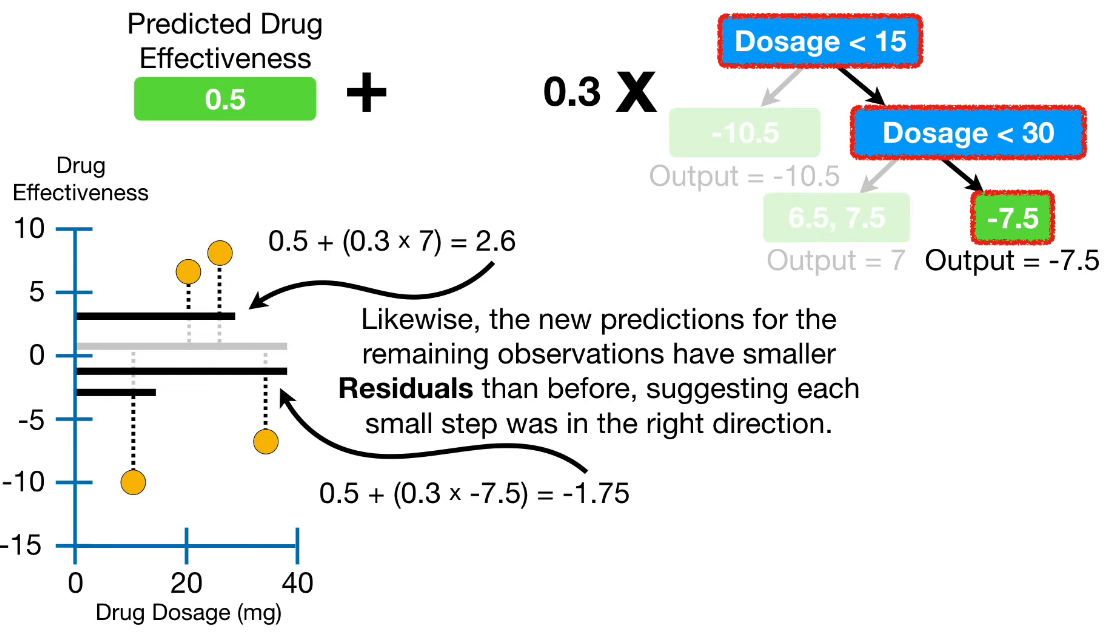
\includegraphics[scale=0.35]{figures/xgboost_pred3.png}
	\caption{ Остаток на точке \texttt{Dosage=20} стал меньше }\label{fig:xgboost_pred3}
\end{figure}

Теперь можно построить другое дерево на \emph{новых остатках} (residuals) и снова вычислить
\begin{lstlisting}[
style = bash,
numbers = none	
]
# предсказание -- это по сути новые остатки
prediction (new_residual) = 0.5 + learning_rate * output_value_from_leaf
\end{lstlisting}

Например, значения целевой переменной, отвечающей значению признака Dosage=10, с учетом новых значений остатков будет
$$
-2.65 + 0.3 \cdot (-10.5 + 2.65) = -5.005
$$

Мы продолжаем строить деревья до тех пор пока остатки не станут меньше заданного порога или пока мы не достигнем максимального числа итераций.

Порядок построения ансамбля деревьев экстремального градиентного бустинга для задач регрессии:
\begin{itemize}
	\item вычислить сходство (similarity score) для родительского, левого и правого узлов,
	
	\item вычислить прирост (gain) для соответствующего условия, ассоциированного с родительским узлом,
	
	\item вычислить разность между найденным значением прироста и заданным пользователем \emph{параметром сложности дерева} $ \text{gain} - \gamma $; если результат положительный, то подрезание (prune) дерева не выполняется, в противном случае выполняется,
	
	\item вычислить выходные значения листьев,
\end{itemize}

\subsection{Классификация}



\section{Потоки и процессы. Глобальная блокировка интерпретатора}

\emph{Процесс} -- просто программа в ходе ее выполнения. \emph{Потоки} подобны процессам, за исключением того, что все они выполняются в пределах одного и того же процесса, следовательно используют один и тот же контекст. 

Все потоки, организованные в одном процессе, используют общее пространство данных с основным процессом, поэтому могут обмениваться информацией или взаимодействовать друг с другом с меньшими сложностями по сравнению с отдельными процессами. Потоки, как правило, выполняются параллельно.

Если два или несколько потоков получают доступ к одному и тому же фрагменту данных, то в зависимости от того, в какой последовательности происходит доступ, могут возникать несогласованные результаты \cite[\strbook{184}]{chun:2015}.

Выполнением кода Python управляет виртуальная машина Python (называемая также \emph{главным циклом интерпретатора}). Язык Python разработан таким образом, чтобы в этом главном цикле мог выполняться \emph{только один поток управления}.

В интерпретаторе Python могут эксплуатироваться \emph{несколько потоков}, но в каждый отдельный момент времени интерпретатором выполняется \emph{строго один поток} \cite[\strbook{185}]{chun:2015}.

Для управления доступом к виртуальном машине Python применяется \emph{глобальная блокировка интерпретатора} (GIL). Именно эта блокировка обеспечивает то, что выполняется \emph{один и только один поток}.

Вообще говоря, применение нескольких потоков в программе может способствовать ее улучшению. Однако в интерпретаторе Python применяется глобальная блокировка, которая накладывает свои ограничения, поэтому \emph{многопоточная} организация является более подходящей для приложений, ограничиваемых пропускной способностью ввода-вывода\footnote{Так называемые IO-bound задачи} (при вводе-выводе происходит освобождение глобальной блокировки интерпретатора, что способствует повышению степени распараллеливания), а не приложений, ограничиваемых пропускной способностью процессора\footnote{CPU-bound задачи}. В последнем случае для достижения более высокой степени распараллеливания необходим иметь возможность \emph{параллельного выполнения процессов} несколькими ядрами или \emph{процессорами} \cite[\strbook{229}]{chun:2015}.

Глобальная блокировка GIL защищает состояние интерпретатора от вытесняющей (приоритетной многопоточности), когда один поток пытается взять на себя управление программой, прерывая другой поток. Если такое прерывание происходит в неподходящий момент времени, то это может разрушить состояние интерпретатора.

\textbf{Выводы}:
\begin{itemize}
	\item для приложений, ограниченных пропускной способностью ввода-вывода следует использовать
	\begin{itemize}
		\item многопоточность,
		
		\item приемы асинхронного программирования,
	\end{itemize}

    \item для приложений, ограниченных пропускной способностью процессора следует иметь возможность выполнения процессов несколькими процессорами.
\end{itemize}


\section{Форматирование строк в языке \texttt{Python}}

Пример форматирования строк в \texttt{Python} 

\begin{lstlisting}[
style = ironpython,
numbers = none
]
'{:*>+12.3f}, {:#^+17.5G}, {!r}'.format(
                                     math.pi,
                                     -math.exp(1)*10**(+6),
                                     type(list)  # для этого объекта будет
                                                 # использована функция repr()
                                 )
# "******+3.142, ###-2.7183E+06###, <class 'type'>"
\end{lstlisting}

Часть, стоящая после двоеточия, называется \emph{спецификатором формата} \cite[\strbook{283}]{ramalho:python-2016}. Полезные приемы форматирования можно найти в \cite{prohorenok:python-2016}.

В \texttt{Python} f-строки поддерживают вложенные элементы \verb|{...}|. Например, выведем числа $ n_i $ в едином формате, вычисляемые по формуле
$$
    n_i = (-1)^{i} \, \pi^{(-1)^i\,B}, \quad i = (1, \dots, m).
$$
\begin{lstlisting}[
style = ironpython,
numbers = none
]
import math

B = 15
for i in range(1, 5+1):
    n = (-1)**i*math.pi**((-1)**i*B)
    print(f'This is pi with {i} decimal places: {n:#>+15.{i}e}.')
    # вложенный элемент {...} может находится только в части спецификатора формата, после ':'
# вывод
This is pi with 1 decimal places: #######-3.5e-08.
This is pi with 2 decimal places: ######+2.87e+07.
This is pi with 3 decimal places: #####-3.489e-08.
This is pi with 4 decimal places: ####+2.8658e+07.
This is pi with 5 decimal places: ###-3.48941e-08.
\end{lstlisting}

\section{SSH-клиент в браузере}

В работе клиенты используют протокол SSH (Secure Shell) -- сетевой протокол, позволяющий осуществлять удаленное управление различными операционными системами. Поддерживает туннелирование TCP-соединений для передачи файлов и различные алгоритмы шифрования, благодаря чему возможна безопасная передача других протоколов через SSH-туннели.

Приложение \href{https://chrome.google.com/webstore/detail/secure-shell-app/pnhechapfaindjhompbnflcldabbghjo?hl=ru}{\ttfamily Secure Shell App} представляет собой эмулятор терминала, совместимый с xterm и SSH-клиент для Chrome. Он работает путем соединения SSH-команд, портированных в Google Native Client с эмулятором терминала hterm, что позволяет приложению предоставить клиенту Secure Shell прямо в браузере, не полагаясь на внешние прокси.

Установить SSH-клиент еще можно с помощью приложения \href{https://www.termius.com/}{Termius}. Поддреживает Windows, MacOS, Linux.


\section{Большие данные в Hadoop}

Hadoop это платформа для распределенного хранения и распределенной обработки больших данных.

\texttt{Hadoop} лучше всего подходит для:
\begin{itemize}
	\item Для хранения и обработки \emph{неструктурированных данных} объемом от \underline{1 терабайта} -- такие массивы сложно и дорого хранить в локальном хранилище,
	
	\item Для компонуемых вычислений -- когда нужно собрать множество схожих разрозненных данных в одно целое. Также подходит для выделения полезной информации из массива лишней информации,
	
	\item Для пакетной обработки, обогащения данных и ETL -- извлечения информации из внешних источников, ее переработки и очистки под потребности компании, последующей загрузки в базу данных.
\end{itemize}

\section{Теорема Байеса}

Пусть $ X $ -- случайная величина, ее возможное значение (или реализацию) будем обозначать через $ x $. Если $ \vec{X} = (X_1, \dots, X_n) $ -- случайный вектор, то его реализация -- $ \vec{x} = (x_1, \dots, x_n) $.

Для того чтобы охарактеризовать случайную величину, необходимо задать распределение вероятностей по ее возможным значениям. Для осуществления этого используется понятие \emph{функции распределения} вероятностей, которое является универсальным инструментом, пригодным для изучения любой случайной величины, одномерной или многомерной, и непрерывного, дискретного или смешанного типа.

Если $ X $ -- одномерная случайная величина непрерывного типа с бесконечным числом возможных значений на действительной оси $ \mathbb{R}^1 = \{x: -\infty < x < +\infty\} $, то она характеризуется функцией распределения вероятностей, которая определяется в виде
\begin{align*}
	F_X(x) = \mathbf{P}(X \leqslant x), \, x \in \mathbb{R}^1.
\end{align*}

Другими словами, функция распределения непрерывной случайной величины это вероятность события, состоящая в том, что случайная величина $ X $ примет значение меньшее или в частном случае равное некоторому значению $ x $, т.е. вероятность события, что случайная величина окажется левее.

Иногда удобнее описывать случайную величину $ X $ одномерной \emph{плотностью распределения вероятностей} $ f_X(x) = F_X^{'}(x), \, x \in \mathbb{R}^1 $ .

Для описания случайного вектора $ \vec{X} = (X_1, \dots, X_n) $ используют функцию $ n $ переменных, которая в точке $ (x_1, \dots, x_n) \in \mathbb{R}^n $, где $ \mathbb{R}^n $ обозначает $ n $-мерное евклидово пространство, определяется с помощью вероятности совместного осуществления событий в квадратных скобках, то есть функция распределения случайного вектора $ \vec{X} = (X_1, \dots, X_n) $ определяется в виде
\begin{align*}
	F_{X_1, \dots, X_n}(x_1, \dots, x_n) = F_{\vec{X}}(x_1, \dots, x_n) = \mathbf{P}[\,X_1 \leqslant x_1; X_n \leqslant x_n\,], \, (x_1, \dots, x_n) \in \mathbb{R}^n.
\end{align*}

Итак, для того чтобы охарактеризовать случайную величину $ X $, необходимо задать ее функцию распределения вероятностей.

Как известно, различают дискретные и непрерывные случайные величины. Две случайные величины называются \emph{независимыми}, если
\begin{align*}
	p(x,y) = p(x)p(y),
\end{align*}
где $ p(x) $ и $ p(y) $ -- плотности распределения непрерывных случайных величин.

Чтобы получить обратно из совместной вероятности вероятность того или иного исхода одной из случайных величин, нужно просуммировать по другой (этот процесс часто называют маргинализацией)
$$
p(x) = \sum_{y} p(x, y).
$$

В случае непрерывных случайных величин получается, что мы фактически проецируем двумерное распределение -- поверхность в трехмерном пространстве -- на одну из осей, получая функцию от одной переменной
$$
p(x) = \int_{Y} p(x, y)dy.
$$

\emph{Условная вероятность} $ p(x | y) $ -- вероятность наступления одного события, если известно, что произошло другое. Формально ее обычно определяют так
$$
p(x | y) = \dfrac{ p(x, y) }{p(y)}.
$$

Аналогично можно определить \emph{условную независимость}: $ x $ и $ y $ условно независимы при условии $ z $, если
\begin{align*}
	p(x, y | z) = p(x | z)p(y | z).
\end{align*}

\subsection{Регистрация пользовательских функций выхода из приложения}

Удобно использовать встроенный модуль \texttt{atexit} для регистрации пользовательских функций, которые вызываются при выходе из приложения. Например
\begin{lstlisting}[
style = ironpython,
numbers = none	
]
import atexit


def hello_fun():
    print('Hello message')

def exit_fun():
    print('New exit message')

atexit.register(exit_fun)
hello_fun()
\end{lstlisting}


\section{Глубокое обучение}

\subsection{Функции активации}

Без функции активации (например, такой как ReLU) полносвязный слой \texttt{keras.layers.Dense} сможет обучаться только на \emph{линейных} (аффинных) преобразованиях входнных данных: пространство гипотез было бы совокупностью всех возможных линейных преобразований входных данных.

Такое пространство гипотез слишком ограничено, и наложение нескольких слоев представлений друг на друга не приносило бы никакой выгоды, потому что \emph{глубокий стек линейных слоев} все равно реализует \emph{линейную операцию}: добавление новых слоев не расширяет пространство гипотез.

Чтобы получить доступ к более обширному пространству гипотез, дающему дополнительные выгоды от увеличения глубины представлений, необходимо применить \emph{нелинейную}, или функцию активации.

Наконец, нужно выбрать \emph{функцию потерь} и \emph{оптимизатор}. Пусть для определенности перед нами стоит задача бинарной классификации и результатом работы сети является вероятность (сеть заканчивается одномодульным слоем с сигмоидной функцией активации). В этом случае предпочтительнее использовать функцию потерь \texttt{binary\_crossentropy}. Перекрестная энтропия обычно дает более качественные результаты, когда результатами работы модели являются вероятности.

\emph{Перекрестная энтропия} -- мера расстояния между распределением вероятностей, или между фактическими данными и предсказаниями.

\begin{align*}
	H(p,q) \bydef H(p) + D_{KL}(p||q),
\end{align*}
где $ H(p) $ -- энтропия\footnote{Мера неопределенности некоторой системы} $ p $, $ D_{KL}(p||q) $ -- дивергенция Кульбака-Лейблера\footnote{Дивергенция Кульбака-Лейблера -- неотрицательнозначный фукнционал, являющийся несимметричной мерой удаленности друг от друга двух вероятностных распределений, определенных на общем пространстве элементарных событий} от $ p $ и $ q $ (она же относительная энтропия).

Для дискретных $ p $ и $ q $
\begin{align*}
	H(p,q) = - \sum_{x} p(x) \log q(x).
\end{align*}

Для непрерывного распределения
\begin{align*}
	H(p,q) = - \int_{X} p(x) \log q(x) dx.
\end{align*}

Нужно учесть, что, не смортя на формальную аналогию функционалов для непрерывного и дискретного случаев, они обладают разными свойствами и имеют разный смысл. Непрерывный случай имеет ту же специфику, что и понятие дифференциальной энтропии.

Настраиваем модель оптимизатором \texttt{rmsprop} и функцией потерь \texttt{binary\_crossentropy}
\begin{lstlisting}[
style = ironpython,
numbers = none
]
model.compile(optimizator='rmsprop',
              loss='binary_crossentropy',
              metrics=['accuracy'])
\end{lstlisting}

Или так, если нужно передать дополнительные параметры настройки
\begin{lstlisting}[
style = ironpython,
numbers = none
]
from keras import optimizers
from keras import metrics
from keras import losses
# настройка оптимизатора
model.compile(
    optimizer=optimizers.RMSprop(lr=0.001),
    loss='binary_crossentropy',
    metrics=['accuracy']
)

# использование нестандартных функций потерь и метрик
model.compile(
    optimizer=optimizers.RMSprop(lr=0.001),
    loss=losses.binary_crossentropy,
    metrics=[metrics.binary_crossentropy]
)
\end{lstlisting}

Чтобы проконтролировать точность модели во время обучения на данных, которые она прежде не видела, создадим проверочный набор данных, выбрав 10000 образцов из оригинального набора обучающих данных.
\begin{lstlisting}[
style = ironpython,
numbers = none
]
x_val = x_train[:10000]
partial_x_train = x_train[10000:]

y_val = y_train[:10000]
partial_y_train = y_train[10000:]
\end{lstlisting}

Теперь  проведем обучение модели в течение 20 эпох (выполнив 20 итераций по всем образцам в тензорах \texttt{x\_train}, \texttt{y\_train}) пакета по 512 образцов. В тоже время будем следить за потерями и точностью на 10000 отложенных образцах. Для этого достаточно передать проверочные данные в аргументе \texttt{validation\_data}
\begin{lstlisting}[
style = ironpython,
numbers = none
]
model.compile(
    optimizer='rmsprop',
    loss='binary_crossentropy',
    metrics=['acc']
)
history = model.fit(
    partial_x_train,
    partial_y_trian,
    epochs=20,  # 20 пробегов по обучающему набору данных
    batch_size=512,
    validation_data=(x_val, y_val) # вычисляем потерю и точность в конце каждой эпохи
)
\end{lstlisting}

\emph{В конце каждой эпохи} обучение приостанавливается, потому что модель вычисляет \emph{потерю} и \emph{точность} на 10000 образцах проверочных данных.

\subsection{Стохастический градиентный спуск}

Стохастический градиентный спуск это метод поиска \emph{локального} экстремума. Идея состоит в следующем:
\begin{itemize}
	\item Извлекается пакет обучающих экземпляров \texttt{x} и соответствующих целей \texttt{y},
	
	\item Сеть обрабатывает пакет \texttt{x} и получает пакет предсказаний \texttt{y\_pred},
	
	\item Вычисляются потери сети на пакете, дающие оценку несовпадания между \texttt{y\_pred} и \texttt{y},
	
	\item Вычисляется градиент потерь для параметров сети (обратных проход),
	
	\item Параметры корректируются на небольшую величину в направлении антиградиента, и тем самым снижают потери.
\end{itemize}

Сколько ни придумывай хитрых способов ускорить градиентный спуск, обойти небольшие локальные минимумы, выбраться из ущелий, мы все равно не сможем изменить тот факт, что градиентный спуск -- это метод местного значения, и ищет он только \emph{локальный} минимум/максимум.

Строго говоря, это реализация \emph{минипакетного стохастического градиентного спуска}. А истинный стохастический градиентный спуск на каждой итерации использует единственный образец и цель, а не весь пакет данных.

Здесь термин стохастический относится к тому, что \emph{каждый пакет} данных выбирается \emph{случайно}.

Обучим новую сеть с нуля 
\begin{lstlisting}[
style = ironpython,
numbers = none
]
model = models.Sequential()
model.add(layers.Dense(16, activation='relu', input_shape=(10000,)))
model.add(layers.Dense(16, activation='relu'))
model.add(layers.Dense(1, activation='sigmoid'))

model.compile(optimizer='rmsprop',
              loss='binary_crossentropy',
              metrics=['accuracy'])
              
model.fit(x_train, y_train, epochs=4, batch_size=512)
results = model.evaluate(x_test, y_test)

# сделать прогноз
model.predict(x_test)
\end{lstlisting}

В задачах бинарной классификации в конце нейросети должен находиться полносвязанный слой \texttt{Dense} с одним нейроном и функцией активации \texttt{sigmoid}: результатом работы сети должно быть скалярное значение в диапазоне между 0 и 1, представляющее собой вероятность.

С таким скалярным результатом, получаемым с помощью сигмоидной функции, в задачах бинарной классификации следует использовать функцию потерь \texttt{binary\_crossentropy}.

В общем случае оптимизатор \texttt{rmsprop} является наиболее подходящим выбором для любого типа задач.



\section{Хэшируемые пользовательские классы в языке \texttt{Python}}

Чтобы класс был хэшируемым\footnote{Обычно говорят, что объект называется хэшируемым если i) у него есть хэш-значение, которое не изменяется пока объект существует, и ii) объект поддерживает сравнение с другими объектами. Однако на мой взгляд лучше сказать, что объект является хэшируемым, если его структура не может изменяется и он поддерживает сравнение с другими объектами}, следует реализовать метод \texttt{\_\_hash\_\_}. Нужно также, чтобы векторы были \emph{неизменяемыми}. И этого можно добиться, сделав компоненты \texttt{x} и \texttt{y} свойствами, доступными только для чтения.

\begin{lstlisting}[
title = {\sffamily Пример неизменяемого, но нехэшируемого класса},
style = ironpython,
emph = {__init__, x, y, __iter__, __repr__, __str__, angle, __format__,
__bytes__, __eq__, __abs__, __bool__},
numbers = none
]
import array
import math

class Vector2d:
    '''
    Неизменяемый, но еще нехэшируемый класс
    '''
    typecode = 'd'

    def __init__(self, x, y):
        self.__x = x  # закрытый атрибут экземпляра класса
        self.__y = y  # закрытый атрибут экземпляра класса

    # открытое свойство; прочитать значение `x` можно, но нельзя передать новое значение
    @property  
    def x(self):
        return self.__x

    # открытое свойство; прочитать значение `y` можно, но нельзя передать новое значение
    @property  
    def y(self):
        return self.__y

    def __iter__(self):
        return (i for i in (self.x, self.y))

    def __repr__(self):
        class_name = type(self).__name__
        return '{}({!r}, {!r})'.format(class_name, *self)

    def __str__(self):
        return str(tuple(self))

    def angle(self):
        return math.atan2(self.y, self.x)

    def __format__(self, fmt_spec = ''):  # пользовательский формат
        if fmt_spec.endswith('p'):  # если спецификатор формата заканчивается на 'p',
                                    # то координаты выводятся в полярном формате
            fmt_spec = fmt_spec[:-1]
            coords = (abs(self), self.angle())
            outer_fmt = '<{}, {}>'
        else:
            coords = self
            outer_fmt = '({}, {})'
        components = (format(c, fmt_spec) for c in coords)
        return outer_fmt.format(*components)

    def __bytes__(self):
        return (bytes([ord(self.typecode)]) + bytes(array(self.typecode, self)))

    def __eq__(self, other):
        return tuple(self) == tuple(other)

    def __abs__(self):
        return math.hypot(self.x, self.y)

    def __bool__(self):
        return bool(abs(self))
\end{lstlisting}

То есть здесь декоратор \texttt{@property} помечает метод чтения свойств, который возвращает значение закрытого атрибута экземпляра класса \texttt{self.\_\_x} или \texttt{self.\_\_y}.

Так как в реализации класса есть метод \texttt{\_\_format\_\_}, можно печатать класс управляя форматом, например,

\begin{lstlisting}[
title = {\sffamily Пример использования класса с реализованным методом \texttt{\_\_format\_\_}},
style = ironpython,
numbers = none
]
>>> v1 = Vector2d(10, 5)
>>> '{:*^+12.3gp}'.format(v1)  # '<***+11.2****, ***+0.464***>'
>>> '{:.3f}'.format(v1)  # '(10.000, 5.000)'
\end{lstlisting}

Наконец, можно реализовать метод \texttt{\_\_hash\_\_}. Он должен возвращать \texttt{int} и в идеале учитывать хэши объектов-атрибутов, потому что у равных объектов хэши также должны быть одинаковыми.

В документации по специальному методу \texttt{\_\_hash\_\_} рекомендуется объединять хэши компонентов с помощью побитового оператора\footnote{Побитовые операторы рассматривают операнды как бинарные последовательности} \emph{исключающего ИЛИ} (\texttt{\^}) \cite[\strbook{287}]{ramalho:python-2016}

\begin{lstlisting}[
style = ironpython,
emph = {__hash__},
numbers = none
]
...
def __hash__(self):
    return hash(self.__x) ^ hash(self.__y)  # побитовое исключающее ИЛИ
\end{lstlisting}

Теперь класс \texttt{Vector2d} стал \emph{хэшируемым}.

\begin{lstlisting}[
style = ironpython,
numbers = none
]
>>> v1 = Vector2d(3, 4)
>>> v2 = Vector2d(3.1, 4.2)
>>> hash(v1), hash(v2)  # (7, 384307168202284039)
>>> set([v1, v2])  # {Vector2d(3, 4), Vector2d(3.1, 4.2)}
\end{lstlisting}

\remark{
Строго говоря, для создания хэшируемого типа необязательно вводить свойства или как-то иначе защищать атрибуты экземпляра класса от изменения. Требуется только корректно реализовать методы \texttt{\_\_hash\_\_} и \texttt{\_\_eq\_\_}. Но хэш-значения экземпляра никогда не должно изменяться \cite[\strbook{288}]{ramalho:python-2016}
}

\section{Как интерпретировать связь между именем функции и объектом функции в \texttt{Python}}

Рассмотрим класс, который печатает выводимые в терминал строки в обратном порядке

\begin{lstlisting}[
style = ironpython,
emph = {LookingGlass, __enter__, reverse_write, __exit__},
]
class LookingGlass:
    def __enter__(self):
        import sys
        # атрибут экземпляра класса self.original_write -> объект функции sys.stdout.write
        self.original_write = sys.stdout.write  
        # переменная sys.stdout.write -> объект функции self.reverse_write
        sys.stdout.write = self.reverse_write  
        return 'jabberwocky'.upper()
        
    def reverse_write(self, text):
        self.original_write(text[::-1])
        
        
    def __exit__(self, exc_type, exc_value, traceback):
        import sys
        # переменная sys.stdout.write "через" атрибут экземпляра self.original_write 
        # ссылается на объект функции sys.stdout.write
        sys.stdout.write = self.original_write
\end{lstlisting}

В методе \texttt{\_\_enter\_\_} есть несколько неочевидных нюансов. В строке 4 атрибут экземпляра класса \texttt{self.original\_write} получает ссылку на метод \texttt{write} стандартного потока вывода, а в строке 5 <<как бы метод>> \texttt{sys.stdout.write} получает ссылку на метод экземпляра класса \texttt{self.reverse\_write} и кажется, что должен был бы образоваться рекурсивный вызов, но на самом деле это не так. Дело в том, что значение имеет с какой стороны от оператора \texttt{=} стоит имя функции: если слева, то это \emph{имя переменной}, а если справа, то это \emph{объект функции}.

Итак, по порядку: в строке 4 атрибут экземпляра класса \texttt{self.original\_write} получает ссылку на \emph{объект функции} \texttt{sys.stdout.write}, а в 5-ой строке \emph{переменная} \texttt{sys.stdout.write} получает ссылку на \emph{объект функции} (метод экземпляра класса) \texttt{self.reverse\_write}, который <<через>> атрибут экземпляра \texttt{self.original\_write} вызывает \emph{объект функции} \texttt{sys.stdout.write}.

А в строке 18, мы возвращаем все как было, т.е. \emph{переменная} \texttt{sys.stdout.write} получает ссылку на \emph{объект функции} \texttt{sys.stdout.write}.

Рассмотрим более простой пример (см. \pic{fig:variable_with_link_function})

\begin{lstlisting}[
style = ironpython,
numbers = none
]
>>> def f(): pass  # переменная f -> объект функции f()
>>> def g(): pass  # переменная g -> объект функции g()
# модель: переменная -> объект
>>> a = f  # переменная a -> объект функции f()
>>> f = g  # переменная f -> объект фукнции g()
# НИКАКОЙ ТРАНЗИТИВНОСТИ!
>>> a  # <function __main__.f()>
>>> f  # <function __main__.g()>
\end{lstlisting}

То есть, когда объявляется функция, например, \texttt{def f(): pass}, то создается \emph{переменная} \texttt{f}, которая получает ссылку на \emph{объект функции} \texttt{f()}.

\remark{
Даже если используется одно и тоже имя \texttt{f}: слева от оператора присваивания \texttt{f} -- это \emph{переменная}, а справа от оператора \texttt{f} -- это \emph{объект} (например, объект функции), так как в \texttt{Python} переменные ссылаются только на объекты!
}

\begin{figure}[h]
	\centering
	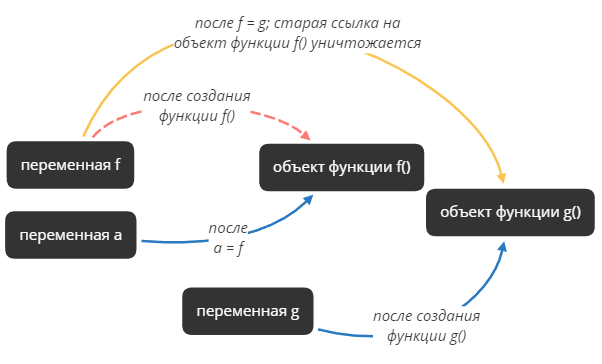
\includegraphics[scale=0.85]{figures/variable_with_link_function.png}
	\caption{ Схема, описывающая связи между именами функций и их объектами }\label{fig:variable_with_link_function}
\end{figure}

\section{Использование \texttt{@contextmanager}}

Если \emph{генератор} снабжен декоратором \texttt{@contextmanager}, то \texttt{yield} разбивает тело функции на две части:

\begin{itemize}
	\item все, что находится до \texttt{yield}, исполняется в начале блока \texttt{with}, когда интерпретатор вызывает метод \texttt{\_\_enter\_\_} ,
	
	\item а все, что находится после \texttt{yield}, выполняется при вызове метода \texttt{\_\_exit\_\_} в конце блока.
\end{itemize}

Например,

\begin{lstlisting}[
style = ironpython,
title = {\sffamily неудачный пример},
emph = {looking_glass, reverse_write}
]
# mirror_gen.py
import contextlib

@contextlib.contextmanager  # декорируем генераторную функцию
def looking_glass():  # генераторная функция
    import sys
    original_write = sys.stdout.write  # (1)
    
    def reverse_write(text):  # замыкание
        original_write(text[::-1])  # здесь original_write -- свободная переменная
    
    sys.stdout.write = reverse_write  # (2)
    # все что выше `yield` выполняется в начале блока with
    yield 'jabberwocky'.upper()  # (3)
    # все что ниже `yield` выполняется в конце блока with
    sys.stdout.write = original_write  # (4)
\end{lstlisting}

Комментарии к коду:

\begin{itemize}
	\item (1) -- локальная \emph{переменная} \texttt{original\_write} получает ссылку на \emph{объект функции} (вернее на объект метода) стандартного потока вывода; теперь вызывая \texttt{original\_write} мы будет вызывать \texttt{sys.stdout.write},
	
	\item (2) -- переменная \texttt{write} из подмодуля \texttt{stdout} модуля \texttt{sys} получает ссылку на \emph{замыкание} \texttt{reverse\_write} (функцию с расширенной областью видимости, которая включает все неглобальные переменные); теперь, когда мы вызываем \texttt{sys.stdout.write} будет вызываться \\ \texttt{reverse\_write}, который в свою очередь будет вызывать \texttt{original\_write}, вызывающий метод \texttt{sys.stdout.write} и передавать ему обращенную строку,
	
	\item (3) -- здесь функция приостанавливается на время выполнения блока \texttt{with},
	
	\item (4) -- когда поток выполнения покидает блок \texttt{with} любым способом, выполнение функции возобновляется с места, следующего за \texttt{yield}; в данном случае восстанавливается исходный метод \texttt{sys.stdout.write}
\end{itemize}

Пример работы функции

\begin{lstlisting}[
style = ironpython,
numbers = none
]
>>> from mirror_gen import looking_glass

>>> with looking_glass() as what:
        print('Alice, Kitty and Snowdrop')  # pordwonS dna yttiK ,ecilA
        print(what)                         # YKCOWREBBAJ
\end{lstlisting}

По существу декоратор \texttt{@contextlib.contextmanager} обертывает функцию классом, который реализует методы \texttt{\_\_enter\_\_} и \texttt{\_\_exit\_\_}\footnote{Этот класс называется \texttt{\_GeneratorContextManager}}.

Метод \texttt{\_\_enter\_\_} этого класса выполняет следующие действия \cite[\strbook{488}]{ramalho:python-2016}:

\begin{enumerate}
	\item Вызывает \emph{генераторную функцию} \texttt{looking\_glass()}\footnote{При вызове генераторной функции возвращается объект-генератор} и запоминает объект-генератор (пусть называется \texttt{gen}),
	
	\item Вызывает \texttt{next(gen)}, чтобы заставить генератор выполнить код до предложения \texttt{yield},
	
	\item Возвращает значение, отданное \texttt{next(gen)}, чтобы его можно было связать с переменной в части \texttt{as} блока \texttt{with}, т.е. строка, отданная инструкцией \texttt{yield} связывается с переменной \texttt{what}.
\end{enumerate}

По завершении блока \texttt{with} метод \texttt{\_\_next\_\_} выполняет следующие действия:

\begin{enumerate}
	\item Смотрит, было ли передано исключение в параметре \texttt{exc\_type}; если да, вызывает \\ \texttt{gen.throw(exception)}, в результате чего строка в теле генераторной функции, содержащая \texttt{yield}, возбуждает исключение,
	
	\item В противном случае вызывает \texttt{next(gen)}, что приводит к выполнению части генераторной функции после \texttt{yield}.
\end{enumerate}

В рассмотренном примере есть очень серьезный дефект: если в теле блока \texttt{with} возникает исключение, то интерпретатор перехватывает его и повторно возбуждает в выражении \texttt{yield} внутри \texttt{looking\_glass}. Но здесь нет никакой обработки исключений, поэтому функция аварийно завершается, оставив систему в некорректном состоянии.

Более аккуратный вариант генераторной функции приведен ниже

\begin{lstlisting}[
title = {\sffamily Правильный вариант},
emph = {looking_glass, reverse_write},
style = ironpython,
numbers = none
]
# mirror_gen_exc.py
import contextlib

@contextlib.contextmanager
def looking_glass():  # здесь генераторная функция работает скорее как сопрограмма
    import sys
    original_write = sys.stdout.write  # переменная получает -> на объект функции write

    def reverse_write(text):  # замыкание
        original_write(text[::-1])

    sys.stdout.write = reverse_write  # переменная write получает -> на замыкание reverse_write
    msg = ''
    try:
        yield 'jabberwocky'.upper()  # отдает строку и переключается на блок with
    except ZeroDivisionError:
        msg = 'Пожалуйста не делите на ноль!'
    finally:  # выполняется в любом случае
        sys.stdout.write = original_write  # переменная write получает -> на объект функции write
        if msg:  # if msg != ''
            print(msg)
\end{lstlisting}

Пример выполнения

\begin{lstlisting}[
style = ironpython,
numbers = none
]
>>> from mirror_gen_exc import looking_glass
>>> with looking_glass() as what:
        print('aaaabb')  # bbaaaa
        print(5/0)       # Пожалуйста не делите на ноль!
\end{lstlisting}

\remark{
Отметим, что использование слова \texttt{yield} в генераторе, который используется совместно с декоратором \texttt{@contextmanager}, не имеет ничего общего с итерированием. В рассмотренных примерах генераторная функция работает скорее, как \emph{сопрограмма}: процедура, которая доходит до определенной точки, затем приостанавливается и дает возможность поработать клиентскому коду до тех пор, пока он не захочет возобновить выполнение процедуры с прерванного места
}

\section{Перегрузка операторов в языке \texttt{Python}}

Перегрузка операторов позволяет экземплярам классов участвовать в обычных операциях \cite{prohorenok:python-2016}.

Основы перегрузки операторов:

\begin{itemize}
	\item запрещается перегружать операторы для встроенных типов,
	
	\item запрещается создавать новые операторы, можно перегружать существующие,
	
	\item несколько операторов нельзя перегружать вовсе: \texttt{is}, \texttt{and}, \texttt{or}, \texttt{not} (на побитовые операторы это не распространяется)
\end{itemize}

Фундаментальное правило: инфиксный оператор всегда возвращает \emph{новый объект}, т.е. создает новый экземпляр (составные операторы изменяемых объектов возвращают \texttt{self}, т.е. изменяют левый операнд на месте).

Иначе говоря, в случае инфиксных операторов нельзя модифицировать \texttt{self}, а нужно создавать и возвращать новый экземпляр подходящего типа \cite[\strbook{405}]{ramalho:python-2016}.

\remark{
\emph{Инфиксные} операторы (\texttt{*}, \texttt{+} и т.д.) независимо от типа данных всегда возвращают \emph{новый объект}. \emph{Составные} операторы (\texttt{+=}, \texttt{*=} и пр.) для объектов \emph{неизменяемого} типа данных (кортежи, строки и пр.) возвращают новый объект, но в случае объектов \emph{изменяемого} типа данных (списки) -- изменяют объект на месте
}

\begin{lstlisting}[
style = ironpython,
title = {\sffamily Сравнение работы инфиксных и составных операторов},
numbers = none
]
# изменяемый объект
>>> lst = [100]  
>>> id(lst)  # 179426376
>>> lst = lst*2  # инфиксный оператор возвращает новый объект, поэтому id будет другим
>>> id(lst)  # 117159368 -- изменился
>>> lst  # [100, 100]
>>> lst *= 2  # но составной оператор для изменяемого объекта изменяет левый операнд на месте
>>> lst  # [100, 100, 100, 100]
>>> id(lst)  # 117159368 -- не изменился
# неизменяемый объект
>>> tpl = (100,)
>>> id(tpl)  # 114189896
>>> tpl = tpl*2  # инфиксный оператор вернет новый объект
>>> tpl  # (100, 100)
>>> id(tpl)  # 82350344 -- изменился
>>> tpl *= 2  # составной оператор создаст новый объект и перепривяжет его к tpl
>>> tpl # (100, 100, 100, 100)
>>> id(tpl)  # 93229768 -- изменился
\end{lstlisting}

При умножении \emph{последовательности} (списки, кортежи, строки) на \emph{целое число} создается копия последовательности заданное число раз, а затем копии склеиваются. 

Как читать выражения с математическими операторами:
\begin{itemize}
	\item Смотрим к какому классу относится оператор: \emph{инфиксному} или \emph{составному},
	
	\item Если оператор инфиксный, то независимо от того являются операнды изменяемыми или нет будет возвращен новый объект\footnote{При условии, что оператор в случае данных операндов имеет смысл},
	
	\item Если оператор составной, то нужно выяснить является левый операнд изменяемым или нет,
	\begin{itemize}
		\item левый операнд изменяемый: составной оператор изменит левый операнд на месте (идентификатор не изменится),
		
		\item левый операнд неизменяемый: составной оператор создаст новый объект и перепривяжет его к переменной (изменится идентификатор).
	\end{itemize}
\end{itemize}

\subsection{Перегрузка оператора сложения}

Для поддержки операций с объектами \emph{разных типов} в \texttt{Python} имеется особый механизм диспетчеризации для специальных методов, ассоциированных с инфиксными операторами.

Видя выражение \texttt{a + b}, интерпретатор выполняет следующие шаги:

\begin{itemize}
	\item Если у \texttt{a} есть метод \texttt{\_\_add\_\_}, вызвать \texttt{a.\_\_add\_\_(b)} и вернуть результат, если только он не равен \texttt{NotImplemented}\footnote{\texttt{NotImplemented} -- это значение-синглтон, которое должен возвращать специальный метод инфиксного оператора, чтобы сообщить интерпретатору, что не умеет обрабатывать данный операнд} (т.е. оператор не знает как обрабатывать данный операнд),
	
	\item Если у левого операнда \texttt{a} нет метода \texttt{\_\_add\_\_} или его вызов вернул \texttt{NotImplemented}, проверить, есть ли у правого операнда \texttt{b} <<правый>> метод \texttt{\_\_radd\_\_}\footnote{Иногда такие методы называют <<инверсными>> методами, но лучше их представлять как \emph{правые} методы, так как они вызываются от имени правого операнда}, и, если да, вызвать \texttt{b.\_\_radd\_\_(a)} и вернуть результат, если только он не равен \texttt{NotImplemented},
	
	\item Если у \texttt{b} нет метода \texttt{\_\_radd\_\_} или его вызов вернул \texttt{NotImplemented}, возбудить исключение \texttt{TypeError}.
\end{itemize}

Рассмотрим реализацию методов сложения для объектов

\begin{lstlisting}[
style = ironpython,
emph = {VectorUser, __add__, __radd__, __iter__, __init__, __repr__},
numbers = none
]
import itertools
import reprlib

class VectorUser:
    def __init__(self, seq):
        self._seq = array('d', seq)

    def __iter__(self):
        return iter(self._seq)

    def __repr__(self):
        components = reprlib.repr(self._seq)
        components = components[components.find('['):-1]
        return f'Vector({components})'

    def __add__(self, other):
        try:
            pairs = itertools.zip_longest(self, other, fillvalue=0.0)
            return VectorUser(a + b for a, b in pairs)  # возвращает новый экземпляр класса
        except TypeError:
            return NotImplemented

    def __radd__(self, other):
        return self + other
\end{lstlisting}

Как работает этот код. Рассмотрим случай, когда экземпляр класса \texttt{Vector} находится слева от оператора \texttt{+}

\begin{lstlisting}[
style = ironpython,
numbers = none
]
>>> v1 = VectorUser([3, 4, 5])
>>> v1 + (10, 20, 30)  # Vector([13.0, 24.0, 35.0])
# v1.__add__((10, 20, 30))
# удобно представлять VectorUser.__add__(v1, (10, 20, 30))
\end{lstlisting}

Первым делом интерпретатор пытается выяснить есть ли у левого операнда метод \texttt{\_\_add\_\_}. В данном случае у объекта \texttt{v1} есть такой метод, поэтому ничто не мешает вызвать его напрямую. Аргумент \texttt{self} метода \texttt{\_\_add\_\_} получает ссылку на \texttt{v1} (экземпляр класса \texttt{Vector}), а \texttt{other} -- ссылку на кортеж. Далее с помощью \texttt{zip\_longest} конструируется генератор кортежей, который в следующей строке используется в генераторном выражении при создании нового экземпляра класса \texttt{Vector} (оператор должен возвращать новый объект).

Теперь рассмотрим случай, когда экземпляр класса \texttt{VectorUser} находится справа от оператора \texttt{+}

\begin{lstlisting}[
style = ironpython,
numbers = none
]
>>> (10, 20, 30) + v1
\end{lstlisting}

И снова интерпретатор пытается выяснить есть ли у левого операнда метод \texttt{\_\_add\_\_}. У кортежа есть такой метод, но он не умеет работать с объектом \texttt{VectorUser} (возвращает \texttt{NotImplemented}).

Теперь интерпретатор проверяет есть ли у правого операнда <<правый>> метод \texttt{\_\_radd\_\_}. Правый операнд это экземпляр класса \texttt{VectorUser}, поэтому \texttt{v1.\_\_radd\_\_((10, 20, 30))} это то же самое что и \texttt{VectorUser.\_\_radd\_\_(v1, (10, 20, 30))}.

Другими словами, аргумент \texttt{self} метода \texttt{\_\_radd\_\_} получает ссылку на объект \texttt{v1}, а аргумент \texttt{other} -- ссылку на кортеж. И тогда в выражении \texttt{self + other}, которое возвращается методом \texttt{\_\_radd\_\_}, экземпляр класса \texttt{VectorUser} окажется слева от оператора \texttt{+}. Интерпретатор, встретив выражение \texttt{self + other}, начинает с поиска метода \texttt{\_\_add\_\_} у левого операнда и, найдя его, возвращает новый экземпляр класса \texttt{VectorUser(...)}.

\remark{
Еще раз: чтобы поддержать операции с \emph{разными типами}, мы возвращаем специальное значение \texttt{NotImplemented} -- не исключение, -- давая интерпретатору возможность попробовать еще раз: поменять операнды местами и вызывать специальный инверсный (правый) метод, соответствующий тому же оператору (например, \texttt{\_\_radd\_\_})
}

\subsection{Перегрузка оператора умножения на скаляр}

Рассмотрим в качестве примера умножение вектора \texttt{VectorUser} на скаляр

\begin{lstlisting}[
style = ironpython,
emph = {__mul__, __rmul__},
numbers = none
]
import numbers

# внутри класса VectorUser
def __mul__(self, scalar):
    if isinstance(scalar, numbers.Real):  # сравнение с абстрактным базовым классом
        return VectorUser(n*scalar for n in self)
    else:
        return NotImplemented

def __rmul__(self, scalar):
    return self*scalar
\end{lstlisting}

\begin{lstlisting}[
style = ironpython,
numbers = none
]
>>> v1 = VectorUser([3, 4, 5])
>>> v1*4  # Vector([12.0, 16.0, 20.0])
>>> 10*v1 # Vector([30.0, 40.0, 50.0])
\end{lstlisting}

В первом случае интерпретатор начинает с поиска метода \texttt{\_\_mul\_\_} у левого операнда. Метод найден, объект справа (число 4) действительно является экземпляром подкласса абстрактного базового класса \texttt{numbers.Real}. Значит теперь можно вернуть экземпляр \texttt{VectorUser}.

Во втором случае интерпретатор так же начинает с поиска метода \texttt{\_\_mul\_\_} у левого операнда и не находит его. Поэтому на следующем шаге ищется правый метод \texttt{\_\_rmul\_\_} у правого операнда. Теперь объект \texttt{v1} в выражении \texttt{self*scalar} стоит слева и потому в методе \texttt{\_\_rmul\_\_} аргумент \texttt{self} ссылается на \texttt{v1}, а \texttt{scalar} -- на \texttt{4}. Видя выражение \texttt{self*scalar} интерпретатор вызывает метод \texttt{\_\_mul\_\_}, который на этот раз выполняется без проблем.



\remark{
В общем случае, если прямой инфиксный метод (например, \texttt{\_\_mul\_\_}) предназначен для работы только с операндами того же типа, что и \texttt{self}, бесполезно реализовывать соответствующий инверсный метод (например, \texttt{\_\_rmul\_\_}), потому что он, по определению, вызывается, только когда второй операнд имеет другой тип \cite[\strbook{425}]{ramalho:python-2016}
}

\subsection{Операторы сравнения}

Обработка операторов сравнения (\texttt{==}, \texttt{!=}, \texttt{>}, \texttt{<=} и т.д.) интерпретатором \texttt{Python} похожа на обработку инфиксных операторов, но есть два важных отличия \cite[\strbook{417}]{ramalho:python-2016}:

\begin{itemize}
	\item для прямых и инверсных (правых) методов служит один и тот же набор методов; например, в случае оператора \texttt{==} как прямой, так и правый вызов обращаются к методу \texttt{\_\_eq\_\_}, но изменяется порядок аргументов.
	
	\item в случае \texttt{==} и \texttt{!=}, если инверсный (правый) вызов завершается ошибкой, то \texttt{Python} сравнивает идентификаторы объектов, а не возбуждает исключение (см.~\tblref{tab:operators_comp}).
\end{itemize}

\begin{table}[h]
	\centering
	\caption{\itshape Операторы сравнения. Инверсные (правые) методы вызываются, когда\\ прямой вызов вернул \texttt{NotImplemented}}\label{tab:operators_comp}
	%\renewcommand{\arraystretch}{1.05}
	\begin{tabular}{lllll}
		{Группа} & {Инфиксный} & Прямой вызов & Инверсный вызов & Запасной вариант \\
		{} & оператор & метода & метода & {} \\ \hline\hline
		Равенство & \texttt{a == b} & \texttt{a.\_\_eq\_\_(b)} & \texttt{b.\_\_eq\_\_(a)} & \texttt{return id(a) == id(b)} \\
		\rowcolor[gray]{0.96} {} & \texttt{a != b} & \texttt{a.\_\_ne\_\_(b)} & \texttt{b.\_\_ne\_\_(a)} & \texttt{return not (a == b)} \\
		\hline
		Порядок & \texttt{a > b} & \texttt{a.\_\_gt\_\_(b)} & \texttt{a.\_\_lt\_\_(b)} & \texttt{raise TypeError} \\
		\rowcolor[gray]{0.96} {} & \texttt{a < b} & \texttt{a.\_\_lt\_\_(b)} & \texttt{a.\_\_gt\_\_(b)} & \texttt{raise TypeError} \\
		{} & \texttt{a >= b} & \texttt{a.\_\_ge\_\_(b)} & \texttt{a.\_\_le\_\_(b)} & \texttt{raise TypeError} \\
		\rowcolor[gray]{0.96} {} & \texttt{a <= b} & \texttt{a.\_\_le\_\_(b)} & \texttt{a.\_\_ge\_\_(b)} & \texttt{raise TypeError}
	\end{tabular}
\end{table}

Однако поведение оператора \texttt{==} пользовательских классов зависит от реализации метода \texttt{\_\_eq\_\_}. Например, пусть есть класс \texttt{Vector}

\begin{lstlisting}[
style = ironpython,
emph = {__eq__},
numbers = none
]
# в классе Vector
def __eq__(self, other):
    if isinstance(other, Vector):
        return (len(self) == len(other) and all(a == b for a, b in zip(self, other)))
    else:
        return NotImpemented
\end{lstlisting}

и какой-то другой класс \texttt{Vector2d}

\begin{lstlisting}[
style = ironpython,
emph = {__eq__},
numbers = none
]
# в классе Vector2d
def __eq__(self, other):
    retrun tuple(self) == tuple(other)
\end{lstlisting}

Если теперь сравнить экземпляры этих классов

\begin{lstlisting}[
style = ironpython,
numbers = none
]
>>> v1 = Vector([1, 2])
>>> v2 = Vector2d(1, 2)
>>> v1 == v2  # True
\end{lstlisting}
то порядок действий будет следующим:

\begin{itemize}
	\item для вычисления \texttt{v1 == v2} интерпретатор вызовет \texttt{Vector.\_\_eq\_\_(v1, v2)},
	
	\item метод \texttt{Vector.\_\_eq\_\_(v1, v2)} видет, что \texttt{v2} не является экземпляром класса \texttt{Vector} и возвращает \texttt{NotImplemented},
	
	\item получив значение \texttt{NotImplemented}, интерпретатор вызывает метод \texttt{\_\_eq\_\_} правого операнда, т.е. \texttt{v2}: \texttt{Vector2d.\_\_eq\_\_(v2, v1)},
	
	\item \texttt{Vector2d.\_\_eq\_\_(v2, v1)} преобразует оба операнда в кортежи и сравнивает их, результат оказывается равен \texttt{True}.
\end{itemize}

Теперь рассмотрим сравнение с кортежем

\begin{lstlisting}[
style = ironpython,
numbers = none
]
>>> t = (1, 2)
>>> v1 == t  # False
\end{lstlisting}

В этом случае:

\begin{itemize}
	\item для вычисления \texttt{v1 == t} \texttt{Python} вызывает \texttt{Vector.\_\_eq\_\_(v1, t)},
	
	\item метод \texttt{Vector.\_\_eq\_\_(v1, t)} видит, что кортеж \texttt{t} не является экземпляром класса \texttt{Vector} и возвращает \texttt{NotImplemented},
	
	\item получив результат \texttt{NotImplemented}, интерпретатор вызывает метод \texttt{\_\_eq\_\_} правого объекта, т.е. \texttt{tuple.\_\_eq\_\_(t, v1)}
	
	\item но \texttt{tuple.\_\_eq\_\_(t, v1)} ничего не знает о классе \texttt{Vector}, и поэтому возвращает \texttt{NotImplemented},
	
	\item если правый вызов вернул \texttt{NotImplemented}, то \texttt{Python} в качестве последнего средства сравнивает идентификаторы объектов, что в данном случае возвращает \texttt{False}
\end{itemize}




 
\section{Области видимости в языке \texttt{Python}}

Когда мы говорим о поиске значения имени применительно к программному коду, под термином \emph{область видимости} подразумевается \emph{пространство имен} -- то есть место в программном коде, где имени было присвоено значение \cite{lutz:learningpython-2011}.

В любом случае область видимости переменной (где она может использоваться) всегда определяется местом, где ей было присвоено значение.

\remark{%
Термины <<\emph{область видимости}>> и <<\emph{пространство имен}>> можно использовать как синонимичные
}

При каждом вызове функции создается новое \emph{локальное пространство имен}. Это пространство имен представляет локальное окружение, содержащее имена параметров функции, а также имена переменных, которым были присвоены значения в теле функции.

По умолчанию операция присваивания создает локальные имена (это поведение можно изменить с помощью \texttt{global} или \texttt{local}).

Схема разрешения имен в языке \texttt{Python} иногда называется \emph{правилом LEGB}\footnote{Local, Enclosing, Global, Built-in} \cite[\strbook{477}]{lutz:learningpython-2011}:

\begin{itemize}
	\item Когда внутри функции выполняется обращение к неизвестному имени, интерпретатор пытается отыскать его в четырех областях видимости -- в \emph{локальной}, затем в \emph{локальной области любой объемлющей функции} или в выражении \texttt{lambda}, затем в \emph{глобальной} и, наконец, во \emph{встроенной}. Поиск завершается, как только будет найдено первое подходящее имя.
	
	\item Когда внутри функции выполняется операция присваивания \lstinline{a=10} (а не обращения к имени внутри выражения), интерпретатор всегда создает или изменяет имя в \emph{локальной области видимости}, если в этой функции оно не было объявлено глобальным или нелокальным.
\end{itemize}

Пример

\begin{lstlisting}[
style = ironpython,
numbers = none
]
# глобальная область видимости
X = 99  

def func(Y):  # Y и Z локальные переменные
    # локальная область видимости
    Z = X + Y # X - глобальная переменная
    return Z
    
func(1)  # Y = 1
\end{lstlisting}

Переменные \texttt{Y} и \texttt{Z} являются \emph{локальными} (и существуют только во время выполнения функции), потому что присваивание значений обоим именам осуществляется внутри определения функции: присваивание переменной \texttt{Z} производится с помощью инструкции \texttt{=}, а \texttt{Y} -- потому что аргументы всегда передаются через операцию присваивания.

Когда внутри функции выполняется операция присваивания значения переменной, она всегда выполняется в \emph{локальном пространстве имен функции}

\begin{lstlisting}[
style = ironpython,
emph = {f},
numbers = none
]
a = 10  # глобальная область видимости

def f():
    a = 100  # локальная область видимости
    return a
\end{lstlisting}

В результате переменная \texttt{a} в теле функции ссылается на совершенно другой объект, содержащий значение 100, а не тот, на который ссылается внешняя переменная.

Переменные во вложенных функциях привязаны к \emph{лексической области видимости}. То есть поиск имени переменной начинается в \emph{локальной области видимости} и затем последовательно продолжается во всех \emph{объемлющих областях видимости внешних функций}, в направлении от внутренних к внешним.

Если и в этих \emph{пространствах имен} искомое имя не будет найдено, поиск будет продолжен в \emph{глобальном пространстве имен}, а затем во \emph{встроенном пространстве имен}, как и прежде.

При обращении к локальной переменной до того, как ей будет присвоено значение, возбуждается исключение \texttt{UnboundLocalError}. Следующий пример демонстрирует один из возможных сценариев, когда такое исключение может возникнуть

\begin{lstlisting}[
style = ironpython,
emph = {foo},
numbers = none
]
i = 0
def foo():
    i = i + 1  # приведет к исключению UnboundLocalError
    print(i)
\end{lstlisting}

В этой функции переменная \texttt{i} определяется как \emph{локальная} (потому что внутри функции ей присваивается некоторое значение и отсутствует инструкция \texttt{global}).

При этом инструкция присваивания \lstinline{i = i + 1} пытается прочитать значение переменной \texttt{i} еще до того, как ей будет присвоено значение.

Хотя в этом примере существует глобальная переменная \texttt{i}, она не используется для получения значения. Переменные в функциях могут быть либо \emph{локальными}, либо \emph{глобальными} и не могут произвольно изменять \emph{область видимости} в середине функции.

\remark{
Оператор \texttt{global} делает локальную переменную в теле функции \emph{глобальной} и говорит интерпретатору чтобы тот не искал переменную в локальной области видимости текущей функции
}

Например, нельзя считать, что переменная \texttt{i} в выражении \lstinline{i + 1} в предыдущем фрагменте обращается к глобальной переменной \texttt{i}; при этом переменная \texttt{i} в вызове \texttt{print(i)} подразумевает локальную переменную \texttt{i}, созданную в предыдущей инструкции.

\quinta{%
	Когда интерпретатор, построчно сканируя тело функции \texttt{def}, натыкается на строку \texttt{i = i + 1}, он заключает что переменная \texttt{i} является \emph{локальной}, так как ей присваивается значение именно в теле функции. А когда функция вызывается на выполнение и интерпретатор снова доходит до строки \texttt{i = i + 1}, выясняется, что переменная \texttt{i}, стоящая в правой части, не имет ссылок на какой-либо объект и потому возникает ошибка \texttt{UnboundLocalError}
}

\section{Декораторы в \texttt{Python}}

\emph{Декораторы} выполняются \emph{сразу после} загрузки или импорта модуля, однако увидеть какие-либо изменения можно только в том случае, если декоратор явно взаимодействует с пользователем на <<верхнем уровне>>\footnote{Если декоратор простой одноуровневый, то под верхним уровнем понимается его локальная область видимости, а если декоратор содержит замыкание, то -- понимается область видимости объемлющей функции}, например, печатает строку в терминале.  \emph{Задекорированные} же { функции} выполняются строго в результате явного вызова \cite[\strbook{217}]{ramalho:python-2016}.

\subsection{Реализация простого декоратора}

Рассмотрим простой декоратор, который хронометритует каждый вызов задекорированной функции и печатает затраченное время

\begin{lstlisting}[
style = ironpython,
title = {\sffamily clockdeco.py, не очень удачный пример декоратора},
emph = {clock, clocked},
numbers = none
]
import time

def clock(func):
    print('test string from `clock`')  # <- строка будет выведена в терминал
                                       # сразу после загрузки модуля, который
                                       # импортирует данный декоратор
    def clocked(*args):  # замыкание
        t0 = time.perf_counter()  # запомнить начальный момент времени
        result = func(*args)  # вызвать функцию
        elapsed = time.perf_counter() - t0  # вычислить сколько прошло времени
        name = func.__name__
        arg_str = ', '.join(repr(arg) for arg in args)
        print(f'{elapsed}, {name}({arg_str}) -> {result}')
        return result  # вернуть результат
return clocked
\end{lstlisting}

Использование декоратора выглядит так

\begin{lstlisting}[
label = {lst:deco},
style = ironpython,
title = {\sffamily clockdeco\_demo.py},
emph = {simple_deco_1, simple_deco_2,
simple_func_1, simple_func_2, inner, snooze, factorial}
]
import time
from clockdeco import clock

def simple_deco_1(f): 
    '''
    Декоратор с замыканием
    '''
    def inner():
        print('test string from `simple_deco_1`')  # <- строка НЕ будет выведена
                                                   # после загрузке модуля
    return inner

def simple_deco_2(f):
    '''
    Простой одноуровневый декоратор
    '''
    print('test string from `simple_deco_2`')  # <- строка будет выведена в терминал
                                               # сразу после загрузки модуля
    return f

@simple_deco_1  # simple_func_1 = simple_deco_1(f=simple_func_1) -> inner
def simple_func_1():
    print('test string from `simple_func_1`')   

@simple_deco_2  # simple_func_2 = simple_deco_2(f=simple_func_2) -> simple_func_2
def simple_func_2():
    print('test string from `simple_func_2`')   

@clock  # snooze = clock(func=snooze) -> clocked
def snooze(seconds):
    time.sleep(seconds)

@clock
def factorial(n):
    return 1 if n < 2 else n*factorial(n-1)


if __name__ == '__main__':
    print('*'*10, 'Calling snooze(.123)')
    print('snooze_result = {}'.format(snooze(.123)))
    print('*'*10, 'Calling factorial(6)')
    print('6! = ', factorial(6))
    print(f'This is result from `simple_func_1`: {simple_func_1()}')
    print(f'This is result from `simple_func_2`: {simple_func_2()}')
\end{lstlisting}

\begin{lstlisting}[
title = {\sffamily Вывод clockdeco\_demo.py},
numbers = none
]
test string from `simple_deco_2`
test string from `clock`
test string from `clock`
********** Calling snooze(.123)
0.1261, snooze(0.123) -> None
snooze_result = None
********** Calling factorial(6)
1.866e-06, factorial(1) -> 1
7.589e-05, factorial(2) -> 2
0.0001266, factorial(3) -> 6
0.0001732, factorial(4) -> 24
0.0002224, factorial(5) -> 120
0.0002715, factorial(6) -> 720
6! =  720
test string from `simple_deco_1`
this is result from `simple_func_1`: None
test string from `simple_func_2`
this is result from `simple_func_2`: None
\end{lstlisting}

\remark{
Приведенный выше пример декоратора \texttt{clock} из модуля \texttt{clockdeco.py} не удачен в том смысле, что если нам, например, потребуется вывести значение атрибута \texttt{\_\_name\_\_} задекорированной функции \texttt{snooze}, т.е. \texttt{snooze.\_\_name\_\_}, то будет возвращена строка \texttt{'clocked'}, а не \texttt{'snooze'}.

Чтобы декоратор <<не портил>> значения атрибута \texttt{\_\_name\_\_}, следует задекорировать замыкание декоратора с помощью \texttt{@functools.wraps(func)}
}


При разгрузке модуля \texttt{clockdeco\_demo.py} будут выполнены все декораторы, но только декораторы \texttt{simple\_deco\_2} и \texttt{clock} выведут в терминал строки, потому как эти строки расположены на верхнем уровне декораторов (т.е. находятся не внутри вложенных функций). Декоратор \texttt{simple\_deco\_1} ничего не выводит, так как строка находится в области видимости вложенной функции.

Важно отметить следующее: после загрузки модуля, как уже говорилось выше, будут выведены в терминал строки, расположенные на верхнем уровне декораторов, но самое главное заключается в том, что после выполнения декоратора \texttt{clock} объект \texttt{snooze} уже будет ссылаться на внутреннюю функцию \texttt{clocked} декоратора \texttt{clock}, а после выполнения декоратора \texttt{simple\_deco\_1} объект \texttt{simple\_func\_1} будет ссылаться на внутреннюю функцию \texttt{inner}. Что же касается декоратора \texttt{simple\_deco\_2}, то объект \texttt{simple\_func\_2} будет ссылаться на \texttt{simple\_func\_2}.

По этой причине при вызове функции \texttt{simple\_func\_1()} печатается строка из внутренней функции \texttt{inner}, а при вызове функции \texttt{simple\_func\_2()} -- строка из этой же функции.

Еще один пример декоратора с замыканием

\begin{lstlisting}[
style = ironpython,
emph = {deco, inner, target},
numbers = none
]
def deco(f):
    def inner(*args, **kwargs):
        print(f'from `deco-inner`: args={args}, kwargs={kwargs}')
        return f  # f - свободная переменная
    return inner

@deco  # target = deco(f=target) -> inner :: target -> inner :: target=inner
def target(a, b=10):
    return (f'from `target`: a={a}, b={b}')

print(target(20, b=500)(250))  # сначала вызывается inner(20, b=500), а потом target(250)
\end{lstlisting}

Выведет

\begin{lstlisting}[
numbers = none
]
from `deco-inner`: args=(20,), kwargs={'b': 500}
from `target`: a=250, b=10
\end{lstlisting}

\subsection{Кэширование с помощью \texttt{functools.lru\_cache}}

Декоратор \texttt{functools.lru\_cache} очень полезен на практике. Он реализует запоминание: прием оптимизации, смысл которого заключается в сохранении результатов предыдущих дорогостоящих вызовов функции, что позволяет избежать повторного вычисления с теми же аргументами, что и раньше \cite[\strbook{230}]{ramalho:python-2016}.

Например

\begin{lstlisting}[
style = ironpython,
emph = {fibonacci},
numbers = none
]
import functools
from clockdeco import clock

@functools.lru_cache
@clock
def fibonacci(n):
    if n < 2:
        return n
    return fibonacci(n-2) + fibonacci(n-1)
    
if __name__ == '__main__':
    print(fibonacci(6))
\end{lstlisting}

\remark{
\texttt{lru\_cache} хранит результаты в словаре, ключи которого составлены из позиционных и именованных аргументов вызовов, а это значит, что все аргументы, принимаемые декорируемой функции должны быть \emph{хешируемыми}
}

\subsection{Одиночная диспетчеризация и обобщенные функции}

Декоратор \texttt{functools.singledispatch} позволяет каждому модулю вносить свой вклад в общее решение. Обычная функция, декорированная \texttt{@singledispatch} становится \emph{обобщенной функцией}: групповой функцией, выполняющей одну и ту же логическую операцию по-разному в зависимости от типа первого аргумента \cite[\strbook{234}]{ramalho:python-2016}. Именно это и называется \emph{одиночной диспетчеризацией}. Если бы для выбора конкретных функций использовалось больше аргументов, то мы имели бы дело с \emph{множественной диспетчеризацией}.

Например

\begin{lstlisting}[
style = ironpython,
emph = {htmlize},
numbers = none
]
from functools import singledispatch
from collections import abc
import numbers
import html

@singledispatch  # делает функцию обобщенной
def htmlize(obj):
    content = html.escape(repr(obj))
    return '<pre>{}</pre>'.format(content)
    
    
@htmlize.register(str)  # будет вызываться для объектов строкового типа данных
def _(text):
    content = html.escape(text).replace('\n', '<br>\n')
    return '<p>{}</p>'.format(content)
    
    
@htmlize.register(numbers.Integral)  # будет вызваться для объектов целочисленного типа данных
def _(n):
    return '<pre>{} (0x{:x})</pre>'.format(n)
    
    
@htmlize.register(tuple)
@htmlize.register(abc.MutableSequence)
def _(seq):
    inner = '</li>\n<li>'.join(htmlize(item) for item in seq)
    return '<ul>\n<li>' + inner + '</li>\n</ul>'
\end{lstlisting}

\remark{
По возможности следует стараться регистрировать специализированные функции для обработки абстрактных базовых классов, например, \texttt{numbers.Integral} или \texttt{abc.MutableSequence}, а не конкретные реализации типа \texttt{int} или \texttt{list}
}

Замечательное свойство механизма \texttt{singledispatch} состоит в том, что специализированные функции можно зарегистрировать в любом месте системы, в любом модуле \cite{ramalho:python-2016}.

\subsection{Композиции декораторов}

Когда два декоратора \texttt{@d1} и \texttt{@d2} применяются к одной и той же функции \texttt{f} в указанном порядке, получается то же самое, что в результате композиции \texttt{f = d1(d2(f))}.

Иными словами

\begin{lstlisting}[
style = ironpython,
emph = {f},
numbers = none
]
@d1
@d2
def f():
    print('f')
\end{lstlisting}
эквивалентен следующему
\begin{lstlisting}[
style = ironpython,
emph = {f},
numbers = none
]
def f():
    print('f')
    
f = d1(d2(f))
\end{lstlisting}

Рассмотрим еще один пример композиции декораторов

\begin{lstlisting}[
style = ironpython,
emph = {deco1, deco2, target, inner1, inner2},
numbers = none
]
def deco1(f):  # выполняется вторым
    print('deco-1')  # # будет выведена в терминал
    def inner1():
        print('string from `deco1-inner`')
    return inner1

def deco2(f):  # выполняется первым
    print('deco-2')  # будет выведена в терминал
    def inner2():
        print('string from `deco2-inner')
    return inner2

@deco1  # 2) inner2 = deco1(f=inner2) -> inner1 :: inner2 -> inner1 :: inner2 = inner1
@deco2  # 1) target = deco2(f=target) -> inner2 :: target -> inner2 :: target = inner2
def target():  # 3) target -> inner1
    print('string from `target`')


if __name__ == '__main__':
    target()  # выведет string from `deco1-inner`
\end{lstlisting}

Выведет

\begin{lstlisting}[
numbers = none
]
deco-2
deco-1
string from `deco1-inner`
\end{lstlisting}

\remark{
Первым выполняется тот декоратор, который ближе расположен к декорируемой функции
}


То есть при загрузке или импорте модуля будут выполнены декораторы \texttt{deco1} и \texttt{deco2}: сначала \texttt{deco2}, а затем \texttt{deco1}, потому как \texttt{deco2} ближе к декорируемой функции. Декоратор \texttt{deco1} применяется к той функции, которую возвращает \texttt{deco2}.

\subsection{Параметризованные декораторы}

Параметризованные декораторы часто называют \emph{фабриками декораторов}. Фабрики декораторов возвращают настоящие декораторы, которые применяются к декорируемой функции.

Пример

\begin{lstlisting}[
style = ironpython,
emph = {register, decorate, f1, f2, f3},
numbers = none
]
registry = set()

def register(activate=True):  # фабрика декораторов
    def decorate(func):  # декоратор
        print(f'running register(activate={activate})->decorate({func})')
        if activate:
            registry.add(func)
        else:
            registry.discard(func)
        return func
    return decorate

@register(activate=False)  # f1 = decorate(func=f1) -> f1 :: f1 -> f1
def f1():
    print('running f1()')

@register()  # f2 = decorate(func=f2) -> f2 :: f2 -> f2
def f2():
    print('running f2()')

def f3():
print('running f3()')
\end{lstlisting}

Идея в том, что функция \texttt{register()} возвращает декоратор \texttt{decorate}, который затем применяется к декорируемой функции \cite{ramalho:python-2016}. 

\remark{
\emph{Фабрика декораторов} возвращает \emph{декоратор}, который применяется к декорируемой функции
}

Чуть подробнее: сразу после загрузки или импорта модуля выполняется фабрика декораторов \texttt{register}, которая возвращает декоратор \texttt{decorate}, который и применяется к функциям. Можно представлять, что фабрика декораторов нужна только для того, чтобы собрать значения каких-то дополнительных переменных, которые потребуются позже. В данном примере можно представить, что строка \texttt{@register()} заменяется на строку \texttt{@decorate}. То есть декоратор применяется к функции, расположенной на следующей строке, и работает как обычно.

Как можно работать с этой фабрикой декораторов

\begin{lstlisting}[
style = ironpython,
numbers = none
]
register()(f3)  # добавить ссылку на функцию f3 во множенство registry
register(activate=False)(f2)  # удалить ссылку на функцию f2
\end{lstlisting}

Конструкция \texttt{register()} возвращает декоратор, который затем применяется к переменной (например, к \texttt{f3}), ассоциированной с декорируемой функцией, и работает так, как если бы изначально был только он (без фабрики декораторов) \cite{ramalho:python-2016}.

Если бы у декоратора был еще один уровень вложенности, т.е. было бы определено еще и замыкание, то это изменило бы только ссылку на функцию, которую возвращает замыкание

\begin{lstlisting}[
style = ironpython,
emph = {fabricdeco, deco, inner, target},
numbers = none
]
def fabricdeco():  # фабрика декораторов
    def deco(f):  # декоратор
        def inner():  # замыкание
            print(f'from inner: {f}')
        return inner
    return deco
    
@fabicdeco()  # target = deco(f=target) -> inner :: target -> inner :: target=inner
def target():
    print('from target')
    
target()  # на самом деле вызывается inner() -> from inner: <function target at 0x0...08B05318>
\end{lstlisting}

Рассмотрим еще один пример параметризованного декоратора

\begin{lstlisting}[
style = ironpython,
emph = {clock, clocked, decorate, snooze},
numbers = none
]
import time

DEFAULT_FMT = '[{elapsed}s] {name}({args}) -> {result}'

def clock(fmt=DEFAULT_FMT):  # фабрика декораторов
    def decorate(func):  # декоратор
        count = 0
        def clocked(*_args):  # замыкание
            nonlocal count  # делает переменную свободной
            count += 1 # без nonlocal здесь была создана новая локальная переменная count
            print(f'args-{count}: {_args}')
            t0 = time.time()
            _result = func(*_args)
            elapsed = time.time() - t0
            name = func.__name__
            args = ', '.join(repr(arg) for arg in _args)
            result = repr(_result)
            print(fmt.format(**locals())) # использование **locals() позволяет ссылаться
                                          # на любую локальную переменную clocked
            return _result
        return clocked
    return decorate


if __name__ == '__main__':
    @clock()  # snooze = decorate(func=snooze) -> clocked :: snooze -> clocked
    def snooze(seconds):
        time.sleep(seconds)

    for i in range(3):
        snooze(0.123)
\end{lstlisting}

В этом примере необходима строка \texttt{nonlocal count}, так как во вложенной функции \texttt{clocked} создается новая локальная переменная \texttt{count}, которая <<затирает>> переменную \texttt{count} из области видимости объемлющей функции \texttt{decorate}. Ключевое слова \texttt{nonlocal} говорит интерпретатору, что при поиске значения переменной \texttt{count} не следует ограничиваться локальной областью видимости функции \texttt{clocked}.

Теперь фабрику декораторов можно вызывать, например, так:
\begin{lstlisting}[
style = ironpython,
emph = {snooze},
numbers = none
]
@clock('log::{name}({args}), dt={elapsed:.5g}s')
def snooze(seconds):
    time.sleep(seconds)
\end{lstlisting}

Объяснение: сразу после загрузки модуля (когда модуль загружается как скрипт), интерпретатор наталкивается на строку \texttt{@clock()} после чего вызывает \emph{фабрику декораторов} \texttt{clock}, которая возвращает ссылку на \emph{декоратор} \texttt{decorate}, который в свою очередь начинает работать как и в описанных выше случаях, т.е. аргумент \texttt{func} декоратора получает ссылку на \texttt{snooze}, а сам декоратор возвращает ссылку на \emph{замыкание} \texttt{clocked}.

\remark{
Интерпретатор вызывает \emph{декоратор} или \emph{фабрику декораторов} из той строки, в которой находится конструкция \texttt{@deco}, поэтому если, как в данном примере, \texttt{@clock()} разместить в блоке проверки значения атрибута \texttt{\_\_name\_\_}, а сам модуль \emph{импортировать} (а не выполнять как сценарий), то фабрика декораторов не будет вызвана, потому что не будет выполнено условие \texttt{if \_\_name\_\_ == '\_\_main\_\_'} и фрагмент модуля со строкой \texttt{@clock()} останется скрытым от интерпретатора 
}

Однако здесь есть любопытный момент. Переменные \texttt{fmt}, \texttt{func} и \texttt{count} вообще говоря являются \emph{свободными переменными}, поэтому их значения можно читать из-под замыкания (находясь в области видимости замыкания) даже после того, как \emph{локальная область видимости объемлющей функции (декоратора) будет уничтожена}.

Но, присваивая значение переменной \texttt{count} на уровне замыкания \texttt{clocked}, мы делаем эту переменную локальной и привязываем к области видимости функции \texttt{clocked}. Таким образом, интерпретатор <<думает>>, что переменная \texttt{count} локальная для функции \texttt{clocked} и следовательно значение этой переменной должно быть в пределах функции \texttt{clocked}. При вызове функции \texttt{clocked} вычисления \texttt{count = count + 1} начинаются с правой части и когда интерпретатор не находит значения переменой \texttt{count} в области видимости функции \texttt{clocked} возникает ошибка \texttt{UnboundLocalError}.

\remark{%
Если переменная локальная, то интерпретатор в поисках значения этой переменной не может покинуть соответствующую локальную области видимости 
}

Еще раз. \emph{Свободные переменные} по умолчанию можно \underline{только читать} из-под замыкания. Когда мы присваиваем новое значение переменной \texttt{count} в теле замыкания, мы делаем эту переменную \emph{локальной} для замыкания \texttt{clocked}.

Чтобы объяснить интерпретатору, что переменная \texttt{count} должна рассматриваться как \emph{свободная} даже если ей присваивается значение в области видимости замыкания (что делает переменную локальной), следует использовать оператор \texttt{nonlocal}.

\remark{%
Можно сказать, что оператор \texttt{nonlocal} разрешает интерпретатору искать значение указанных переменных в области видимости \emph{объемлющей функции}, а оператор \texttt{global} -- в глобальной области видимости, т.е. на уровне модуля
}

Пример\vspace*{2mm}

\begin{minipage}{0.45\textwidth}
\begin{lstlisting}[
style = ironpython,
emph = {f, inner},
numbers = none
]
a = 10

def f():
    '''
    Разрешает искать в
    области видимости объемлющей функции
    '''
    a = 100
    def inner():
        nonlocal a  # <-- NB
        a += 1
        print(a)
    return inner
    
f()()  # 101
\end{lstlisting}
\end{minipage}\hspace*{5mm}
\begin{minipage}{0.45\textwidth}
\begin{lstlisting}[
style = ironpython,
emph = {f, inner},
numbers = none
]
a = 10
	
def f():
    '''
    Разрешает искать
    в глобальной области видимости
    '''
    a = 100
    def inner():
        global a  # <-- NB
        a += 1
        print(a)
    return inner
	
f()()  # 11
\end{lstlisting}
\end{minipage}

\subsection{Цепочка параметрических декораторов}

Рассмотрим пример параметрических декораторов
\begin{lstlisting}[
title = {\sffamily deco.py},
style = ironpython,
numbers = none	
]
def check_user_is_not(username): # фабрика декораторов -> декоратор
    def user_check_decorator(f):
        def wrapper(*args, **kwargs):
            if kwargs.get("username") == username:
                raise Exception(f"User {username} is not allowed to get food")
            return f(*args, **kwargs)
        return wrapper
    return user_check_decorator


class Store:
    def __init__(self):
        self.storage = {
	        "meat" : 10,
	        "eggs" : 20,
        }


     @check_user_is_not("admin") # wrapper#1 = user_check_decorator(f=wrapper#1) -> wrapper#2
     @check_user_is_not("alex") # get_food = user_check_decorator(f=get_food) -> wrapper#1
     def get_food(self, *, username=None, food=None): # get_food = wrapper#2
         return self.storage.get(food)


store = Store()
print(store.get_food(username="leor", food="meat"))
# Вывод
# admin
# alex
# 10  # из-под wrapper уровня "admin"
\end{lstlisting}

Сразу после загрузки модуля \texttt{deco.py} запускается цепочка параметрических декораторов, начиная с того декоратора, который расположен ближе к декорируемой функции. 

О параметрическом декораторе (т.е. параметрической фабрике декораторов -- функции, которая возвращает декоратор) можно думать так, как, если бы никакой фабрики там не было, а был только обычный декоратор, который возвращается фабрикой, и передает переменной \texttt{username} какое-то значение, т.е.
\begin{lstlisting}[
title = {\sffamily deco.py},
style = ironpython,
numbers = none	
]
...
@check_user_is_not("admin") # @user_check_decorator
@check_user_is_not("alex")  # @user_check_decorator
def get_food(self, *, username=None, food=None): # get_food = wrapper#2
    ...
\end{lstlisting}

Другими словами, параметрический декоратор \texttt{check\_user\_is\_not()} возвращает ссылку на вложенную функцию (настоящий декоратор) \texttt{user\_check\_decorator} и на этом останавливается. Затем включается <<настоящий>> декоратор \texttt{user\_check\_decorator}, который, как обычно получает ссылку на декорируемую функцию и возвращает ссылку на вложенную функцию \texttt{wrapper} и на этом останавливается
\begin{lstlisting}[
numbers = none	
]
get_food = user_check_decorator(f=get_food) -> wrapper#1
\end{lstlisting}

Теперь эта вложенная функция \texttt{wrapper} становится декорируемой. И ее декориует параметрический декоратор \texttt{check\_user\_is\_not("admin")}, который снова возвращает ссылку на \\ \texttt{user\_check\_decorator}, но уже с другим значением переменной \texttt{username}. А декоратор \\ \texttt{user\_check\_decorator} возвращает ссылку на вложенную функцию \texttt{wrapper}
\begin{lstlisting}[
numbers = none	
]
wrapper#1 = user_check_decorator(f=wrapper#1) -> wrapper#2
\end{lstlisting}

В итоге декорируемая функция \texttt{get\_food} заменяется на функцию \texttt{wrapper} с \texttt{username="admin"}. И потому при вызове метода \texttt{get\_food} вызывается функция \verb|wrapper#2| со значением переменной \texttt{username="admin"} и собственными параметрами \verb|username="leor", food="meat"|. В результате чего условие
\begin{lstlisting}[
style = ironpython,
numbers = none	
]
if kwargs.get("username") == username: # "leor" == "admin"
\end{lstlisting}
не выполняется и функция \verb|wrapper#2| (со значением \texttt{"admin"}) вызывает функцию \verb|f(*args, **kwargs)| (т.е. функцию \verb|wrapper#1(username="leor", food="meat")|, для которой также не выполняется условие
\begin{lstlisting}[
style = ironpython,
numbers = none	
]
if kwargs.get("username") == username: # "leor" == "alex"
\end{lstlisting}
и вызывается функция \texttt{f(*args, **kwargs)} (т.е. функция \verb|get_food(username="leor", food="meat")|), которая уже, наконец, возвращает по ключу \texttt{"meat"} значение 10 из словаря \texttt{self.storage}. И это значение возвращается из-под \verb|wrapper#2|.

Поэтому сначала в терминал выводится стока \texttt{admin}, а уже затем \texttt{alex}.

ВАЖНО: {\color{remarkcolor} Сначала выполняется тот параметрический декоратор в цепочке, который ближе всех располагается к декорируемой функции. Затем та функция, которая возвращается этим <<ближайшим>> декоратором декорируется декоратором, который расположен выше в цепочке декораторов и т.д.
	
Самое главное заключается в том, что функция, которая возвращается последним декоратором (т.е. первым в цепочке/списке декораторов) связывается с декорируемой функцией, как в пример выше \verb|get_food -> wrapper#2|.}





\subsection{Обобщение по механизму работы декораторов}

Если обобщить сказанное выше, то получается, что задекорированная функция ссылается на ту функцию, которую возвращает декоратор, аргумент которого получил ссылку на данную функцию. И происходит это \emph{сразу после} загрузки или импорта модуля. А затем остается только вызвать задекорированную функцию, которая вообще говоря уже ссылается на какую-то другую функцию, которую возвращает декоратор, т.е. если
\begin{lstlisting}[
style = ironpython,
emph = {deco, inner, target},
numbers = none
]
def deco(f):
    def inner():  # замыкание
        print('inner')
    return inner
    
@deco  # выполняется при загрузке/импорте модуля
def target():
    print('target')
\end{lstlisting}
то
\lstinline[style = ironpython]{target = deco(f=target) -> inner}\\и, следовательно, \lstinline{target -> inner} (можно считать, что \lstinline{target=inner});\\поэтому при вызове \lstinline{target()} на самом деле вызывается \lstinline{inner()} и будет выведена строка \lstinline[style=ironpython]{'inner'} (см.~\pic{fig:target_deco_formula}).

\begin{figure}[h]
	\centering
	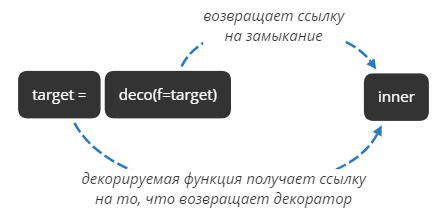
\includegraphics[scale=0.85]{figures/target_deco_formula.png}
	\caption{ К вопросу о механизме работы декоратора с вложенной функцией }\label{fig:target_deco_formula}
\end{figure}



\subsection{Написание декораторов класса}

Есть возможность реализовать декораторы класса, правда, они используются гораздо реже. Декораторы класса работают так же, как и декораторы функций, но с классами. Следующий фрагмент кода -- это пример декоратора класса, который устанавливает атрибуты для двух классов
\begin{lstlisting}[
style = ironpython,
numbers = none	
]
import uuid

def set_class_name_add_id(klass):
    klass.name = str(klass)        # станет атрибутом класса
    klass.random_id = uuid.uuid4() # станет атрибутом класса
    return klass
    
@set_class_name_and_id
class SomeClass:
    pass
\end{lstlisting}

Когда класс будет объявлен и загружен, он установит атрибуты класса \texttt{name} и \texttt{random\_id}
\begin{lstlisting}[
style = ironpython,
numbers = none	
]
>>> SomeClass.name # <class '__main__.SomeClass'>
>>> SomeClass.random_id # UUID('9b75e122-f52a-468b-9796-311d394de2bf')
\end{lstlisting}

Еще можно таким способом регистрировать объявленные классы
\begin{lstlisting}[
style = ironpython,
numbers = none	
]
import numpy as np


registry = {}


def register_class(cl):
    name = str(cl.__name__)
    random_id = np.random.randn()
    registry[name] = random_id
    return cl # возвращает ссылку на класс


@register_class
class TestClass:
    pass


@register_class
class SimpleClass:
    pass


for key, value in registry.items():
    print(key, value)
\end{lstlisting}

Иногда бывает удобно применять декораторы класса для декорирования функций или других классов
\begin{lstlisting}[
style = ironpython,
numbers = none	
]
class CountClass:
    def __init__(self, f):
        self.f = f
        self.called = 0
        
    
    def __call__(self, *args, **kwargs):
        self.called += 1
        return self.f(*args, **kwargs)
        
        
@CountClass
def print_hello():
    print("hello")   
    

print(print_hello.called) # 0
print_hello()
print(print_hello.called) # 1
print_hello()
print(print_hello.called) # 2
\end{lstlisting}

Здесь при загрузке модуля аргумент \texttt{f} метода \verb|__init__()| получает ссылку на декорируемую функцию, а переменная \texttt{self.called} инициализируется нулем.

Теперь при каждом вызове функции \texttt{print\_hello()} будет вызываться метод \verb|__call__()|. При этом значение переменной \texttt{self.called} будет увеличиваться на единицу, а затем будет вызываться собственно задекорированная функция.

\section{Методы в Python}

\subsection{Статические методы}

\emph{Статические методы} принадлежат классу, а не его экземпляру, поэтому они фактически не работают и не влияют на экземпляры класса. Вместо этого статический метод оперирует параметрами, которые принимает. Статические методы обычно используются для создания функций полезности, потому что не зависят от состояния классов или объектов.

Использование статических методов предоставляет несколько преимуществ:
\begin{itemize}
	\item Скорость. Python не должен устанавливать связанный метод для каждого связанного объекта. Связанный метод -- это тоже объект, а создание нового объекта отнимает системные ресурсы, хоть и незначительные,
	
	\item Удобочитаемость кода. Видя декоратор \verb|@staticmethod|, мы знаем, что метод не зависит от состояния объекта.
\end{itemize}

К сожалению, Python не всегда способен определить, является ил метод статическим, -- это издержки дизайна языка.

\subsection{Классовые методы}

Классовые методы связаны с классом, а не с экземпляром. Классовые методы очень полезны при динамическом создании экземпляров класса
\begin{lstlisting}[
style = ironpython,
numbers = none	
]
class Pizza:
    def __init__(self, ingredients):
        self.ingredients = ingredients
        
    @classmethod
    def from_fridge(cls, fridge):
        return cls(fridge.get_cheese() + fridge._get_vegetables())
\end{lstlisting}


\section{Замыкания/фабричные функции в \texttt{Python}}

Под термином \emph{замыкание} или \emph{фабричная функция} подразумевается объект функции, который сохраняет значения в \emph{объемлющих областях видимости}, даже когда эти области могут прекратить свое существование \cite[\strbook{488}]{lutz:learningpython-2011}.

В источнике \cite[\strbook{222}]{ramalho:python-2016} приводится несколько отличное определение\footnote{Определение содержит авторские правки}: \emph{замыкание} -- это вложенная функция с расширенной областью видимости, которая охватывает все \emph{неглобальные} переменные, объявленные в области видимости объемлющей функции, и способная работать с этими переменными даже после того как локальная область видимости объемлющей функции будет уничтожена.

Замыкания и вложенные функции особенно удобны, когда требуется реализовать концепцию отложенных вычислений \cite{beazley:python-2010}.

\remark{
Все же правильнее <<фабрикой функций>> называть всю конструкцию из объемлющей и вложенной функций, а <<замыканием>> -- только вложенную функцию
}

Рассмотрим в качестве примера следующую функцию

\begin{lstlisting}[
style = ironpython,
emph = {maker, action},
numbers = none
]
def maker(N):
    def action(X):
        return X**N  # функция action запоминает значение N в объемлющей области видимости
    return action
\end{lstlisting}

Здесь определяется внешняя функция, которая просто создает и возвращает вложенную функцию, не вызывая ее. Если вызвать внешнюю функцию

\begin{lstlisting}[
style = ironpython,
emph = {maker},
numbers = none
]
>>> f = maker(2)  # запишет 2 в N
>>> f  # <function action at 0x0147280>
\end{lstlisting}
она вернет ссылку на созданную ею вложенную функцию, созданную при выполнении вложенной инструкции \texttt{def}. Если теперь вызвать то, что было получено от внешней функции

\begin{lstlisting}[
style = ironpython,
numbers = none
]
>>> f(3)  # запишет 3 в X, в N по-прежнему хранится число 2
>>> f(4)  # 4**2
\end{lstlisting}
будет вызвана вложенная функция, с именем \texttt{action} внутри функции \texttt{maker}. Самое необычное здесь то, что вложенная функция продолжает хранить число 2, значение переменной \texttt{N} в функции \texttt{maker} даже при том, что к моменту вызова функции \texttt{action} функция \texttt{maker} уже \emph{завершила свою работу и вернула управление}.

Когда функция используется как вложенная, в замыкание включается все ее окружение, необходимое для работы внутренней функции \cite[\strbook{137}]{beazley:python-2010}.

\subsection{Области видимости и значения по умолчанию применительно к переменным цикла}

Существует одна известная особенность для функций или lambda-выражений: если lambda-выражение или инструкция \texttt{def} вложены в цикл внутри другой функции и вложенная функция ссылается на переменную из объемлющей области видимости, которая изменяется в цикле, все функции, созданные в этом цикле, будут иметь одно и то же значение -- значение, которое имела переменная на последней итерации \cite[\strbook{492}]{lutz:learningpython-2011}.

Например, ниже предпринята попытка создать список функций, каждая из которых запоминает текущее значение переменной \texttt{i} из объемлющей области видимости

\begin{lstlisting}[
title = {\sffamily Эта реализация работать НЕ будет},
style = ironpython,
emph = {makeActions},
numbers = none
]
def makeActions():
    acts = []
    for i in range(5):  # область видимости объемлющей функции
        acts.append(
            lambda x: i**x  # локальная область видимости вложенной анонимной функции
        ) 
    return acts
    
acts = makeActions()
print(acts[0](2))  # вернет 4**2, последнее значение i
print(acts[3](2))  # вернет 4**2, последнее значение i
\end{lstlisting}

Такой подход не дает желаемого результата, потому что поиск переменной в объемлющей области видимости производится позднее, \emph{при вызове вложенных функций}, в результате все они получат одно и то же значение (значение, которое имела переменная цикла на последней итерации).

Это один из случаев, когда необходимо явно сохранять значение из объемлющей области видимости в виде аргумента со значением по умолчанию вместо использования ссылки на переменную из объемлющей области видимости.

То есть, чтобы фрагмент заработал, необходимо передать текущее значение переменной из объемлющей области видимости в виде значения по умолчанию. Значения по умолчанию вычисляются в момент \emph{создания вложенной функции} (а не когда она \emph{вызывается}), поэтому каждая из них сохранит свое собственное значение \texttt{i}

\begin{lstlisting}[
title = {\sffamily Правильная реализация},
style = ironpython,
emph = {makeActions},
numbers = none
]
def makeActions():
    acts = []
    for i in range(5):
        acts.append(
            lambda x, i=i: i**x  # сохранить текущее значение i
        )
    return acts

acts = makeActions()
print(acts[0](2))  # вернет 0**2
print(acts[2](2))  # вернет 2**2
\end{lstlisting}

\quinta{%
Значения аргументов по умолчанию вложенных функций, динамически создаваемых в цикле на уровне области видимости объемлющей функции, вычисляются в момент \emph{создания} этих вложенных функций, а не в момент их вызова, поэтому \texttt{lambda x, i=i: ...} работает корректно
}

\section{Значения по умолчанию изменяемого типа данных в \texttt{Python}}

Если у функции есть аргумент, который получает ссылку на \emph{объект изменяемого типа данных} как на значение по умолчанию, то \emph{все вызовы функций} будут ссылаться на один и тот же изменяемый объект\footnote{По этой причине, как правило, только \emph{объекты неизменяемого типа данных} могут быть значениями по умолчанию. Если значение аргумента функции должно иметь возможность изменяться динамически, то этот аргумент функции инициализируют с помощью \texttt{None}, а затем передают ссылку на объект по условию} (идентификационный номер объекта не изменится).

Это удивляет. И когда говорят об аномальном поведении функции, аргумент которой ссылается на объект изменяемого типа данных, то обычно такое поведение объясняют следующим образом: значения аргументов по умолчанию вычисляются только один раз при загрузке модуля \cite[\strbook{77}]{slatkin:python-2016}. Однако такое объяснение не вскрывает механизм <<разделения>> ссылки между вызовами.

Лучше сказать так: если у функции есть аргумент, который ссылается на объект изменяемого типа данных, и в теле функции выполняется какая-то работа с этим изменяемым объектом (т.е. вносятся изменения в объект), то новые вызовы такой функции не сбрасывают значения по умолчанию до тех, которые были вычислены при загрузке модуля. Другими словами, если аргумент функции ссылается на объект изменяемого типа данных и над этим объектом выполняется какая-то работа в теле функции, то каждый новый вызов функции будет изменять этот изменяемый объект в \emph{определении} функции и потому каждый следующий вызов будет оперировать с уже измененным объектом изменяемого типа данных.

\remark{
Значения аргументов по умолчанию для избежания странного поведения функции должны ссылаться на \emph{объекты неизменяемого типа данных}
}

\section{Генераторы, сопрограммы в \texttt{Python}}

Цепочки вычислений лучше строить на базе генераторов или сопрограмм. Например простую цепочку преобразований можно построить и с помощью функции \texttt{reduce} (но лучше так не делать!)
\begin{lstlisting}[
style = ironpython,
title = {\sffamily Так лучше не делать!},
numbers = none	
]
from functools import reduce

test_str = 'python fortran matlab'
pipe_func = (
    str.split,  # разбивает переданную строку по пробелу и возвращает список
    lambda lst: (elem.upper() for elem in lst)  # каждую выделенную на предыдущем этапе
                                                # строку приводит к верхнему регистру
)

main_red = reduce(
    lambda args, f: f(args),
    pipe_func,
    test_str
)

for elem in main_red:
    print(elem)
# PYTHON
# FORTRAN
# MATLAB
\end{lstlisting}

Для данной задачи конвейер преобразований на базе генераторов может выглядеть так
\begin{lstlisting}[
style = ironpython,
title = {\sffamily Правильный вариант решения задачи о конвейерах преобразований},
numbers = none	
]
def gen_split(s: str):
    '''
    Функция-генератор
    '''
    for elem in s.split():
        yield elem
        
def gen_upper(sub_str: str):
    '''
    Функция-генератор
    '''
    for elem in sub_str:
        yield elem.upper()
        
main_gen = gen_upper(gen_split(test_str))  # объект-генератор
for elem in main_gen:
    print(elem)
# PYTHON
# FORTRAN
# MATLAB
\end{lstlisting}

\section{Библиотека \texttt{functools}}



\subsection{Каррированные функции с помощью \texttt{functools.partial}}

\begin{lstlisting}[
style = ironpython,
numbers = none	
]
from functools import partial

# инициализируем частичную функцию списком
part_f = partial(lambda lst, transform: [transform(elem) for elem in lst],
                 lst=['python', 'fortran'])
# передает преобразование
part_f(transform=str.upper)  # ['PYTHON', 'FORTRAN']
\end{lstlisting}

Иногда бывает удобно использовать метод \texttt{partialmethod}
\begin{lstlisting}[
style = ironpython,
emph = {__init__, set_live, get_live, __call__},
numbers = none	
]
from functools import partialmethod

class Live:
    def __init__(self):
        self._live = False
        
    def set_live(self, state: bool):
        self._live = state
        
    def get_live(self):
        return self._live
        
    def __call__(self):
        return self.get_live()
    
    # атрибуты класса    
    set_alive = partialmethod(set_live, True) # замораживает метод set_live() со значением True
    set_dead = partialmethod(set_live, False) # замораживает метод set_live() со значением False
    
live = Live()
live.set_alive()  # изменит значение атрибута self._live на True
                  # метод set_alive() вызовет метод set_live(True)
print(live())  # True: вызовет __call__, а тот в свою очередь get_live()
# разумеется можно вызвать метод set_live(False) и напрямую
\end{lstlisting}



\section{Калибровка классификаторов}

Подробности в статье А. Дьяконова \href{https://dyakonov.org/2020/03/27/%D0%BF%D1%80%D0%BE%D0%B1%D0%BB%D0%B5%D0%BC%D0%B0-%D0%BA%D0%B0%D0%BB%D0%B8%D0%B1%D1%80%D0%BE%D0%B2%D0%BA%D0%B8-%D1%83%D0%B2%D0%B5%D1%80%D0%B5%D0%BD%D0%BD%D0%BE%D1%81%D1%82%D0%B8/}{<<Проблема калибровки уверенности>>}.
\vspace{2mm}

Ниже описываются способы оценить качество калибровки алгоритма. Надо сравнить \emph{уверенность} (confidence) и \emph{долю верных ответов} (accuracy) на тестовой выборке.

Если классификатор <<хорошо откалиброван>> и для большой группы объектов этот классификатор возвращает вероятность принадлежности к положительному классу 0.8, то среди этих объектов будет приблизительно 80\% объектов, которые в действительности принадлежат положительному классу. То есть, если для группы точек данных общим числом 100 классификатор возвращает вероятность положительного класса 0.8, то приблизительно 80 точек на самом деле будут принадлежать положительному классу и доля верных ответов тогда составит 0.8.

\subsection{Непараметрический метод гистограммной калибровки (Histogram Binning)}

Изначально в методе использовались бины одинаковой ширины, но можно использовать и равномощные бины.

Недостатки подхода:

\begin{itemize}
	\item число бинов задается наперед,
	
	\item функция деформации не непрерывна,
	
	\item в <<равноширинном варианте>> в некоторых бинах может содержаться недостаточное число точек.
\end{itemize}

Метод был предложен Zadrozny В. и Elkan C. \href{http://cseweb.ucsd.edu/~elkan/calibrated.pdf}{\ttfamily Obtaining  calibrated  probability  estimates  from  decision  trees  and naive bayesian classifiers}.

\subsection{Непараметрический метод изотонической регрессии (Isotonic Regression)}

Строится монотонно неубывающая функция деформации оценок алгоритма.

Метод был предложен Zadrozny B. и Elkan C. \href{http://citeseerx.ist.psu.edu/viewdoc/download?doi=10.1.1.13.7457&rep=rep1&type=pdf}{\ttfamily Transforming classifier scores into accurate multiclass probability estimates}.

Функция деформации по-прежнему не является непрерывной.

\subsection{Параметрическая калибровка Платта (Platt calibration)}

Изначально этот метод калибровки разрабатывался только для метода опорных векторов, оценки которого лежат на вещественной оси (по сути, это расстояния до оптимальной разделяющей классы прямой, взятые с нужным знаком). Считается, что этот метод не очень подходит для других моделей.

Предложен Platt~J. \href{http://citeseerx.ist.psu.edu/viewdoc/download;jsessionid=EA4888FEE74FB677B492740F59CDFE1F?doi=10.1.1.41.1639&rep=rep1&type=pdf}{\ttfamily Probabilistic  outputs  for  support  vector machines and comparisons to regularized likelihood methods}.

\subsection{Логистическая регрессия в пространстве логитов}

\subsection{Деревья калибровки}

Стандартный алгоритм строит строит суперпозицию дерева решений на исходных признаках и логистических регрессий (каждая в своем листе) над оценками алгоритма:

\begin{itemize}
	\item Построить на исходных признаках решающее дерево (не очень глубокое),
	
	\item В каждом листе -- обучить логистическую регрессию на одном признаке,
	
	\item Подрезать дерево, минимизируя ошибку.
\end{itemize}

\subsection{Температурное шкалирование (Temperature Scaling)}

Этот метод относится к классу DL-методов калибровки, так как он был разработан именно для калибровки нейронных сетей. Метод представляет собой простое многомерное обобщение шкалирования Платта.

\section{Приемы работы с менеджером пакетов \texttt{conda}}

\subsection{Создание виртуального окружения}

Создать виртуальное окружение \texttt{dashenv}

\begin{lstlisting}[
numbers = none
]
conda create --name dashenv
\end{lstlisting}

Создать виртуальное окружение с указанием версии \texttt{Python}

\begin{lstlisting}[
numbers = none
]
conda create --name testenv python=3.6
\end{lstlisting}

Создать виртуальное окружение с указанием пакета

\begin{lstlisting}[
numbers = none
]
conda create --name testenv scipy
\end{lstlisting}

Создать виртуальное окружение с указанием версии \texttt{Python} и нескольких пакетов

\begin{lstlisting}[
numbers = none
]
conda create --name testenv python=3.6 scipy=0.15.0 astroid babel
\end{lstlisting}

\remark{%
Рекомендуется устанавливать сразу несколько пакетов, чтобы избежать конфликта зависимостей
}

Для того чтобы при создании нового виртуального окружения не требовалось каждый раз устанавливать базовые пакеты, которые обычно используются в работе, можно привести их список в конфигурационном файле \texttt{.condarc} в разделе \texttt{create\_default\_packages}

\begin{lstlisting}[
title = {\sffamily .condarc},
numbers = none
]
ssl_verify: true
channels:
 - conda-forge
 - defaults
report_errors: true
default_python:
create_default_packages:
 - matplotlib
 - numpy
 - scipy
 - pandas
 - seaborn
\end{lstlisting}

Если для текущего виртуального окружения не требуется устанавливать пакеты из набора по умолчанию, то при создании виртуального окружения следует указать специальный флаг
\lstinline{--no-default-packages}

\begin{lstlisting}[
numbers = none
]
conda create --no-default-packages --name testenv python
\end{lstlisting}

Создать виртуальное окружение можно и из файла \texttt{environment.yml} (первая строка этого файла станет именем виртуального окружения)

\begin{lstlisting}[
title = {\sffamily environment.yml},
numbers = none
]
name: stats2
channels:
 - conda-forge
 - defaults
dependencies:
 - python=3.6   # or 2.7
 - bokeh=0.9.2
 - numpy=1.9.*
 - nodejs=0.10.*
 - flask
 - pip:
  - Flask-Testing
\end{lstlisting}

\begin{lstlisting}[
numbers = none
]
conda env create -f environment.yml
\end{lstlisting}

При создании виртуального окружения можно указать путь до целевой директории, где будут размещаться файлы окружения. Следующая команда создаст виртуальное окружение в поддиректории текущей рабочей директории \texttt{envs}\footnote{В данном случае чтобы удалить виртуальную среду достачно просто удалить директорию \texttt{envs}}

\begin{lstlisting}[
numbers = none
]
conda create --prefix ./envs jupyterlab matplotlib
\end{lstlisting}

С помощью файла спецификации можно создать \emph{идентичное виртуальное окружение} (i) на той же платформе операционной системы, (ii) на той же машине, (iii) на какой-либо другой машине (перенести настройки окружения).

Для этого предварительно требуется создать собственно файл спецификации

\begin{lstlisting}[
numbers = none
]
conda list --explicit > spec-file.txt
\end{lstlisting}

Имя файла спецификации может быть любым. Файл спецификации обычно не является кросс-платформенным и поэтому имеет комментарий в верхней части файла (\lstinline{#platform: osx-64}), указывающий платформу, на которой он был создан.

Теперь для того чтобы \emph{создать} окружение достаточно воспользоваться командой

\begin{lstlisting}[
numbers = none
]
conda create --name myenv --file spec-file.txt
\end{lstlisting}

Файл спецификации можно использовать для установки пакетов в существующее окружение

\begin{lstlisting}[
numbers = none
]
conda install --name myenv --file spec-file.txt
\end{lstlisting}


\subsection{Активация/деактивация виртуального окружения}

Активировать виртуальное окружение \texttt{dashenv}

\begin{lstlisting}[
numbers = none
]
conda activate dashenv
\end{lstlisting}

Активировать виртуальное окружение в случае, когда оно создавалось с \lstinline{--prefix}, можно указав полный путь до окружения
\begin{lstlisting}[
numbers = none
]
conda activate E:\[WorkDirectory]\[Python_projects]\directory_for_experiments\envs
\end{lstlisting}

В этом случае в строке приглашения командной оболочки по умолчанию будет отображаться полный путь до окружения. Чтобы заменить длинный префикс в имени окружения на более удобный псевдоним достаточно использовать конструкцию

\begin{lstlisting}[
numbers = none
]
conda config --set env_prompt ({name})
\end{lstlisting}
которая добавит в конфигурационный файл \texttt{.condarc} следующую строку

\begin{lstlisting}[
title = {\sffamily .condarc},
numbers = none
]
...
env_prompt: ({name})
\end{lstlisting}
и теперь имя окружения будет \texttt{(envs)}.

Деактивировать виртуальное окружение

\begin{lstlisting}[
numbers = none
]
conda deactivate
\end{lstlisting}

\subsection{Обновление виртуального окружения}

Обновить виртуальное окружение может потребоваться в следующих случаях:

\begin{itemize}
	\item обновилась одна из ключевых зависимостей,
	
	\item требуется добавить пакет (добавление зависимости),
	
	\item требуется добавить один пакет и удалить другой.
\end{itemize}

В любом из этих случаев все что нужно для того чтобы обновить виртуальное окружение это просто обновить файл \texttt{environment.yml}\footnote{Этот файл должен находится в той же директории что и директория окружения \texttt{envs}}, а затем запустить команду

\begin{lstlisting}[
numbers = none
]
conda env update --prefix ./envs --file environment.yml --prune
\end{lstlisting}

Опция \lstinline{--prune} приводит к тому, что \texttt{conda} удаляет все зависимости, которые больше не нужны для окружения.

\subsection{Вывод информации о виртуальном окружении}

Вывести список доступных виртуальных окружений

\begin{lstlisting}[
numbers = none
]
conda env list
\end{lstlisting}

Вывести список пакетов, установленных в указанном окружении

\begin{lstlisting}[
numbers = none
]
conda list --name myenv
\end{lstlisting}

Вывести информацию по конкретному пакету указанного окружения

\begin{lstlisting}[
numbers = none
]
conda list --name dashenv matplotlib
\end{lstlisting}


\subsection{Удаление виртуального окружения}

Удалить виртуальное окружение \texttt{heroku\_env}

\begin{lstlisting}[
numbers = none
]
conda env remove --name heroku_env
\end{lstlisting}

\subsection{Экспорт виртуального окружения в \texttt{environment.yml}}

Экспортировать активное виртуальное окружение в yml-файл

\begin{lstlisting}[
numbers = none
]
conda env export > environment.yml
\end{lstlisting}


\section{Инструмент автоматического построения дерева проекта под задачи машинного обучения}

Для автоматизации построения типового (или кастомизированного) дерева проекта по машинному обучению и анализу данных удобно использовать \href{https://cookiecutter.readthedocs.io/en/1.7.2/README.html}{\texttt{cookicutter}}.

На операционную систему под управлением \texttt{Windows} \texttt{cookicutter} можно установить с помощью менеджера пакетов \texttt{pip}

\begin{lstlisting}[
numbers = none
]
pip install cookiecutter
\end{lstlisting} 
а на операционную систему под управлением \texttt{MacOS X} с помощью менеджера \texttt{brew}

\begin{lstlisting}[
numbers = none
]
brew install cookiecutter
\end{lstlisting}

В самом простом случае \texttt{cookicutter} можно использовать как утилиту командной строки. Например для того чтобы создать проект по шаблону для задач машинного обучения достаточно сделать следующее

\begin{lstlisting}[
style = ironpython,
numbers = none,
]
cookiecutter https://github.com/drivendata/cookiecutter-data-science
\end{lstlisting}

Утилита предложит ответить на несколько вопросов (название репозитория, имя автора и т.д.), а затем создаст дерево проекта.

\section{Управление локальными переменными окружения проекта}

Для того чтобы создать \emph{локальные переменные проекта}\footnote{То есть переменные, привязанные к текущему проекту} достаточно разместить пары вида <<ключ=значение>> в файле \texttt{.env}, а затем прочитать его с помощью специальной библиотеки \texttt{dotenv} \url{https://pypi.org/project/python-dotenv/}. Например

\begin{lstlisting}[
style = ironpython,
numbers = none
]
#.env в текущей директории проекта
EMAIL = leor.finkelberg@yandex.ru
POSTGRESQL_PASSWORD = Evdimonia
\end{lstlisting}

\begin{lstlisting}[
style = ironpython,
numbers = none
]
import os
from pathlib import Path
from dotenv import load_dotenv

dotenv_path = Path(__file__).resolve().parents[0].joinpath('.env')
print(f'[INFO] path: {dotenv_path}')  # [INFO] path: E:\[WorkDirectory]\[Python_projects]\directory_for_experiments\.env

load_dotenv(dotenv_path)  # загрузить .env

# извлекать значения локальных переменных окружения проекта можно с помощью `os.getenv(key)`
# или `os.environ.get(key)`
for key in (s.upper() for s in ('email', 'postgresql_password')):
    print('[INFO] from file `.env`({}) -> {}'.format(key, os.getenv(key)))
\end{lstlisting}

\section{Приемы работы с модулем \texttt{subprocess}}

Ниже приводится пример использования модуля \texttt{subprocess} для отыскания самого большого файла в \texttt{git}-репозитории
\begin{lstlisting}[
style = ironpython,
emph = {popen_2_str},
numbers = none
]
import os
import subprocess
import pathlib
from subprocess import Popen, PIPE, STDOUT

# --- объявление функций: begin
def popen_2_str(cmd: str, shell=True, universal_newlines=True, stdout=PIPE) -> str:
    return Popen(cmd, shell=shell,
                 universal_newlines=universal_newlines,
                 stdout=stdout).stdout.read().strip()

def stat(filename):
    res = popen_2_str(f"stat {filename}")
    print(f'>>> Statistic:\n{res}')

def summary(commits):
    print(f'### Summary ({__file__}) ###:\n>>> idx-file name: {idx_file}'
          f'\n>>> SHA blob: {shablob}\n>>> Commits:')
    print(commits)
# --- объявление функций: end

GIT_PATH = pathlib.Path('.git/objects/pack/')

# тоже самое что и `git gc &> /dev/null`
exit_code = subprocess.call("git gc", shell=True,
                            stdout=open(os.devnull, 'w'), stderr=STDOUT)

if not exit_code:
    # возвращает имя idx-файла
    idx_file = popen_2_str(f"ls -l {GIT_PATH} | grep -iE '*.idx' "
                           f"| awk -F ' ' '{{ print $9 }}'")
    # возвращает абсолютный путь до idx-файла
    abs_path_idx_file = pathlib.Path.joinpath(GIT_PATH, idx_file)
    if os.path.exists(abs_path_idx_file):
    # возвращает SHA <<большого>> файла
        shablob = popen_2_str(f"git verify-pack -v {abs_path_idx_file} | sort -k 3 -n "
                              f"| tail -n 1 | awk -F ' ' '{{ print $1 }}'")
        # возвращает имя файла по его SHA
        filename = popen_2_str(f"git rev-list --objects --all | grep {shablob} "
                               f"| awk -F ' ' '{{ print $2 }}'")
        # возвращает коммиты, связанные с данным файлом
        commits = popen_2_str(f"git log --oneline -- {filename}")
        summary(commits)
        stat(filename)
    else:
        print(f"File {abs_path_idx_file} not found...")
else:
    print('Something went wrong.')
\end{lstlisting}

\section{Решающие деревья и сопряженные вопросы}

\subsection{Коэффициент Джини}

\emph{Коэффициент Джини}\footnote{Еще говорят индекс Джини или загрязненность Джини} (Gini impurity) это просто вероятность неверной маркировки в узле случайно выбранного образца (для чистых листьев коэффициент Джини равен 0)
\begin{align}
	I_G(n) = 1 - \sum_{i=1}^{J}p_i^2,
\end{align}
где $ p_i $ -- частоты представителей разных классов в листе дерева.

К примеру, если решается задача бинарной классификации ($ J = 2 $) на выборке из 6 объектов и в данном расщеплении в один класс попали 2 объекта, а в другой 4, то индекс Джини будет равен
\begin{align}
	I_G(n)=1 - \left( \left( \frac{2}{6} \right)^2 + \left( \frac{4}{6} \right)^2 \right) = 0,444.
\end{align}

\subsection{Случайный лес}

Случайный лес -- это модель, представляющая ансамбль решающих деревьев, дополненная двумя концепциями:
\begin{itemize}
	\item концепцией бутрстапированных выборок,
	
	\item концепцией случайных подпространств.
\end{itemize}

Хотя каждое решающее дерево может иметь большой разброс по отношению к определенному набору тренировочных данных, обучение деревьев на разных наборах образцов позволяет снизить общий разброс леса.


\section{Анализ временных рядов}

\subsection{Признаки на временных рядах}

Можно выделить следующие несколько групп признаков на временных рядах:
\begin{itemize}
	\item признаки на основе коэффициентов автокорреляции и частных коэффицентов автокорреляции,
	
	\item оптимальное значение параметра $ \lambda $ преобразования Бокса-Кокса,
	
	\item коэффициент Херста,
	
	\item количество раз, когда временной ряд пересекает свою собственную медиану,
	
	\item признаки, рассчитываемые на основе STL-компонент разложения временного ряда,
	
	\item дисперсия дисперсии, рассчитанных по наблюдениям из непересекающихся временных отрезков,
	
	\item дивергенция Кульбака-Лейблера в следующих друг за другом отрезках,
	
	\item спектральная энтропия ряда,
	
	\item дисперсия средних значений,
	
	\item минимальное число дифференциирований временного ряда, необходимое для достижения его стационарности.
\end{itemize}


\subsection{Кросс-валидация на временных рядах}

\subsubsection{Авторская методика подбора гиперпараметров модели на кросс-валидации}

Алгоритм \pic{fig:cv_time_ser}:
\begin{itemize}
	\item Весь набор данных (весь временной ряд) разбивается, как обычно, на \emph{обучающее} и \emph{тестовое} подмноженство данных,
	
	\item Обучающий набор данных разбивается на несколько блоков (например, на 3 блока),
	
	\item Каждый блок обучающего набора данных разбивается на несколько подблоков,
	
	\item На каждом подблоке, для каждой комбинации гиперпараметров вычисляется ошибка на валидационном подмножестве следующим образом: обучаемся на блоке 1-1, тестируемся на блоке 1-2, затем обучаемся на блоках 1-1 и 1-2, тестируемся на блоке 1-3 и т.д. Промежуточные оценки, вычисленные сначала на блоке 1-2, затем на блоке 1-3 и т.д. нужны для получения представляения о динамике изменения валидационной ошибки по мере увеличения объема обучающего набора данных. То есть фиксируем комбинацию гиперпараметров (сейчас для простоты пропустим этап промежуточных вычислений валидационных ошибок) и вычисляем ошибку для этой комбинации на валидационном блоке 1-3. Получаем ошибку для блока 1 и первой комбинации гиперпараметров (обозначим ее $ E_{1}^{(1)} $). Затем получаем ошибку для блока 1 и второй комбинации гиперпараметров, т.е. $ E_{1}^{(2)} $ и так для остальных комбинаций гиперпараметров. В итоге получается первая строка таблицы <<разбиения -- комбинации>>. Повторяем процедуру для других блоков и получаем следующие строки таблицы <<разбиения -- комбинации>>
	\begin{table}[h]
		\centering
		\caption{\itshape Разбиения и комбинации}\label{tab:splits_and_comb}
		%\renewcommand{\arraystretch}{1.05}
		\begin{tabular}{lllll}
		    {} & {Комбинация 1} & {Комбинация 2} & $ \ldots $ & {Комбинация $ n $} \\
			{Блок 1} & $ E_{1}^{(1)} $ & $ E_{1}^{(2)} $ & $ \ldots $ & $ E_{1}^{(n)} $ \\
			{Блок 2} & $ E_{2}^{(1)} $ & $ E_{2}^{(2)} $ & $ \ldots $ & $ E_{2}^{(n)} $ \\
			{Блок 3} & $ E_{3}^{(1)} $ & $ E_{3}^{(2)} $ & $ \ldots $ & $ E_{3}^{(n)} $
		\end{tabular}
	\end{table}
	
	
	\item Затем усредняем ошибку по блокам и получаем среднюю эффективность для $ i $-комбинации гиперпараметров, т.е. $ \vec{E}^{(i)} $,
	
	\item Выбираем ту комбинацию гиперпараметров, которая отвечает наименьшей средней оценке $ \vec{E}^{(i)} $,
	
	\item Переобучаем модель еще раз на этой наиболее эффективной комбинации гиперпараметров, но уже на всем обучающем наборе данных,
	
	\item Оцениваем обобщающую способность модели на тестовом наборе данных.
\end{itemize}

\begin{figure}[h]
	\centering
	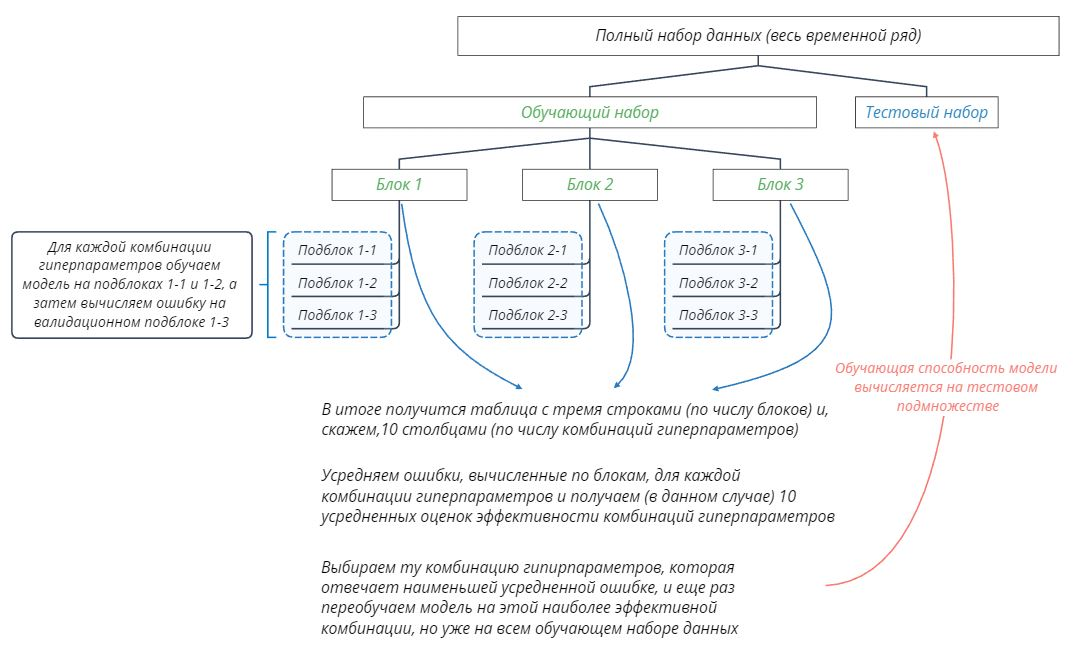
\includegraphics[scale=0.8]{figures/cross-val-time-series.jpg}
	\caption{ Подбор гиперпараметров на цикле кросс-валидации и оценка обобщающей способности модели на тестовом наборе данных }\label{fig:cv_time_ser}
\end{figure}

\subsection{Кросс-валидация на временных рядах по мотивам статьи Time Series Nested Cross-Validation}

Оригинал статьи: \href{https://towardsdatascience.com/time-series-nested-cross-validation-76adba623eb9}{Time Series Nested Cross-Validation}.

В случае обычной $ k $-блочной перекрестной проверки мы имеющийся набор данных разбиваем на обучающий и тестовый. А затем обучающий разбиваем на подобучающий и валидационный. На подобучающем наборе данных мы обучаем модель, на валидационном настраиваем гиперпараметры. Затем модель обучается на полном обучающем наборе данных с использованием лучшей комбинации параметров. На тестовом наборе данных определяется обобщающая способность модели (\pic{fig:cv_classic}).

\begin{figure}[h]
	\centering
	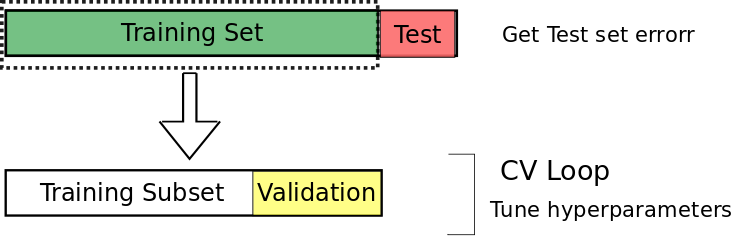
\includegraphics[scale=0.35]{figures/cv_classic.png}
	\caption{ Стандартная процедура кросс-валидации }\label{fig:cv_classic}
\end{figure}

На временных рядах традиционная перекрестная проверка не должна использоваться, так как возможна утечка данных из <<будущего>>. Рекомендуется использовать \emph{вложенную перекрестную проверку} (nested cross-validation). Вложенная перекрестная проверка включает внешний цикл для вычисления ошибок и внутренний цикл для подбора параметров. 

Внутренний цикл работает как и раньше: обучающий набор данных разбивается на подобучающий набор и валидационный набор. Модель обучается на подобучающем наборе, а на валидационном наборе подбираются параметры. А во внешнем цикле исходный набор данных (временной ряд) разбивается на обучающий и тестовый наборы данных, и ошибка каждого разбиения усредняется (\pic{fig:nested_cv}).

\begin{figure}[h]
	\centering
	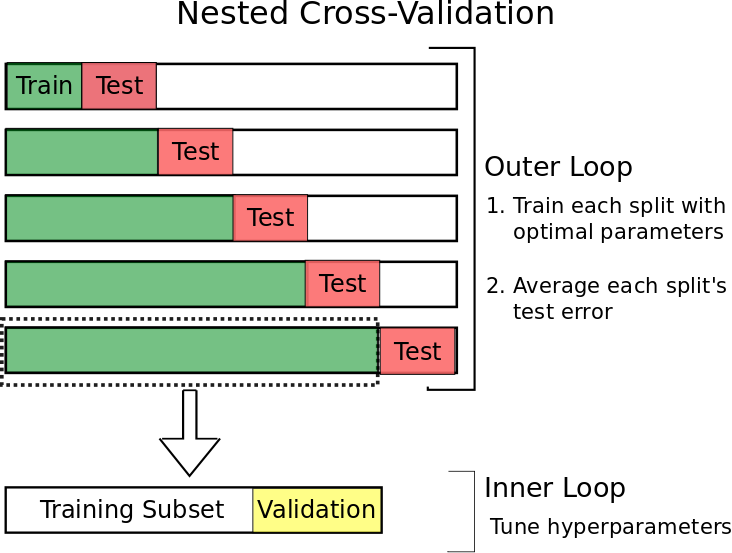
\includegraphics[scale=0.35]{figures/nested_cv.png}
	\caption{ Вложенная перекресная проверка на временном ряде }\label{fig:nested_cv}
\end{figure}

Вложенная перекрестная проверка (чуть подробнее):
\begin{itemize}
	\item Весь временной ряд разбиваем на несколько блоков,
	
	\item Первый блок разбивается на \emph{обучающий} и \emph{тестовый} набор данных,
	
	\item Обучающий набор данных первого сплита разбивается на \emph{подобучающий} и \emph{валидационный} набор данных,
	
	\item Для каждой комбинации гиперпараметров обучаем модель на \emph{подобучающем} наборе данных, а затем вычисляем метрку качества на валидационном наборе данных (первого сплита),
	
	\item Выбираем такую комбинацию гиперпараметров, которая отвечает наибольшему значению метрики качества (или наименьшому значению ошибки), и обучаем модель еще раз с наилучшей комбинацией параметров, но уже на всем обучающем наборе данных первого сплита,
	
	\item Вычисляем метрику качества (или ошибку) на тестовом наборе данных первого сплита,
	
	\item Переходим к следующему блоку и повторяем всю цепочку.
	
	\item В итоге полученные ошибки тестового набора данных на каждом разбиении усредняем по этим разбиениям.
\end{itemize}


\subsection{Синус-косинусное кодирование во временных рядах}

Признаки типа <<день недели>>, <<время суток>>, <<день месяца>> и пр., строго говоря, имеют циклическую природу и игнорировать ее нельзя. Таким образом, обычно рекомендуется признаки, имеющие отношение к временной шкале кодировать с помощью синус-косинусного преобразовании
\begin{align*}
	\tilde{f}_i^{(s)} = \sin (f_i \cdot \dfrac{2 \pi}{n_i}),\ \tilde{f}_i^{(c)} = \cos (f_i \cdot \dfrac{2 \pi}{n_i}),
\end{align*}
где $ f_i $ -- $ i $-ый признак; $ \tilde{f}_i^{(s)}, \tilde{f}_i^{(c)} $ -- новое закодированное значение $ i $-ого признака для синуса и косинуса соответственно; $ n_i $ -- число уникальных значений признака (например, для времени суток это 24, для дней недели это 7 и т.д.).

Пример
\begin{lstlisting}[
style = ironpython,
numbers = none	
]
df["hr_sin"] = np.sin(df["hr"]*2*np.pi/24)
df["hr_cos"] = np.cos(df["hr"]*2*np.pi/24)

df["mnth_sin"] = np.sin((df["mnth"] - 1)*2*np.pi/12)
df["mnth_cos"] = np.cos((df["mnth"] - 1)*2*np.pi/12)
\end{lstlisting}


\subsection{Прогнозирование временных рядов. Метод имитированных исторических прогнозов}

При разбиении данных на обучающую и проверочную выборки важно помнить о том, как модель в итоге будет использоваться на практике. Так, при выполнении предсказаний для той же генеральной совокупности, из которой получены исходные данные (\emph{интерполяция}), достаточным может оказаться простое случайное разбиение данных. В случаях же, когда модель предназначена для прогнозирования будущего (\emph{экстраполяция}), более точную оценку ее предсказательных свойств можно получить только если проверочная выборка содержит данные из будущего (например, если исходные данные охватывают период в два года, то модель можно было бы обучить на данных первого года, а затем проверить ее обобщающую способность на данных второго года).

Стандартным методом оценки качества нескольких альтернативных моделей является перекрестная проверка. Суть этого метода сводится к тому, что исходные обучающие данные случайным образом разбиваются на $ k $ блоков, после чего модель $ k $ раз обучается на $ k - 1 $ блоках, а оставшийся блок каждый раз используется для проверки качества предсказаний на основе той или иной подходящей случаю метрики. Полученная таким образом средняя метрика будет хорошей оценкой качества предсказаний модели на новых данных.

К сожалению, в случае с моделями временных рядов такой способ выполнения перекрестной проверки будет бессмысленным и не отвечающим стоящей задаче. Поскольку во временных рядах, как правило, имеет место тесная корреляция между близко расположенными наблюдениями, мы не можем просто разбить такой ряд случайным образом на $ k $ частей -- это приведет к потере указанной корреляции. Более того, в результате случайного разбиения данных на несколько блоков может получиться так, что в какой-то из итераций мы построим модель преимущественно по недавним наблюдениям, а затем оценим ее качество на блоке из давних наблюдений. Другими словами, мы построим модель, которая будет предсказывать прошлое, что не имеет никакого смысла -- ведь мы пытаемся решить задачу по предсказаним будущего.

Для решения описанной проблемы при работе с временными рядами применяют несколько модификаций перекрестной проверки. Например, в пакете Prophet, реализован так называемый метод <<имитированных исторических прогнозов>> (simulated historical forecast).

Метод имитированных исторических прогнозов \url{https://r-analytics.blogspot.com/2019/10/prophet-shf.html}. Для создания модели временного ряда мы используем данные за определенный исторический отрезок времени. Далее по полученной модели рассчитываются прогнозные значения для некоторого интересующего нас промежутка времени (горизонта прогноза) в будущем. Такая процедура повторяется каждый раз, когда необходимо сделать новый прогноз.

В пределах отрезка с исходными обучающими данными выбирают $ k $ точек отсчета (в терминологии Prophet), на основе которых формируются блоки данных для выполнения перекрестной проверки: все исторические наблюдения, предшествующие $ k $-ой точке отсчета (а также сама эта точка), образуют обучающие данные для подгонки соответствующей модели, а $ H $ исторических наблюдений, следующих за точкой отсчета, образуют \emph{прогнозный горизонт}. Расстояние между точками отсчета называется периодом и по умолчанию составляет $ H/2 $. Обучающие наблюдения в первом из $ k $ блоков образуют так называемый начальный отрезок. В Prophet длина этого отрезка по умолчанию составляет $ 3\,H $, однако этот параметр можно изменить.

Каждый раз после подгонки модели на обучающих данных из $ k $-ого блока рассчитываются предсказания для прогнозного горизонта того же блока, что позволяет оценить качество прогноза с помощью подходящей метрики. Значения этой метрики, усредненные по каждой дате прогнозных горизонтов каждого блока, в итоге дают оценку качества предсказаний, которую можно ожидать от модели, построенной \emph{по всем исходным обучающим данным}.

\subsection{Обнаружение аномалий во временных рядах}

Обнаружение аномалий относится к поиску непредвиденных значений (паттернов) в потоках данных. Аномалия (выброс, ошибка, отклонение или исключение) -- это отклонение поведение системы от стандартного (ожидаемого).

Аномалии могут возникать в данных самой различной природы и структуры в результате технических сбоев, аварий, преднамеренных взломов и т.д.

Аномалии в данных могут быть отнесены к одному из трех основных типов \cite{chandola:2009}:
\begin{itemize}
	\item \emph{Точечные аномалии}: возникают в ситуации, когда отдельный экземпляр данных может рассматриваться как аномальный по отношению к остальным данным; большинство существующих методов создано для распознавания точечных аномалий,
	
	\item \emph{Контекстуальные аномалии}: наблюдаются, если экземпляр данных является аномальным лишь в определенном контексте (данный вид аномалий также называется условным)
	
	\begin{itemize}
		\item контекстуальные атрибуты используются для определения контекста (или окружения) для каждого экземпляра; во временных рядах контекстуальным атрибутом является время, которое определяет положение экземпляра в целой последовательности; контекстуальным атрибутом также может быть положение в пространстве или более сложные комбинации свойств,
		
		\item поведенческие атрибуты определяют не контекстуальные характеристики, относящиеся к конкретному экземпляру данных,
	\end{itemize}
	
	\item \emph{Коллективные аномалии}: возникают, когда последовательность связанных экземпляров данных (например, фрагмент временного ряда) является аномальной по отношению к целому набору данных. Отдельный экземпляр данных в такой последовательности может не являться отклонением, однако совместное появление таких экземляров является коллективной аномалией; кроме того, если точечные или контекстуальные аномалии могут наблюдаться в любом наборе данных, то коллективные наблюдаются только в тех, где данные связанны между собой.
\end{itemize}

Часто для решения задачи поиска аномалий требуется набор данных, описывающих систему. Каждый экземпляр в нем описывается меткой, указывающей, является ли он нормальным или аномальным. Таким образом, множество экземпляров с одинаковой меткой формируют соответствующий класс. 

Создание подобной промаркированной выборки обычно проводится вручную и является трудоемким и дорогостоящим процессом. В некоторых случаях получить экземпляры аномального класса невозможно в силу отсутствия данных и возможных отклонениях в системе, в других могут отсутствовать метки обоих классов. В зависимости от того, какие классы данных используются для реализации алгоритма, методы поиска аномалий могут выполняться в одном из трех перечисленных режимов:
\begin{itemize}
	\item \textbf{Режим распознавания с учителем}. Данная методика требует наличия обучающей выборки, полноценно представляющей систему и включающей экземпляры данных нормального и аномального классов. Работа алгоритма происходит в два этапа: обучение и распознование. На первом этапе строится модель, с которой в последствии сравниваются экземпляры, не имеющие метки. В большинстве случаев предполагается, что \emph{данные} \emph{не меняют свои статистические характеристики}, иначе возникает необходимость изменять классификатор. Основной сложностью алгоритмов, работающих в режиме распознования с учителем, является формирование данных для обучения. Часто аномальный класс представлен значительно меньшим числом экземпляров, чем нормальный, что может приводить к неточностям в полученной модели. В таких случаях применяется \emph{искусственная генерация аномалий}.
	
	\textbf{Режим распознования частично с учителем}. Исходные данные при этом подходе представляют только нормальный класс. Обучившись на одном классе, система может определять принадлежность новых данных к нему, таким образом, определяя противоположенный. Алгоритмы, работающие в режиме распознования частично с учителем, не требуют информации об аномальном классе экземпляров, вследствие чего они шире применимы и позволяют распознавать отклонения в отсутствие заранее определенной информации о них.
	
	\textbf{Режим распознавания без учителя}. Применяется при отсутствии априорной информации о данных. Алгоритмы распознавания в режиме без учителя базируются на предположении о том, что аномальные экземпляры встречаются гораздо реже нормальных. Данные обрабатываются, наиболее отдаленные определяются как аномалии. Для применения этой методики должен быть доступен весь набор данных, т.е. она не может применяться в режиме реального времени.
\end{itemize}

Метод опорных векторов\footnote{В \texttt{sklearn} есть реализация одноклассового метда опорных векторов \href{https://scikit-learn.org/stable/modules/generated/sklearn.svm.OneClassSVM.html}{\ttfamily OneClassSVM} (позволяет задать долю аномальных объектов в выборке с помощью параметра \texttt{nu})} применяется для поиска аномалий в системах, где нормальное поведение представляется только одним классом. Данный метод определяет границу региона, в котором находятся экземпляры нормальных данных. Для каждого исследуемого экземпляра определяется, находится ли он в определенном регионе. Если экземпляр оказывается вне региона, он определяется как аномальный.

Пример использования одноклассового метода опорных векторов
\begin{lstlisting}[
style = ironpython,
emph = {transform_to_zero_minus_one},
numbers = none
]
import numpy as np
import matplotlib.pyplot as plt
from sklearn.svm import OneClassSVM


def transform_to_zero_minus_one(arr):
    return np.where(arr < 0, arr, 0)

N = 250  # длина временного ряда
scale = 50  # масштаб меток для графика аномалий

# подготавливаем тренировочный и тестовый набор данных
data_train = np.random.RandomState(42).randn(N)
data_test = np.random.RandomState(2).randn(int(0.1*N))
data_train[[40, 50, 80]] *= 100
data_test[[2, 5]] *= 50

# обучаем классификатор и готовим предсказания
clf = OneClassSVM(nu=0.03).fit(data_train.reshape(-1, 1))
predicted_anomalies = clf.predict(data_test.reshape(-1, 1))

plt.plot(data_test,
    marker = '.',
    markersize = 12,
    markerfacecolor = 'w',
    color = 'k',
    label='тестовый набор данных')

plt.bar(np.arange(0, data_test.shape[0]),
    transform_to_zero_minus_one(predicted_anomalies)*scale,
    alpha = 0.5,
    color = 'b',
    label='аномалии')
plt.legend()
\end{lstlisting}

\begin{figure}[h]
	\centering
	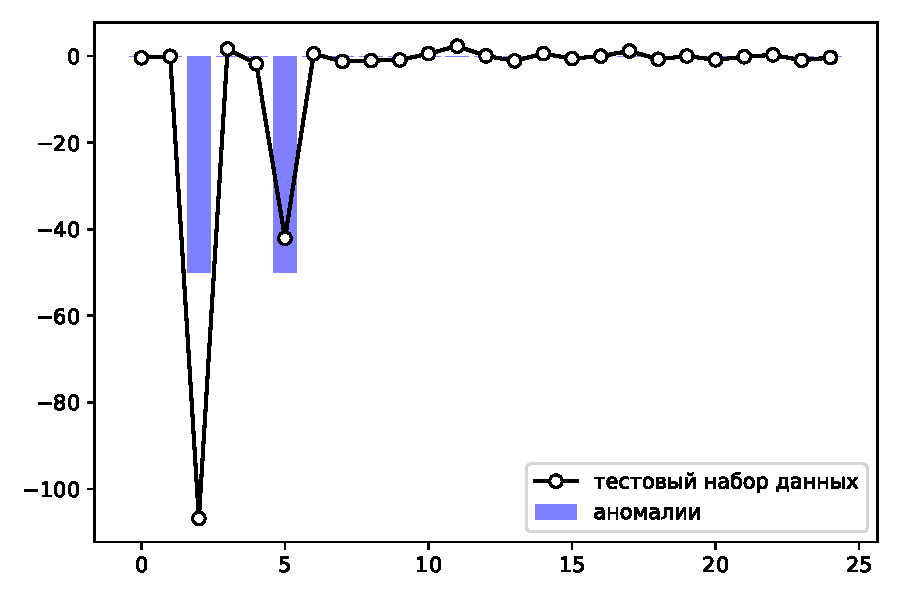
\includegraphics[scale=0.55]{figures/oneclasssvm_test.pdf}
	\caption{ Пример детектирования аномалий на тестовой наборе данных }\label{fig:oneclasssvm}
\end{figure}

Кластеризация. Данная методика предполагает группировку похожих экземпляров в кластеры и не требует знаний о свойствах возможных отклонений: нормальные данные образуют большие плотные кластеры, а аномальные -- маленькие и разрозненные. Одной из простейших реализацией подхода на основе кластеризации является алгоритм метода $ k $-средних.

При использовании методов статистического анализа исследуется процесс, строится его профиль (статистическая модель), которые затем сравнивается с реальным поведением. Если разница в реальном и предполагаемом поведении системы, определяется заданной функцией аномальности, выше установленного порога, делается вывод о наличии отклонений. Применяется предположении о том, что нормальное поведение системы будет находиться в зоне высокой вероятности, в то время как выбросы -- в зоне низкой.

Данный класс методов удобен тем, что не требует заранее определенных знаний о виде аномалии. Однако сложности могут возникать в определении точного статистического распределения и порога.

Методы статистического анализа подразделяются на две группы:
\begin{itemize}
	\item \emph{Параметрические методы}. Предполагают, что нормальные данные генерируются параметрическим распределением с параметрами $ \theta $ и функцией плотности вероятности $ \mathbb{P}(x, \theta) $, где $ x $ -- наблюдение. Аномалия является обратной функцией распределения. Эти методы часто основываются на Гауссовской или регрессионной модели, а также их комбинации.
	
	\item Непараметрические методы. Предполагается, что структура модели не определена априорно, вместо этого она определяется из предоставленных данных. Включает методы на основе гистограмм или функции ядра.
\end{itemize}

Базовый алгоритм поиска аномалий с применением гистограмм включает два этапа. На первом этапе происходит построение гистограммы на основе различных значений выбранной характеристики для экземпляров тренировочных данных. На втором этапе для каждого из исследуемых экземпляров определяется принадлежность к одному из столбцов гистограммы. Не принадлежащие ни к одному из столбцов экземпляры помечаются как аномальные.

Алгоритм ближайшего соседа. Для использования данной методики необходимо определить понятие расстояния (меры похожести) между объектами. Примером может быть евклидово расстояние.

Два основных подхода основаваются на следующих предположениях:
\begin{itemize}
	\item Расстояние до $ k $-ого ближайшего соседа. Для реализации этого подхода расстояние до ближайшего объекта определяется для каждого тестируемого экземпляра класса. Экземпляр, являющийся выбросом, наиболее отдален от ближайшего соседа.
	
	\item Использование относительной плотности основано на оценке плотности окрестности каждого экземпляра данных. Экземпляр, который находится в окрестности с низкой плотностью, оценивается как аномальный, в то время как экземпляр в окрестности с высокой плотностью оценивается как нормальный. Для данного экземпляра данных расстояние до его $ k $-ого ближайшего соседа эквивалентно радиусу гиперсферы с центром в данном экземпляре и содержащей $ k $ остальных экземпляров.
\end{itemize}

Выявление аномалий в режиме реального времени может потребовать дополнительной модификации методов. Наиболее простым в реализации является \emph{алгоритм скользящего окна}.

Данная методика используется для временных рядов, которые разбиваются на некоторое число последовательностей -- окон. Необходимо выбрать окно фиксированной длины, меньшей чем длина самого временного ряда, чтобы захватить аномалию в процессе скольжения. Поиск аномальной последовательности осуществляется при помощи скольжения окна по всему ряду с шагом, меньшим длины окна.


\subsection{Приемы работы с библиотекой \texttt{Prophet}}

Установить библиотеку можно с помощью менеджера пакетов \texttt{conda}
\begin{lstlisting}[
style = bash,
numbers = none
]
conda install -c conda-forge fbprophet
\end{lstlisting}

\texttt{Prophet} была разработана для прогнозирования большого числа различных бизнес-показателей и строит неплохие baseline-прогнозы.

По сути Prophet-модель представляет собой \emph{аддитивную регрессионную модель}
\begin{align*}
	y(t) = g(t) + s(t) + h(t) + \varepsilon_t,
\end{align*}
где $ g(t) $ -- тренд (может быть представлен \emph{кусочно-линейной} или \emph{логистической функцией}\footnote{Логистическая функция удобна для моделирования роста с насыщением, когда при увеличении показателя снижается темп его роста}); $ s(t) $ -- сезонная компонента, отвечающая за периодические/квазипериодические изменения, связанные с \emph{недельной} и \emph{годовой сезонностью}\footnote{Моделируется с помощью рядов Фурье}; $ h(t) $ -- отвечает за аномальные дни (праздники, Black Fridays и т.д.); $ \varepsilon $ -- содержит информацию, которая не учтена моделью.

Подробнее о математической стороне вопроса рассказывается в статье \url{https://peerj.com/preprints/3190/}. К слову, в этой статье качество моделей оценивается с помощью MAPE и MAE. MAPE (mean absolute percentage error) -- это средняя абсолютная ошибка нашего прогноза. Пусть $ y_i $ -- значение целевого вектора, а $ \hat{y}_i $ -- это соответствующий этой величине прогноз модели. Тогда $ \varepsilon_i = y_i - \hat{y}_i $ -- это ошибка прогноза, а $ p_i = \frac{\varepsilon_i}{y_i} $ -- относительная ошибка прогноза.

Таким образом средняя абсолютная ошибка выражается следующей формулой
$$
MAPE = \frac{1}{N}\sum_{i = 1}^{N} |p_i|.
$$

MAPE часто используется для оценки качества, поскольку эта величина относительная и по ней можно сравнивать качество даже на различных наборах данных.

Библиотека \texttt{Prophet} имеет интерфейс, похожий на интерфейс \texttt{sklearn}: сначала мы создаем модель, затем вызываем у нее метод \texttt{fit} и затем получаем прогноз. На вход метод \texttt{fit} получает объект DataFrame с двумя столбцами: \texttt{ds} -- временная метка (поле должно иметь тип \texttt{date} или \texttt{timestamp}), и целевой показатель \texttt{y}.

Разработчики рекомендуют делать предсказания по нескольким месяцам данных (в идеале год и более).

Пример
\begin{lstlisting}[
style = ironpython,
numbers = none
]
import fbprophet
from fbprophet.plot import add_changepoints_to_plot
import pandas as pd
import matplotlib.pyplot as plt


data_all = pd.read_csv('AirPassengers.csv')
# в наборе данных, на котором обучается модель обязательно должны быть столбцы `ds` и `y`
data_all = data_all.rename(columns={ 'Month' : 'ds', 'Passengers' : 'y' })
data_all['ds'] = pd.to_datetime(data_all['ds'])
M = 100
data_train = data_all[:M]  # обучающий набор данных
data_test = data_all[M:]   # тестовый набор данных

model = fbprophet.Prophet(
    changepoint_prior_scale=0.035,
    weekly_seasonality=True,
    yearly_seasonality=True,
    seasonality_mode='multiplicative'
)
model.fit(data_train)  # обучение модели

future_points = data_test.shape[0]  # число точек прогнозного горизонта
# преобразование в точек в метки, имеющие смысл времени
time_points_for_predict = model.make_future_dataframe(future_points, freq='M')
forecast = model.predict(time_points_for_predict)  # прогноз

fig, ax = plt.subplots(figsize=(8, 4))
plt.plot(data_train['ds'], data_train['y'], marker='.', label='Train data')
plt.plot(data_test['ds'], data_test['y'], marker='.', color='k', label='Test data')
plt.plot(forecast['ds'][M:], forecast['yhat'][M:], marker='.', color='r', label='Predict')
plt.axvspan(forecast['ds'][M],forecast['ds'][M+43], facecolor='grey', alpha=0.25)
plt.legend()
# добавить точки перегиба
a = add_changepoints_to_plot(fig.gca(), model, forecast)
\end{lstlisting}

С помощью конструкции \lstinline{model.plot_components(forecast);} можно посмотреть компоненты временного ряда (тренд, недельную и годовую сезонность).

\begin{figure}[h]
	\centering
	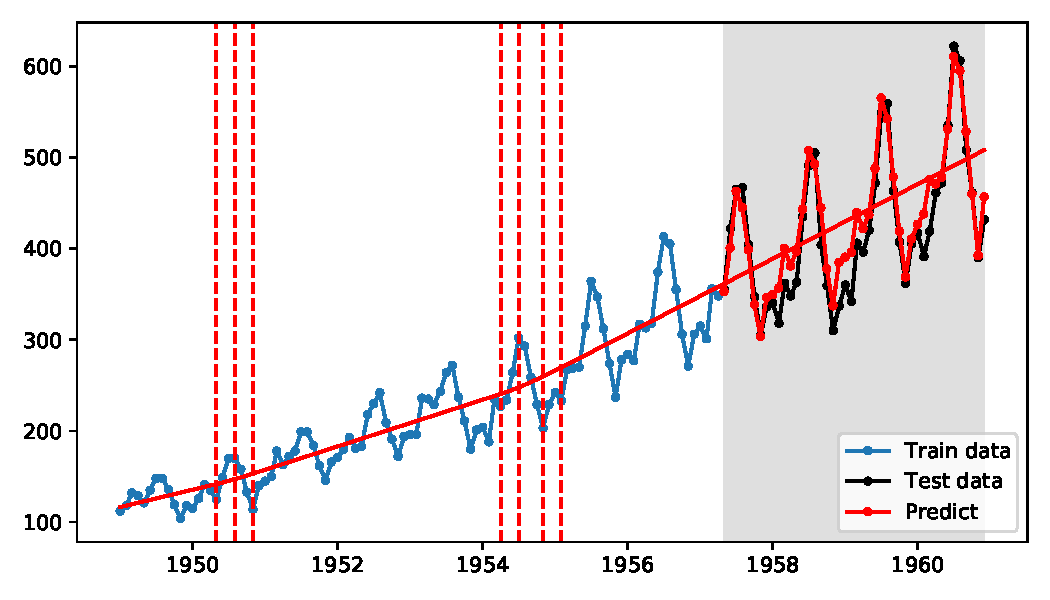
\includegraphics[scale=0.65]{figures/prophet_test.pdf}
	\caption{Пример использования библиотеки \texttt{fbprophet}}\label{fig:prophet_test}
\end{figure}

С помощью библиотеки \texttt{Prophet} можно учитывать эффекты <<праздников>>. Под термином <<праздник>> здесь понимается как <<настоящие>> официальные праздничные и выходные дни (например, Новый Год, Рождество и пр.), так и другие события, во время которых свойства моделируемой зависимой переменной существенно изменяются (спортивные или культурные мероприятия, природные явления и пр.).

Для добавления эффектов <<праздников>> в Prophet-модель необходимо сначала создать отдельную таблицу, содержащую как минимум два обязательных столбца: \texttt{holiday} и \texttt{ds}. Важно, чтобы эта таблица охватывала как исторический период, на основе которого происходит обучение модели, так и период в будущем, для которого необходимо сделать прогноз. Например, если какое-то важное событие встречается в обучающих данных, то его следует указать и для прогнозного периода (при условии, конечно, что мы ожидаем повторение этого события в будущем, и что дата этого события входит в прогнозный период).

Параметры класса \texttt{Prophet}:
\begin{itemize}
	\item \texttt{growth}: тип тренда. Принимает два возможных значения: linear и logistic,
	
	\item \texttt{changepoints}: список временных меток, соответствующих точкам излома тренда (т.е. датам, когда, как предполагается, произошли существенные изменения в тренде временного ряда). Если этот список не задан, то такие точки излома будут вычисляться автоматически,
	
	\item \texttt{n\_changepoints}: предполагаемое количество, точек излома (по умолчанию 25). Если параметр \texttt{changepoints} задан, то параметр \texttt{n\_changepoints} будет проигнорирован. Если же \texttt{changepoints} не задан, то \texttt{n\_changepoints} потенциальных точек излома будут распределены равномерно в предалах исторического отрезка, заданного параметром \texttt{changepoint\_range},
	
	\item \texttt{changepoint\_range}: доля исторических данных (начиная с самого первого наблюдения), в пределах которых будут оценены точки излома. По умолчанию составляет 0.8 (т.е. 80\% наблюдений),
	
	\item \texttt{yearly\_seasonality}: параметр настройки годовой сезонности (т.е. закономерных колебаний в пределах года). Принимает следующие возможные значения: auto, True, False или количество членов ряда Фурье, с помощью которого аппроксимируются компоненты годовой сезонности,
	
	\item \texttt{weekly\_seasonality}: параметр настройки недельной сезонности (т.е. закономерных колебаний в пределах недели). Возможные значения те же, что и у \texttt{yearly\_seasonality},
	
	\item \texttt{daily\_seasonality}: параметр настройки дневной сезонности (т.е. закономерных колебаний в пределах дня). Возможные значения те же, что и у \texttt{yearly\_seasonality},
	
	\item \texttt{holidays}: объект-DataFrame со столбцами \texttt{holiday} и \texttt{ds}. По желанию можно добавить еще два столбца -- \texttt{lower\_window} и \texttt{upper\_window}, которые задают отрезок времени вокруг соответствующего события,
	
	\item \texttt{seasonality\_mode}: режим моделирования сезонных компонент. Принимает два возможных значения: additive и multiplicative,
	
	\item \texttt{seasonality\_prior\_scale}: параметр, задающий <<силу>> сезонных компонентов модели (10 по умолчанию). Более высокие значения приведут к более <<гибкой>> модели, а низкие -- к модели со слабо выраженными сезонными эффектами,
	
	\item \texttt{holidays\_prior\_scale}: параметр, задающий выраженность эффектов <<праздников>> и других важных событий (по умолчанию 10). Если объект-DataFrame, передаваемый в параметр \texttt{holidays}, имеет столбец \texttt{prior\_scale}, то параметр \texttt{holidays\_prior\_scale} будет проигнорирован,
	
	\item \texttt{changepoint\_prior\_scale}: параметр, задающий <<гибкость>> автоматического механизма обнаружения <<точек излома>> (по умолчанию 0.05). Более высокие значения позволят иметь больше таких точек излома,
	
	\item \texttt{mcmc\_samples}: целое число (по умолчанию 0). Если $ > 0 $, то параметры модели будут оценены путем \emph{полного байесовского анализа} с использованием указанного числа итераций алгоритма MCMC. Если 0, тогда используется \emph{оценка апостериорного максимума} (MAP),
	
	\item \texttt{interval\_width}: число, определяющее ширину доверительного интервала для предсказанных моделью значений (по умолчанию 0.8, что соответствует 80\%-ному интервалу),
	
	\item \texttt{uncertainty\_samples}: количество итераций для оценивания доверительных интервалов (по умолчанию 1000).
\end{itemize}

\emph{Оценка максимума апостериорной вероятности} (maximum aposteriori probability, MAP) тесно связана с \emph{методом наибольшего правдоподобия} (ML), но дополнительно при оптимизации использует априорное распределение величины, которую оценивает.

Можно записать
\begin{align*}
	\hat{\theta}_{\rm MAP}(x) = \underset{\theta}{\operatorname{arg\,max}}\, f(x | \theta)g(\theta),
\end{align*}
где $ f(x | \theta) $ -- функция правдоподобия, $ g(\theta) $ -- априорная плотность распределения оцениваемого параметра $ \theta $.

Пример. Предположим, что у нас есть последовательность $ (x_1, \dots, x_n) $ i.i.d (независимых и одинаково распределенных) $ N(\mu, \sigma_v^2) $ случайных величин и априорное распределение $ \mu $ задано $ N(0, \sigma_m^2) $. Требуется найти MAP-оценку $ \mu $.

Функция, которую нужно максимизировать задана
\begin{align*}
	\pi(\mu)L(\mu) = \dfrac{1}{\sqrt{2\pi \sigma_m}} \exp \Bigg( - \dfrac{1}{2}\Big(\dfrac{\mu}{\sigma_m}\Big)^2 \Bigg) \prod_{j=1}^{n} \dfrac{1}{\sqrt{2\pi \sigma_v}} \exp \Bigg( -\dfrac{1}{2}\Big( \dfrac{x_j - \mu}{\sigma_v} \Big)^2 \Bigg).
\end{align*}

Теперь остается записать логарифм этой функции, затем найти производную по оцениваемому параметру, приравнять полученную производную нулю и, наконец, выразить искомый параметр. Что в итоге даст
\begin{align*}
    \hat{\mu}_{\rm MAP} = \dfrac{\sigma_m^2}{n\sigma_m^2 + \sigma_v^2} \sum_{j=1}^{n}x_j.
\end{align*}

\subsubsection{Настройка гиперпараметров}

Настройка гиперпараметров выполняется следующим образом
\begin{lstlisting}[
style = ironpython,
numbers = none	
]
import itertools
import numpy as np
import pandas as pd

param_grid = {
	'changepoint_prior_scale': [0.001, 0.01, 0.1, 0.5],
	'seasonality_prior_scale': [0.01, 0.1, 1.0, 10.0],
}

# Generate all combinations of parameters
all_params = [
    dict(zip(param_grid.keys(), v))
    for v in itertools.product(*param_grid.values())
]
rmses = []  # Store the RMSEs for each params here

# Use cross validation to evaluate all parameters
for params in all_params:
    m = Prophet(**params).fit(df)  # Fit model with given params
    df_cv = cross_validation(
        m,
        cutoffs=cutoffs,
        horizon='30 days',
        parallel="processes"
     )
    df_p = performance_metrics(df_cv, rolling_window=1)
    rmses.append(df_p['rmse'].values[0])

# Find the best parameters
tuning_results = pd.DataFrame(all_params)
tuning_results['rmse'] = rmses
print(tuning_results)
\end{lstlisting}

Перечень параметров, которые имеет смысл настраивать:
\begin{itemize}
	\item \texttt{changepoint\_prior\_scale}: это, вероятно, самый важный параметр. Он определяет \emph{гибкость тренда}. И в частности насколько сильно меняется тренд в точках изменения тренда. Значение по умолчанию (0.05), как правило, работает корректно. Более высокие значения позволят иметь больше точек излома тренда. Если основания считать, что настройка этого параметра улучшит модель, то имеет смысл рассмотреть диапазон $ [0.001; 0.5] $.
	
	\item \texttt{seasonality\_prior\_scale}: этот параметр определяет гибкость сезонности. Значение по умолчанию (10) работает для большинства случаев, но если есть основания считать, что настройка этого параметра улучшит модель, то имеет смысл рассмотреть диапазон $ [0.01; 10] $.
	
	\item \texttt{holidays\_prior\_scale}: управляет гибкостью настройки эффекта праздников.
	
	\item \texttt{seasonality\_mode}: лучше настраивать, просто посмотрев на временной ряд.
\end{itemize}

Перечень параметров, которые можно было бы попробывать настроить:
\begin{itemize}
	\item \texttt{changepoint\_range}
\end{itemize}

Перечень параметров, которые нет смысла настраивать:
\begin{itemize}
	\item \texttt{growth},
	
	\item \texttt{changepoints},
	
	\item \texttt{n\_changepoints},
	
	\item \texttt{yearly\_seasonality},
	
	\item \texttt{weekly\_seasonality},
	
	\item \texttt{daily\_seasonality},
	
	\item \texttt{holidays},
	
	\item \texttt{mcmc\_samples},
	
	\item \texttt{interval\_width},
	
	\item \texttt{uncertainty\_samples},
	
	\item \texttt{stan\_backend}.
\end{itemize}


\subsection{Преобразование нестационарного временного ряда в стационарный}

Чтобы превратить нестационарный ряд в стационарный можно использовать следующие общие приемы:
\begin{itemize}
	\item выделить в структуре временного ряда тренд и сезонную компоненту, затем удалить их исходного временного ряда; построить прогноз на временном ряду, приведенном к стационарному, а после вернуть эти компоненты в прогноз,
	
	\item провести сглаживание (за несколько часов, за неделю и т.п.); в простейших случаях, когда период временного четко определен, можно пользоваться обычным скользящим средним, но в более сложных случаях, когда период сложно подсчитать, следует пользоваться \emph{экспоненциально-взвешенным скользящим средним}
	\lstinline{time_series.ewm(halflife=12).mean()}.
\end{itemize}


\subsection{Стабилизация дисперсии}

Для временных рядов с \emph{монотонно} меняющейся дисперсией можно использовать стабилизирующие преобразования. Например, \emph{логарифмирование} \lstinline{np.log(ts)}.

Если исходный временной ряд не проходит тест на \emph{гауссовость}, то можно либо воспользоваться непараметрическими методами, либо обратиться к специальным приемам, позволяющим преобразовать исходную ненормальную статистику в нормальную.

Среди множества таких методов преобразований одним из лучших (при неизвестном типе распределения) считается \href{http://www.machinelearning.ru/wiki/index.php?title=Метод_Бокса-Кокса}{\itshape преобразование Бокса-Кокса}\footnote{Степенные преобразования -- это семейство параметрических, монотонных преобразований, целью которых является отображение данных из произвольного распределения в близкое к гауссовскому распределению таким образом, чтобы \emph{стабилизировать дисперсию} и \emph{минимизировать ассиметрию}}, то есть это преобразование \emph{нормализует} данные (делает их более гауссовскими)
\begin{align*}
	\hat{y}_i =
	\begin{cases}
		\log y_i, &\lambda = 0,\\
		(y_i^\lambda - 1)/\lambda, &\lambda \neq 0
	\end{cases}
\end{align*}
для исходной последовательности $ y = \{y_1, \dots, y_n\}, \,y_i > 0,\, i = (1, \dots, n) $.

Пример использования преобразования Бокса-Кокса приведен на \pic{fig:boxcox}. Такого рода преобразования полезны в ситуациях, связанных с проблемой \emph{гетероскедостичности} (непостоянная дисперсия), или в ситуациях, где требуется \emph{гауссовость} данных.

\begin{figure}[h]
	\centering
	\includegraphics[scale=0.70]{figures/boxcox.pdf}
	\caption{Влияние преобразования Бокса-Кокса на временной ряд\\с изменяющейся во времени дисперсией}\label{fig:boxcox}
\end{figure}

Параметр $ \lambda $ можно подбирать так, чтобы дисперсия была как можно более стабильной во времени. Прямое и обратное преобразования Бокса-Кокса реализованы в библиотеках \texttt{scipy} и \texttt{statsmodels}
\begin{lstlisting}[
style = ironpython,
emph = {invboxcox},
numbers = none
]
from scipy.stats import boxcox
from statsmodels.tsa.hotwinters import (
                                        #boxcox,
                                        inv_boxcox
                                        )

# пользуемся готовым решением для обратного преобразования Бокса-Кокса
lmbda = 0.25
arr = np.array([3, 5, 10])
# можно задать значение ламбда самому или позволить вычислить его
arr_transformed = boxcox(arr, lmbda) # array([1.26429605, 1.98139512, 3.11311764])
arr_transformed, lmbda_compute = boxcox(arr)  # здесь lmbda вычисляется
                                              # с помощью максимизации логарифма правдоподобия
inv_boxcox(arr_transformed, lmbda)  # array([ 3.,  5., 10.])

# пишем свою реализацию обратного преобразования Бокса-Кокса
def invboxcox(arr: np.array, lmbda: np.float) -> np.array:
    if lmbda == 0:
        return (np.exp(arr))
    else:
        return (np.exp(np.log(lmbda*arr + 1)/lmbda))
\end{lstlisting}

Так как классическое преобразование Бокса-Кокса предполагает работу только с положительными величинами, то было предложено несколько модификаций, учитывающих нулевые и отрицательные значения. Самым очевидным вариантом является сдвиг всех значений на некоторую константу $ \alpha $ так, чтобы выполнялось условие $ (y_i + \alpha) > 0, \, i = 1,\dots, n $
\begin{align*}
	\hat{y}_i =
	\begin{cases}
		\log (y_i + \alpha), &\lambda = 0,\\
		\dfrac{(y_i + \alpha)^\lambda - 1}{\lambda}, &\lambda \neq 0.
	\end{cases}
\end{align*}

Также для того чтобы сделать данные <<более гауссовскими>> можно воспользоваться \emph{преобразованием Йео-Джонсона} (Yeo-Johnson)
\begin{align*}
	\hat{y}_i = 
	\begin{cases}
		\dfrac{(y_i + 1)^\lambda - 1}{\lambda}, &\lambda \neq 0, y_i \geqslant 0,\\
		\ln(y_i + 1), &\lambda = 0, y_i \geqslant 0,\\
		- \dfrac{(-y_i + 1)^{2 - \lambda} - 1}{2 - \lambda}, &\lambda \neq 2, y_i < 0,\\
		-\ln(-y_i + 1), &\lambda = 2, y_i < 0.
	\end{cases}
\end{align*}

Преобразование Йео-Джонсона (как впрочем и преобразование Бокса-Кокса) реализовано в библиотеке \texttt{sklearn} (см.~раздел документации \href{https://scikit-learn.org/stable/modules/preprocessing.html#preprocessing-transformer}{Non-linear transformation})
\begin{lstlisting}[
style = ironpython,
numbers = none
]
import numpy as np
from sklearn.preprocessing import PowerTransformer
yj = PowerTransformer(method='yeo-johnson')
bc = PowerTransformer(method='box-cox', standardize=False)

data_log = np.random.RandomState(616).lognormal(size=(3,3))
yj.fit_transform(data_log)  # вернет новое представление данных
\end{lstlisting}

\remark{%
Преобразование Бокса-Кокса требует, чтобы значения набора данных были строго положительными, в то время как преобразование Йео-Джонсона может работать как с положительными, так и с отрицательными значениями
}


\section{Методологии проектирования реляционного хранилища данных}

\subsection{Основная терминология}

Data Vault -- гибридный подход, объединивший достоинства схемы <<звезда>> и третьей нормальной формы. Состоит из трех основных компонентов (\pic{fig:base_scheme_data_vault}) -- хабов (Hub), ссылок (Link) и сателлитов (Satellite).

\begin{figure}[h]
	\centering
	\includegraphics[scale=0.65]{figures/base_scheme_data_vault.png}
	\caption{ Пример хранилища, построенного с помощью подхода Data Vault }\label{fig:base_scheme_data_vault}
\end{figure}


\emph{Хаб} -- основное представление сущности (Клиент, Продукт, Заказ) с позиций бизнеса. Таблица-хаб содержит одно или несколько полей, отражающих сущность в понятиях бизнеса. В совокупности эти поля называются <<бизнес-ключ>>. Идеальный кандидат на звание бизнес-ключа это ИНН организации или VIN номер автомобиля, а сгенерированный системой ID будет наихудшим вариантом. Бизнес-ключ всегда должен быть уникальным и неизменяемым. Хаб также содержит мета-поля load timestamp и record source, в которых храняться время первоначальной загрузки сущности в хранилище и ее источник (название системы, базы или файла, откуда данные были загружены). В качестве первичного ключа Хаба рекомендуется использовать MD5 или SHA-1 хеш от бизнес-ключа.

\emph{Ссылка} -- связь типа <<многие-ко-многим>>, связывающая несколько хабов. Она содержит те же метаданные, что и хаб. Ссылка может быть связана с другой ссылкой, но такой подход создает проблемы при загрузке, так что лучше выделить одну из ссылок в отдельный хаб.

Все описательные атрибуты Хаба или Ссылки (контекст) помещаются в \emph{таблицы-Сателлиты}. Помимо контекста Сателлит содержит стандартный набор метаданных (load timestamp и record source) и \emph{один и только один ключ <<родителя>>}. В Сателлитах можно без проблем хранить историю изменения контекста, каждый раз добавляя новую запись при обновлении контекста в системе-источнике. Для упрощения процесса обновления большого сателлита в таблицу можно добавить поле hash diff: MD5 или SHA-1 хеш от всех его описательных атрибутов. Для Хаба или Ссылки может быть сколь угодно Сателлитов, обычно контекст разбивается по частоте обновления. Контекст из разных систем-источников принято класть в отдельные Сателлиты.

Сначала данные из операционных систем поступают в staging area. Staging area используется как промежуточное звено в процессе загрузки данных. Одна из основных функций Staging зоны это снижение нагрузки на операционные базы при выполнении запросов. Таблицы здесь полностью повторяют исходную структуру, но любые ограничения на вставку данных, вроде not null или проверки целостности внешних ключей, должны быть выключены с целью оставить возможность вставить даже поврежденные или неполные данные (особенно это актуально для excel-таблиц и прочих файлов). Дополнительно в stage таблицах содержатся хеши бизнес-ключей и информация о времени загрузки и источнике данных (\pic{fig:dwh_data_vault}).

\begin{figure}[h]
	\centering
	\includegraphics[scale=0.65]{figures/dwh_data_vault.png}
	\caption{ Высокоуровненвое представление хранилища данных }\label{fig:dwh_data_vault}
\end{figure}

После этого данные разбиваются на Хабы, Ссылки и Сателлиты и загружаются в Raw Data Vault (в процессе загрузки они никак не агрегируются и не пересчитываются).

Business Vault — опциональная вспомогательная надстройка над Raw Data Vault. Строится по тем же принципам, но содержит переработанные данные: агрегированные результаты, сконвертированные валюты и прочее. Разделение чисто логическое, физически Business Vault находится в одной базе с Raw Data Vault и предназначен в основном для упрощения формирования витрин.

Когда нужные таблицы созданы и заполнены, наступает очередь витрин данных (Data Marts). Каждая витрина это отдельная база данных или схема, предназначенная для решения задач различных пользователей или отделов. В ней может быть специально собранная «звезда» или коллекция денормализованных таблиц. Если возможно, \emph{таблицы} внутри \emph{витрин} лучше делать \emph{виртуальными}, то есть вычисляемыми <<на лету>>. Для этого обычно используются SQL представления (SQL views).

Заполняется Data Vault следующим образом: сначала загружаются Хабы, потом Ссылки и затем Сателлиты; Хабы можно загружать параллельно, так же как и Сателлиты и Ссылки, если конечно не используется связь link-to-link.

Преимущества и недостатки
\begin{itemize}
	\item (+) Гибкость и расширяемость. С Data Vault перестает быть проблемой как расширение структуры хранилища, так и добавление и сопоставление данных из новых источников. Максимально полное хранилище «сырых» данных и удобная структура их хранения позволяют нам сформировать витрину под любые требования бизнеса, а существующие решения на рынке СУБД хорошо справляются с огромными объемами информации и быстро выполняют даже очень сложные запросы, что дает возможность виртуализировать большинство витрин,
	
	\item (+) Agile-подход из коробки. Моделировать хранилище по методологии Data Vault довольно просто. Новые данные просто <<подключаются>> к существующей модели, не ломая и не модифицируя существующую структуру. При этом поставленная задача решается максимально изолировано,
	
	\item (-) Обилие соединений. За счет большого количества операций соединения запросы могут быть медленее, чем в традиционных хранилищах данных, где таблицы денормализованы,
	
	\item (-) Сложность. В описаной выше методологии есть множество важных деталей, разобраться в которых вряд ли получится за пару часов. К этому можно прибавить малое количество информации. Как следствие, при внедрении Data Vault возникают проблемы с обучением команды. Большой недостаток -- это обязательное требование наличия витрин данных, так как сам по себе Data Vault плохо подходят для прямых запросов,
	
	\item (-) Избыточность.
\end{itemize}


\subsection{Базовые сведения о концепциях}

Многое в жизни проекта зависит от того, насколько хорошо продумана объектная модель и структура базы на старте.

Общепринятым подходом были и остаются различные варианты сочетания схемы <<звезда>> с третьей нормальной формой. Как правило, по принципу: исходные данные — 3NF, витрины — звезда. Этот подход, проверенный временем и подкрепленный большим количеством исследований — первое (а иногда и единственное), что приходит в голову опытному DWH-шнику при мысли о том, как должно выглядеть \emph{аналитическое} хранилище.

С другой стороны данные могут расти как <<вглубь>>, так и  <<вширь>>. И вот тут проявляется основной недостаток звезды -- \emph{ограниченная гибкость}.

Ниже рассматриваются две самые популярные для хранилищ данных методологии гибкого проектирования -- Anchor model и Data Vault. За скобками остаются такие приемы, как, например, \href{https://en.wikipedia.org/wiki/Entity–attribute–value_model}{EAV}\footnote{Это модель данных для кодирования пространственно-эффективным способом сущностей, в которых число атрибутов (свойств, параметров) потенциально огромно, но число фактически применяемых к данной сущности относительно мало. Такие сущности соответствуют математическому понятию разреженной матрицы} (Entity-attribute-value), 6NF и все относящееся к NoSQL решениям.

\paragraph{Проблемы <<классического>> подхода и их решения в гибких методологиях} Во-первых, в основу такой модели закладывается четкое разделение данных на \emph{измерения} и \emph{факты}. И это логично. Ведь в подавляющем большинстве случаев анализ сводится именно к анализу определенных числовых показателей (фактов) в определенных разрезах (измерениях).

При этом связи между объектами закладываются в виде связей между таблицами по внешнему ключу. Это выглядит вполне логично, но сразу же приводит к первому ограничению гибкости -- жесткому определению кардинальности связей.

Это значит, что на этапе прокетирования таблиц нужно точно определить для каждой пары связанных объектов могут ли они относиться как многие-ко-многим, или только как 1-ко-многим, и <<в какую сторону>>. От этого напрямую зависит в какой из таблиц будет первичный ключ, а в какой -- внешний. Изменение этого отношения при получении новых требований с большой вероятностью приведет к переработке базы данных.

В Data Vault таблицы-связки называют Link, а в Якорной модели -- Tie. В обеих архитектурах таблицы-связки могут связывать любое количество сущностей.

Эта на первый взгляд избыточность дает существенную гибкость при доработках (\pic{fig:links}).

\begin{figure}[h]
	\centering
	\includegraphics[scale=0.85]{figures/links.png}
	\caption{ Пример Структура толерантная к изменению кардинальности существующих связей }\label{fig:links}
\end{figure}

\paragraph{Хранение объектов и атрибутов в Data Vault и Anchor Model} Подход, предлагаемый авторами гибких архитектур, можно сформулировать так: необходимо отделить то, что изменяется, от того, что остается неизменным; то есть хранить ключи отдельно от атрибутов.

Точки зрения на то, что именно можно считать неизменным в Data Vault и Якорной модели расходятся. С точки зрения архитектуры Data Vault, неизменным можно считать весь набор ключей -- натуральные (ИНН организации, код товара в системе-источнике и т.п.) и суррогатные\footnote{Сурогатный ключ -- это искусственно введенный в отношение атрибут, предназначенный исключительно для идентификации кортежей в отношении. Другими словами, суррогатный ключ не образовывается на основании каких-либо существующих атрибутах отношения, а генерируется искусственно}. При этом остальные атрибуты можно разделить на группы по источнику и/или частоте изменений и для каждой группы вести отдельную таблицу с независимым набором версий.

В Anchor Model неизменным считается только суррогатный ключ сущности. Все остальное (включая натуральные ключи) -- просто частный случай его атрибутов. При этом все атрибуты по умолчанию независимы друг от друга, поэтому для каждого атрибута должна быть создана отдельная таблица.

В Data Vault таблицы, содержащие ключи сущностей, называются Хабами (Hub). Хабы всегда содержат фиксированный набор полей:
\begin{itemize}
	\item Натуральные ключи сущности,
	
	\item Суррогатный ключ,
	
	\item Ссылку на источник,
	
	\item Время добавления записи.
\end{itemize}

Записи в Хабах никогда не изменяются и не имеют версий. Внешне хабы очень похожи на таблицы типа ID-map, применяемые в некоторых системах для генерации суррогатов, однако в качестве суррогатов в Data Vault рекомендуется применять не целочисленный сиквенс, а хэш от набора бизнес-ключей. Такой подход упрощает загрузку связей и атрибутов из источников, но может вызвать другие проблемы (поэтому не является общепринятым).

Все остальные атрибуты сущностей хранятся в специальных таблицах, называемых Сателлитами. Один хаб может иметь несколько сателлитов, хранящих разные наборы атрибутов.

Распределение атрибутов по сателлитам происходит по принципу совместного изменения -- в одном сателлите могут храниться не версионные атрибуты (например, дата рождения и СНИЛС для физ. лица), в другом -- редко изменяющиеся версионные (например, фамилия и номер паспорта), в третьем -- часто изменяющиеся (например, адрес доставки, категория, дата последнего заказа и т.п.).

Версионность при этом ведется на уровне отдельных сателлитов, а не сущности в целом, поэтому распределение атрибутов целесообразно проводить так, чтобы пересечение версий внутри одного сателлита было минимальным (что сокращает общее количество хранимых версий).

Также, для оптимизации процесса загрузки данных, в отдельные сателлиты часто выносятся атрибуты, получаемые из различных источников. Сателлиты связываются с хабом по внешнему ключу (что соответствует связи один-ко-многим). Это значит, что множественные значения атрибутов (например, несколько контактных номеров телефона у одного клиента) поддерживается такой архитектурой по умолчанию.

В Якорной модели таблицы, хранящие ключи, называются Якорями (Anchor) и хранят они:
\begin{itemize}
	\item только суррогатные ключи,
	
	\item ссылку на источник,
	
	\item время добавления записи.
\end{itemize}

Натуральные ключи с точки зрения Якорной модели считаются обычными атрибутами. Например, если данные об одной и той же сущности могут поступать из разных систем, в каждой из которых используется свой натуральный ключ. 

В Data Vault типичный объект для хранения фактов - Связь (Link), в Сателлиты которой складываются вещественные показатели.

Такой подход выглядит интуитивно понятным. Он дает простой доступ к анализируемым показателям и в целом похож на традиционную таблицу фактов (только показатели хранятся не в самой таблице, а в <<соседней>>). Но есть и подводные камни: одна из типовых доработок модели — расширение ключа факта — вызывает необходимость добавления в Link нового внешнего ключа. А это в свою очередь <<ломает>> модульность и потенциально вызывает необходимость доработок других объектов.

В Якорной модели Связь не может иметь собственных атрибутов, поэтому такой подход не прокатит — абсолютно все атрибуты и показатели обязаны иметь привязку к одному конкретному якорю. Вывод из этого простой — для каждого факта тоже нужен свой якорь. Для части того, что мы привыкли воспринимать как факты, это может выглядеть естественно — например, факт покупки прекрасно сводится к объекту <<заказ>> или <<чек>>, посещение сайта — к сессии и т.п. Но встречаются и факты, для которых найти такой естественный <<объект-носитель>> не так просто — например, остатки товаров на складах на начало каждого дня.

Соответственно, проблем с модульностью при расширении ключа факта в Якорной модели не возникает (достаточно просто добавить новую Связь к соответствующему Якорю), но проектирование модели для отображения фактов менее однозначно, могут появляться <<искусственные>> Якоря, отображающие объектную модель бизнеса не очевидно.

Получившаяся конструкция в обоих случаях содержит существенно больше таблиц, чем традиционное измерение. Но может занимать существенно меньше дискового пространства при том же наборе версионных атрибутов, что и традиционное измерение. Никакой магии тут, естественно, нет — всё дело в нормализации. Распределяя атрибуты по Сателлитам (в Data Vault) или отдельным таблицам (Anchor Model), мы уменьшаем (или совсем исключаем) дублирование значений одних атрибутов при изменении других.

Для Data Vault выигрыш будет зависеть от распределения атрибутов по Сателлитам, а для Якорной модели — практически прямо пропорционален среднему количеству версий на объект измерения.

Однако выигрыш по занимаемому месту — важное, но не главное преимущество отдельного хранения атрибутов. Вместе с отдельным хранением связей, такой подход делает хранилище модульной конструкцией. Это значит, что добавление как отдельных атрибутов, так и целых новых предметных областей в такой модели выглядит как надстройка над существующим набором объектов без их изменения. И это именно то, что делает описанные методологии гибкими.

Декомпозиция данных, лежащая в основе модульности гибких архитектур, приводит к увеличению количества таблиц и, соответственно, накладных расходов на джойны при выборке. Для того, чтобы просто получить все атрибуты измерения, в классическом хранилище достаточного одного селекта, а гибкая архитектура потребует целого ряда джойнов. Причем если для отчетов все эти джойны можно написать заранее, то аналитики, привыкшие писать SQL руками, будут страдать вдвойне.

Многое зависит от движка. У многих современных платформ есть внутренние механизмы оптимизации джойнов. Например, MS SQL и Oracle умеют <<пропускать>> джойны на таблицы, если их данные не используются нигде, кроме других джойнов и не влияют на финальную выборку (table/join elimination), а \emph{MPP Vertica} по опыту коллег из Авито, показала себя как прекрасный \emph{движок} для \emph{Якорной модели} с учетом некоторой ручной оптимизации плана запроса.

С другой стороны, хранить Якорную модель, например, на Click House, имеющем ограниченную поддержку join, пока выглядит не очень хорошей идеей.

Выводы:
\begin{itemize}
	\item После некоторой начальной подготовки, связанной с развертыванием метаданных и написанием базовых алгоритмов ETL, быстро предоставить заказчику первый результат в виде парочки отчетов, содержащих данные всего нескольких объектов источников. Полностью продумывать (даже верхнеуровнево) всю объектную модель для этого не обязательно,
	
	\item Модель данных может начать работать (и приносить пользу) всего с 2-3 объектами, разрастаясь со временем,
	
	\item Большинство доработок, включая расширение предметной области и добавление новых источников не затрагивает существующий функционал и не вызывает опасность сломать что-то уже работающее,
	
	\item Благодаря декомпозиции на стандартные элементы, ETL-процессы в таких системах выглядят однотипно, их написание поддается алгоритмизации и, в конечном счете, автоматизации.
\end{itemize}

Ценой такой гибкости является производительность. Это не значит, что достигнуть приемлемой производительности на таких моделях невозможно. Чаще всего, просто может потребоваться больше усилий и внимания к деталям для достижения нужных метрик.

Сводная таблица с общими чертами и различиями рассмотренных подходов приведена на \pic{fig:vault_anchor}.

\begin{figure}[h]
	\centering
	\includegraphics[scale=0.65]{figures/vault_anchor.png}
	\caption{ Сводка по гибким методологиям }\label{fig:vault_anchor}
\end{figure}



\section{Кодирование признаков}

Полезная статья про кодировщики и различные стратегии валидации \url{https://towardsdatascience.com/benchmarking-categorical-encoders-9c322bd77ee8}.

Можно использовать готовые алгоритмы кодирования, реализованные в библиотеке\\ \texttt{category\_encoders} \url{https://pypi.org/project/category-encoders/}\footnote{Установить можно как обычно: \texttt{pip install category-encoders}}

Категориальные признаки можно разделить на \emph{порядковые признаки} (например, <<медлено>>, <<быстро>>, <<быстрее>> и т.д.) и \emph{номинальные признаки} (<<кошки>>, <<собаки>> и т.д.).

Основные приемы кодирования категориальных признаков:
\begin{itemize}
	\item для порядковых признаков
	\begin{itemize}
		\item \emph{пользовательское отображение}, которое учитывает определенный порядок (соотношение) категорий, например, \verb|{"cold" : 0, "warm" : 1, "hot" : 2}|: класс \texttt{LabelEncoder} следует применять только (!) для \emph{целевого вектора}, для которого порядок меток не имеет никакого значения; если выполнить кодировку порядкового признака с помощью \texttt{LabelEncoder}, то алгоритм будет предполагать, что между категориями существует порядковая зависимость, то есть их можно как-то отсортировать, а это неверно! \cite[151]{raschka:2019}
	\end{itemize}

    \item для именных признаков
    \begin{itemize}
    	\item \emph{частотное кодирование}: например, с помощью \texttt{category\_encoder.CountEncoder} (затем, разумеется, нужно число элементов в категории разделить на число строк в наборе данных); можно реализовать свой собственный кодировщик 
\begin{lstlisting}[
style = ironpython,
numbers = none
]
train_nominal_freq_enc = train_nominal.copy()
fq = train_nominal.groupby("col_nominal_name").size()/train_nominal.shape[0]
train_nominal_freq_enc["col_nominal_name"] =
    train_nominal_freq_enc["col_nominal_name"].map(fq)
\end{lstlisting}

    \item \emph{кодирование с одним активным состоянием} (еще говорят унитарное кодирование): легко реализовать с помощью \\ \texttt{sklearn.preprocessing.OneHotEncoder} или \\ с помощью \texttt{pd.get\_dummies(df, drop\_first=True)} (параметр \texttt{drop\_first=True} нужен для того, чтобы сократить взаимосвязь между признаками, полученными с помощью техники кодирования с одним активным состоянием, так как унитарное кодирование привносит мультиколлиниарность, что может приводить к появлению неустойчивых оценок \cite[153]{raschka:2019}),
    
    \item \emph{M-вероятностная оценка правдоподобия} (другие варианты: аддитивное сглаживание; кодирование сглаженным средним): можно использовать \\ класс \texttt{category\_encoders.m\_estimate.MEstimateEncoder}. Каждая категория категориального признака кодируются по следующей формуле
    \begin{align*}
        e_k = \dfrac{ s_k^t + m\, \dfrac{s^t}{n} }{c_k + m},\ (k = 1,\ldots, K),
    \end{align*}
    где $ s_k^t $ -- сумма значений целевого вектора для $ k $-ой категории; $ m $ -- степень регуляризации; $ n $ -- длина целевого вектора (число строк в наборе данных); $ c_k $ -- размер $ k $-ой категории (число экземпляров $ k $-ой категории); $ K $ -- число категорий (уникальных значений) категориального признака.
\begin{lstlisting}[
style = ironpython,
numbers = none	
]
from category_encoders.m_estimate import MEstimateEncoder

# здесь m -- это степень регуляризации
me_enc = MEstimateEncoder(m=50)  # рекомендуемые значения для m = [1, 100]

data_mEst_enc = data.copy()
data_mEst_enc["col3"] = me_enc.fit_transform(
    data_mEst_enc.loc[:, "col3"],
    data_mEst_enc.loc[:, "target"]
)
\end{lstlisting}

    \item \emph{взвешенное суждение} (Weight of Evidence \url{https://contrib.scikit-learn.org/category_encoders/woe.html}): чаще всего применяется в кридитном скоринге.
    
    \item \emph{CatBoost-кодировщик}: можно использовать готовый класс \texttt{CatBoostEncoder} \url{https://contrib.scikit-learn.org/category_encoders/catboost.html}\\ из библиотеки \texttt{category\_encoders}; этот кодировщик предназначен для преодоления проблем утечки данных, присущих кодировщику \texttt{Leave-one-out Encoder} (LOO); чтобы предотвратить переобучение, процесс кодирования повторяется несколько раз для перетасованных версий набора данных, а результаты усредняются.
    \end{itemize}
\end{itemize}

Удобно использовать трансформеры столбцов
\begin{lstlisting}[
style = ironpython,
numbers = none	
]
from sklearn.compose import make_column_transformer
from sklearn.preprocessing import OneHotEncoder
from sklearn.pipeline import make_pipeline
from category_encoders.cat_boost import CatBoostEncoder

col_trans = make_column_transformer(
    (OneHotEncoder(sparse=False), ["col2", "col10"]),
    (CatBoostEncoder(), ["col20"])
)

gbm = GradientBoostingRegressor()
gbm_pipeline = make_pipeline(col_trans, gbm)

gbm_pipeline.fit(X_train, y_train)
gbm_pred = gbm_pipeline.predict(X_test)
\end{lstlisting}

Что касается стратегий валидации, то можно выделить 3 основные:
\begin{itemize}
	\item None Validation: очень грубо,
	
	\item Single Validation: что-то среднее между None Validation и Double Validation,
	
	\item Double Validation: очень медленно.
\end{itemize}

\vspace*{2mm}
Стратегия для одиночной валидации:
\begin{enumerate}
	\item Разбиваем имеющийся набор данных на обучение и тест,
	
	\item Обучающий набор данных разбиваем на несколько фолдов,
	
	\item Каждый фолд кодируем своим кодировщиком (т.е. кодировщиков будет столько, сколько было фолдов),
	
	\item На каждом закодированном фолде обучаем свою модель (моделей столько, сколько было фолдов),
	
	\item Кодируем тестовый набор данных теми же кодировщиками, которые мы использовали на этапе обучения (т.е. несколько представлений тестового набора данных),
	
	\item на каждом закодированном тестовом представлении делаем прогноз с помощью моделей, обученных на соответствующих закодированных данных обучающего набора,
	
	\item для получения финального прогноза усредняем прогнозы моделей.
\end{enumerate}




\section{Машинное обучение с AutoML}

На данный момент AutoML представленная следующими направлениями:
\begin{itemize}
	\item AutoML для автоматизации подбора гиперпараметров модели,
	
	\item AutoML для неглубокого обучения,
	
	\item AutoML для глубокого обучения.
\end{itemize}

Список наиболее полезных библиотек:
\begin{itemize}
	\item \texttt{featuretools} \url{https://featuretools.alteryx.com/en/stable/},
	
	\item \texttt{MLBox} \url{https://mlbox.readthedocs.io/en/latest/index.html},
	
	\item \texttt{TransmogrifAI} (Scala API) \url{https://github.com/salesforce/TransmogrifAI}.
\end{itemize}



\section{Хранилища данных. DWH}

Хранилище данных (Data WareHouse, DWH) -- предметно-ориентированная информационная база данных, специально разработанная и предназначенная для подготовки отчетов и безнес-анализа с целью поддержки принятия решений в организации. Строится на основе систем управления базами данных и систем поддержки принятия решений. Данные, поступающие в хранилище данных, как правило, доступны только для чтения.

\remark{%
DWH необходимо для проведения эффективного бизнес-анализа и построения выжных для бизнеса выводов
}

Данные из OLTP-систем копируются в хранилище данных таким образом, чтобы при построении отчетов и OLAP-анализе не использовать ресурсы транзакционной системы и не нарушалась ее стабильность.

В чем разница между обычными базами данных и хранилищем данных:
\begin{itemize}
	\item Обычные СУБД хранят данные строго для определенных подсистем (другими словами базы данных привязаны к своим приложениям). Например, база данных кадровиков хранит данные по персоналу, но не товары или сделки. DWH, как правило, \emph{хранит информацию разных подразделений} -- там найдутся данные и по товарам, и по персоналу, и по сделкам,
	
	\item Обычная база данных, которая ведется в рамках стандартной деятельности компании , содержит только актуальную информацию, нужную в данный момент времени для функционирования определенной системы. В DWH пишутся не столько копии актуальных состояний, сколько \emph{исторические данные} и \emph{агрегированные значения}. Например, состояние запасов разных категорий товаров на конец смены за последние пять лет. Иногда в DWH пишутся и более крупные пачки данных, если они имеют критическое значение для бизнеса -- например, полные данные по продажам и сделкам, то есть, по сути, это копия базы данных отдела продаж,
	
	\item Информация обычно сразу попадает в рабочие базы данных, а уже оттуда некоторые записи переползают в DWH. Склад данных, по сути, отражает состояние других баз данных и процессов в компании уже после того, как вносятся изменения в рабочих базах.
\end{itemize}

Короче говоря, DWH -- это система данных, отдельная от оперативной системы обработки данных. В корпоративных хранилищах в удобном для анализа виде хранятся архивные данные из разных, иногда очень разнородных источников. Эти данные предварительно обрабатываются и загружаются в хранилище в ходе процессов извлечения, преобразования и загрузки, называемых ETL.

Хранилище данных, кроме всего прочего, упрощает процедуру сбора данных из корпоративных СУБД:
\begin{itemize}
	\item Доступ к нужным данным. Если компания большая, на получение данных из разных источников нужно собирать разрешения и доступы. У каждого подразделения в такой ситуации, как правило, свои базы данных со своими паролями, которые надо будет запрашивать отдельно. В DWH все нужное будет под рукой в готовом виде. Можно просто сконстуировать запрос и вытащить нужную информацию,
	
	\item Сохранность нужных данных. Данные в DWH не теряются и хранятся в виде, удобном для принятия решений: есть исторические записи, есть агрегированные значения. В операционной базые данных такой информации может и не быть. Например, администраторы точно не будут хранить на складском сервере архив запасов за последние 10 лет -- БД склада была бы в таком случае слишком тяжелой. А вот хранить агрегированные запасы со склада в DWH -- это нормально,
	
	\item Устойчивость работы бизнес-систем. DWH оптимизируется для работы аналитиков, которые могут использовать сложные, тяжелые запросы к базе данных, способные повесить сервер с боевой базой данных, и вызвать проблемы в сопряженных системах.
\end{itemize}


Для задач, связанных с промышленным интернетом вещей (IIoT), данные с датчиков можно собирать в <<\emph{озеро данных}\footnote{Озеро данных -- хранилище, в котором собрана неструктурированная информация любых форматов из разных источников данных. Озера данных дешевле обычных баз данных, они более гибкие и легче масштабируются. Данные можно извлекать из озера по определенным признакам или анализировать прямо внутри озера, используя системы аналитики, но важно контролировать данные, поступающие в озеро данных}>> без фильтрации, а когда данных накопиться достаточно, можно будет их проанализировать и понять из-за чего случаются поломки. Озера данных нужны для гибкого анализа данных и построения гипотез. Они позволяют собирать как можно больше данных, чтобы потом с помощью инструментов машинного обучения и аналитики извлекать полезную для бизнеса информацию.



\section{Приемы работы с ETL-инструментом \texttt{Apache NiFi}}

<<Одиночный>> экземпляр \texttt{Apache NiFi} \url{https://nifi.apache.org/} можно создать с использованием Docker
\begin{lstlisting}[
style = bash,
numbers = none
]
docker run -d --name nifi -p 8080:8080 apache/nifi:latest
\end{lstlisting}

Экземпляр будет доступен через web-браузер по \verb|http://localhost:8080/nifi|.



\section{Приемы работы с библиотекой \texttt{Vowpal Wabbit}}

\texttt{Vowpal Wabbit} -- библиотека с открытым исходным кодом, ориентированная на крупно-масштабные онлайн\footnote{В компьютерных науках онлайновое машинное обучение (online machine learning \url{https://en.wikipedia.org/wiki/Online_machine_learning}) -- это метод машинного обучения, при котором данные становятся доступными не сразу, а постепенно в определенном порядке и используются для обновления наилучшего предиктора для будущих данных на каждом шаге. В то время как пакетное машинное обучение, возвращает прогноз на основе всего набора имеющихся данных. Онлайновое машинное обучение это распространенный способ, используемый там, где обучение по всему набору данных неосуществимо с точки зрения объема вычислений. Эта техника также используется в ситуациях, когда требуется, чтобы алгоритм динамически адаптировался к новым паттернам в данных}-задачи машинного обучения, в основе которых лежат так называемые алгоритмы, работающие во внешней памяти (их еще называют \emph{внеядерными} (out-of-core) алгоритмами). 

\texttt{Vowpal Wabbit}:
\begin{itemize}
	\item очень качественная реализация стохастического градиентного спуска для линейных моделей,
	
	\item считывает данные с диска по одному прецеденту и делает шаг только по нему, нет необходимости хранить выборку в памяти,
	
	\item может быть запущен на кластере,
	
	\item нормализация признаков, взвешивание объектов, адаптивный градиентный шаг,
	
	\item матричное разложение, тематическое моделирование, активное обучение, обучение с подкреплением,
	
	\item разнообразие методов оптимизации: сопряженные градиенты, квазиньютоновские методы (L-DBGS).
\end{itemize}


Внеядерные алгоритмы машинного обучения не требуют загрузки всех данных в память.

Пример. Пусть выборка записана в файле \texttt{train.txt}. Тогда
\begin{lstlisting}[
style = bash,
numbers = none
]
# обучение
vw -d train.txt --passes 10 -c -f model.vw
\end{lstlisting}
где

\texttt{-d filename} -- имя входного файла,

\verb|--passes n| -- количество проходов по выборке,

\verb|-c| -- включает кэширование, позволяет ускорить все проходы после первого,

\verb|-f filename| -- имя файла, в который сохраняется модель (здесь \texttt{f} от final).

\begin{lstlisting}[
style = bash,
numbers = none
]
# прогноз
vw -d test.txt -i model.vw -t -p predictions.txt
\end{lstlisting}
где

\texttt{-d filename} -- имя входного файла,

\texttt{-i filename} -- имя файла с моделью,

\texttt{-t} -- режим применения существующей модели (только тестирование),

\texttt{-p filename} -- имя файла с прогнозами.

Можно работать из-под Python
\begin{lstlisting}[
style = ironpython,
numbers = none
]
from vowpalwabbit import pyvw

model = pyvw.vw()

train_examples = [
    "0 | price:.23 sqft:.25 age:.05 2006",
    "1 | price:.18 sqft:.15 age:.35 1976",
    "0 | price:.53 sqft:.32 age:.87 1924",
]

for example in train_examples:
    model.learn(example)
    
test_example = "| price:.46 sqft:.4 age:.10 1924"

prediction = model.predict(test_example); prediction # 0.0
\end{lstlisting}

ЗАМЕЧАНИЕ: классификаторы и регрессоры, обучаемые стохастическим градиентным спуском, реализованы классами \texttt{SGDClassifier} и \texttt{SGDRegressor} из \texttt{sklearn.linear\_model}.




\section{Приемы работы с \texttt{Microsoft Machine Learning for Apache Spark}}

\href{https://github.com/Azure/mmlspark}{Microsoft Machine Learning for Apache Spark} (MMLSpark) -- это экосистема инструментов, расширяющих возможности вычислительной платформы Apache Spark в нескольких новых направлениях.

Установить MMLSpark можно разными способами (см.~\url{https://github.com/Azure/mmlspark}), например, так расширяется библиотека \texttt{pyspark} из-под Python
\begin{lstlisting}[
style = ironpython,
numbers = none
]
import pyspark
spark = (pyspark.sql.SparkSession.builder.appName('test spark').
             config('spark.jars.packages', 'com.microsoft.ml.spark:mmlspark_2.11:1.0.0-rc2').
             config('spark.jars.repositories', 'https://mmlspark.azureedge.net/maven').
             getOrCreate()
import mmlspark
\end{lstlisting}

\href{https://github.com/Azure/mmlspark/blob/master/notebooks/samples/HyperParameterTuning%20-%20Fighting%20Breast%20Cancer.ipynb}{Пример} использования библиотеки MMLSpark для решения задачи гиперпараметрической оптимизации
\begin{lstlisting}[
style = ironpython,
numbers = none
]
import pandas as pd
data = spark.read.parquet("wasbs://publicwasb@mmlspark.blob.core.windows.net/BreastCancer.parquet")
tune, test = data.randomSplit([0.80, 0.20])
tune.limit(10).toPandas()


from mmlspark.automl import TuneHyperparameters
from mmlspark.train import TrainClassifier
from pyspark.ml.classification import LogisticRegression, RandomForestClassifier, GBTClassifier
logReg = LogisticRegression()
randForest = RandomForestClassifier()
gbt = GBTClassifier()
smlmodels = [logReg, randForest, gbt]
mmlmodels = [TrainClassifier(model=model, labelCol="Label") for model in smlmodels]

from mmlspark.automl import *

paramBuilder = \
    HyperparamBuilder() \
        .addHyperparam(logReg, logReg.regParam, RangeHyperParam(0.1, 0.3)) \
        .addHyperparam(randForest, randForest.numTrees, DiscreteHyperParam([5,10])) \
        .addHyperparam(randForest, randForest.maxDepth, DiscreteHyperParam([3,5])) \
        .addHyperparam(gbt, gbt.maxBins, RangeHyperParam(8,16)) \
        .addHyperparam(gbt, gbt.maxDepth, DiscreteHyperParam([3,5]))
searchSpace = paramBuilder.build()
# The search space is a list of params to tuples of estimator and hyperparam
print(searchSpace)
randomSpace = RandomSpace(searchSpace)


bestModel = TuneHyperparameters(
                evaluationMetric="accuracy", models=mmlmodels, numFolds=2,
                numRuns=len(mmlmodels) * 2, parallelism=1,
                paramSpace=randomSpace.space(), seed=0).fit(tune)

print(bestModel.getBestModelInfo())
print(bestModel.getBestModel())

from mmlspark.train import ComputeModelStatistics
prediction = bestModel.transform(test)
metrics = ComputeModelStatistics().transform(prediction)
metrics.limit(10).toPandas()
\end{lstlisting}


\section{Приемы работы с библиотекой \texttt{BeautifulSoup}}

\subsection{Пример использования \texttt{BeautifulSoup} для скрапинга сайта}

В качестве простого примера извлечем имена руководителей компаний из группы компаний оборонного комплекса. Имена нужных тегов удобно искать с помощью специальных инструментов разработчика, доступных в веб-браузере. Например, в Yandex-браузере получить доступ к панели разработчика можно так \menu{Настройки > Дополнительно > Дополнительные инструменты > Инструменты разработчика}.
\begin{lstlisting}[
style = ironpython,
numbers = none
]
import requests
import pandas as pd
import psycopg2
from pprint import pprint
from bs4 import BeautifulSoup
from pandas import DataFrame, Series

main_url = 'http://ros-oborona.ru/koncerny.html'
res = requests.get(main_url)
soup = BeautifulSoup(res.text, features='lxml')

company_list = soup.find('div',
                         {'class' : 'elementor-text-editor elementor-clearfix'})
profile_list = company_list.find_all('td')

href_list = []
for elem in profile_list:
    try:
        href_list.append(elem.find('a').get('href'))
    except AttributeError:
        continue

heads_of_company_list = []
for company_url in href_list:
    res_elem = requests.get(company_url)
    soup_elem = BeautifulSoup(res_elem.text, features='lxml')
    head_of_company = soup_elem.find('span',
                                     {'class' : 'company-info__text'}).text
    if len(head_of_company.split()) == 3:
        heads_of_company_list.append(head_of_company.split())

heads_of_company_df = DataFrame(heads_of_company_list,
                                columns=['lastname', 'firstname', 'middlename'])
heads_of_company_df.index.name = 'id'
heads_of_company_df.to_csv('heads_of_company.csv', index=True)

# -- PostgreSQL
conn = psycopg2.connect('dbname=postgres user=postgres password=evdimonia')
cursor = conn.cursor()

heads_df = pd.read_csv('heads_of_company.csv')
heads_records = heads_df.to_dict('records')

cursor.execute(
            '''CREATE TABLE IF NOT EXISTS heads_of_company(
                   id integer primary key,
                   lastname text not null,
                   firstname text not null,
                   middlename text not null)'''
)
cursor.executemany(
            '''INSERT INTO heads_of_company(id, lastname, firstname, middlename)
                   VALUES (%(id)s, %(lastname)s, %(firstname)s, %(middlename)s)
                   ON CONFLICT DO NOTHING''', heads_records
)
conn.commit()

cursor.execute('SELECT * FROM heads_of_company')
fetchall = cursor.fetchall()
pprint(fetchall)
# выведет
# [(0, 'Мясников', 'Александр', 'Алексеевич'),
# (1, 'Медовщук', 'Ирина', 'Сергеевна'),
# (2, 'Матыцын', 'Александр', 'Петрович'),
# (3, 'Смирнова', 'Оксана', 'Константиновна'),
# ...]
\end{lstlisting}

\section{Приемы работы с библиотекой \texttt{pandas}}

\subsection{Определить число уникальных значений в каждом категориальном признаке}

Для того чтобы выяснить число уникальных значений в каждом категориальном признаке заданного набора данных следует воспользоваться конструкцией
\begin{lstlisting}[
style = ironpython,
numbers = none	
]
df = ...
df.select_dtypes("object").nunique()
\end{lstlisting}

\subsection{Срезы в мультииндексах}

Для того чтобы выбрать определенные элементы индекса определенного уровня, нужно воспользоваться констукцией
\begin{lstlisting}[
style = ironpython,
numbers = none	
]
df = ...
df.xs("XOne", level="Platform")
\end{lstlisting}



\subsection{Число уникальных значений категориальных признаков в объекте \texttt{DataFrame}}

Для того чтобы вывести информацию по числу уникальных значений в каждом категориальном признаке некоторого объекта \texttt{pandas.DataFrame} можно воспользоваться конструкцией

\begin{lstlisting}[
style = ironpython,
numbers = none
]
X.select_dtypes('object').apply(lambda col: col.unique().shape[0])
X.select_dtypes('object').apply(lambda col: col.unique().size)
X.select_dtypes('object').nunique().values[0]
\end{lstlisting}

\subsection{Прочитать файл, распарсить временную метку, назначить временную метку индексом}

Иногда случается, что столбец в обрабатываемом файле, имеющий смысл временной метки, не приведен к нужному формату и поэтому простое чтение файла средствами \texttt{pandas} не помогает. Чтобы правильно распарсить столбец с временной меткой следует сделать так
\begin{lstlisting}[
style = ironpython,
numbers = none
]
#! cat test_file.csv
# date, stress
# 2020/08/18, 100
# 2020/08/19, 200

>>> import pandas as pd
>>> data = pd.read_csv('test_file.csv', index_col='date', parse_dates=True)
# >>> data = pd.read_csv('test_file.csv', index_col='date', parse_dates=["date"])
>>> type(data.index[0]) # pandas._libs.tslibs.timestamps.Timestamp
\end{lstlisting}

\subsection{Число пропущенных значений в объекте \texttt{DataFrame}}

Информацию по числу пропущенных значений в каждом столбце можно вывести следующим образом

\begin{lstlisting}[
style = ironpython,
numbers = none
]
X.isna().any(axis=0)
\end{lstlisting}

Иногда бывает необходимо распарсить временную ветку
\begin{lstlisting}[
style = ironpython,
numbers = none,
]
from datetime import datetime
custom_date_parser = lambda x: datetime.strptime(x, "%Y-%d-%m %H:%M:%S")

df = pd.read_csv(
    "data.csv",
    parse_dates=["date"],
    date_parser=custom_date_parser
)
\end{lstlisting}

\subsection{Управление стилями объекта \texttt{DataFrame}}

У объектов \texttt{DataFrame} есть стили и ими можно управлять, выделяя максимальные/минимальные значения в таблицы, значения, которые удовлетворяют какому-то специфическому условию и пр. Однако, эти приемы работают только в notebook'ах

\begin{lstlisting}[
style = ironpython,
numbers = none
]
import pandas as pd
import numpy as np
from pandas import DataFrame, Series

# определяем объект-DataFrame
m, n = 10, 4
df = DataFrame(np.random.randn(m, n),
               columns=[f'col{i}' for i in range(1, n+1)])
df.loc[[4, 6, 9], ['col1', 'col4']] = np.nan
\end{lstlisting}

\begin{lstlisting}[
style = ironpython,
emph = {threshold_color, background_color_max, backgournd_color_min},
numbers = none
]
from typing import List, TypeVar

# это способ обойти ограничения аннотаций для объектов pandas
ElemOfDataframe = TypeVar('DataFrame.iloc[int, int]')

# определяем функции для управления стилями объекта-DataFrame
def threshold_color(val: ElemOfDataframe) -> str:
    '''
    Значения большие 0.5, но меньшие 1.0 выделяет красным;
    Отрицательные значения выделяет синим;
    Все прочие значения печатаются черным
    '''
    return 'color : {}'.format('red' if ((val > 0.5) and (val < 1.0)) else
                               'blue' if val < 0. else 'black')

def background_color_max(col: Series) -> List[str]:
    '''
    Фон максимальных значений в столбце выделяется желтым.
    '''
    mask = col == col.max()  # булева маска
    return ['background-color : yellow' if bool_elem else '' for bool_elem in mask]

def background_color_min(col: Series) -> List[str]:
    '''
    Фон максимальных значений в столбце выделяется светло-зеленым.
    '''
    mask = col == col.min()  # булева маска
    return ['background-color : lightgreen' if bool_elem else '' for bool_elem in mask]
\end{lstlisting}

Работа со стилями объекта-DataFrame в ячейке выглядит следующим образом

\begin{lstlisting}[
style = ironpython,
numbers = none
]
(  # скобки здесь нужны для переноса строки без символа `\`
    df.style.
        applymap(threshold_color).
        apply(background_color_max).
        apply(background_color_min).
        format(
            {  # можно применять разные спецификаторы формата к разным столбцам
                'col2' : '{:.5e}',
                'col4' : '{:.3G}'
            }
        )
)
\end{lstlisting}

Результат будет выглядеть как на \pic{fig:format-df}.

\begin{figure}[h]
	\centering
	\includegraphics[scale=1]{figures/format_df.png}
	\caption{ Отформатированный вывод \texttt{DataFrame} }\label{fig:format-df}
\end{figure}

Еще одно очень полезное применение этого приема: можно раскрашивать наиболее частые значения категориального признака

\begin{lstlisting}[
style = ironpython,
emph = {color_code_freq_cat},
numbers = none
]
from typing import List

def color_code_freq_cat(col: Series) -> List[str]:
    '''
    Раскрашивает самые частые значения категориальных столбцов
    '''
    # принимает столбец-Series `col`
    freq_cat = col.value_counts().index[0]  # самое частое значение категории
    return ['color : {}'.format('red' if elem == freq_cat else 'black') for elem in col]

df = DataFrame({'col1' : list('abbbabbaaab'),
                'col2' : list('cdcccddcscd'),
                'col3' : np.random.randn(11)})

# apply работает со столбцами или строками
df_test.iloc[:5].select_dtypes('object').style.apply(color_code_freq_cat)
\end{lstlisting}

Результат приведен на \pic{fig:color-code-freq-cat}. Вывести самое частое значение в каждом столбце можно с помощью конструкции

\begin{lstlisting}[
style = ironpython,
numbers = none
]
# apply работает со столбцами или строками
df.apply(lambda col: col.value_counts().index[0])
\end{lstlisting}

\begin{figure}[h]
	\centering
	\includegraphics[scale=1]{figures/color_code_freq_cat.png}
	\caption{ Результат применения функции \texttt{color\_code\_freq\_cat} }\label{fig:color-code-freq-cat}
\end{figure}


\subsection{Заполнить пропущенные значения средними по группе}

Часто возникает задача заполнить отсутствующие значения групповыми средними. Сделать это можно с помощью метода \texttt{transform}
\begin{lstlisting}[
style = ironpython,
numbers = none	
]
import pandas as pd
from pandas import DataFrame, Series

seed = 123
df = DataFrame({
	'package_name' : np.array(['Ansys',
	'Nastran',
	'Comsol',
	'Abaqus'])[np.random.RandomState(seed).randint(4, size=5)],
	'comp_effect' : np.abs(100*np.random.RandomState(seed).randn(5))
})
data.iloc[[1, 3], 1] = np.nan
# df =
#  package_name  comp_effect
#0       Comsol   108.563060
#1      Nastran          NaN
#2       Comsol    28.297850
#3       Comsol          NaN
#4        Ansys    57.860025

# следует указывать столбец, по которому будет выполняться группировка
# и столбец, для которого будут вычисляться средние по группе
data['comp_effect'] = (
    data[['package_name', 'comp_effect']].groupby('package_name').
        transform(lambda g: g.fillna(g.mean()))
)
\end{lstlisting}

Для сравнения эту же задачу можно было бы решить с помощью более общего метода \texttt{apply}, но код будет значительно сложнее
\begin{lstlisting}[
style = ironpython,
numbers = none	
]
...
# подавить создание иерархического индекса можно с помощью `group_keys`
data['comp_effect'] = (
    data[['package_name', 'comp_effect']].groupby('key2', group_keys=False).
        apply(lambda g: g.fillna(g.mean())).
            drop(['key2'], axis=1).  # удалить столбец группировки
                sort_index()         # отсортировать
)
\end{lstlisting}
или так
\begin{lstlisting}[
style = ironpython,
numbers = none	
]
...
# в apply можно указать интересующий столбец 
data['comp_effect'] = (
    data.groupby('key2', group_keys=False).
        apply(lambda g: g['key1'].fillna(g['key1'].mean())).
            sort_index()
)
\end{lstlisting}

\section{Приемы работы с библиотекой \texttt{Plotly}}

Рассмотрим простой пример работы с библиотекой \texttt{plotly} в блокноте
\begin{lstlisting}[
style = ironpython,
numbers = none
]
import numpy as np
import chart_studio.plotly as py
import plotly.graph_objs as go
from plotly.offline import (
    download_plotlyjs,
    init_notebook_mode,
    plot,
    iplot
)
init_notebook_mode(connected=True)

# в текущей директории будет создан html-файл, а график откроется в браузере
plot(go.Figure(data=[
    go.Scatter(y=np.random.randn(100).cumsum()),
    go.Scatter(y=np.random.randn(100).cumsum())
]), filename='file_name.html')
\end{lstlisting}

\section{Максимальный информационный коэффициент}

Как известно, коэффициент корреляции Пирсона оценивает тесноту \emph{только} линейной связи. Таким образом, даже если коэффициент Пирсона близок к нулю, что говорит об отсутствии линейной связи между переменными, эти переменные все равно могут быть связаны \emph{нелинейной} зависимостью.

По этой причине был предложен \emph{максимальный информационный коэффициент} (MIC). Формально MIC эквивалентен коэффициенту детерминации $ R^2 $ и принимает значения от 0 (статистическая независимость) до 1 (бесшумная функциональная связь)
\begin{align*}
	MIC(x, y) = \max\limits_{x,y < B}\ \dfrac{I(x, y)}{\log_2 \min (x, y)}.
\end{align*}

В числителе стоит \emph{взаимная информация} между переменными $ x $ и $ y $
$$
    I(x, y) = \sum_{x,y}p(x,y) \log_2 \dfrac{p(x,y)}{p(x)p(y)},
$$
где $ p(x,y) $ -- доля данных, попавших в ячейку $ x, y $, т.е. это совместное распределение $ x $ и $ y $.

Взаимная информация делится на логарифм от наименьшего числа ячеек $ x $ или $ y $, а $ B $ это в некотором смысле произвольное число ячеек.

MIC можно интерпретировать как процент одной переменной, который может быть объяснен с помощью другой переменной. MIC присваивает одну и ту же оценку одинаково шумным связям, не зависимо от типа связи.

Достоинства MIC:
\begin{itemize}
	\item умеет выявлять широкий спектр линейных и нелинейных зависимостей (кубические, экспоненциальные, синусоидальные, суперпозиции и пр.),
	
	\item симметричный, потому что основан на взаимной информации,
	
	\item Не требует предположений относительно распределения переменных,
	
	\item Устойчив к выбросам.
\end{itemize}

Есть реализация этого коэффициента в библиотеке \texttt{mictools} (\verb|pip install mictools|).


\section{Подбор гиперпараметров}

\subsection{Приемы работы с библиотекой hyperopt}

На сегодняшний день существует несколько популярных подходов к решению задачи подбора гиперпараметров:
\begin{itemize}
	\item Прямой поиск по сетке (например, \texttt{GridSearchCV} в sklearn),
	
	\item Случайный поиск (например, \texttt{RandomizedSearchCV} в sklearn),
	
	\item Байесовская оптимизация.
\end{itemize}

В случае баейсовской оптимизации значения гиперпараметров в текущей итерации выбираются с учетом результатов на предыдущем шаге. Основная идея алгоритма заключается в следующем -- на каждой итерации подбора находится компромисс между исследованием регионов с самой удачной из найденных комбинаций гиперпараметров и исследований регионов с большой неопределенностью (где могут находится еще более удачные комбинации). Это позволяет во многих случаях найти лучшие значения параметров модели за меньшее количество времени, так как алгоритм старается сосредоточиться именно на самых перспективных регионах. Порядок вычислений следующий
\begin{enumerate}
	\item Для целевой функции построить суррогатную функцию (такую функцию удобнее оптимизировать),
	
	\item На этой суррогатной функции найти гиперпараметры с самым лучшим результатом,
	
	\item Найти значения целевой функции для найденных гиперпараметров,
	
	\item Обновить суррогатную функцию с учетом результатов п. 3,
	
	\item Повторять п. 2 - 4 до достижения критерия останова.
\end{enumerate}

В библиотеке \texttt{hyperopt} реализовано 3 алгоритма оптимизации:
\begin{itemize}
	\item классический случайный поиск Random Search,
	
	\item метод байесовской оптимизации Tree of Parzen Estimators (TPE),
	
	\item метод имитации отжига Simulated Annealing.
\end{itemize}

Пример
\begin{lstlisting}[
style = ironpython,
numbers = none	
]

# выбираем категориальные (тип object)
# и численные признаки (остальные типы)
num_columns = np.where(X.dtypes != 'object')[0]
cat_columns = np.where(X.dtypes == 'object')[0]

# пайплайн для категориальных признаков
cat_pipe = Pipeline([
	('imputer', SimpleImputer(missing_values='?', strategy='most_frequent')),
	('ohe', OneHotEncoder(sparse=False, handle_unknown='ignore'))
])

# пайплайн для численных признаков
num_pipe = Pipeline([('scaler', StandardScaler())])

# соединяем пайплайны вместе
transformer = ColumnTransformer(
	transformers=[
		('cat', cat_pipe, cat_columns),
		('num', num_pipe, num_columns)
	], remainder='passthrough'
) 
# итоговая модель
model = Pipeline([
	('transformer', transformer),
	('lr', LogisticRegression(
		random_state=RS, solver='liblinear')
	)
])
\end{lstlisting}

Зададим пространство поиска. Hyperopt позволяет работать с параметрами разного типа -- непрерывными, дискретными и категориальными
\begin{lstlisting}[
style = ironpython,
numbers = none	
]
search_space = {
	'lr__penalty' : hp.choice(label='penalty',
		options=['l1', 'l2']),
	'lr__C' : hp.loguniform(label='C', 
		low=-4*np.log(10),
		high=2*np.log(10))
}
\end{lstlisting}

Здесь параметр регуляризации выбирается из лог-равномерного распределения $ [-4\,\ln 10, 2\,\ln 10] $, и может принимать значения $ [10^{-4}, 10^2] $. Тип регуляризации равновероятно выбирается из $ [L_1, L_2] $.

Укажем функцию, которую будем оптимизировать. Она принимает на вход гиперпараметры, модель и данные, после чего возвращает точность на кросс-валидации (заметим, что точность возвращается со знаком минус, т.к. мы минимизируем функцию)
\begin{lstlisting}[
style = ironpython,
numbers = none	
]
def objective(params, pipeline, X_train, y_train, r_state=None):
	"""
	Кросс-валидация с текущими гиперпараметрами
	
	:params: гиперпараметры
	:pipeline: модель
	:X_train: матрица признаков
	:y_train: вектор меток объектов
	:return: средняя точность на кросс-валидации
	""" 

	# задаём параметры модели      
	pipeline.set_params(**params)
	
	# задаём параметры кросс-валидации (стратифицированная 3-фолдовая с перемешиванием)
	skf = StratifiedKFold(n_splits=3, shuffle=True, random_state=r_state)
	
	# проводим кросс-валидацию  
	score = cross_val_score(
		estimator=pipeline,
		X=X_train,
		y=y_train, 
		scoring='roc_auc',
		cv=skf,
		n_jobs=-1
	)
	
	# возвращаем результаты, которые записываются в Trials()
	return {'loss': -score.mean(), 'params': params, 'status': STATUS_OK}
\end{lstlisting}

Укажем объект для сохранения истории поиска (Trials). Подбор выполняется с помощью функции \texttt{fmin}. Укажем в качестве алгоритма поиска \texttt{tpe.suggest} -- байесовскую оптимизацию (для случайного поиска -- \texttt{tpe.rand.suggest})
\begin{lstlisting}[
style = ironpython,
numbers = none	
]
# запускаем hyperopt
trials = Trials()
best = fmin( 
	# функция для оптимизации  
	fn=partial(objective, pipeline=model, X_train=X, y_train=y, r_state=RS),
	# пространство поиска гиперпараметров  
	space=search_space,
	# алгоритм поиска
	algo=tpe.suggest,
	# число итераций 
	# (можно ещё указать и время поиска) 
	max_evals=40,
	# куда сохранять историю поиска
	trials=trials,
	# random state
	rstate=np.random.RandomState(RS),
	# progressbar
	show_progressbar=True
)
\end{lstlisting}

Результаты можно посмотреть в \texttt{trails.results}. С hyperopt можно одновременно исследовать несколько моделей. Пример для трех классификаторов -- логистической регрессии, дерева решений и метода ближайших соседей -- выглядит так
\begin{lstlisting}[
style = ironpython,
numbers = none	
]
search_space = {
	'clf_type': hp.choice(
		label='clf_type', 
		options=[
			{ # логистическая регрессия
				'type': 'lr', 
				'params':{
					'penalty': hp.choice(
						label='penalty', 
						options=['l1', 'l2']
					),
					'C': hp.loguniform(
						label='C', 
						low=-4*np.log(10), 
						high=2*np.log(10)
					)
				}
			}, 
			{ # дерево решений
				'type': 'dt', 
				'params':{
					'max_depth': scope.int(
						hp.uniform(
							label='max_depth', 
							low=4,
							high=15
						)
					),    
					'max_features': hp.uniform(
						label='max_features', 
						low=0.25,
						high=0.9
					)
				}
			},
			{ # k ближайших соседей
				'type': 'knn', 
				'params':{
					'n_neighbors': scope.int(
						hp.uniform(
							label='n_neighbors', 
							low=10,
							high=31
						)
					),
				'p' : scope.int(
					hp.uniform(
						label='p', 
						low=1,
						high=5
					)
				),
			}
		}  
	])}
\end{lstlisting}

Модифицируем целевую функцию
\begin{lstlisting}[
style = ironpython,
numbers = none	
]
def buld_model(parameters, feat_transformer, r_state):
	"""
	Формируем модель с указанными гиперпараметрами 
	
	:parameters: параметры
	:feat_transformer: column transformer для модели
	:r_state: random state
	:return: модель
	""" 

	if parameters['clf_type']['type'] == 'lr':
		classifier = LogisticRegression(
			random_state=r_state, solver='liblinear', 
			**parameters['clf_type']['params']
		)

	elif parameters['clf_type']['type'] == 'dt':
		classifier = DecisionTreeClassifier(
			random_state=r_state,
			**parameters['clf_type']['params']
		)

	elif parameters['clf_type']['type'] == 'knn':
		classifier = KNeighborsClassifier(
			n_jobs=-1, 
			**parameters['clf_type']['params']
		)
	else: 
		raise KeyError('Unknown classifier: {}'.format(parameters['clf_type']['type']))

	# pipeline с трансформером для признаков и классификатором
	model = Pipeline([
		('transformer', feat_transformer),
		('clf', classifier)
	])
	return model

# target function
def objective(parameters, feat_transformer, X_train, y_train, r_state):
	"""
	Кросс-валидация с текущими гиперпараметрами
	
	:param params: гиперпараметры
	:feat_transformer: column transformer для модели
	:X_train: матрица признаков
	:y_train: вектор меток объектов
	:r_state: random state
	:return: средняя точность на кросс-валидации
	"""     
	model = buld_model(parameters=parameters, feat_transformer=feat_transformer, r_state=r_state)     
	skf = StratifiedKFold(
		n_splits=3, shuffle=True, random_state=r_state)
	score = cross_val_score(estimator=model, X=X_train, y=y_train, 
	cv=skf, scoring='roc_auc', n_jobs=-1)

	return {'loss': -score.mean(), 'params': parameters['clf_type']['params'], 
		'clf':parameters['clf_type']['type'], 'status': STATUS_OK}
\end{lstlisting}

Запускаем подбор
\begin{lstlisting}[
style = ironpython,
numbers = none	
]
trials = Trials() # для записи истории поиска
best = fmin(
	fn=partial(
		objective,
		feat_transformer=transformer,
		X_train=X,
		y_train=y,
		r_state=RS
	),
	space=search_space,
	algo=tpe.suggest, # байесовская оптимизация
	max_evals=40,
	trials=trials,
	rstate=np.random.RandomState(RS),
	show_progressbar=True
)
\end{lstlisting}



\section{Отбор признаков. Очень простые приемы}

Существует три основные стратегии отбора признаков:
\begin{itemize}
	\item одномерные статистики,
	
	\item отбор на основе модели,
	
	\item итеративный отбор.
\end{itemize}

Встречает еще такая классификация
\begin{itemize}
	\item фильтры (filter methods),
	
	\item встроенные методы (embedded methods),
	
	\item обертки (wrapper methods).
\end{itemize}

Методы \emph{фильтрации} применяются \emph{до} обучения модели и, как правило, имеют низкую стоимость вычислений. К ним можно отнести визуальный анализ (например, удаление признака, у которого только одно значение, или большинство значений пропущено), оценку признаков с помощью какого-нибудь статистического критерия (корреляция, $ \chi^2 $ и пр.) и экспертную оценку (удаление признаков, которые не подходят по смыслу, или признаков с некорректными значениями).

Простейшим способом оценки пригодности признаков является разведочный анализ данных (например, с помощью библиотеки \texttt{pandas-profiling}).

Более сложные методы автоматического отбора признаков реализованы в sklearn. VarianceThreshold отбирает признаки, у которых дисперсия меньше заданного значения. SelectKBest и SelectPercentile оценивают взаимосвязь предикторов с целевой переменной, используя статистические тесты, позволяя отобрать соответственно заданное количество и долю наилучших по заданному критерию признаков. В качестве статистических тестов используются F-тест и взаимная информация.

Методы, основанные на F-тестах, оценивают степень \emph{линейной} зависимости между двумя случайными величинами. Методы на базе \emph{взаимной информации} могут фиксировать \emph{любой вид статистической зависимости}, но будучи непараметрическими, требуют большего объема набора данных.

F-тест реализован в sklearn как \texttt{f\_regression} и \texttt{f\_classif} соответственно для \emph{регрессии} и \emph{классификации}, а $ \chi^2 $ используется для \emph{классификации} и оценивает зависимость между признаками и классами целевой переменной (требует неотрицательных и правильно отмасштабированных признаков).

\emph{Взаимная информация} (Mutual Information) является мерой взаимной зависимости двух дискретных случайных величин
\begin{align*}
	MI(Y, X) = \sum_{y_j \in Y}\sum_{x_i \in X} p(x_i, y_j) \log \dfrac{p(x_i, y_j)}{p(x_i)p(y_j)}
\end{align*}

Сводка:
\begin{itemize}
	\item для задач регресси: \texttt{f\_regression}, \texttt{mutual\_info\_regression},
	
	\item для задач классификации: \texttt{f\_classif}, \texttt{chi2}, \texttt{mutual\_info\_classif}.
\end{itemize}

ВАЖНО: \emph{взаимная информация} является мерой взаимной зависимости целевой переменной и рассматриваемого признака. Не ограничиваясь вещественно-значными случайными величинами и линейными зависимостями, как коэффициент корреляции Пирсона, взаимная информация определяет насколько совместное распределение пары $ (X, Y) $ отличается от произведения маргинальных распределений $ X $ и $ Y $. Этот тип тестов считается самым удобным в использовании -- хорошо работает <<из коробки>> и позволяет находить \underline{нелинейные} зависимости.

Встроенные методы выполняют отбор признаков во время обучения модели, оптимизируя их набор для достижения лучших значений метрик качества. К этим методам можно отнести регуляризацию в линейных моделях (обычно L1) и расчёт важности признаков в алгоритмах с деревьями. Отметим, что для линейных моделей требуется масштабирование и нормализация данных.

Выводы:
\begin{itemize}
	\item К достоинствам фильтров можно отнести низкую стоимость вычислений (линейно зависит от количества признаков) и интерпретируемость. К недостаткам -- то, что они рассматривают \emph{каждый признак изолировано}, поэтому не могут выявить более сложные зависимости в данных, например, зависимость от нескольких предикторов. Эти методы хорошо подойдут, если в данных большое количество признаков, но малое количество объектов (что встречается, например, в медицинских, или биологических исследованиях),
	
	\item Встроенные методы, в отличие от фильтров, требуют больших вычислительных ресурсов, а так же более точной настройки и подготовки данных. Однако, эти методы могут выявить уже более сложные зависимости. Для менее смещённой интерпретации коэффициентов признаков необходимо настроить регуляризацию модели. Важно помнить, что распределение коэфициентов у линейных моделей зависит от способа предобработки данных.
\end{itemize}

\section{Важность признаков}

Важность признаков -- числовые оценки, насколько каждый признак важен для решения поставленной задачи. Влияет на полученный резульатат, обеспечивает качество решения задачи.

С помощью \emph{одномерных статистик} мы определяем наличие статистически значимой взаимосвязи между каждым признаком и зависимой переменной. Затем отбираем признаки, сильнее всего связанные с зависимой переменной (имеющие достигаемый уровень значимости p-value, не превышающий заданного порогового значения). В случае \emph{классификации} эта процедура известна как \emph{дисперсионный анализ} (ANOVA). Ключевым свойством этих тестов является то, что они являются \emph{одномерными}, то есть они рассматривают каждую характеристику по отдельности (и не учитывают взаимодействие признаков). Следовательно признак будет исключен, если он становится информативным лишь в сочетании с другим признаком. Как правило, одномерные тесты очень быстро вычисляются и не требуют построения модели. С другой стороны, они являются полностью независимыми от модели, которой вы, возможно, захотите применить после отбора признаков.

ВАЖНО: L1-регуляризацию можно рассматривать как способ отбора признаков.

\emph{Отбор признаков на основе модели} использует модель машинного обучения с учителем, чтобы вычислить важность каждого признака, и оставляет только самые важные из них. Модель машинного обучения с учителем, которая используется для отбора признаков, не должна использоваться для построения итоговой модели. Модель, применяющаяся для отбора признаков, требует вычисления определенного показателя важности для всех признаков, с тем чтобы характеристики можно было ранжировать по этой метрике.

В отличие от одномерного отбора \emph{отбор на основе модели} рассматривает все признаки сразу и поэтому \emph{может обнаружить взаимодействие} (если модель способна выявить их).

В одномерном отборе признаков мы не использовали модель, а в отборе признаков на основе модели мы построили одну модель, чтобы выбрать характеристики. В \emph{итеративном отборе признаков} строится \emph{последовательность моделей с различным количеством признаков}. Существует два основных метода. Первый метод начинается шага, когда в модель включена лишь одна константа (входных признаков нет) и затем добавляет признак за признаком до тех пор, пока не будет достигнут критерий остановки. Второй метод начинается с шага, когда все признаки включены в модель, и затем начинает удалять признак за признаком, пока не будет достигнут критерий остановки. Поскольку строится последовательность модели, эти методы с вычислительной точки зрения являются \emph{гораздо более затратными} в отличие от ранее обсуждавшихся методов.

Рекомендации:
\begin{itemize}
	\item Нельзя увлекаться выбрасыванием <<неважных>> признаков: оценка качества признаков не всегда адекватная; если много хороших признаков кррелированы друг с другом, то их важность будет низкой; не рекомендуется оценивать важность и решать одним и тем же алгоритмом,
	
	
\end{itemize}


\emph{Информационный прирост} при построении расщепления в решающих деревьях определяется по формуле \cite[122]{raschka:2019}
\begin{align*}
	IG(D_p, f) = I(D_p) - \sum_{j = 1}^{m} \dfrac{N_j}{N_p}\,I(D_j),
\end{align*}
где $ f $ -- признак для выполнения разбиения, $ D_p $ и $ D_j $ - набор данных родительского и $ j $-ого дочернего узла, $ I $ -- мера загрязненности (либо загрязненность Джини, либо энтропия Шенонна), $ N_p $ -- общее количество образцов в родительском узле, $ N_j $ -- количество образцов в $ j $-ом дочернем узле.

В случае бинарных деревьев принятия решения каждый родительский узел разделяется на два дочерних -- левый $ D_{left} $ и правый $ D_{right} $
\begin{align*}
	IG(D_p, f) = I(D_p) - \dfrac{N_{left}}{N_p} I(D_{left}) - \dfrac{N_{right}}{N_p} I(D_{right}).
\end{align*}

Любопытно, что \emph{информационный прирост} может интерпретироваться как \emph{важность по неоднородности}. Важность по неоднородности (impurity-based importance) еще называют Gini importance (в sklearn), IncNodePurity (в R) и MDI (mean decrease impurity), когда усредняют по деревьям.

Энтропия
\begin{align*}
	I_H(t) = - \sum_{i=1}^{c} p(i|t) \log_2 p(i|t),
\end{align*}
где $ p(i|t) $ -- доля образцов, которые принадлежать классу $ i $ для индивидуального узла $ t $. Следовательно энтропия равна нулю, когда все образцы в узле принадлежать одному и тому же классу, и максимальна при равномерном распределении классов. Таким образом, можно говорить, что энтропия стремится довести до максимума полное количество информации в дереве.

Заргязненность Джини
\begin{align*}
	I_G(t) = \sum_{i=1}^{c} p(i|t)(1 - p(i|t)) = 1 - \sum_{i=1}^{c} p(i|t)^2.
\end{align*}

\emph{Важность по неоднородности}:
\begin{itemize}
	\item (+) автоматически вычисляется при построении деревьев (реализован в sklearn),
	
	\item (-) годится только для деревьев и ансамблей на основании деревьев,
	
	\item (-) имеет смещенность в сторону признаков с большим числом значений, также в случае разномасштабности признаков.
\end{itemize}

\emph{Перестановочная важность} (Permutation Feature Importance) -- признак важный, если перестановка его значений снижает качество:
\begin{itemize}
	\item (+) не требуется переобучать модель -- смотрим как меняется качество на \underline{отложенной выборке},
	
	\item (+) перестановка не меняет распределение значений,
	
	\item (+) можно применять на любых алгоритмах,
	
	\item (+) самый надежный метод,
	
	\item (-) очень медленный.
\end{itemize}

Особенности перестановочной важности:
\begin{itemize}
	\item если есть несколько сильно коррелированных признаков, то перестановка значений одного из них может слабо влиять на качество решения: вариант решения -- кластеризация признаков (по функции схожести) и формирование признакового пространства из представителей кластеров,
	
	\item оценка зависит от перестановки: на практике делают несколько перестановок (такая реализация становится медленее обычного варианта с одинарной перестановкой),
	
	\item метод универсальный, но зависит от конкретной модели и критерия качества.
\end{itemize}


\section{Интерпретация моделей и оценка важности признаков с библиотекой \texttt{SHAP}}

\subsection{Общие сведения о значениях Шепли}

В библиотеке \texttt{SHAP} \url{https://github.com/slundberg/shap} для оценки \emph{важности признаков} используются \emph{значения Шепли}\footnote{Термин пришел из теории кооперативных игр} (Shapley value) \url{https://en.wikipedia.org/wiki/Shapley_value}.

Или несколько точнее: при построении \emph{локальной} интерпретации (то есть интерпретации на конкретной точке данных) значения Шепли, строго говоря, оценивают \emph{силу влияния}\footnote{Еще эту оценку можно интерпретировать как \emph{вклад}} $ i $-ого признака $ f_i $ на значения целевого вектора $ y $, а вот \emph{важность признака} в контексте модели можно оценить при построении \emph{глобальной} интерпретации с помощью значений Шепли, взятых по абсолютной величине и усредненных по имеющемуся набору данных. 

\remark{
Значения Шепли объясняют как <<справедливо>> оценить вклад каждого признака в прогноз модели
}

Значения Шепли $i$-ого признака на \emph{конкретном объекте} (на текущей точке данных) вычисляются следующим образом (здесь сумма распространяется на все подмножества признаков $ S $ из множества признаков $ N $, не содержащие $ i $-ого признака)
\begin{align*}
\phi_i(v) = \sum_{S \subseteq N\setminus\{i\}} \dfrac{|S|!(n - |S| - 1)!}{n!}\Bigl( \underset{f_i-contribution }{\underbrace{ v(S \cup \{i\}) - v(S)}} \Bigr),
\end{align*}
где $ n $ -- общее число признаков; $ v(S \cup \{i\}) $ -- прогноз модели с учетом $ i $-ого признака; $ v(S) $ -- прогноз модели без $ i $-ого признака.

Выражение $ v(S \cup \{i\}) - v(S) $ -- это вклад $ i $-ого признака. Если теперь вычислить среднее вкладов по всем возможным перестановкам, то получится <<честная>> оценка вклада $ i $-ого признака.

Значение Шепли для $ i $-ого признака вычисляется для каждой точки данных (например, для каждого клиента в выборке) на всех возможных комбинациях признаков (в том числе и для пустых подмножеств $ S $).

\remark{
Метод анализа важности признаков, реализованный в библиотеке \texttt{SHAP}, является и \emph{согласованным}, и \emph{точным} (см. \href{https://towardsdatascience.com/interpretable-machine-learning-with-xgboost-9ec80d148d27}{Interpretable Machine Learning with XGBoost})
}



\subsection{ Пример построения локальной и глобальной интерпретаций }

Примеры использования библиотеки \texttt{SHAP} не только для tree-base моделей можно найти по адресу \url{https://github.com/slundberg/shap/tree/master/notebooks/tree_explainer}.

Решается задача регрессии для классического набора данных \texttt{boston}. Требуется предсказать стоимость квартиры. 

\begin{lstlisting}[
style = ironpython,
numbers = none
]
import shap
import os
import pandas as pd
import numpy as np
from pandas import DataFrame, Series
import matplotlib.pyplot as plt
from sklearn.ensemble import RandomForestRegressor, GradientBoostingRegressor
from sklearn.model_selection import train_test_split
from sklearn.datasets import load_boston
#%matplotlib inline  # если код оформляется в JupyterLab
#shap.initjs()  # если код оформляется в JupyterLab

boston = load_boston()
X, y = boston['data'], boston['target']  # numpy-массивы

# объекты pandas
X_full = DataFrame(X, columns=boston['feature_names'])
y_full = Series(y, name = 'PRICE')

X_train, X_test, y_train, y_test = train_test_split(X_full, y_full, random_state=42)

rf = RandomForestRegressor(n_estimators=500).fit(X_train, y_train)

explainer = shap.TreeExplainer(rf)  # <- NB
shap_values_train = explainer.shap_values(X_train)  # <- NB
\end{lstlisting}

\subsubsection{Локальная интерпретация отдельной точки данных обучающего набора}

Теперь можно построить локальную интерпретацию для одной точки данных из обучающего набора (см. \pic{fig:shap_force_plt_train})

\begin{lstlisting}[
style = ironpython,
title = {\sffamily К вопросу о локальной интерпретации отдельной точки данных обучающего набора},
numbers = none
]
row = 1
shap.force_plot(
    explainer.expected_value,  # ожидаемое значение
    shap_values_train[row, :],  # 2-ая строка в матрице значений Шепли
    X_train.iloc[row, :]  # 2-ая строка в обучающем наборе данных
)
\end{lstlisting}

ЗАМЕЧАНИЕ: <<объяснитель>> (explaner) строится на обучающем наборе данных, а значения Шепли вычисляются для тестового набора.

Можно считать, что \texttt{explainer.expected\_value} это значение, полученное усреднением целевого вектора по точкам обучающего набора данных, т.е. \texttt{y\_train.mean()}.

\begin{figure}[h]
	\centering
	\includegraphics[scale=0.80]{figures/shap_force_plt_train.png}
	\caption{ Локальная интерпретация для одной точки данных обучающего набора }\label{fig:shap_force_plt_train}
\end{figure}

Еще можно построить график частичной зависимости (\pic{fig:shap_dependence_plt_train})

\begin{lstlisting}[
style = ironpython,
numbers = none
]
shap.dependence_plot('LSTAT', shap_values, X_train)
\end{lstlisting}

\begin{figure}[h]
	\centering
	\includegraphics[scale=0.85]{figures/shap_dependence_plt_train.png}
	\caption{ График частичной зависимости признака \texttt{LSTAT} от значений Шепли\\с учетом влияния признака \texttt{CRIM} }\label{fig:shap_dependence_plt_train}
\end{figure}

\subsubsection{Локальная интерпретация отдельной точки данных тестового набора}

Прежде чем приступить к вычислению значений Шепли, следует создать поверхностную копию тестового набора данных

\begin{lstlisting}[
style = ironpython,
numbers = none
]
X_test_for_pred = X_test.copy()
X_test_for_pred['predict'] = np.round(rf.predict(X_test), 2)

explainer = shap.TreeExplainer(rf)
# вычисляем значения Шепли для тестового набора данных со столбцом 'predict'
shap_values_test = explainer.shap_values(X_test_for_pred)
\end{lstlisting}

Теперь можно построить локальную интерпретацию для отдельной точки данных тестового набора (\pic{fig:shap_dependence_plt_test}).

\begin{figure}
	\centering
	\includegraphics[scale=0.7]{figures/shap_dependence_plt_test.png}
	\caption{ Локальная интерпретация для одной точки данных тестового набора }\label{fig:shap_dependence_plt_test}
\end{figure}

Из \pic{fig:shap_dependence_plt_test} видно, что признаки с различной <<силой>>\footnote{Ширина полосы}, которая определяется значениями Шепли, смещают предсказание модели на данной точке. Например, признак \texttt{LSTAT} (процент населения с низким социальным статусом) в значительной степени \emph{повышает}\footnote{Потому что значение этого признака невелико; чем меньше процент населения с низким социальным статусом проживает в округе, тем выше стоимость квартиры} стоимость квартиры на \underline{данной точке} по отношению к базовому значению \texttt{base\_value}, а признак \texttt{RM} (среднее число комнат в жилом помещении) в значительной степени снижает.

\begin{lstlisting}[
style = ironpython,
title = {\sffamily К вопросу о локальной интерпретации отдельной точки данных тестового набора},
numbers = none
]
row = 3
shap.force_plot(
    explainer.expected_value,  # 22.879814248021106
    #y_train.mean()  # 22.907915567282323
    shap_values_test[row, :],
    X_test_for_pred.iloc[row, :]
)
\end{lstlisting}

\subsubsection{Глобальная интерпретация модели на тестовом наборе данных}

Удобно работать с диаграммой рассеяния \texttt{shap.summary\_plot} (\pic{fig:summary_plt_test}), на которой изображаются признаки в порядке убывания их важности, с одновременным указанием того, насколько сильно каждый из признаков влияет на целевую переменную.

\begin{lstlisting}[
style = ironpython,
numbers = none
]
shap.summary_plot(shap_values_test, X_test_for_pred)
\end{lstlisting}

\begin{figure}[h]
	\centering
	\includegraphics[scale=0.85]{figures/summary_plt_test.png}
	\caption{ Диаграмма рассеяния для точек тестового набора данных }\label{fig:summary_plt_test}
\end{figure}

Какие выводы можно сделать из \pic{fig:summary_plt_test}:

\begin{itemize}
	\item Признаки \texttt{LSTAT}, \texttt{RM} и \texttt{CRIM} имеют высокую важность для модели в целом,
	
	\item Для признака \texttt{LSTAT} наблюдается отрицательная статистическая зависимость от целевой переменной, т.е. низкие значения этого признака отвечают высоким значениям целевой переменной (стоимости на квартиру),
	
	\item Для признака \texttt{RM} наблюдается положительная статистическая зависимость от целевой переменной: чем больше комнат в жилом помещении, тем выше стоимость квартиры.
\end{itemize}

Затем можно детальнее изучить графики частичной зависимости, построенные на тестовом наборе данных. Рассмотрим зависимость признака \texttt{CRIM} (уровень преступности в городе на душу населения) от значений Шепли, вычисленных для этого признака (\pic{fig:dependeces_plt_test_CRIM}).

\begin{lstlisting}[
style = ironpython,
numbers = none
]
shap.dependence_plot('CRIM', shap_values_test[:, :-1], X_test_pred.iloc[:, :-1])
\end{lstlisting}

\begin{figure}[h!]
	\centering
	\includegraphics[scale=0.85]{figures/dependeces_plt_test_CRIM.png}
	\caption{ График частичной зависимости признака \texttt{CRIM} от значений Шепли\\с учетом влияния \texttt{LSTAT} }\label{fig:dependeces_plt_test_CRIM}
\end{figure}

Какие выводы можно сделать из \pic{fig:dependeces_plt_test_CRIM}:

\begin{itemize}
	\item Чем выше уровень преступности в городе, тем в большей степени снижается стоимость квартиры,
	
	\item Не везде, где проживает высокий процент населения с низким социальным статусом наблюдается высокий уровень преступности, однако в тех местах, где регистрируется высокий уровень преступности одновременно регистрируется и высокий процент населения с низким социальным статусом.
\end{itemize}


\section{Перестановочная важность признаков в библиотеке \texttt{eli5}}


Еще важность признаков можно оценивать с помощью так называемой \emph{перестановочной важности} (permutation importances) \url{https://www.kaggle.com/dansbecker/permutation-importance}.

Идея проста: нужно в заранее отведенном для исследования важности признаков наборе данных (валидационном наборе) перетасовать значения признака, влияние которого изучается на данной итерации, оставив остальные признаки (столбцы) и целевой вектор без изменения.

Признак считается <<важным>>, если метрики качества модели падают, и соответственно -- <<неважным>>, если перестановка не влияет на значения метрик. Перестановочная важность вычисляется после того как модель будет обучена.

\remark{
Перестановочная важность обладает свойством \emph{согласованности}, но не обладает свойством \emph{точности} \href{https://towardsdatascience.com/interpretable-machine-learning-with-xgboost-9ec80d148d27}{Interpretable Machine Learning with XGBoost}
}

Рассмотрим задачу построения регрессионной модели на наборе данных \texttt{load\_boston}

\begin{lstlisting}[
style = ironpython,
numbers = none
]
import eli5
import pandas as pd
from eli5.sklearn import PermutationImportance
from sklearn.ensemble import RandomForestRegressor
from sklearn.model_selection import train_test_split
from sklearn.datasets import load_boston
from pandas import DataFrame, Series

boston = load_boston()

X_train, X_test, y_train, y_test = train_test_split(boston['data'],
                                                    boston['target'], 
                                                    random_state=2)

X_train_sub, X_valid, y_train_sub, y_valid = train_test_split(X_train,
                                                              y_train,
                                                              random_state=0)

# модель случайного леса, как обычно, обучается на обучающей выборке
rf = RandomForestRegressor(n_estimators=500).fit(X_train_sub, y_train_sub)

# модель перестановочной важности обучается на ВАЛИДАЦИОННОМ наборе данных
perm = PermutationImportance(rf, random_state=42).fit(X_valid, y_valid)

eli5.show_weights(perm, feature_names = boston['feature_names'])  # визуализирует перестановочные важности признаков
\end{lstlisting}


\section{Приемы работы с библиотекой River}

River \url{https://riverml.xyz/dev/} -- библиотека динамического машинного обучения.


\section{Регулярные выражения в \texttt{Python}}

В языке \texttt{Python} есть несколько тонких особенностей, связанных с регулярными выражениями, а имеено с поведением жадных и нежадных квантификаторов. Рассмотрим пример с \emph{жадным} квантификатором
\begin{lstlisting}[
style = ironpython,
numbers = none
]
# python
import re
re.compile('y*(\d{1,3})').search('xy1234z').groups()[0]  # '123'
\end{lstlisting}

Аналогичный результат получается и в \texttt{PostgreSQL}
\begin{lstlisting}[
style = sql,
numbers = none
]
-- postgresql
select substring('xy1234z', 'y*(\d{1,3})'); -- '123'
\end{lstlisting}

Но если используется \emph{нежадный} квантификатор, то результаты будут различаться
\begin{lstlisting}[
style = ironpython,
numbers = none
]
# python
import re
re.compile('y*?(\d{1,3})').search('xy1234z').groups()[0]  # '123'
\end{lstlisting}

А вот в \texttt{PostgreSQL}
\begin{lstlisting}[
style = sql,
numbers = none
]
-- postgresql
select substring('xy1234z', 'y*?(\d{1,3})'); -- '1'
\end{lstlisting}

Совпадать результаты будут только в том случае, если в регулярном выражении \texttt{Python} специально указать, что \verb|{m,n}| должен быть нежадным, т.е. \verb|{m,n}?|
\begin{lstlisting}[
style = ironpython,
numbers = none
]
# python
import re
re.compile('y*?(\d{1,3}?)').search('xy1234z').groups()[0]  # '1'
\end{lstlisting}

\section{Неравенство Маркова}

\emph{Неравенство Маркова} в теории вероятностей дает оценку вероятности, что неотрицательная случайная величина превзойдет по модулю фиксированную положительную константу, в терминах ее математического ожидания. Хотя получаемая оценка обычно груба, она позволяет получить определенное представление о распределении, когда последнее не известно явным образом.

Пусть неотрицательная случайная величина $ X: \Omega \to \mathbb{R}^+ $ определена на вероятностном пространстве $ (\Omega, F, \mathbb{P}) $, и ее математическое ожидание $ \mathbb{E}X $ конечно. Тогда
$$
\mathbf{P}(X \geqslant a) \leqslant \dfrac{\mathbb{E}X}{a}, \, a > 0.
$$

Пример. Пусть в среднем ученики опаздывают на 3 минуты (оценка математического ожидания), и нас интересует какова вероятность того, что ученик опоздает на 15 и более минут. Чтобы получить грубую оценку сверху
$$
\mathbf{P}(|X| \geqslant 15) \leqslant \dfrac{3}{15} = 0,2.
$$


\section{Асинхронное программирование в \texttt{Python}}

\subsection{Общие сведения}

При использовании \texttt{asyncio} асинхронный код состоит из \emph{сопрограмм}, которые являются \emph{делегирующими генераторами}, управляемыми самим \texttt{asyncio}, и в конечном счете делегируют работу библиотечным сопрограммам из \texttt{asyncio} -- возможно, при посредничестве функций из какой-то стороней библиотеки, например \texttt{aiohttp}. При такой организации создаются конвейеры, в которых \emph{цикл обработки событий} \texttt{asyncio} управляет -- посредством наших сопрограмм -- библиотечными функциями, выполняющими низкоуровневый асинхронный ввод-вывод \cite[\strbook{582}]{ramalho:python-2016}.

В программе на основе \texttt{asyncio} имеется всего \underline{один поток}, и мы не можем допустить в нем блокирующих вызовов, так как \emph{в этом же потоке} работает \emph{цикл обработки событий}. 

Есть два способа не дать блокирующим вызовам остановить работу всего приложения:
\begin{itemize}
	\item запускать каждую блокирующую операцию в отдельном потоке,
	
	\item преобразовать каждую блокирующую операцию в неблокирующий асинхронный вызов.
\end{itemize}

Потоки -- вещь хорошая, но накладные расходы на каждый поток ОС (а имеено они используются в Python) измеряются мегабайтами, в зависимости от ОС.





\subsection{Библиотека \texttt{aiomisc}}

Кроме библиотек \texttt{asyncio}, \texttt{asyncpg} и пр. есть еще одна очень полезная библиотека \texttt{aiomisc} \url{https://github.com/aiokitchen/aiomisc}. В числе прочего там есть такой полезный сервис как \texttt{MemoryTracer}
\begin{lstlisting}[
style = ironpython,
numbers = none
]
import asyncio
import os
from aiomisc import entrypoint
from aiomisc.service import MemoryTracer

async def main():
    leaking = []
    
    while True:
        leaking.append(os.urandom(128))
        await asyncio.sleep(0)
        
with entrypoint(MemoryTracer(interval=1, top_results=5)) as loop:
    loop.run_until_complete(main())
\end{lstlisting}

Еще один готовый сервис помогает профилировать приложение

\begin{lstlisting}[
style = ironpython,
numbers = none
]
import asyncio
import os
import time
from aiomisc import entrypoint
from aiomisc.service import Profiler


async def main():
    for i in range(100):
        time.sleep(0.01) # синхронная функция в асинхронном коде! Плохо


with entrypoint(Profiler(interval=0.1, top_results=5)) as loop:
    loop.run_until_complete(main())
\end{lstlisting}

Есть некоторые вещи, которые нельзя реализовать в асинхронном коде, поэтому приходится пользоваться \emph{потоками}
\begin{lstlisting}[
style = ironpython,
numbers = none
]
>>> import asyncio, time, aiomisc

>>> @aiomisc.threaded
    def blocking_function():
        ''' Блокирующая функция. '''
        time.sleep(1)

# НО производительность решения будет зависеть от пула потоков.
# Если в пуле, скажем, 8 потоков, то значит одновременно смогут
# выполниться только 8 запросов, а остальные запросы будут
# вставать в очередь
>>> async def main():
        ''' Функции будут выполняться парарллельно. '''
        await asyncio.gather( # в двух потоках
            blocking_function(),
            blocking_function()
        )
    
    %%timeit # 1.02 s +/- 3.82 ms per loop (mean +/- std. dev. of 7 runs, 1 loop each)
    with aiomisc.entrypoint() as loop:
        loop.run_until_complete(main())
\end{lstlisting}

Еще удобно работать с генераторами
\begin{lstlisting}[
style = ironpython,
numbers = none
]
import aiomisc
import asyncio


@aiomisc.threaded_iterable(max_size=100)
def blocking_reader():
    ''' Синхронный генератор. '''
    with open('/dev/urandom', 'r+') as fp:
        mdt_hash = hashlib.md5()
        while True:
            md5_hash.update(fp.read(32))
            yield md5_hash.hexdigest().encode()


async def main():
    reader, writer = await asyncio.open_connection('127.0.0.1', 2233)
    async with blocking_reader() as gen: # асинхронный менеджер контекста нужен обязательно!!!
        async for line, digest in gen:
            writer.write(digest)
            writer.write(b'\t')
            writer.write(line)


with aiomisc.entrypoint() as loop:
    loop.run_until_complete(main())
\end{lstlisting}

Можно создать \emph{отдельный} поток, который <<умирает>> вместе с декорируемой функцией (например, можно писать логи в отдельном потоке)
\begin{lstlisting}[
style = ironpython,
numbers = none
]
queue = Queue(max_size=100)

@aiomisc.threaded_separate
def blocking_reader(fname):
    with open('/dev/urandom', 'r+') as fp:
        while True:
            mdt_hash.update(fp.read(32))
            queue.put(md5_hash.hexdigest().encode())
\end{lstlisting}

Декораторы \verb|@threaded| делают из обычной функции \emph{awaitable-объект}. Нельзя выполнить функцию, обернутую \verb|@threaded| из функции, обернутой \verb|@threaded|.

\section{Приемы работы с DVC}

С основами использования инструмента DVC можно познакомиться по статье \url{https://proglib.io/p/git-dlya-data-science-kontrol-versiy-modeley-i-datasetov-s-pomoshchyu-dvc-2020-12-02}.

\section{Работа с базами данных в \texttt{Python}}

Для работы с \texttt{PostgreSQL} из-под \texttt{Python}, как правило, используется драйвер \texttt{psycopg2}. Можно использовать еще и \texttt{sqlalchemy}. Согласно спецификации DB-API 2.0, после создания объекта соединения необходимо создать объект-курсор. Все дальнейшие запросы должны производиться через этот объект.

Пример
\begin{lstlisting}[
style = ironpython,
numbers = none
]
import psycopg2
import sqlalchemy

# PostgreSQL
conn_pg = psycopg2.connect('postgesql://postgres@localhost:5432/demo')
cur_pg = conn_pg.cursor()
# возвращает название источника данных в формате строки
conn_pg.dsn # 'postgesql://postgres@localhost:5432/demo'
conn_pg.get_dsn_parameters()
#{'user': 'postgres',
# 'passfile': 'C:\\Users\\ADM\\AppData\\Roaming/postgresql/pgpass.conf',
# 'dbname': 'demo',
# 'host': 'localhost',
# 'port': '5432',
# 'tty': '',
# 'options': '',
# 'sslmode': 'prefer',
# 'sslcompression': '0',
# 'krbsrvname': 'postgres',
# 'target_session_attrs': 'any'}

# вывести элементы из столбца `kv` из таблицы `test_hstore`, хранящей пары <<ключ-значение>>,
# и выбрать те строки, в которых содержится ключ `solver type`
cur_pg.execute('''
    SELECT kv->'solver type' FROM test_hstore WHERE kv ? 'solver type'
''')
cur_pg.fetchall()  # [('direct',), ('iterative',)]

# SQLAlchemy
engine_sql = sqlalchemy.create_engine('postgresql://postgres@localhost:5432')
conn_sql = engine_sql.connect()
conn_sql.execute('''
    SELECT kv->'solver type' FROM test_hstore WHERE kv ? 'solver type'
''').fetchall()  # [('direct',), ('iterative',)]
\end{lstlisting}

Еще чтобы не беспокоиться на счет статуса объекта-курсора и соединения можно пользоваться менеджером контекста
\begin{lstlisting}[
style = ironpython,
numbers = none
]
import psycopg2

with psycopg2.connect('postgresql://postgres@localhost:5432/demo') as conn: # соединение
    with conn.cursor() as cur: # объект-курсора
        cur.execute('select * from tickets limit %(lmt)s;', {'lmt' : 5})  # даже если передается объект целочисленного типа следует использовать %()s!!!
        res = cur.fetchall()
        
        for row in res:
            print(row)
\end{lstlisting}

Библиотека \texttt{asyncpg} \url{https://github.com/MagicStack/asyncpg} используется когда требуется реализовать \emph{асинхронную} работу с базой данной PostgreSQL. Устанавливается библиотека как обычно c помощью менеджера пакетов \texttt{pip}: \texttt{pip install asyncpg}.

Библиотека \texttt{asyncpg} не реализует Python DB-API, так как DB-API это синхронный интерфейс программного приложения, а \texttt{asyncpg} построена вокруг асинхронной I/O-модели.

В библиотеке \texttt{psycopg2} метод \texttt{cursor.execute()} \emph{блокирует} программу на все время выполнения запроса. Если запрос сложный, то программа будет заблокирована надолго, что не всегда желательно. Это означает, что пока запрос выполняется, программа может заниматься другими делами.

Библиотека \texttt{asyncpg} предоставляет асинхронный API, предназначенный для работы совместно с \texttt{asyncio} -- библиотекой, используемой для написания конкурентного кода на Python.

Замечания: ключевое слово \texttt{async} означает, что определенная далее функция является сопрограммой, т.е. асинхронна и должна выполняться особым образом, а ключевое слово \texttt{await}\footnote{Запускает сопрограмму из асинхронного кода с явным переключением контекста} служит для синхронного выполнения сопрограмм.

По рекомендациям разработчиков \texttt{asyncio}
\begin{itemize}
	\item следует использовать \texttt{asyncio.run()}, а цикл не нужен!,
	
	\item должна быть одно точка входа,
	
	\item следует использовать \texttt{async/await} везде,
	
	\item никогда не следует передавать ссылку на цикл
\end{itemize}

По рекомендациям разработчиков \texttt{asyncio} НЕ нужно использовать
\begin{itemize}
	\item декораторы \texttt{@coroutine},
	
	\item низкоуровневый API (\texttt{asyncio.Future}, \texttt{call\_soon()}, \texttt{call\_later()}, \texttt{event loop} etc)
\end{itemize}


Простой пример и сравнение
\begin{lstlisting}[
style = ironpython,
numbers = none
]
import asyncio

# ------- old style
def get_text_oldschool():
    '''
    Вызов функции возвращает объект-генератор
    '''
    yield 'test string (old school)'
    
gto = get_text_oldschool() # переменная связывается с объектом-генератором
gto.__next__() # 'test string (old school)'

# ------- new style
async def get_text_coro():
    '''
    Вызов функции возвращает объект-сопрограмму
    '''
    return 'test string (new style)'
# запустить сопрограмму можно с помощью ключевого слова await
await get_text_coro() # 'test string (new style)'
\end{lstlisting}

Еще один вариант запуска сопрограмм с помощью \texttt{asyncio.run()} (запускает цикл событий)
\begin{lstlisting}[
style = ironpython,
numbers = none
]
import asyncio

async def get_text(delay, text):
    await asyncio.sleep(delay)
    return text
    
async def say_text():
    ''' Здесь задачи будут выполняться парраллельно'''
    # создаем задачи и ставим их в очередь; они еще не выполняются
    task1 = asyncio.create_task(get_text(1, 'hello'))
    task2 = asyncio.create_task(get_text(1, 'world'))
    # явно переключаем контекст и выполняем сопрограммы
    await task1
    await task2
    return ', '.join([task1.result(), task2.result()])
    
result = asyncio.run(say_text()); result # 'hello, world'
\end{lstlisting}

\begin{lstlisting}[
style = ironpython,
numbers = none
]
# задачи выполнятюсят парраллельно!!!
async def output(t):
    return await asyncio.sleep(t, 'test message')
    
async def main():
    tasks = [
        asyncio.create_task(output(n))
        for n in (2, 1, 3, 1)
    ]
    for task in asyncio.as_completed(tasks):
         print(await task)
\end{lstlisting}

Ограничить время ожидания awaitable-объекта можно так
\begin{lstlisting}[
style = ironpython,
numbers = none
]
async def eternity():  # сопрограмма
    try:
        await asyncio.sleep(3600)
    except asyncio.CancelledError:
        print('I was cancelled')
        raise # возбуждается исключение
    print('Finished')  # не печатается
    
async def main():  # сопрограмма
    try:
        await asyncio.wait_for(eternity(), timeout=1.0)
    except asyncio.TimeoutError:
        print('Timeout')
        
asyncio.run(main())
\end{lstlisting}

Подождать выполнения awaitable-объектов можно так
\begin{lstlisting}[
style = ironpython,
numbers = none
]
import asyncio

async def delayed_res(delay):
    return await asyncio.sleep(delay, f'test string: {delay}')
    
async def main():
    tasks = [ # создаем задачи
        delayed_res(i)
        for i in range(1,10+1)
    ]
    for earliest in asyncio.as_completed(tasks):
        res = await earliest # выполняем сопрограмму
        print(res)
        
asyncio.run(main())
\end{lstlisting}

Можно запустить синхронный код в процессе/потоке
\begin{lstlisting}[
style = ironpython,
numbers = none
]
import asyncio
import concurrent

async def main():
    loop = asyncio.get_running_loop()
    with concurrent.futures.ProcessPoolExecutor() as pool:
        res = await loop.run_in_executor(pool, cpu_bound)
        print('custom process pool', res)
        
asyncio.run(main())
\end{lstlisting}

Несколько задач сразу можно запустить так
\begin{lstlisting}[
style = ironpython,
numbers = none
]
import asyncio

async def main():
    coros = (
        some_async_coro(i)
        for i in range(10)
    )
    results = await asyncio.gather(*coros) # << NB
    
asyncio.run(main())  # у приложения должна быть одна точка входа
\end{lstlisting}

В асинхронном программировании поддерживаются еще и \emph{асинхронные генераторы}, т.е. асинхронные функции, использующие ключевое слово \texttt{yield}
\begin{lstlisting}[
style = ironpython,
numbers = none
]
async def ticker(delay, to):
    ''' Асинхронный генератор'''
    for i in range(to):
        yield i
        await asyncio.sleep(delay)
        
async def main():
    async for i in ticker(1,10):
        print(i)
        
asyncio.run(main())
\end{lstlisting}

В python 3.6+ поддерживаются все comprehensions
\begin{lstlisting}[
style = ironpython,
numbers = none
]
# их всех можно сочетать с for и if
{ i async for i in agen() } # множество
[ i async for i in agen() ] # список
{ i : i**2 async for i in agen() } # словарь
( i**2 async for i in agen()) # генераторное выражение
\end{lstlisting}

Пример использования асинхронного генератора
\begin{lstlisting}[
style = ironpython,
numbers = none
]
async def ticker(delay, to):
    ''' Асинхронный генератор'''
    for i in range(to):
        yield i # <-
        await asyncio.sleep(delay)
        
async def main():
    results = [ # асинхронный генератор списка с двумя циклами
        (i,j)
        async for i in ticker(0.1, 5)
            async for j in ticker(0.1, 5)
        if not i % 2 and j % 2
    ]
    print(results)
\end{lstlisting}

Пример использования
\begin{lstlisting}[
style = ironpython,
numbers = none
]
#import asyncio
>>> import asyncpg

>>> conn = await asyncpg.connect('postgresql://postgres@localhost:5432/demo')
>>> values = await conn.fetch('''
        SELECT passenger_name, count(*)
        FROM tickets
        GROUP BY 1
        ORDER BY 2 DESC
        LIMIT 5;
    ''')
>>> type(values[0]) # asyncpg.Record
>>> values
#[<Record passenger_name='ALEKSANDR IVANOV' cnt=842>,
# <Record passenger_name='ALEKSANDR KUZNECOV' cnt=755>,
# <Record passenger_name='SERGEY IVANOV' cnt=634>,
# <Record passenger_name='SERGEY KUZNECOV' cnt=569>,
# <Record passenger_name='VLADIMIR IVANOV' cnt=551>]

>>> res = await conn.fetch('''
              SELECT passenger_name, contact_data #>> '{phone}'::text[] AS phone
              FROM tickets
              LIMIT 3;
          ''')
>>> res
# [<Record passenger_name='VALERIY TIKHONOV' phone='+70127117011'>,
#  <Record passenger_name='EVGENIYA ALEKSEEVA' phone='+70378089255'>,
#  <Record passenger_name='ARTUR GERASIMOV' phone='+70760429203'>]
>>> res[0].get('phone') # '+70127117011'
>>> for k in res[1].keys():
        print(k)
# passenger_name
# phone
>>> for v in res[2].values():
        print(v)
# ARTUR GERASIMOV
# +70760429203
>>> for i, row in enumerate(res, 1): # обход строк выдачи
        print(f'{i}: ' +
               ','.join([f'/{k}/->{v}' for k,v in row.items()])
        )
>>> await conn.close()
\end{lstlisting}

\begin{lstlisting}[
style = ironpython,
numbers = none
]
import asyncio
import asyncpg
import datetime

async def main():
    # Establish a connection to an existing database named "test"
    # as a "postgres" user.
    conn = await asyncpg.connect('postgresql://postgres@localhost/test')
    # Execute a statement to create a new table.
     # `execute` если не нужно ничего возвращать
    await conn.execute('''
            CREATE TABLE users(
              id serial PRIMARY KEY,
              name text,
              dob date
            )
   ''')

    # Insert a record into the created table.
    await conn.execute('''
        INSERT INTO users(name, dob) VALUES($1, $2)
    ''', 'Bob', datetime.date(1984, 3, 1))

    # Select a row from the table.
    row = await conn.fetchrow(
        'SELECT * FROM users WHERE name = $1', 'Bob')
    # *row* now contains
    # asyncpg.Record(id=1, name='Bob', dob=datetime.date(1984, 3, 1))

    # Close the connection.
    await conn.close()

asyncio.get_event_loop().run_until_complete(main())
\end{lstlisting}

Иногда бывает удобно использовать предварительно подготовленные параметризованные SQL-запросы
\begin{lstlisting}[
style = ironpython,
numbers = none
]
# подготовленный параметризованный SQL-запрос
>>> cmpt_stmt = await conn.prepare('select 2^$1')
>>> cmpt_stmt # <asyncpg.prepared_stmt.PreparedStatement at 0xfc4fd68>
>>> res = await cmpt_stmt.fetchval(2); res # 4.0
>>> res await cmpt_stmt.fetchval(5); res # 32.0
\end{lstlisting}

Можно вывести план выполнения запроса
\begin{lstlisting}[
style = ironpython,
numbers = none
]
p = await cmpt_stmt.explain(5); p
# [{'Plan': {'Node Type': 'Result',
# 'Parallel Aware': False,
# 'Startup Cost': 0.0,
# 'Total Cost': 0.01,
# 'Plan Rows': 1,
# 'Plan Width': 8,
# 'Output': ["'32'::double precision"]}}]
p = await cmpt_stmt.explain(5, analyze=True); p
# [{'Plan': {'Node Type': 'Result',
# 'Parallel Aware': False,
# 'Startup Cost': 0.0,
# 'Total Cost': 0.01,
# 'Plan Rows': 1,
# 'Plan Width': 8,
# 'Actual Startup Time': 0.001,
# 'Actual Total Time': 0.001,
# 'Actual Rows': 1,
# 'Actual Loops': 1,
# 'Output': ["'1.0715086071862673e+301'::double precision"]},
# 'Planning Time': 0.065,
# 'Triggers': [],
# 'Execution Time': 0.026}]
\end{lstlisting}

Можно использовать \emph{транзакции}
\begin{lstlisting}[
style = ironpython,
numbers = none
]
>>> conn = await asyncpg.connect('...')
>>> async with conn.transaction():
        res = await conn.fetch('INSERT INTO tab VALUES (1, 2, 3)')
>>> res
\end{lstlisting}

Еще пример на транзакции
\begin{lstlisting}[
style = ironpython,
numbers = none
]
async with conn.transaction():
    res = await conn.fetch('''
       SELECT passenger_name, contact_data ->> 'phone' AS phone
       FROM tickets
       LIMIT $1 
    ''', 3)
print(res)
\end{lstlisting}

Библиотека \texttt{asyncpg} поддерживает асинхронное итерирование с помощью \texttt{async for}
\begin{lstlisting}[
style = ironpython,
numbers = none
]
async def iterate(conn: Connection):
    async with conn.transaction():
        async for record in conn.cursor('SELECT generate_series(0, 100)'):
            print(record)
\end{lstlisting}



В случае когда используется связка \texttt{SQLAlchemy} и \texttt{asyncpg}, можно воспользоваться специальной библиотекой \texttt{asyncpgsa} \url{https://asyncpgsa.readthedocs.io/en/latest/}.

Что касается аналитических СУБД, то можно выделить замечательную \texttt{Vertica}. Скачать Community Edition версию \texttt{Vertica} можно по ссылке \url{https://www.vertica.com/download/vertica/community-edition/}. В разделе Community Edition xx.x.x Virtual Machine следует клинуть на Open Virtualization Format. После чего начнется скачивание OVA-файла Vertica.

OVA-файл это пакет, содержащий файлы, используемые для описания виртуальной машины, который включает файл дескриптора \texttt{.OVF}, необзятельный файл манифеста \texttt{.MF}, файлы сертификатов и другие связанные файлы.

OVA-файлы это файлы Open Virtual Appliance, которые еще иногда называют файлами Open Virtual Application или файлами Open Virtualization Format Archive. Они используются программами виртуализации для хранения различных файлов, связанных с виртуальной машиной.

Другими словами, OVA-файл -- это открытое устройство виртуализации, содержащее сжатую версию устанавливаемой виртуальной машины.

Скачав OVA-файл остается только запустить его, например, в VirtualBox. Виртуальная машина \texttt{vertica\_community\_edition-xx.x.x-x.ova} будет содержать собственно Vertica Community Edition, VMart EXample Database, VMart Managment Console, Vertica Administration Tools and vsql и Vertica CE VM User Guide. Начало работы с утилитой командной строки \texttt{vsql} и т.д. можно по руководству \url{https://www.vertica.com/docs/VMs/Vertica_CE_VM_User_Guide.pdf}.

Для работы с этой СУБД через помощью Python API есть своя библиотека \texttt{vertica\_python}\footnote{Устанавливается как обычно с помощью менеджера пакетов \texttt{pip}: \texttt{pip install vertica-python}} \url{https://github.com/vertica/vertica-python}

\begin{lstlisting}[
style = ironpython,
numbers = none
]
imoprt vertica_python

conn_info = {
    'host' : '127.0.0.1',
    'port' : 5433,
    'user' : 'some_user',
    'password' : 'some_password',
    'database' : 'a_database',
    'kerberos_service_name' : 'vertica_krb',
    'kerberos_host_name' : 'vlcuster.example.com'
}

with vertica_python.connect(**conn_info) as conn:
    # do things
\end{lstlisting}

Вариант с баллансировкой нагрузки
\begin{lstlisting}[
style = ironpython,
numbers = none
]
import vertica_python

conn_info = {
    'host' : '127.0.0.1',
    'port' : 5433,
    'user' : 'some_user',
    'password' : 'some_password',
    'database' : 'vdb',
    'connection_laod_balance' : True
}

# Server enables load balancing
with vertica_python.connect(**conn_info) as conn:
    cur = conn.cursor()
    cur.execute('SELECT NODE_NAME FROM V_MONITOR.CURRENT_SESSION')
    print('Client connects to primary node:', cur.fetchone()[0])
    cur.execute("SELECT SET_LOAD_BALANCE_POLICY('ROUNDROBIN')")
    
with vertica_python.connect(**conn_info) as conn:
    cur = conn.cursor()
    cur.execute('SELECT NODE_NAME FROM V_MONITOR.CURRENT_SESSION')
    print('Client redirects to node:', cur.fetchone()[0])
\end{lstlisting}

А с помощью библиотеки VerticaPy \url{https://github.com/vertica/VerticaPy} к хранящимся в СУБД данным можно применять модели машинного обучения. Например
\begin{lstlisting}[
style = ironpython,
numbers = none	
]
import vertica_python
from verticapy.learn.datasets import load_titanic
from verticapy.learn.model_selection import cross_validate
from verticapy.learn.ensemble import RandomForestClassifier

# Connection using all the DSN information
conn_info = {
	'host': "10.211.55.14", 
	'port': 5433, 
	'user': "dbadmin", 
	'password': "XxX", 
	'database': "testdb"
}

cur = vertica_python.connect(** conn_info).cursor()

vdf = load_titanic(cursor = cur)

# Data Preparation
vdf["sex"].label_encode()["boat"].fillna(method = "0ifnull")["name"].str_extract(' ([A-Za-z]+)\.').eval("family_size", expr = "parch + sibsp + 1").drop(columns = ["cabin", "body", "ticket", "home.dest"])["fare"].fill_outliers().fillna()

# Model Evaluation
cross_validate(RandomForestClassifier("rf_titanic", cur, max_leaf_nodes = 100, n_estimators = 30), 
vdf, ["age", "family_size", "sex", "pclass", "fare", "boat"], 
"survived", 
cutoff = 0.35)
\end{lstlisting}

Доступ к колоночной аналитической СУБД \texttt{ClickHouse}, позволяющей выполнять аналитические запросы в режиме реального времени на структурированных больших данных, можно получить с помощью Python-библиотеки \texttt{clickhouse\_driver}\footnote{Устанавливается с помощью менеджера пакетов \texttt{pip}: \texttt{pip install clickhouse-driver}}
\begin{lstlisting}[
style = ironpython,
numbers = none
]
# DP API example
from clickhouse_driver import connect

conn = connect('clickhouse://localhost')
cursor = conn.cursor()

cursor.execute('CREATE TABLE test(x Int32) ENGINE=Memory')
cursor.executemany(
    'INSERT INTO test(x) VALUES',
    [{'x' : 100}]
)
cursor.execute(
    'INSERT INTO test(x) '
    'SELECT * FROM system.numbers LIMIT %(limit)s',
    {'limit' : 3}
)
cursor.execute('SELECT sum(x) FROM test')
cursor.fetchall()  # [(303,)]
\end{lstlisting}

Также есть возможность управлять работой \emph{графовых} баз данных, например, Neo4j\footnote{Существует соответствующая python-библиотека \texttt{neo4j} \url{https://neo4j.com/developer/python/}. Используется собственные язык запросов Cypher, но поддерживается и Gremlin} \url{https://neo4j.com} с помощью, например, специального языка обхода графов \texttt{Gremlin} (есть альтернативы). Есть реализация Gremlin-Python \url{https://tinkerpop.apache.org/docs/current/reference/#gremlin-python} и соответствующая библиотека \verb|gremlin_python|\footnote{Устанавливается как обычно с помощью менеджера пакетов \texttt{pip}: \texttt{pip install gremlinpython}}
\begin{lstlisting}[
style = ironpython,
numbers = none
]
from gremlin_python.process.anonymous_traversal_source import traversal

g = traversal().withRemote(
        DriverRemoteConnection('ws://localhost:8182/gremlin','g', headers={'Header' : 'Value'}))
\end{lstlisting}

\begin{lstlisting}[
style = ironpython,
numbers = none
]
# классы, функции и токены, которые обычно используются с Gremlin
from gremlin_python import statics
from gremlin_python.process.anonymous_traversal import traversal
from gremlin_python.process.graph_traversal import __
from gremlin_python.process.strategies import *
from gremlin_python.driver.driver_remote_connection import DriverRemoteConnection
from gremlin_python.process.traversal import T
from gremlin_python.process.traversal import Order
from gremlin_python.process.traversal import Cardinality
from gremlin_python.process.traversal import Column
from gremlin_python.process.traversal import Direction
from gremlin_python.process.traversal import Operator
from gremlin_python.process.traversal import P
from gremlin_python.process.traversal import Pop
from gremlin_python.process.traversal import Scope
from gremlin_python.process.traversal import Barrier
from gremlin_python.process.traversal import Bindings
from gremlin_python.process.traversal import WithOptions

...
\end{lstlisting}

Затем в консоли можно выполнить запрос
\begin{lstlisting}[
style = ironpython,
numbers = none
]
>>> g.V().hasLabel('person').has('age',P.gt(30)).order().by('age',Order.desc).toList()  # [v[6], v[4]]
\end{lstlisting}

Приемы базовой работы с Gremlin можно изучить в разделе документации \url{https://tinkerpop.apache.org/docs/current/reference/#basic-gremlin}
\begin{lstlisting}[
style = ironpython,
numbers = none
]
v1 = g.addV('person').property('name','marko').next()
v2 = g.addV('person').property('name','stephen').next()
g.V(Bindings.of('id',v1)).addE('knows').to(v2).property('weight',0.75).iterate()
\end{lstlisting}

Простыми словами, обход графа -- это переход от одной его вершины к другой в поисках свойств связей этих вершин. Связи (линии, соединяющие вершины) называются направлениями, путями, гранями или \emph{ребрами} графа. Вершины графа также называются \emph{узлами}.

Основными алгоритмами обхода графа являются:
\begin{itemize}
	\item поиск в глубину (depth-first search, DFS),
	
	\item поиск в ширину (breadth-first search, BFS).
\end{itemize}



\section{Особенности использования менеджера пакетов \texttt{pip}}

Чтобы установить пакет в редактируемом режиме в текущую директорию следует использовать флаг \verb*|-e|
\begin{lstlisting}[
style = bash,
numbers = none
]
pip install -e .
\end{lstlisting}

Это нужно, если требуется править исходники пакета, который устанавливается.


\section{Приемы работы с \texttt{flake8}}

\texttt{flake8} -- инструмент, позволяющий выявить стилистические ошибки в коде.

Установаить \texttt{flake8} можно как обычно
\begin{lstlisting}[
style = bash,
numbers = none	
]
pip install flake8
\end{lstlisting} 

Можно передать путь до рабочей директории или имя конкретного файла
\begin{lstlisting}[
style = bash,
numbers = none	
]
flake8 work_dir
flake8 file_name.py
\end{lstlisting}

Еще Flake8 поддерживает pre-commit хуки для Git и Mercurial. Эти хуки позволяют, например, не допускать создание коммита при нарушении каких-либо правил оформления. 

Установить хук для Git 
\begin{lstlisting}[
style = bash,
numbers = none	
]
flake8 --install-hook git
\end{lstlisting}

Настроить сам Git, чтобы он учитывал правила Flake8
\begin{lstlisting}[
style = bash,
numbers = none	
]
git config --bool flake8.strict true
\end{lstlisting}

Управлять поведением Flake8 можно с помощью конфигурационных файлов (\texttt{setup.cfg}, \texttt{tox.ini}, \texttt{.flake8}). Например
\begin{lstlisting}[
title = {\sffamily .flake8},
style = bash,
numbers = none	
]
[flake8]
  ignore =
    # F812: list comprehension redefines ...
    F812,
    D203
    # H101: Use TODO(NAME)
    H101,
    H301
  exclude = .git, __pycache__, build, old, dist, docs/conf.py
\end{lstlisting}


\section{Особенности работы с форматером \texttt{black}}

Black \url{https://pypi.org/project/black/} -- инструмент анализа и автоматического форматирования кода. Следит за файлами и форматирует только те файлы, которые были изменены. 

Можно запретить форматирование отдельных блоков кода с помощью \verb|# fmt: on| и \verb|fmt: off|, обзначающие начало и конец блока.

Установить Black можно так
\begin{lstlisting}[
style = bash,
numbers = none	
]
pip install black
\end{lstlisting}

Поведением Black удобно управлять с помощью конфигурационного toml-файла\footnote{TOML -- формат конфигурационных файлов}
\begin{lstlisting}[
title = {\sffamily pyproject.toml},
style = bash,
numbers = none	
]
[tool.black]
line-length = 80
target-version = ['py37']
include = '\.pyi?$'
exclude = '''
(
    \(
          \.eggs
        | \.git 
        | \.hg
        | \.mypy_cache
        | \.tox
        | \.venv
        | build
        | dist
    \)
    | foo.py
)
'''
\end{lstlisting}

Black будет искать файл \texttt{pyproject.toml}, начиная с текущего рабочего каталога и заканчивая корнем файловой системы, если придется.

Если вызвать \texttt{black} с флагом \verb|-v| (или \verb|--verbose|), то, при условии, что файл \texttt{pyproject.toml} найдется, в терминал будет выведен путь до конфигурационного файла.

Для работы с различными хуками удобно пользоваться специальным менеджером хуков \texttt{pre-commit}\footnote{Установить можно как обычно \texttt{pip install pre-commit}} \url{https://pre-commit.com}. Нужно просто указать список хуков, а \texttt{pre-commit} будет запускать хук перед каждым коммитом.

Остается только добавить конфигурационный файл \texttt{.pre-commit-config.yaml} в рабочий локальный git-репозиторий
\begin{lstlisting}[
title  = {\sffamily .pre-commit-config.yaml},
style = bash,
numbers = none	
]
repos:
  - repo: https://github.com/psf/black
     rev: 19.10b0 # Replace by any tag/version: https://github.com/psf/black/tags
     hooks:
       - id: black
          language_version: python3 # Should be a command that runs python3.6+
\end{lstlisting}

А затем запустить установку хуков
\begin{lstlisting}[
style = bash,
numbers = none	
]
pre-commit install
\end{lstlisting}

Вот пример хорошего файла \texttt{pre-commit-config.yaml}, заимствованного из проекта \texttt{ruptures}
\begin{lstlisting}[
title = {\sffamily .pre-commit-config.yaml},
style = bash,
numbers = none
]
repos:
- repo: https://github.com/psf/black
  rev: 21.7b0
  hooks:
    - id: black
      language_version: python3
- repo: https://github.com/pre-commit/pre-commit-hooks
  rev: v4.0.1
  hooks:
    - id: trailing-whitespace  # This hook trims trailing whitespace.
    - id: check-docstring-first  # Checks a common error of defining a docstring after code.
    - id: check-merge-conflict  # Check for files that contain merge conflict strings.
    - id: check-yaml  # This hook checks yaml files for parseable syntax.
    - id: detect-private-key  # Detects the presence of private keys.
    - id: check-symlinks
    - id: check-toml
- repo: https://github.com/pre-commit/pygrep-hooks
  rev: v1.9.0
  hooks:
    - id: python-no-eval  # A quick check for the eval() built-in function.
- repo: https://github.com/myint/docformatter
  rev: v1.4
  hooks:
    - id: docformatter
      args: [--in-place]
- repo: https://github.com/PyCQA/flake8
  rev: 3.9.2
  hooks:
    - id: flake8
      # additional_dependencies: [flake8-docstrings, flake8-bugbear, flake8-spellcheck, flake8-import-order]
- repo: https://github.com/kynan/nbstripout
  rev: 0.5.0
  hooks:
    - id: nbstripout
-   repo: https://github.com/asottile/blacken-docs
    rev: v1.10.0
    hooks:
    - id: blacken-docs
- repo: https://github.com/nbQA-dev/nbQA
  rev: 1.1.0
  hooks:
    - id: nbqa-black
      args: [--nbqa-mutate]

ci:
  autoupdate_commit_msg: 'chore: pre-commit autoupdate'
\end{lstlisting}

Теперь \texttt{pre-commit} будет автоматически запускаться каждый раз при создании коммита.

Перед фиксацией изменений можно на всякий случай вызвать
\begin{lstlisting}[
style = bash,
numbers = none	
]
pre-commit run --all-files
# вывод
[INFO] Initializing environment for https://github.com/psf/black.
[INFO] Installing environment for https://github.com/psf/black.
[INFO] Once installed this environment will be reused.
[INFO] This may take a few minutes...
black....................................................................Failed
- hook id: black
- files were modified by this hook

reformatted /Users/leor.finkelberg/Python_projects/termostablizator/css.py
reformatted /Users/leor.finkelberg/Python_projects/termostablizator/sou.py
All done!
2 files reformatted.
\end{lstlisting}

Здесь говориться, что отработал хук \texttt{black} и отформатировал 2 файла.


\section{Разработка интерактивных карт с помощью библиотеки Folium}

Полезная статья по разработке интерактивных карт \url{https://habr.com/ru/company/skillfactory/blog/521840/}.

Для рассматриваемой задачи можно выбрать следующие библиотеки: \texttt{Altair}, \texttt{Plotly} и \texttt{Folium}\footnote{Устанваливается как обычно \texttt{pip install folium}} \url{https://pypi.org/project/folium/} (предпочтнее отдается этой библиотеке).

Для развертывания приложения, созданного с помощью библиотеки \texttt{folium} на облачной платформе \texttt{Streamlit} требуется использовать библиотеку \texttt{streamlit\_folium}\footnote{Установить можно так: \texttt{pip install streamlit-folium} или \texttt{conda install -c conda-forge streamlit-folium}} \url{https://github.com/randyzwitch/streamlit-folium}.

\texttt{Folium} -- полностью настраиваемая и интерактивная. Включает подсказки, всплывающие окна и пр. Для работы со специальными файлами формы (shapefile) можно использовать библиотеку \texttt{pyshp} \url{https://github.com/GeospatialPython/pyshp/}.

Интерактивная карта (еще говорят, хороплет) требует двух видов данных: геопространственные данные, географические границы для заполнения карт (обычно это векторный файл \texttt{.shp} (Shapefile) или GeoJSON), и две точки на каждом квадрате карты для цветного кодирования.

Пример простого приложения
\begin{lstlisting}[
style = ironpython,
numbers = none	
]
import folium

# создать объект карты
m = folium.Map(location=[45.5236, -122.6750], tiles="Stamen Toner", zoom_start=13)

# добавить элемент на карту
folium.Circle(
    radius=100,
    location=[45.5244, -122.6699],
    popup="The Waterfront",
    color="crimson",
    fill=False,
).add_to(m)

folium.CircleMarker(
    location=[45.5215, -122.6261],
    radius=50,
    popup="Laurelhurst Park",
    color="#3186cc",
    fill=True,
    fill_color="#3186cc",
).add_to(m)

m
\end{lstlisting}

Для наложения, например, сети газопроводов в плане



\listoffigures\addcontentsline{toc}{section}{Список иллюстраций}

% Источники в "Газовой промышленности" нумеруются по мере упоминания 
\begin{thebibliography}{99}\addcontentsline{toc}{section}{Список литературы}
	\bibitem{lutz:learningpython-2011}{\emph{Лутц М.} Изучаем Python, 4-е издание. -- Пер. с англ. -- СПб.: Символ-Плюс, 2011. -- 1280~с. }
		
	\bibitem{beazley:python-2010}{\emph{Бизли Д.} Python. Подробный справочник. -- Пер. с англ. -- СПб.: Символ-Плюс, 2010. -- 864~с. }
	
	\bibitem{chacon:2020}{ \emph{Чакон С.}, \emph{Штрауб Б.} Git для профессионального программиста. -- СПб.: Питер, 2020. -- 496~с. }
	
	\bibitem{ramalho:python-2016}{\emph{Рамальо Л.}{ Python. К вершинам мастерства. -- М.: ДМК Пресс, 2016. -- 768 с.}}
	
	\bibitem{slatkin:python-2016}{ \emph{Слаткин  Б.} Секреты Python: 59 рекомендаций по написанию эффективного кода. -- М.: ООО~<<И.Д. Вильямс>>, 2016. -- 272~с.}
	
	\bibitem{prohorenok:python-2016}{ \emph{Прохоренок Н.А.}, \emph{Дронов В.А.} Python 3 и PyQt 5. Разработка приложений. -- СПб.: БХВ-Петербург, 2016. -- 832~с.}
	
	\bibitem{chandola:2009}{\emph{Chandola V.}, \emph{Banerjee A.} etc. } Anomaly detection: A survey, ACM Computing Surveys, vol. 41(3), 2009, pp. 1--58.
	
	\bibitem{albon:2019}{\emph{Элбон К.} Машинное обучение с использованием Python. Сборник рецептов. -- СПб.: БХВ-Петербург, 2019. -- 384 с.}
	
	\bibitem{karau:2018}{\emph{Карау Х.}, \emph{Уоррен Р.} Эффективный Spark. Масштабирование и оптимизация. -- СПб. Питер, 2018. -- 352 с.}
	
	\bibitem{raschka:2019}{\emph{Рашка С.}, \emph{Мирджалили В.} Python и машинное обучение: машинное и глубокое обучение с использованием Python, scikit-learn и TensorFlow. -- СПб.: ООО <<Диалектика>>, 2019. -- 656 с.}
	
	\bibitem{chun:2015}{\emph{Чан У.} Python: создание приложений. Библиотека профессионала, 3-е изд. -- М.: ООО <<И.Д. Вильямс>>, 2015. -- 816 с.}
	
	\bibitem{roughgarden:2019}{\emph{Рафгарден, Т.} Совершенный алгоритм. Основы. -- СПб.: Питре, 2019, -- 256 с.}
	
	\bibitem{roughgarden-graph:2019}{\emph{Рафгарден, Т.} Совершенный алгоритм. Графовые алгоритмы и структуры данных. -- СПб.: Питре, 2019, -- 256 с.}
	
	\bibitem{heineman:2017}{\emph{Хайнеман, Дж., Поллис, Г., Селков, С.} Алгоритмы. Справочник с примерами на C, C++, Java и Python, 2-е изд. -- СПб.: ООО <<Альфа-книга>>, 2017. -- 432 с.}
	
	\bibitem{skiena-algo:2011}{\emph{Скиена С.} Алгоритмы. Руководство по разработке. -- СПб.: БХВ-Петербург, 2011. -- 720 с.}
	
	\bibitem{cormen-algo:2013}{\emph{Кормен Т.} Алгоритмы: построение и анализ. -- М.: ООО <<И.Д. Вильямс>>, 2013. -- 1328 с.}
	
	\bibitem{kruglyak-new-invar:2015}{\emph{Кругляк Ю.А.}, \emph{Передунова И.В.} Новые инварианты взвешенных графов для расчета критических свойств фреонов, Журнал физической химии, 2015, том 89, №2, с. 1825-1840}
	
	\bibitem{farrel-combinatorial-theory:1979}{\emph{Farrel E.J.} J. Combinatorial Theory. 1979. V.B27. P.75}
	
	\bibitem{shulenin-ch1}{\emph{Шуленин, В. П.} Математическая статистика. Ч.1. Параметрическая статистика. -- Томск: Изд-во НТЛ, 2012. -- 540 с.}
\end{thebibliography}

\end{document}
